%%%%%%%%%%%%%%%%%%%%%%%%%%%%%%%%%%%%%%%%%%%%%%%%%%%
%
%  New template code for TAMU Theses and Dissertations starting Fall 2012.  
%  For more info about this template or the 
%  TAMU LaTeX User's Group, see http://www.howdy.me/.
%s
%  Author: Wendy Lynn Turner        
% 
%%%%%%%%%%%%%%%%%%%%%%%%%%%%%%%%%%%%%%%%%%%%%%%%%%%
\documentclass[12pt]{report}              
\usepackage[letterpaper]{geometry}      
\geometry{verbose,tmargin=1.25in,bmargin=1.25in,lmargin=1.4in,rmargin=1.15in}
\usepackage[doublespacing]{setspace} 
\usepackage{tocloft}      
\usepackage[rm, tiny,center, compact]{titlesec}
\usepackage{indentfirst} 	
\usepackage{etoolbox} 
\usepackage{tocvsec2}    
\usepackage[titletoc]{appendix}   
\usepackage{appendix} 
\usepackage{tamuconfig} 
\usepackage{graphicx}
\usepackage{subcaption} 
\usepackage{rotating}
\usepackage{amsmath} 
\usepackage{mathtools}  
\usepackage{bbold} 
\usepackage{etex}
\reserveinserts{18} 
\usepackage{morefloats}
\usepackage{tikz}
\usepackage{subfiles}
 
 
% Added to fix issues with pdf searching in some versions of LaTeX
%\usepackage[T1]{fontenc}\usepackage{lmodern}
%%%%%%%%%%%%%%%%%%%%%%%%%%%%%

% Hyperref setup below.  You should be able to get away with using uncommenting just the first line.
%\usepackage[hidelinks]{hyperref}

% if \usepackage[hidelinks]{hyperref} doesn't work try this.
% \usepackage{hyperref}  % Hidelinks is an option that removes link visiability.  TAMU Thesis Offices prefers to not see the links. But often doesn't work.  
% 
% \hypersetup{
%     colorlinks=true,
%     linkcolor=black,
%     citecolor=black,
%     filecolor=black,
%     urlcolor=black, 
% }  
%%%%%%%  End of hyperref setup.  One of these two options should work, but my motto with hyperref is when in doubt, comment it out!
%%%%%%%%%  This hopefully fixes the problem with vertical spacing of section headings at the top of the page..  Commented out in 1.0.7
% \preto\section{%
% \ifnum\value{section}>0\addtocontents{toc}{\vskip-6pt}\fi
% }
% \preto\subsection{%
% \ifnum\value{subsection}=0\addtocontents{toc}{\vskip-6pt}\fi
% \ifnum\value{subsection}>0\addtocontents{toc}{\vskip-6pt}\fi
% } 
%%%%%%%%%%%%%%%%%%%%%%%%%%%%%%%%%%%%%%%%%%%%%%%%%%%%%% 

\begin{document} 
 
\renewcommand{\tamumanuscripttitle}{Nonlinear and rate-dependent hysteresis electro mechanical responses of ferro electric materials}
\renewcommand{\tamupapertype}{Dissertation}
\renewcommand{\tamufullname}{Amir Sohrabi Mollayousef}
\renewcommand{\tamudegree}{Doctor of Philosophy}
\renewcommand{\tamuchairone}{Anastasia Hanifah Muliana}

% Uncomment out the next line if you have co-chairs.  You will also need to edit the titlepage.tex file.
%\newcommand{\tamuchairtwo}{Additional Chair Name}

\renewcommand{\tamumemberone}{Arun Srinivasa}   
\newcommand{\tamumembertwo}{Miladin Radovic}
\newcommand{\tamumemberthree}{Stefan Hurlebaus}
\renewcommand{\tamudepthead}{Andreas A. Polycarpou}
\renewcommand{\tamugradmonth}{March} 
\renewcommand{\tamugradyear}{2015}
\renewcommand{\tamudepartment}{Mechanical Engineering} 

% %%%%%%%%%%%%%%%%%%%%%%%%%%%%%%%%%%%%%%%%%%%%%%%%%%%
%
%  New template code for TAMU Theses and Dissertations starting Fall 2012.  
%  For more info about this template or the 
%  TAMU LaTeX User's Group, see http://www.howdy.me/.
%
%  Author: Wendy Lynn Turner 
%	 Version 1.0 
%  Last updated 8/5/2012
%
%%%%%%%%%%%%%%%%%%%%%%%%%%%%%%%%%%%%%%%%%%%%%%%%%%%

%%%%%%%%%%%%%%%%%%%%%%%%%%%%%% 
%% TITLE PAGE
%% The values get updated automatically.  Please do not make changes to this file other than adding/deleting committee members where necessary.
%%%%%%%%%%%%%%%%%%%%%%%%%%%%%%

\providecommand{\tabularnewline}{\\}



\begin{titlepage}
\begin{center}
\MakeUppercase{\tamumanuscripttitle}
\vspace{4em}

A \tamupapertype

by

\MakeUppercase{\tamufullname}

\vspace{4em}

\begin{singlespace}

Submitted to the Office of Graduate and Professional Studies of \\
Texas A\&M University \\

in partial fulfillment of the requirements for the degree of \\
\end{singlespace}

\MakeUppercase{\tamudegree}
\par\end{center}
\vspace{2em}
\begin{singlespace}
\begin{tabular}{ll}
 & \tabularnewline
& \cr
% If you have Co-Chairs comment out the 'Chair of Committee' line below and uncomment the 'Co-Chairs of Committee' line.
Chair of Committee, & \tamuchairone\tabularnewline
%Co-Chairs of Committee, & \tamuchairone\tabularnewline & \tamuchairtwo\tabularnewline
Committee Members, & \tamumemberone\tabularnewline
 & \tamumembertwo\tabularnewline
 & \tamumemberthree\tabularnewline
Head of Department, & \tamudepthead\tabularnewline

\end{tabular}
\end{singlespace}
\vspace{3em}

\begin{center}
\tamugradmonth \hspace{2pt} \tamugradyear

\vspace{3em}

Major Subject: \tamudepartment \par
\vspace{3em}
Copyright \tamugradyear \hspace{.5em}\tamufullname 
\par\end{center}
\end{titlepage}
\pagebreak{}




  % This is simply a file that formats and adds your
% %%%%%%%%%%%%%%%%%%%%%%%%%%%%%%%%%%%%%%%%%%%%%%%%%%%
%
%  New template code for TAMU Theses and Dissertations starting Fall 2012.  
%  For more info about this template or the 
%  TAMU LaTeX User's Group, see http://www.howdy.me/.
%
%  Author: Wendy Lynn Turner 
%	 Version 1.0 
%  Last updated 8/5/2012
%
%%%%%%%%%%%%%%%%%%%%%%%%%%%%%%%%%%%%%%%%%%%%%%%%%%%
%%%%%%%%%%%%%%%%%%%%%%%%%%%%%%%%%%%%%%%%%%%%%%%%%%%%%%%%%%%%%%%%%%%%%
%%                           ABSTRACT 
%%%%%%%%%%%%%%%%%%%%%%%%%%%%%%%%%%%%%%%%%%%%%%%%%%%%%%%%%%%%%%%%%%%%%

\chapter*{ABSTRACT}
\addcontentsline{toc}{chapter}{ABSTRACT} % Needs to be set to part, so the TOC doesnt add 'CHAPTER ' prefix in the TOC.

\pagestyle{plain} % No headers, just page numbers
\pagenumbering{roman} % Roman numerals
\setcounter{page}{2}

\indent 
This study presents nonlinear and time-dependent analyses of ferroelectric materials and structures.
Phenomenological constitutive models are considered for simulating macroscopic responses of materials undergoing various histories of electro-mechanical inputs,
such as, polarization switching under large electric fields and minor hysteretic loops under relatively low electric fields.  
The nonlinearity is due to large electric field inputs.
The constitutive models are implemented at each material (Gaussian) points within continuum finite elements. 
Nonlinear finite element method is used for obtaining solutions to electro-mechanical boundary value problems (BVPs). 
At the end, several examples of structural analyses are presented.
These examples illustrate the nonlinear and time-dependent electro-mechanical responses of smart structures.


\pagebreak{}

% %%%%%%%%%%%%%%%%%%%%%%%%%%%%%%%%%%%%%%%%%%%%%%%%%%%
%
%  New template code for TAMU Theses and Dissertations starting Fall 2012.  
%  For more info about this template or the 
%  TAMU LaTeX User's Group, see http://www.howdy.me/.
%
%  Author: Wendy Lynn Turner 
%	 Version 1.7
%  Last updated 3/24/2014
%
%%%%%%%%%%%%%%%%%%%%%%%%%%%%%%%%%%%%%%%%%%%%%%%%%%%
%%%%%%%%%%%%%%%%%%%%%%%%%%%%%%%%%%%%%%%%%%%%%%%%%%%%%%%%%%%%%%%%%%%%%%
%%       TABLE OF CONTENTS
%%%%%%%%%%%%%%%%%%%%%%%%%%%%%%%%%%%%%%%%%%%%%%%%%%%%%%%%%%%%%%%%%%%%%
% single-space sections in Table of Contents  - commented in version 1.7
%\renewcommand{\cftsecafterpnum}{\vskip0.5\baselineskip}
%\renewcommand{\cftsubsecafterpnum}{\vskip0.5\baselineskip}
%\renewcommand{\cftsubsubsecafterpnum}{\vskip0.5\baselineskip}
%%%%%%%%%%%%%%%%%%%%%%%%%%%%%%%%%%%%%%%%%%%%%%%%%%%

\phantomsection
\addcontentsline{toc}{chapter}{TABLE OF CONTENTS}  

\begin{singlespace}
\renewcommand\contentsname{\normalfont} {\centerline{TABLE OF CONTENTS}}

%\setcounter{tocdepth}{4} % This puts \subsubsection[]{×} in your List of Tables.  The default is 3.


%%%%%%%%%%%%%  Adds Page above the page number in TOC
\setlength{\cftaftertoctitleskip}{1em}
\renewcommand{\cftaftertoctitle}{%
\hfill{\normalfont {Page}\par}}



\tableofcontents

\end{singlespace}

\pagebreak{}

%%%%%%%%%%%%%%%%%%%%%%%%%%%%%%%%%%%%%%%%%%%%%%%%%%%%%%%%%%%%%%%%%%%%%%
%%                           LIST OF FIGURES
%%%%%%%%%%%%%%%%%%%%%%%%%%%%%%%%%%%%%%%%%%%%%%%%%%%%%%%%%%%%%%%%%%%%%

\phantomsection

\newcommand*{\noaddvspace}{\renewcommand*{\addvspace}[1]{}}
\addtocontents{lof}{\protect\noaddvspace}

\addcontentsline{toc}{chapter}{LIST OF FIGURES}  

\renewcommand{\cftloftitlefont}{\center\normalfont\MakeUppercase}

\setlength{\cftbeforeloftitleskip}{-12pt} %% Positions the LOF title vertically to match the chapter titles
\renewcommand{\cftafterloftitleskip}{12pt}


\renewcommand{\cftafterloftitle}{%
\\[4em]\mbox{}\hspace{2pt}FIGURE\hfill{\normalfont Page}\vskip\baselineskip}

\begingroup


\begin{center}
% \begin{singlespace}
%% These values make the lof table entries appear double spaced between.
% \setlength{\cftbeforesecskip}{0.30cm}
% \setlength{\cftbeforesubsecskip}{0.30cm}
% \setlength{\cftbeforefigskip}{0.4cm}
% \setlength{\cftbeforetabskip}{0.4cm}

\listoffigures

% \end{singlespace}
\end{center}

\pagebreak{}


%%%%%%%%%%%%%%%%%%%%%%%%%%%%%%%%%%%%%%%%%%%%%%%%%%%%%%%%%%%%%%%%%%%%%%
%%                           lIST OF TABLES
%%%%%%%%%%%%%%%%%%%%%%%%%%%%%%%%%%%%%%%%%%%%%%%%%%%%%%%%%%%%%%%%%%%%%%
%
\phantomsection
\addcontentsline{toc}{chapter}{LIST OF TABLES}  

\newcommand*{\noadddvspace}{\renewcommand*{\addvspace}[1]{}}
\addtocontents{lot}{\protect\noadddvspace}

\renewcommand{\cftlottitlefont}{\center\normalfont\MakeUppercase}

\setlength{\cftbeforelottitleskip}{-12pt} %% Positions the LOT title vertically to match the chapter titles

\renewcommand{\cftafterlottitleskip}{12pt}


\renewcommand{\cftafterlottitle}{%
\\[4em]\mbox{}\hspace{4pt}TABLE\hfill{\normalfont Page}\vskip\baselineskip}

\begin{center}
% \begin{singlespace}

%% These values make the lot table entries appear double spaced between.
% \setlength{\cftbeforechapskip}{0.4cm}
% \setlength{\cftbeforesecskip}{0.30cm}
% \setlength{\cftbeforesubsecskip}{0.30cm}
% \setlength{\cftbeforefigskip}{0.4cm}
% \setlength{\cftbeforetabskip}{0.4cm}

\listoftables 

% \end{singlespace}
\end{center}
\endgroup
\pagebreak{}  % Need this for the pagenumbering to be correct.   % This is simply a file that formats and adds your toc, lof,
% %%%%%%%%%%%%%%%%%%%%%%%%%%%%%%%%%%%%%%%%%%%%%%%%%%%
%
%  New template code for TAMU Theses and Dissertations starting Fall 2012.  
%  For more info about this template or the 
%  TAMU LaTeX User's Group, see http://www.howdy.me/.
%
%  Author: Wendy Lynn Turner 
%	 Version 1.0 
%  Last updated 8/5/2012 
%  
%%%%%%%%%%%%%%%%%%%%%%%%%%%%%%%%%%%%%%%%%%%%%%%%%%%

%%%%%%%%%%%%%%%%%%%%%%%%%%%%%%%%%%%%%%%%%%%%%%%%%%%%%%%%%%%%%%%%%%%%%%
%%                           SECTION I
%%%%%%%%%%%%%%%%%%%%%%%%%%%%%%%%%%%%%%%%%%%%%%%%%%%%%%%%%%%%%%%%%%%%%
 

\pagestyle{plain} % No headers, just page numbers
\pagenumbering{arabic} % Arabic numerals
\setcounter{page}{1} 


\chapter{\uppercase {Introduction}}
Discovery of electro-mechanical coupling effect which was first seen on natural materials dates back to early days.
For example, Quartz and Rochelle salt are shown to exhibit electro-mechanical coupling behavior \cite{Lines1977}.
The ability of the materials to generate electric displacement when subjected to a mechanical force or displacement was called a direct effect.
The reason was, that the direct electro-mechanical coupling response was experimentally observed and quantified first.  
Curie brothers have studied the direct piezoelectric response \cite{Curie1882,Mould2007}
 which is attributed to the crystal structures of the materials.
The inverse piezoelectric effect is observed when an electric field input causes deformations in the materials.
This phenomena was also observed and mathematically quantified by Curie \cite{Curie1882,Mould2007}. 
The electro-mechanical coupling effect in ceramics is due to electric polarization.
Materials that have a spontaneous electric polarization that can be reversed by the application of an external electric field are known as ferroelectric \cite{Lines1977}.
The piezoelectric ceramics considered in this study are ferroelectric materials.
Piezoelectric materials first found their applications in sonar devices for emitting ultrasonic waves. 
Other applications of piezoelectric ceramics, are for sensors and actuators.
The sensing and actuation are limited to small ranges of motion.
Atomic force microscopy (AFM), and data reader and recorder from electro magnetic hard disk drives are just some of these applications. 
Recently, piezoelectric materials are being used in energy harvester devices \cite{erturk2011piezoelectric}. 


Piezoelectric ceramics can undergo relatively small displacements that limit their applications in mechanical systems.
There have been innovations in production of new amplification architectures for piezoelectric materials.
The telescopic actuators \cite{Alexander2003,Alexander}, piezo stack actuators \cite{Ardelean2004}, and active fiber composites \cite{atillah2014} are devices utilizing several actuation architectures.
There have been applications and designs of piezoelectric materials and devices in order to increase motion capability.
The variable geometry trusses are one of these possible applications that will be discussed and considered in this dissertation. 
Prior to designing active structures made of piezoelectric materials, there is a need to understand the electro-mechanical response of active materials.
This has been done through the development of constitutive models.
Consequently, analytical/numerical tools that allow for analyzing active structures are also needed. 

% Variable Geometry Trusses are discussed are alo discussed in this dissertation as another application of active materials.
% A VGT can be considered as a multi link robot.
% In this case VGTs are open-loop linkages with many degrees of freedoms. 
% In the analyses of VGT as a robot and controlling its movement we have to form solution method in two ways.
% First, to related strain to be produced in each truss element with overall configuration of truss.
% Next, to relate the desired shape of the truss for placement of specific point of the truss.
% For example if we need a beam like truss to have its endpoint in a specific point in space.
% The second problems will have many solution due to so many degrees of freedoms that VGT system offers.
% This research is offering a way to choose the best possible solution to second problem.  
% Also we offer a way for analyzing and simulating a truss system  required for the first problem.\\

This section presents a brief literature review.
The review focuses on the response of electro-active ceramic based materials,
 electro-mechanical constitutive models and numerical methods for analyzing electro-mechanical response of active materials and structures.
Motivation and research objectives are discussed at the end of this chapter. 
\\

\section{Literature Review} 
\subsection{Material Response}
In this study piezoelectric materials are being classified as hard and soft materials. 
Stiff electro-active materials are typically made of ceramics, such as lead zirconate titanate (PZT) and barium titanate ($BaTiO_3$).
The polymeric based materials, such as polyvinylidene fluoride (PVDF) and dielectric elastomer, are examples of soft electro-active materials. 
This literature review focuses on the piezoelectric ceramics based materials. 
Experimental studies on polarized piezoelectric materials, i.e. PZT, and piezoelectric devices \cite{Crawley1990,Ardelean2004,anderson1989piezoceramic} shows nonlinear \footnote{The nonlinear behavior is considered when the responses do not satisfy proportionality and superposition conditions.} electro-mechanical response, especially under large electric fields. 
Linear electro-mechanical constitutive equation is only applicable when piezoelectric materials are subjected to relatively small stimuli.
The large electric field applied will cause nonlinear response that does not follow proportionality and superposition of the input.
Therefore, linear electro-mechanical constitutive equations, can lead to substantial error when large electric fields are applied to electro active 
materials and devices \cite{Hall2001}. 
There have been several studies on understanding the nonlinear response of piezoelectric materials.
These studies are done by taking the coupling coefficient dependent on the electric fields \cite{Crawley1990}.
Another way to model the nonlinearity is by incorporating higher order electro-mechanical coupling effect in the constitutive equations. 
There are examples of nonlinear constitutive equation based on a higher order electro-mechanical coupling effect and their finite element implementation.
Some of these constitutive equations can be found in \cite{Bassiouny19881297,tiersten1993electroelastic,Maugin2010,Muliana2011a,Sohrabi2011},
 in which a linearized strain is considered.
Therefore, these models are applicable for materials undergoing small strains such as ceramics based piezoelectric materials.

Another aspect that has been observed in experimental studies of piezoelectric ceramics is their rate dependent responses \cite{Zhou2010,Zhou2006}. 
These effects are shown by time and field dependent piezoelectric coupling coefficients and hysteresis electro-mechanical coupling. 
Devices made of piezoelectric materials, such as actuators, sensors and energy harvesters often to operate under oscillating stimuli, 
at various frequencies. 
It has been observed that behaviors of piezoelectric materials, even under relatively low input regimes, are history dependent \cite{Crawley1990,anderson1989piezoceramic}. 
At higher amplitude of electro-mechanical stimuli, piezoelectric materials experience pronounced nonlinear time-dependent behaviors. 
It is then necessary to incorporate the nonlinear and time-dependent electro-mechanical coupling responses for analyzing performance of piezoelectric devices.
 
Several experimental studies have also been conducted on understanding response of ceramics based electro active materials 
under cyclic electric fields with amplitudes higher than the coercive electric field limits of the materials. 
Under such loading conditions, materials exhibit polarization switching.
This Nonlinear effect has been reported in Schmidt \cite{schmidtcoercive1981}, Gookin et al. \cite{gookinelectro-optic1984} and \cite{raey}.  
It was also shown that compressive stresses that are applied along the poling axis of the ferroelectric materials could induce depolarization of the poled ferroelectric materials \cite{lynch1996effect, chena1998, raey}. 
Fang and Li \cite{raey} experimentally studied changes in polarization and strain responses of a PZT specimen under a cyclic electric field input. 
After several cycles, the saturated polarization response converges to a constant value, which is slightly smaller than the one measured in the first cycle. 
An experimental study on a polarized PZT specimen under cyclic electric fields with the maximum amplitude of 85 percent of the coercive electric field of the PZT, reported by Crawley and Anderson \cite{Crawley1990}, 
also showed nonlinear hystersis electro-mechanical response.  
They observed that the effects of creep and loading rate on the piezoelectric constant were more significant at larger strains and lower frequencies. 
The electrical and mechanical responses of ferroelectric materials are time and frequency dependent.
The experimental evidence of this phenomena is shown by Fett and Thun \cite{fettdetermination1998}, Schaeufele and Hardtl \cite{schaufele1996ferroelastic}, Zhou and Kamlah \cite{zhoudetermination2005,Zhou2006}, Ben Atitallah et al. \cite{atillah2014}.
Among others, Zhou and Kamlah \cite{zhoudetermination2005,Zhou2006} showed the creep response in a soft PZT under static electric fields and compressive stresses, which were more pronounced at higher stresses and at electric fields near the coercive electric field.

There have been constitutive models developed to predict nonlinear electro-mechanical behaviors of electro-active ceramics undergoing polarization switching.
These models can be classified as phenomenological (macroscopic) model based on continuum mechanics approach and micro-mechanics based models.
In an analogy to rate-independent plasticity theory, the macroscopic constitutive models have been formulated for predicting polarization switching response in ferroelectric materials due to electric field inputs. 
In such cases, strains and electric displacements are additively decomposed into reversible and irreversible components.
The irreversible component incorporates the switching mechanism. 
Examples of the macroscopic models can be found in Bassiouny et al. \cite{Bassiouny1988,Bassiouny19881297}, Huang and Tiersten \cite{huang1998electroelastic,huang1998analytical}, Kamlah and Tsakmakis \cite{kamlahphenomenological1999}, Linnemann et al. \cite{Linnemann20091149}, Muliana \cite{Muliana2011}. 
Massalas et al. \cite{Massalas19941075} and Chen \cite{Chen201049} presented nonlinear electro-mechanical constitutive equations for materials with memory-dependent (viz. viscoelastic materials). 
They also incorporated the dissipation of energy due to the visco-elastic effect, which is converted into heat. 
It is known that the macroscopic response of materials depends strongly upon their micro-structural response, which occurs at various length scales. 
Microscopically motivated constitutive models that take into account polarization response of each crystal in predicting the overall nonlinear electro-mechanical response of ferroelectric materials can be found in Chen and Lynch \cite{chena1998}, Fan et al. \cite{raey}, Li and Weng \cite{Li19993493,Li200179}, Smith et al. \cite{Smith2003719,Smith200646}, Su and Landis \cite{Su2007280}.

Finite element (FE) method has been used for analyzing linear electro-mechanical responses of piezoelectric materials and structures. 
Allik and Hughes \cite{Allik1970} are among the first authors to present FE formulation of piezoelectric materials which is used in commercial FE codes. 
A review of various finite element formulations for simulating linear electro-mechanical responses of piezoelectric materials is presented in Benjeddou, \cite{Benjeddou2000}.
FE method has also been used for analyzing coupled  piezo-electro-hygro thermo viscoelasto-dynamic-problems \cite{Yi1999} which focuses on linear viscoelastic and field coupling response. 
FE analyses of nonlinear electro-mechanical and hysteresis polarization switching responses of structures consisting of conductive and ferroelectric materials are mainly available for time (rate)-independent behavior, e.g. Kamlah and Bohle \cite{Kamlah2001605}, Landis \cite{Landis2002}, Zeng et al. \cite{NME:NME556}, Li and Fang \cite{Li2004959}, Zhang et al. \cite{Zhang2005185}, Klinkel \cite{Klinkel20067197}, Wang and Kamlah \cite{0964-1726-18-10-104008}, Linnemann et al. \cite{Linnemann20091149}, Klinkel et al. \cite{Klinkel2006349}, and Muliana and Lin \cite{Muliana2011a}. 
Macroscopic constitutive models where considered in the above FE analyses.
Zeng et al. \cite{NME:NME556} presented incremental and iterative solutions for problems involving polarization switching due to high electric field and heat generation from the dissipation of energy during the domain reversal process. 
FE methods that also include the time (rate) - dependent effects are currently limited. 
Kim and Jiang \cite{Kim2002} presented FE algorithm for simulating macroscopic polarization and strain responses in ferroelectric materials undergoing domain switching. 
They also defined the functions for the rate of change of the mass fractions, which allow for incorporating rate-dependent loading.
\\

\subsection{Structural Behavior}

\subsubsection{Active Composite Beams}
Piezoelectric ceramics have been used in the form of layered composite beams. 
Their applications can be found for structural health monitoring, actuators and, recently energy harvesting devices. 
In the case of energy harvesting devices piezoelectric materials offer large power generating capacity compared to other energy harvesting sources \cite{erturk2011piezoelectric}. 
However, the small strains in piezoelectric ceramics limits their applications for motion generation. 
In order to overcome this restriction they are normally used in the form of stacked beams, bimorph and multi-layer beams which forms a composite structure. 
The piezo ceramics can be used in many different forms in order to magnify the displacement resulted from electromechanical coupling. 
When large forces are expected in the device the stacked piezoelectric is used,
 while, the bimorph configuration is preferred when the devices are intended to achieve large displacements.
Low and Guo \cite{low1995modeling} have formulated a mathematical model for a three layer composite piezoelectric bimorph beam.
A state variable was introduced in order to incorporate the hystersis response. 
An experimental set up for an actuator consists of four bimorph beams, one moving plate, two guides, and one base.
Each pair of bimorph beams was connected with two small hinges at each end so that
 the ends are free from moment and the only force acting on each end
 is the reacting force. 
They applied electric field with amplitude of 100 V on the beam with thickness of 0.0075 inch.
This would result in 2620 V/m electric field through the thickness of each piezo electric layer of the bimorph beam. 
They used the data from the test to calibrate the material parameters in their mathematical model.
A mathematical model for bending of piezoelectric composite layered beam was also developed by Raja et al. \cite{raja2004bending}.
A sandwich beams was considered in their research. 
They presented a closed form solution for bending of a composite piezoelectric bimorph beam, and
 they compared the result from their analytical solution with ABAQUS finite element analyses.
They also examine the effect of PZT-5H patches on bending of sandwich beam.  
They have shown that the transverse deflection of the beam predicted by their method correlates with results available in literature and also finite element analyses performed in ABAQUS.

Activation in shear mode for producing bending in a composite beam was studied by Kheidar et al. \cite{khdeir2001deflection}.
They compared the bending behaviors in beam by utilizing piezo electric patches for shear mode and extension mode.  
A first order beam theory was presented for the composite piezoelectric beam. 
The effect of transverse shear deformation was considered.
They have shown that using piezo electric patches in shear mode for actuation can lead to higher bending deflection. 
A comparison between extension and shear actuations was also considered by Benjeddou et al. \cite{benjeddou1999new}.
They analytically investigated patched beam for static and dynamic responses.
They also performed finite element simulations for PZT-5H actuated beam and compare the responses to those of the analytical model. 
Rakotondrabe et al. \cite{rakotondrabe2006plurilinear} used a piezoelectric unimorph system for controlling bending deformations of an active beam.
They have conducted experiments on the piezoelectric unimorph beam and compensated vibration of piezoelectric unimorph.
Using piezoelectric in controlling vibration in the active beam is shown to be effective to reduce unwanted vibration.
The analytical results are shown to be in good agreement with their experiments \cite{rakotondrabe2008hysteresis}.  
Utilizing a piezoelectric composite beam as an actuator for adaptive structures has been considered by Correia et al. \cite{franco2000modelling}.
They treated the adaptive beam as a multilayered composite and offered general properties of the beam.
They compared their work with experiments and other results from literature.
They also offered a comprehensive review on different piezoelectric models and experiments used in multifunctional composites.
Suleman and Venkayya \cite{suleman1995simple} examined polymeric piezo electric beams under bending. 
They used finite element for analyzing bending of a PVDF beam.
They considered PVDF bimorph beam for sensing and also actuation.
They showed that their finite element analyses is in a good agreement with the sensing and actuation experiments using PVDF beam. \\
  

\subsubsection{Active Trusses} 
Truss systems consist of relatively slender members connected by joints.
The joints connect the translations and allow the members to rotate with respect to each others. 
Recent advances in active materials, such as shape memory and electro-active materials, allow for generating autonomous compliant structures,
in which the structure can change their shape from one configuration to another configuration. 
This shape change is controlled by utilizing the multifunctional properties of active materials. 
Employing embedded piezoelectric actuation to actuate truss like system has been proposed by Moored et al. \cite{moored2011analytical}.
They compared this type of actuation with other strategies such as tension wires for tensegrity truss like structures that aims to mimic flapping of an artificial pectoral fin.
They proposed that their approach costs minimal power consumption and shows the simple design of a high performance tensegrity-based artificial pectoral fin.
There have been several studies on understanding the geometry of these truss systems actuated by shape memory and piezoelectric materials.
Sofla et al. \cite{sofla2009shape} studies morphing hinged truss structures, where they used shape memory wires in order to activate their structure. 
They presented an experimental study of their prototype for different configurations. 
They have used a truss structure made of tetrahedrons truss elements. 
Macareno et al. \cite{macareno2008fem} considered a linear truss made of 3D tetrahedral units for Variable Geometry Trusses (VGTs). 
They discussed manufacturing of prototype and the actuation methodology of the VGTs.
They showed that their VGT configuration made of five-module is quite capable for positioning purposes. 
They have presented the detailed design of their joints and used finite element analyses in order to support the design and motion control of VGTs. 
Aguirrebeitia et al. \cite{aguirrebeitia2009metamodeling} applied optimization technique for VGTs to modify their trusses. 
Aviles et al. \cite{Avis2000233} investigated the position problems in the open-loop variable geometry trusses. 
An optimization scheme is designed \cite{Avis2000233} in order to minimize the actuator's displacement and consequently its energy. 
This method has been applied to different truss architectures in specific to modular tetrahedral linear truss. 
Recently, Bilbao et al. \cite{Bilbao2012134} have considered dynamic analyses of their previously designed modular configuration.


\section{Motivation and Research Objectives} 
Experimental studies show that the electro - mechanical response of piezoelectric materials is time- (and rate-) dependent.
This time dependency is observed even for ceramics based piezoelectric materials, 
subjected to electric fields and mechanical loadings. 
The electro-mechanical response of these materials also depends strongly upon the applied electric fields and mechanical stresses. 
There have been constitutive models derived for predicting nonlinear electro-mechanical response of piezoelectric ceramics based materials.
These models are focusing on time (rate) independent.
Modeling the time-dependent electro-mechanical response of piezoelectric and ferroelectric ceramics based materials is still limited. 
The goal in this work is to capture the nonlinear and time-dependent response of electro active materials, 
through formulating constitutive material models and providing solutions methods.
The solution methods allows for analyzing coupled nonlinear electro-mechanical and time dependent response in active structures.
The analyses can support design of electro-active structures.

The objectives of this study are to:

1)	Formulate nonlinear time-dependent electro-mechanical constitutive models of piezoelectric ceramics with small deformation gradients taking into account polarization switching and minor hysteretic behaviors.

2)	Develop FE methods for analyzing the nonlinear and time-dependent electro-mechanical responses for piezoelectric ceramics.

3)	Perform large scale analyses of active structures undergoing various histories of electro-mechanical stimuli. 

% %%%%%%%%%%%%%%%%%%%%%%%%%%%%%%%%%%%%%%%%%%%%%%%%%%%
%
%  New template code for TAMU Theses and Dissertations starting Fall 2012.  
%  For more info about this template or the 
%  TAMU LaTeX User's Group, see http://www.howdy.me/.
%
%  Author: Wendy Lynn Turner 
%	 Version 1.0 
%  Last updated 8/5/2012
%
%%%%%%%%%%%%%%%%%%%%%%%%%%%%%%%%%%%%%%%%%%%%%%%%%%% 

%%%%%%%%%%%%%%%%%%%%%%%%%%%%%%%%%%%%%%%%%%%%%%%%%%%%%%%%%%%%%%%%%%%%%%%
%%%                           SECTION II 
%%%%%%%%%%%%%%%%%%%%%%%%%%%%%%%%%%%%%%%%%%%%%%%%%%%%%%%%%%%%%%%%%%%%%%%
\chapter{\uppercase {constitutive model for polarization switching*}}
\blfootnote{*Part of this chapter is reprinted with permission from "Rate-dependent electro-mechanical coupling response of ferroelectric materials: A finite element formulation" by Sohrabi, A., Muliana, A., (2013). \textit{Mechanics of Materials}, 62, 44-59,  Copyright 2013 Elsevier Ltd.}
% \chapter{\uppercase {constitutive model for polarization switching}} 
% \chapter[\uppercase{constitutive model for polarization switching*}]{\uppercase{constitutive model for polarization switching*}}
\label{section:chap_02_constitutive_model_for_polarization_switching}
This chapter deals with macroscopic response of materials that possess electro-mechanical coupling behaviors,
 focusing on piezoelectric ceramics of Perovskite structures. 
The macroscopic response of the materials strongly depends on their 
microstructural changes when they are subjected to external stimuli.
A single crystal of Perovskite undergoes a spontaneous polarization, indicating
by a separation of negative and positive charges, at temperatures below its Curie temperature. 
This separation is quantified by a dipole moment and a dipole moment per unit volume is known as polarization. 
The direction of the polarization in this crystal structure is towards the positive charge. 
As bulk piezoelectric ceramics comprise of polycrystalline structures,
 the spontaneous polarization axes of all crystalites are
 randomly distributed upon processing the piezoelectric ceramics. 
Therefore, net (macroscopic) polarization is considered zero and the materials do not show macroscopic electro-mechanical coupling response. 
Applying an electric field in certain direction would align the poling directions of the crystallites towards the electric field direction so that the net polarization of the materials is measurable,
 as illustrated in figure \ref{fig:Majorhysteresisloops}a, where $x_3$ is the direction of the electric field applied. 
Increasing the electric field would increase the measured polarization untill it
reaches the saturated value and upon removal of the electric field, there exist a remanent polarization\footnote{The ability of materials to undergo spontaneous polarization and retain its polarized state after removal of electric field is called ferroelectricity. The materials with ferroelectric behavior are called ferroelectric materials.}. The net poling axis of the piezoelectric materials can be reversed by applying an electric field in the opposite direction to the current polarization. When the net polarization in the materials is non-zero the materials have electro-mechanical coupling responses,
 as shown by the corresponding nonzero strain in figure \ref{fig:Majorhysteresisloops}b, which shows a strain response with respect to the applied electric field.

\begin{figure}
\centering
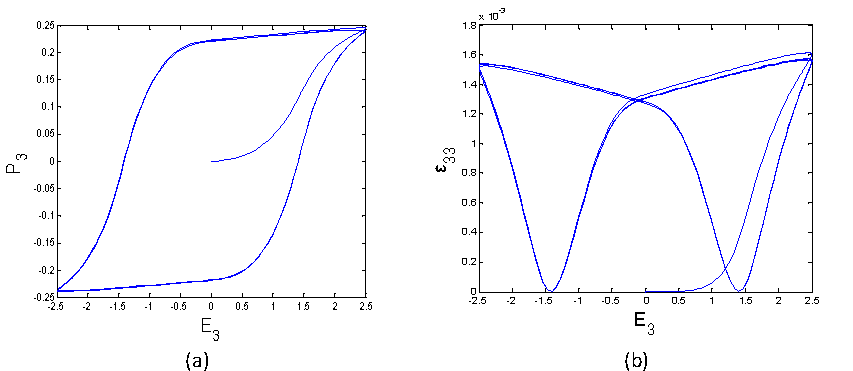
\includegraphics[width=6in]{./chap_2_pol_sw/figures/majorloop_polarization_switching.pdf}
\caption{Major hysteresis loops in a piezoelectric sample: a) polarization response and b) corresponding strain response}
\label{fig:Majorhysteresisloops}
\end{figure} 

For practical application purposes, the materials need to be polarized/poled in order to have an electro-mechanical coupling. 
This is done by applying a relatively large electric field, greater than the coercive electric field ($E_c$) of the material,
 until it reaches the saturated polarization,
  which is often done at elevated temperatures but below the Curie temperature of the material \cite{Lines1977},
   then the temperature is decreased to room temperature prior to removing the electric field which results in a remanent polarization. 
At this stage, the polarized material would have piezoelectric effects, as shown by the minor loops in figure \ref{fig:Manorhysteresisloops}. 
By applying an electric field, the polarized material would undergo mechanical deformations or experience stresses and when a mechanical load is applied the polarized material would generate electric charge or voltage difference. 
Typically, electric fields and/or mechanical stresses should be applied to the piezoelectric materials with their magnitude less than the coercive limit so that they will not cause depolarization of the materials. 
Applying large electric field or compressive stress in the poling direction to the polarized materials would cause depolarization and  consequently loss of the electro-mechanical coupling properties. 
The stress and electric field threshold that causes depolarization are called coercive stress and coercive electric field, respectively \cite{Sohrabi201344}.

\begin{figure}
\centering
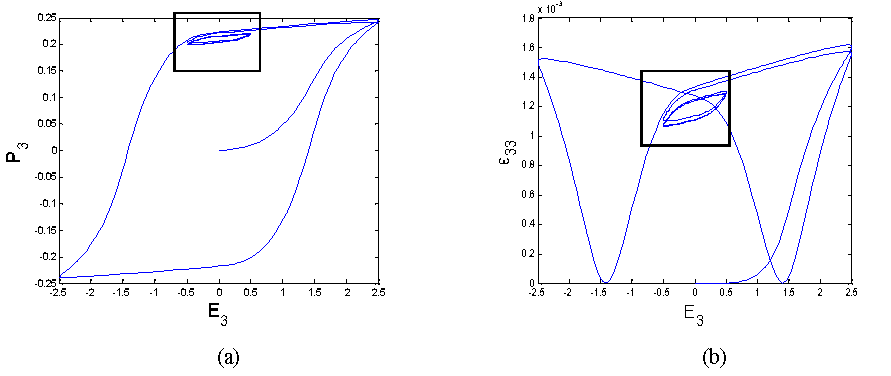
\includegraphics[width=6in]{./chap_2_pol_sw/figures/minorloop_polarization_switching.pdf}
\caption{Minor hysteresis loops in a polarized piezoelectric sample: a) polarization response and b) corresponding strain response}
\label{fig:Manorhysteresisloops}
\end{figure} 

Polarization behaviors in the materials due to application of cyclic electric fields show hysteretic responses (see figure \ref{fig:Majorhysteresisloops} and figure \ref{fig:Manorhysteresisloops}). 
These responses also depend on the frequencies of the electric field inputs, ambient temperatures, and existence of mechanical loading. 

\section{Phenomenological Model}
A time-dependent hysteretic polarization model is formulated to describe the macroscopic polarization response of ferroelectric materials
 due to various histories of external electric field inputs. 
The model is then modified to include the effect of the mechanical stress on the
 polarization response of the ferroelectric materials \cite{Muliana2011,Sohrabi201344}.
Consider an electric field input in the $x_3$ direction $E_3(s),s>0$,  and $E_3(s)=0,\forall s<0$  , where $s$ is the time history.  
The corresponding polarization response at current time $t$ is:

\begin{equation}
P_3^t\equiv P_3[E_3(t-s),t]=R[E_3(t-s),t]+Q[E_3(t-s),t]
\label{EQN:polarization_decomposition}
\end{equation}
where $R[E_3(t-s),t]$ is the time-dependent reversible polarization response at current time $t\geq 0$ with $R[0,t]=0$ and $Q[E_3(t-s),t]$ is the residual (irreversible) polarization. The reversible polarization response is expressed as:

\begin{equation}
\label{EQN:RevPol}
R^t\equiv R[E_3(t-s),t]= R[E_3^0,t]+\int_{0^+}^t\frac{\partial R}{\partial E_3} [E_3^t,t-s] \frac{dE_3^s}{ds}ds , t \geq 0
\end{equation}

\begin{equation}
R[E_3^0,t]=R_0(E_3^0)+R_1(E_3^0)\big(1-exp\bigg[-\frac{t}{\tau_1}\bigg] \big)
\label{EQN:StaticRevPol}
\end{equation}

One may consider $R[E_3^0,t]$ as the polarization at current time $t$ due to a constant electric field applied at $s=0$. 
The superscript $s$ and $t$ denote the representative of the previous time history and current time, respectively.
 Both $R_0(E_3^s)$ and $R_1(E_3^s)$ are functions of $E_3^s$. The characteristic time $\tau_1$ measures the speed that the polarization changes with time.
 For a linear electric behavior $R_0(E_3^s)$ and $R_1(E_3^s)$ are considered as follows:

\begin{equation}
\begin{aligned}
&R_0(E_3^s)=\kappa_0 E_3^s \\
&R_1(E_3^s)=\kappa_1 E_3^s
\end{aligned}
\label{EQN:R0R1Defini}
\end{equation}
where $\kappa_0$ is the dielectric constant of a macroscopically non-polarized material
 (corresponding to the second order permeability tensor in a multi-axial case) and $\kappa_1$ is the time dependent dielectric constant;
 when $\kappa_1=0$ ,
 a time-independent polarization behavior is considered. 
The state of polarization is defined through the following polarization function:
 
\begin{equation}
\label{EQN:SurfacePol}
f(P_3^t,P_c)=\left< {P_3^t}^2-P_c^2 \right> 
\end{equation}
where $P_c$ is the current polarization state,
 analogous to yield stress in an over stress plasticity theory,
  and $<>$ are the Macaulay brackets.
It is assumed that the irreversible polarization is formed when $f(P_3^t,P_c)=0$ and $E_3^t P_3^t>0$. 
The irreversible polarization is defined as:

\begin{equation}
Q^t\equiv Q[E_3^t]= \int_{0^+}^{E_3^t}\frac{d Q^s}{d E_3}{dE_3}
\label{EQN:IrrevePol}
\end{equation}

\begin{equation}
\frac{d Q^t}{d E_3}=
\begin{cases}

\lambda|\frac{E_3^t}{E_c}|^n & \text{if } |E_3^t|\leq E_c, f=0 \\
\mu \times exp[-\omega(\frac{|E_3^t|}{E_c}-1)] & \text{if }|E_3^t|> E_c, f=0 \\ 0
& \text{if } f \leq 0 

\end{cases}
\label{EQN:TimeDepIrrevePol}  
\end{equation}
where $E_c$ is the coercive electric field and $\lambda,\mu,\omega,n$ are material parameters that are calibrated from experiments. 
In a non-polarized sample, the current polarization state $P_c=0$,
 and once the ferroelectric sample is completely polarized, 
the current polarization state is equal to the saturated polarization ($P_c=P_s$ or $P_c=-P_s$) see refrence \cite{Muliana2011}.
Ferroelectric materials exhibit macroscopic electro-mechanical coupling response when they are macroscopically polarized. 
This is shown by an elongation in the material along the electric field line and a contraction in the transverse directions when the electric field is applied in the poling direction. 
When the electric field is applied opposite to the poling direction,
 the material experiences shortening along the electric field line and expansion in the transverse directions and when the electric field is applied perpendicular to the poling directions,
  the transverse shear deformations are shown. 
The macroscopic strains due to the polarization are measured through the piezoelectric constant $\mathbf{g(P^t_3)}$ whose magnitude depends on the polarization state.
The polarized ferroelectric material could experience depolarization $P^t_3=0$ when a sufficient electric field is applied in the opposite direction to its poling axis.
When the depolarization occurs, the materials loose their electro-mechanical coupling effect, which is represented by $\mathbf{g(0)=0}$. 
Polarizing the ferroelectric material by applying an electric field,
 while at the same time the ferroelectric material is under a compressive stress along the electric field line, 
 results in reductions of the saturated and remanent polarizations and the coercive electric field. 
A nonlinear electro-mechanical coupling constitutive model for ferroelectric ceramics undergoing small deformations that
 incorporates changes in the polarization due to an electric field while
 undergoing mechanical stresses is:
 
\begin{equation}
\begin{aligned}
&{ {\varepsilon }}_{{ {ij}}}^{ {t}}{ { = }}{{ {S}}_{{ {ijkl}}}}{ {\sigma }}_{{ {kl}}}^{ {t}}{ { + 4g}}_{{ {nij}}}^{ {t}}{{ {\kappa }}_{{ {nm}}}}{ {g}}_{{ {mkl}}}^{ {t}}{ {\sigma }}_{{ {kl}}}^{ {t}}{ { + 2 g}}_{{ {kij}}}^{ {t}}{ {P}}_{ {k}}^{ {t}} \\
&{ {D}}_{ {i}}^{ {t}}{ { = 2}}{{ {\kappa }}_{{ {im}}}}{ {g}}_{{ {mkl}}}^{ {t}}{ {\sigma }}_{{ {kl}}}^{ {t}}{ { + P}}_{ {i}}^{ {t}}\\
\end{aligned}
\label{EQN:3d_pol_constitutive_equation}
\end{equation}
where $S_{ijkl}$ is the scalar component of the elastic compliance tensor measured at fixed electric field,
$\sigma^t_{ij}, D^t_i, P^t_i$  are the scalar components of the mechanical stress,
 electric displacement and polarization, respectively,
 $\kappa_{ij}$  is the scalar component of the permittivity constant of a polarized specimen measured at fixed stress and constant (remanent) polarization
 $P_r$, and the small strain is defined as ${\varepsilon _{ij}} = \frac{1}{2}\left( {{u_{i,j}} + {u_{j,i}}} \right)$ , where $u_{i}$ is the scalar component of the displacement. The scalar component of the piezoelectric constant $g^t_{ijkl}$ depends on the current polarization state $P^t_3$:

\begin{equation}
g_{ijk}^t \equiv {g_{ijk}}(P_3^t) = \frac{{P_3^t}}{{{P_r}}}{e^{ - \left| {P_3^t} \right|/{C_1}}}g_{ijk}^r
\label{EQN:3d_piezo_electric_comstant_g}
\end{equation}
where $P_r$ is the remnant polarization, $C_1$ is the material parameter that needs to be calibrated from experiment (see \cite{Muliana2011}), and $g_{ijk}^r$ is the scalar component of the piezoelectric constant measured at constant polarization. 
 Thus, the constitutive model in equation (\ref{EQN:3d_pol_constitutive_equation}) is a nonlinear function of electric field and depends on time. 
 The third component of the polarization  in equation (\ref{EQN:3d_pol_constitutive_equation}) is given in equation (\ref{EQN:polarization_decomposition}),
  while the other two components are 
\begin{equation}
\begin{aligned}
& P_1^t = {\kappa _{11}}E_1^t \\
& P_2^t = {\kappa _{22}}E_2^t
\end{aligned}
\label{EQN:other_components_of_pr} 
\end{equation}  
Experimental studies show that the coercive electric field of ferroelectric materials depends on the compressive stress applied to the material along its poling direction,
 while little is known about the effect of tensile stress on the polarization response of ferroelectric ceramics. 
 This is due to the fact that ceramics is brittle and has a relatively low ultimate strength under tension. 
 It then is necessary to have the coercive electric field varies with the compressive stresses and we further assume that the coercive electric field remains unaltered with the tensile stress:

\begin{equation}
    E_c=\begin{cases}
               E_c \left( E_c^o , \sigma _{33}^{t } \right)  & \sigma _{33}^{t } < 0.0 \\
               E_c^o                                                 & \sigma _{33}^{t } \ge 0.0 
\end{cases}
\label{EQN:Effect_of_tensile_stress}
\end{equation}
 
where $E^0_c$ is the coercive electric field in absence of the mechanical stresses.
The existence of compressive stresses also influences the polarization response of ferroelectric materials. 
When a compressive stress higher than the coercive stress $\sigma_c$ is applied to the polarized ferroelectric ceramics,
 the materials undergo the polarization switching \cite{Li2004959}. 
An attempt is made to incorporate the effect of polarization switching due to a compressive stress on the overall electro-mechanical response. 
It is assumed that the compressive stress that is higher than the coercive stress limit affects the polarization state $P^t_3$ and the piezoelectric constants:
\begin{equation}
\begin{aligned}
& g_{ijk}^t \equiv {g_{ijk}}(P_3^t) = \frac{{P_3^t}}{{{P_r}}}{e^{ - \left| {P_3^t} \right|/{C_1}}}{e^{ - {C_2}\left| {\sigma _{33}^t} \right|/{\sigma _c}}}g_{ijk}^r\\
& {C_2} = 0, {\rm{ when }}, \sigma _{33}^t >  - {\sigma _c}
\end{aligned}
\label{EQN:Effect_of_tensile_stress_on_piezo_constants}
\end{equation} 
where the material parameters $\sigma_c, C_2$ have positive values and they need to be calibrated from the experimental tests.

\section{User Element Subrouine for Abaqus/UEL}
A three-dimensional (3D) continuum finite element for nonlinear time-dependent electro-mechanical response is presented here. 
The following field variables: displacements in the three directions of the Cartesian coordinate system and electric potential are sampled at each node within a finite element.
Here ${\left\{ {{{\bf{U}}^n}} \right\}^T} = \left\{ {u_1^1,u_2^1,u_3^1,...,u_1^{Nd},u_2^{Nd},u_3^{Nd}} \right\}$ and ${\left\{ {{{\bf{\Phi }}^n}} \right\}^T} = \left\{ {{\varphi ^1},{\varphi ^2},...,{\varphi ^{Nd}}} \right\}$ are the nodal displacement and electric potential vectors,
 respectively, in a single element with a number of nodes \textit{Nd}. 
 The mapping of the field variables is done through the use of shape functions $\left\{ {{N^1},{N^2},...,{N^{Nd}}} \right\}$:
\begin{equation}
\begin{aligned}
&{u_k} = \sum\limits_{i = 1}^{Nd} {{N^i}u_k^i} \begin{array}{*{20}{c}}
{}&{}&{k = 1,2,3}
\end{array}\\
&\varphi  = \sum\limits_{i = 1}^{Nd} {{N^i}\varphi _{}^i} 
\end{aligned}
\label{EQN:FEM_uel_shape_funtions}
\end{equation} 

The corresponding strains and electric fields,
 which are sampled at the material integration points within the finite element,
  are obtained as:
\begin{equation} 
\begin{aligned}
&{\varepsilon _{ij}} = \frac{1}{2}\left( {{u_{i,j}} + {u_{j,i}}} \right) = B_{ijm}^uU_m^n  & {\bf{\varepsilon }} = {{\bf{B}}^u}{{\bf{U}}^n}\\
&{E_i} =  - \frac{{\partial \varphi }}{{\partial {x_i}}} = B_{im}^\varphi \varphi _m^n  & {\bf{E}} = {{\bf{B}}^\varphi }{{\bf{\Phi }}^n}
\end{aligned}
\label{EQN:FEM_uel_shape_funtions_strain} 
\end{equation}   
where $\mathbf{B^u}$ and $\mathbf{ B^{\phi} }$ are the spatial derivative of the shape functions related to the macroscopic strain and electric field, respectively. 
The stress and electric displacement counterparts are determined using the constitutive relation discussed previously. %TK
The overall governing equations for the electro-mechanical deformation are formed at the structural level by imposing the energy balance equations. 
In this study, the nonlinear time-dependent electro-mechanical constitutive model is
 expressed in terms of the stress and electric field components as the independent field variables,
  while the displacement based finite element formulation leads to strain and electric field components as the independent variables.
Thus, the constitutive model in previous sections cannot be directly implemented in the finite element.
The nonlinear time-dependent response is solved incrementally by linearizing the response and iteratively correcting the residual (error) from the linearized solutions. 
It is necessary to define the consistent tangent stiffness, piezoelectric and dielectric constants.

\subsection{Time-Integration Algorithm at The Material Level}
The electro-mechanical constitutive model, equation (\ref{EQN:3d_pol_constitutive_equation}), depends on the polarization state $P^t_3$ ,
 which is a function of the electric field input $E^s_3$. 
 A time-integration algorithm is formulated based on a recursive method in order to approximate the current polarization state. 
 At each time \textit{t}, the polarization state is approximated as:
\begin{equation}
\begin{aligned}
&P_3^t \approx {R^t} + {Q^t};{\rm{    }}{Q^t}{\rm{ = }}{Q^{t - \Delta t}} + \Delta {Q^t}\\
&\Delta {Q^t} \equiv \frac{{d{Q^t}}}{{d{E_3}}}\Delta E_3^t;{\rm{     }}\Delta E_3^t = E_3^t - E_3^{t - \Delta t}
\label{EQN:polarization_state_approximation}
\end{aligned}
\end{equation}  
where the superscript $t-\Delta t$ denotes the previous time, $\Delta Q^t$ 
 is the incremental irreversible polarizations, and $\Delta Q^{t-\Delta t}$ is the history variable defining the irreversible polarization at the previous converged time. 
 The reversible polarization in equation (\ref{EQN:StaticRevPol}) is approximated as:

\begin{equation}
\begin{aligned}
{R^t} 
&= {R_0}(E_3^t) + {R_1}(E_3^t)\left( {1 - \exp \left[ { - \frac{t}{{{\tau _1}}}} \right]} \right) + \\
& \int\limits_{{0^ + }}^t {\left\{ {\frac{{\partial {R_0}(E_3^s)}}{{\partial {E_3}}} + \frac{{\partial {R_1}(E_3^s)}}{{\partial {E_3}}}\left( {1. - \exp \left[ { - \frac{{t - s}}{{{\tau _1}}}} \right]} \right)} \right\}\frac{{dE_3^s}}{{ds}}ds} \\
&={R_0}(E_3^t) + {R_1}(E_3^t) - {R_1}(E_3^0)\exp \left[ { - \frac{t}{{{\tau _1}}}} \right] - {q^t}
\label{EQN:reversible_polarization_state_approximation}
\end{aligned}
\end{equation}  
where the history variable related to the reversible polarization is: 

\begin{equation}  
\begin{aligned}
&{q^t} = \int\limits_{{0^ + }}^t {\frac{{\partial {R_1}(E_3^s)}}{{\partial {E_3}}}\exp \left[ { - \frac{{t - s}}{{{\tau _1}}}} \right]\frac{{dE_3^s}}{{ds}}ds} \\
&{\rm{  }} = \int\limits_{{0^ + }}^{t - \Delta t} {\frac{{\partial {R_1}(E_3^s)}}{{\partial {E_3}}}\exp \left[ { - \frac{{t - s}}{{{\tau _1}}}} \right]\frac{{dE_3^s}}{{ds}}ds}  + \\
& \int\limits_{t - \Delta t}^t {\frac{{\partial {R_1}(E_3^s)}}{{\partial {E_3}}}\exp \left[ { - \frac{{t - s}}{{{\tau _1}}}} \right]\frac{{dE_3^s}}{{ds}}ds} \\
\end{aligned} 
\label{EQN:history_variable_polarization}
\end{equation}  

\begin{equation}  
\begin{aligned} 
{q^t} & \approx \exp \left[ { - \frac{{\Delta t}}{{{\tau _1}}}} \right]{q^{t - \Delta t}} +\\
& \left[ {\frac{{\partial {R_1}(E_3^t)}}{{\partial {E_3}}}\frac{{\Delta E_3^t}}{{\Delta t}} + \exp \left[ { - \frac{{\Delta t}}{{{\tau _1}}}} \right]\frac{{\partial {R_1}(E_3^{t - \Delta t})}}{{\partial {E_3}}}\frac{{\Delta E_3^{t - \Delta t}}}{{\Delta t}}} \right]\frac{{\Delta t}}{2}
\end{aligned} 
\label{EQN:history_variable_}
\end{equation} 
At an initial time, ${q^t} = {q^0} = 0.0$ and  ${R^0} = {R_0}({E^0})$.
Once the polarization state is determined the electro-mechanical response of the ferroelectric materials at current time can be determined.
Within an incremental time $\Delta t$, the incremental nonlinear constitutive relation in equation (\ref{EQN:3d_pol_constitutive_equation}) can be expressed in a linearized form:
\begin{equation}   
\left\{ {\begin{array}{*{20}{c}}
\mathbf{\Delta {{\mathbf{\varepsilon }}^t}}\\
{\Delta {{\bf{D}}^t}}
\end{array}} \right\} = \left[ {\begin{array}{*{20}{c}}
{{\bf{\tilde S}}}&{{\bf{\tilde d}}{'^T}}\\
{{\bf{\tilde d}}}&{{\bf{\tilde \kappa }}}
\end{array}} \right]\left\{ {\begin{array}{*{20}{c}}
\mathbf{\Delta {{\bf{\sigma }}^t}}\\
{\Delta {{\bf{E}}^t}}
\end{array}} \right\} = \left[ {{{{\bf{\tilde A}}}^t}} \right]\left\{ {\begin{array}{*{20}{c}}
\mathbf{\Delta {{\mathbf{\sigma }}^t}}\\
{\Delta {{\bf{E}}^t}}
\end{array}} \right\}
\label{EQN:linearized_polarization_const_eqn}
\end{equation} 
The consistent tangent compliance , piezoelectric, and dielectric constants are defined as:
\begin{equation}  
\begin{aligned} 
& {{\tilde S}_{ijkl}} \equiv \frac{{\partial \varepsilon _{ij}^t}}{{\partial {\sigma _{kl}}}} = {S_{ijkl}} + 4g_{nij}^t{\kappa _{nm}}g_{mkl}^t  & \tilde d_{kij}^{'} \equiv \frac{{\partial \varepsilon _{ij}^t}}{{\partial {E_k}}} = \frac{{\partial g_{kij}^t}}{{\partial P_3^t}}\frac{{\partial P_3^t}}{{\partial E_m^t}}P_m^t + 2 g_{mij}^t\frac{{\partial P_m^t}}{{\partial E_k^t}}\\
& {{\tilde d}_{ikl}} \equiv \frac{{\partial D_i^t}}{{\partial {\sigma _{kl}}}} = 2{\kappa _{im}}g_{mkl}^t & {{\tilde \kappa }_{ij}} \equiv \frac{{\partial P_i^t}}{{\partial {E_j}}} \\
\end{aligned} 
\label{EQN:linearized_polarization_const_derivative}
\end{equation}  
where the partial derivative of the nonlinear piezoelectric constant and polarization in equation (\ref{EQN:linearized_polarization_const_derivative}) are expressed as:
\begin{equation}  
\begin{aligned} 
&\frac{{\partial g_{kij}^t}}{{\partial P_3^t}} = \left( {\frac{1}{{{P_r}}} - \frac{{P_3^t}}{{{C_1}{P_r}}}} \right){e^{ - \frac{{\left| {P_3^t} \right|}}{{{C_1}}}}}g_{kij}^r\\
&\frac{{\partial P_1^t}}{{\partial E_1^t}} = {\kappa _{11}} \\
& \frac{{\partial P_2^t}}{{\partial E_2^t}} = {\kappa _{22}}\\ 
& \frac{{\partial P_3^t}}{{\partial E_3^t}} = {\kappa _0} + 0.5{\kappa _1} + \frac{{\partial \left( {\frac{{d{Q^t}}}{{dE_3^t}}} \right)}}{{\partial E_3^t}}\left( {E_3^t - E_3^{t - \Delta t}} \right) + \frac{{d{Q^t}}}{{dE_3^t}}
\label{EQN:linearized_polarization_const_derivative_tangent}
\end{aligned} 
\end{equation} 
As mentioned above, the constitutive model is implemented in a displacement based finite element framework, in which the strain and electric field variables are taken as the independent variables obtained from equations (\ref{EQN:FEM_uel_shape_funtions}) and the corresponding stresses and electric displacements need to be determined. 
The incremental strain and electric field at current time are obtained from $\Delta {{\bf{\varepsilon }}^t} = {{\bf{B}}^u}{{\bf{U}}^{n,t}} - {{\bf{B}}^u}{{\bf{U}}^{n,t - \Delta t}}$ and $\Delta {{\bf{E}}^t} = {{\bf{B}}^\varphi }{{\bf{U}}^{\varphi ,t}} - {{\bf{B}}^\varphi }{{\bf{U}}^{\varphi ,t - \Delta t}}$ respectively. 
For this purpose, the linearized constitutive relation in equation (\ref{EQN:linearized_polarization_const_eqn}) is rewritten as: 

\begin{equation}  
\left\{ {\begin{array}{*{20}{c}}
{\Delta {{\mathbf{\sigma }}^t}}\\
{\Delta {{\bf{D}}^t}}
\end{array}} \right\} = \left[ {\begin{array}{*{20}{c}}
{{\bf{\tilde C}}}&{ - {\bf{\tilde e}}{'^T}}\\
{{\bf{\tilde e}}}&{{\bf{\tilde \kappa }}'}
\end{array}} \right]\left\{ {\begin{array}{*{20}{c}}
{\Delta {{\mathbf{\varepsilon }}^t}}\\
{\Delta {{\bf{E}}^t}}
\end{array}} \right\} = \left[ {{{{\bf{\tilde B}}}^t}} \right]\left\{ {\begin{array}{*{20}{c}}
{\Delta {{\mathbf{\varepsilon }}^t}}\\
{\Delta {{\bf{E}}^t}}
\end{array}} \right\}
\label{EQN:linearized_polarization_const_derivative_rewritten} 
\end{equation} 
where the consistent tangent stiffness, piezoelectric constant, and dielectric constants are:
\begin{equation}  
\begin{array}{l}
{\bf{\tilde C}} = {{{\bf{\tilde S}}}^{ - 1}}{\rm{               }}{\bf{\tilde e}}{'^{\bf{T}}} = {{{\bf{\tilde S}}}^{ - 1}}{\bf{\tilde d}}{'^T}{\rm{   }}\\
{\bf{\tilde e}} = {\bf{\tilde d}}{{{\bf{\tilde S}}}^{ - 1}}{\rm{              }}{\bf{\tilde \kappa }}' = {\bf{\tilde \kappa }} - {\bf{\tilde d}}{{{\bf{\tilde S}}}^{ - 1}}{\bf{\tilde d}}{'^T}
\end{array}
\label{EQN:tanget_piezoelectric}
\end{equation} 
Finally, the stresses and electric displacements at current time are:
\begin{equation}  
\begin{array}{l}
\mathbf{{\bf{\sigma }}^t} = {{\mathbf{\sigma }}^{t - \Delta t}} + \Delta {{\mathbf{\sigma }}^t}\\
{{\bf{D}}^t} = {{\bf{D}}^{t - \Delta t}} + \Delta {{\bf{D}}^t}
\end{array}
\label{EQN:stress_and_electric_displacement}
\end{equation} 
The polarization state $P^t_3$ is a function of the coercive electric field that depends on the current compressive stress $\sigma^t_{33}$. 
In the displacement based FE, the current value of stresses need to be determined from the strain and electric field inputs. 
In this study, during the incremental solution at the material level, the coercive electric field at current time is obtained as:



\begin{equation}
    E_c=\begin{cases}
               E_c \left( E_c^o , \sigma _{33}^{t - \Delta t} \right)  & \sigma _{33}^{t - \Delta t} < 0.0 \\
               E_c^o                                                 & \sigma _{33}^{t - \Delta t} \ge 0.0 
\end{cases}
\label{EQN:coercive_field}
\end{equation}

Thus, the calculated consistent tangent stiffness, piezoelectric constant, and dielectric constants in equation (\ref{EQN:stress_and_electric_displacement}) depend on the current electric field $E^t_3$ and stress from the previous time increment $\sigma^{t+\Delta t}_{33}$. 
Instead of performing an iteration at the material level, the correction due to a linearized stress is performed through an iteration scheme at the structural level.

\subsection{Solution at the Structural Level}
The governing equations for the electro-mechanical deformation under a quasi-static loading and small-deformation gradients are formed at the structural level by imposing the energy balance equations, which in absences of the body forces and body charges are:
\begin{equation}  
\begin{array}{l}
\int\limits_V {\sigma _{ij}^td\varepsilon _{ij}^tdV}  = \int\limits_A {t_i^tdu_i^tdA} \\
\int\limits_V {D_i^tdE_i^tdV}  = \int\limits_A {q_s^td\varphi _{}^tdA} 
\end{array}
\label{EQN:integration}
\end{equation}
wheret $t$ and $q_s$ are the surface traction and surface charge, respectively. 
Using the strain and electric field defined in equations (\ref{EQN:FEM_uel_shape_funtions}), respectively, the linearized constitutive model in equation (\ref{EQN:linearized_polarization_const_eqn}),
 and the principle of virtual work, the energy balance equations for one element are:

\begin{equation}  
\begin{array}{l}
\int\limits_V {d{{\bf{U}}^{nT}}{{\bf{B}}^{uT}}\left[ {{\bf{\tilde C}}{{\bf{B}}^u}{{\bf{U}}^n} - {\bf{\tilde e}}{'^T}{{\bf{B}}^\varphi }{{\bf{\Phi }}^n}} \right]dV}  = \int\limits_A {d{{\bf{U}}^{nT}}{{\bf{N}}^T}{\bf{t}}dA} \\
\int\limits_V {d{{\bf{\Phi }}^n}^T{{\bf{B}}^{\varphi T}}\left[ {{\bf{\tilde e}}{{\bf{B}}^u}{{\bf{U}}^n} + {\bf{\tilde \kappa }}'{{\bf{B}}^\varphi }{{\bf{\Phi }}^n}} \right]dV}  = \int\limits_A {d{{\bf{\Phi }}^n}^T{{\bf{N}}^T}q{}_sdA} 
\end{array}
\label{EQN:element_balance_equation}
\end{equation}
Equation (\ref{EQN:element_balance_equation}) can be rewritten as:
\begin{equation}  
\begin{aligned}
d{{\bf{U}}^{nT}}\int\limits_V {{{\bf{B}}^{uT}}{\bf{\tilde
C}}{{\bf{B}}^u}dV{{\bf{U}}^n} - \int\limits_V {{{\bf{B}}^{uT}}{\bf{\tilde 
e}}{'^T}{{\bf{B}}^\varphi }} dV{{\bf{\Phi }}^n}}  &= 
  d{{\bf{U}}^{nT}}\int\limits_A {{{\bf{N}}^T}{\bf{t}}dA} {\rm{   }} \to \\
{{\bf{K}}^{uu}}{{\bf{U}}^n} - {{\bf{K}}^{u\varphi }}{{\bf{\Phi }}^n} &= {{\bf{F}}^M}\\
d{{\bf{\Phi }}^n}^T\int\limits_V {{{\bf{B}}^{\varphi T}}{\bf{\tilde
e}}{{\bf{B}}^u}dV{{\bf{U}}^n} + \int\limits_V {{{\bf{B}}^{\varphi T}}{\bf{\tilde \kappa }}'{{\bf{B}}^\varphi }} dV{{\bf{\Phi }}^n}} & = d{{\bf{\Phi }}^n}^T\int\limits_A {{{\bf{N}}^T}q{}_sdA} {\rm{   }} \to \\
{{\bf{K}}^{\varphi u}}{{\bf{U}}^n} + {{\bf{K}}^{\varphi \varphi }}{{\bf{\Phi }}^n} &= {{\bf{F}}^E}
\end{aligned}
\label{EQN:element_balance_equation_rewritten}  
\end{equation} 

In order to obtain solutions for the displacements and electric potential at the element level the Gaussian quadrature method is used for the spatial integration. 
At each time increment the linearized relations in equations (\ref{EQN:linearized_polarization_const_derivative})-(\ref{EQN:stress_and_electric_displacement}) are used as a starting point for obtaining trial solutions to the nodal displacements and electric potential. 
The Newton-Raphson iterative method is then used to correct for the errors from the linearization. 
After assembly over all elements the overall equilibrium equation can be obtained with the residual vector at time \textit{t} :
\begin{equation}  
{{\bf{R}}^t} = \left\{ {\begin{array}{*{20}{c}}
{{{\bf{R}}^{u,t}}}\\
{{{\bf{R}}^{\varphi ,t}}}
\end{array}} \right\} = \left\{ {\begin{array}{*{20}{c}}
{{{\bf{F}}^{M,t}} - \left( {{{\bf{K}}^{uu,t}}{{\bf{U}}^{n,t}} - {{\bf{K}}^{u\varphi ,t}}{{\bf{\Phi }}^{n,t}}} \right)}\\
{{{\bf{F}}^{E,t}} - \left( {{{\bf{K}}^{\varphi u,t}}{{\bf{U}}^{n,t}} + {{\bf{K}}^{\varphi \varphi ,t}}{{\bf{\Phi }}^{n,t}}} \right)}
\end{array}} \right\}
\label{EQN:residual_equation}
\end{equation}
The above equation is solved when the boundary conditions are prescribed to the structures:
\begin{equation}  
\begin{aligned}
&{\bf{t}} = {\bf{\bar \sigma n}} &  \partial {{\rm{S}}_t}\\
&{q_s} = {\bf{\bar Dn}} & \partial {{\rm{S}}_q}\\
&{\bf{u}} = {\bf{\bar u}} &  \partial {{\rm{S}}_{\rm{u}}}\\
&\varphi  = \bar \varphi  &  \partial {{\rm{S}}_\varphi }
\end{aligned}
\label{EQN:boundary_equation}
\end{equation}
where $\textbf n $ is  the unit outward normal vector on the boundaries $\partial {S_t}$ and $\partial {S_q}$. 
It is also necessary for the boundaries to satisfy the following conditions:
\begin{equation}  
\begin{aligned}
& \partial {{\rm{S}}_t} \cup \partial {{\rm{S}}_{\rm{u}}} = \partial S & \partial {{\rm{S}}_t} \cap \partial {{\rm{S}}_{\rm{u}}} = 0 \\
& \partial {{\rm{S}}_q} \cup \partial {{\rm{S}}_\varphi } = \partial S & \partial {{\rm{S}}_q} \cap \partial {{\rm{S}}_\varphi } = 0
\end{aligned}
\label{EQN:residual_equation_2}
\end{equation}
It is noted that at the element level, the nodal displacements and electric potentials are taken as the independent field variables $\left\{ {{{\bf{X}}^t}} \right\} = \left\{ {\begin{array}{*{20}{c}} {{{\bf{U}}^{n,t}}}&{{{\bf{\Phi }}^{n,t}}} \end{array}} \right\}$ and in order to minimize the residual vector at each time due to the trial linearized solution, the independent field variables need to be corrected. 
Let \textit{k} be an iterative counter, the corrected field variables at time \textit{t} is:
\begin{equation}  
\left\{ {{{\bf{X}}^{t,k + 1}}} \right\} = \left\{ {{{\bf{X}}^{t,k}}} \right\} + {\left[ {\frac{{\partial {\bf{R}}_{}^{t,k}}}{{\partial {\bf{X}}}}} \right]^{ - 1}}{\bf{R}}_{}^{t,k}
\label{EQN:newton_raphson} 
\end{equation}
and
\begin{equation}  
{{\bf{\tilde K}}^{t,k}} \equiv \left[ {\frac{{\partial {\bf{R}}_{}^{t,k}}}{{\partial {\bf{X}}}}} \right] = \left[ {\begin{array}{*{20}{c}}
{ - {\bf{K}}_{}^{uu,t,k}{\rm{       }}{\bf{K}}_{}^{u\varphi ,t,k}}\\
{ - {\bf{K}}_{}^{\varphi u,t,k}{\rm{    }} - {\bf{K}}_{}^{\varphi \varphi ,t,k}}
\end{array}} \right]
\label{EQN:newton_raphson_then}
\end{equation}
The numerical algorithm at the structural and material levels within each time increment is summarized as follows:
\begin{enumerate}
  \item Input variables ${{\bf{U}}^{n,t - \Delta t}},{{\bf{\Phi }}^{n,t - \Delta t}},{{\bf{F}}^{M,t - \Delta t}},{{\bf{F}}^{E,t - \Delta t}},{{\bf{\tilde K}}^{t - \Delta t}},{Q^{t - \Delta t}},{q^{t - \Delta t}},{P_c}$
  \item Determine trial nodal variables at time t :${{\bf{U}}^{n,t,k}},{{\bf{\Phi }}^{n,t,k}};\begin{array}{*{20}{c}} {}&{k = 0} \end{array}$
  \item Iterate for \textit{k}=0,1,2,.. (\textit{k}=iteration counter)
  \begin{enumerate}
    \item Calculate ${\bf{E}}_{}^{t,k},P_3^{t,k},{{\bf{g}}^{t,k}},{{\bf{\tilde B}}^{t,k}},\Delta {{\bf{\sigma }}^{t,k}},\Delta {{\bf{D}}^{t,k}},{{\bf{\sigma }}^{t,k}},{{\bf{D}}^{t,k}},{{\bf{F}}^{M,t,k}},{{\bf{F}}^{E,t,k}},{{\bf{\tilde K}}^{t,k}}$
    \item Define residual (equation \ref{EQN:residual_equation}) ${{\bf{R}}^{t,k}}$ and check for $\left\| {{\bf{R}}_{}^{t,k}} \right\| \le Tol$ ; yes then go to 4 else  
    \item Correct the nodal displacement and electric potential (equation (\ref{EQN:boundary_equation}))  and go to 3.a
  \end{enumerate}
 \item Output variables ${{\bf{U}}^{n,t}},{{\bf{\Phi }}^{n,t}},
 {{\bf{F}}^{M,t}},{{\bf{F}}^{E,t}},{{\bf{\tilde K}}^t}$ and update history variables ${Q^t},{q^t},{P_c}$
\end{enumerate}  

\section{Numerical Implementation}
This section presents analyses of the electro-mechanical response of ferroelectric materials and structural components undergoing coupled mechanical loading and electric field. 
Experimental data on the polarization switching response of PZT 51, reported by Fang and Li \cite{Li2004959}, are used to validate the constitutive model. 
Parametric studies on understanding the effects of different boundary conditions and loading rates on the electro-mechanical response of the ferroelectric materials are presented. 
Finally the FE method is used to perform time-dependent analyses of smart structural components undergoing various histories of mechanical loading and electric fields.

\subsection{Verification of the Constitutive Model} 
The electro-mechanical constitutive model in equation (\ref{EQN:3d_pol_constitutive_equation}) is validated using the experimental data of PZT51 reported by Fang and Li \cite{Li2004959}. 
Figure \ref{fig:hysteresis_polarization_butterfly_strainres_ponsespzt_51_zerostress}a shows the polarization hysteretic response ($D_3-E_3$) of PZT-51 subject to a cyclic electric field at zero stress. 
The amplitude of the electric field is 1.2 MV/m with a frequency of 1 Hz. 
\begin{figure}
\centering
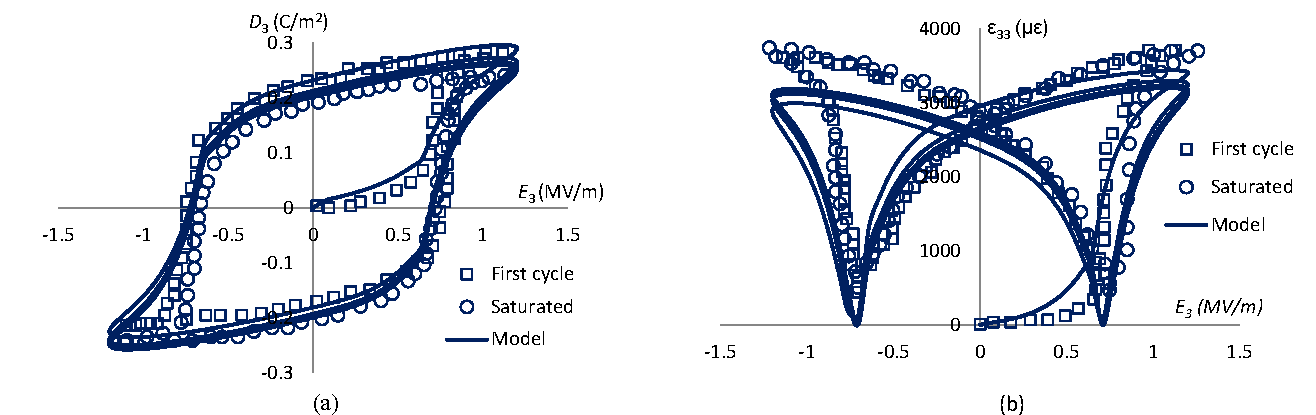
\includegraphics[width=6.0in]{./chap_2_pol_sw/figures/hysteresis_polarization_butterfly_strainres_ponsespzt_51_zero_stress.pdf}
\caption{Hysteresis polarization and butterfly strain responses for PZT51 at zero stress}
\label{fig:hysteresis_polarization_butterfly_strainres_ponsespzt_51_zerostress}
\end{figure}
The test started from an unpolarized condition and with increasing the electric field the polarization takes place. 
The loop in the first cycle is higher by about 0.03 $C/m^2$. 
After several cycles, the saturated polarization converges to a constant value, which shows a slightly smaller value than the one in the first cycle. 
The material parameters for the time-dependent polarization in equations (\ref{EQN:StaticRevPol}), (\ref{EQN:R0R1Defini}), and (\ref{EQN:3d_pol_constitutive_equation}) are calibrated from this hysteretic polarization response. 
The time-dependent polarization model is shown to be capable in capturing the hysteretic polarization response. 
The material parameters of the PZT-51 used in the simulation are reported in table \ref{table:MatPZT_51}. 
The corresponding butterfly hysteretic responses during the first and saturated cycles at zero stresses are shown in figure \ref{fig:hysteresis_polarization_butterfly_strainres_ponsespzt_51_zerostress}b. 
It is seen from figure \ref{fig:hysteresis_polarization_butterfly_strainres_ponsespzt_51_zerostress}b that at the coercive electric fields the strains from the experimental tests are nonzero, which is about 500 $\mu \varepsilon$ higher. 
This might be due to the accumulated strain from the first cycle loading. 

\begin{table}   
\caption{Material parameters for the time-dependent polarization of PZT-51}
\centering
\begin{tabular}{l c c c c c c r}
\hline 
$E_c^o$ & $\kappa_0$ & $\kappa_1$ & $\tau_1$ & $\lambda$ & $ n $ & $\mu$&  $\omega$ \\ \hline
$MV/m$ & $pF/m$ & $pF/m$ &  $sec$ & $\mu F/m$ & $\mu F/m $& $\mu F/m $\\ 
0.67\footnote{from Fang and Li \cite{raey}}&70&225&1&0.35&3&1.6&4\\ \hline
\end{tabular}
\label{table:MatPZT_51}
\end{table}

In this study, the parameter $C_1$ in equation
(\ref{EQN:Effect_of_tensile_stress_on_piezo_constants}) is calibrated from the saturated butterfly curve in figure \ref{saturated_strain_responses_pzt51_zero_stress}a after shifting the strain response obtained from the simulation 500 $\mu \varepsilon$ higher.
The piezoelectric constants measured at the remanent polarization are obtained
from Fang and \cite{Li2004959} and the permittivity constantsat the remanent polarization are taken from \cite{Muliana2011}.
It is noted that the piezoelectric constants at the remanent polarization used in equation (\ref{EQN:3d_pol_constitutive_equation}) are determined from ${{\bf{g}}^r} = {{\mathbf{\kappa }}^r}^{ - 1}{{\bf{d}}^r}$. 
\begin{figure} 
\centering
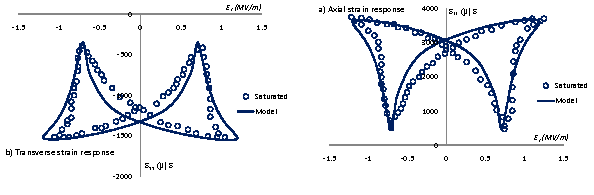
\includegraphics[width=6.0in]{./chap_2_pol_sw/figures/saturated_strain_responses_pzt51_zero_stress.pdf} 
\caption{Saturated strain responses for PZT51 at zero stress}
\label{saturated_strain_responses_pzt51_zero_stress}
\end{figure}
Tables \ref{table:MatPZT_51_Electro_mechanical_coupling} and \ref{table:MatPZT_51_Elastic_constants} report the electro-mechanical coupling parameters and elastic constants, respectively, for PZT-51. 
The corresponding transverse butterfly strain response is shown in figure \ref{saturated_strain_responses_pzt51_zero_stress}b. 
The nonlinear electro-mechanical coupling model is capable of simulating the hysteretic polarization switching electro-mechanical response.

\begin{table}
\caption{Electro-mechanical coupling parameters for PZT-51}
\centering
\begin{tabular}{l c c c c r}
\hline 
$d^r_{333}$ & $d^r_{311}$& $\kappa^r_{11}$&$\kappa^r_{33}$ & $P_r$& $C_1$ \\  \hline
$(\times 10^{-12} m/V)$ & & $(\times 10^{-9} F/m)$ &  & $C/m^2$& $C/m^2$ \\ 
$1520$ \footnote{ from Fang and Li \cite{raey}} & 570 & 38 & 42 & 0.194 & 0.19 \\  \hline
\end{tabular}
\label{table:MatPZT_51_Electro_mechanical_coupling}
\end{table}

Next, the hysteretic responses due to a cyclic electric field at various constant compressive stresses are simulated. 
Figures \ref{hysteresis_polarization_responses_under_constant_compressive_stresses} and \ref{butterfly_strain_responses_under_constant_compressive_stresses} illustrate the polarization and butterfly strain responses under a cyclic electric field with amplitude of 1.2 MV/m and frequency of 1 Hz and various compressive stresses: 5-30 MPa. 
\begin{figure} 
\centering 
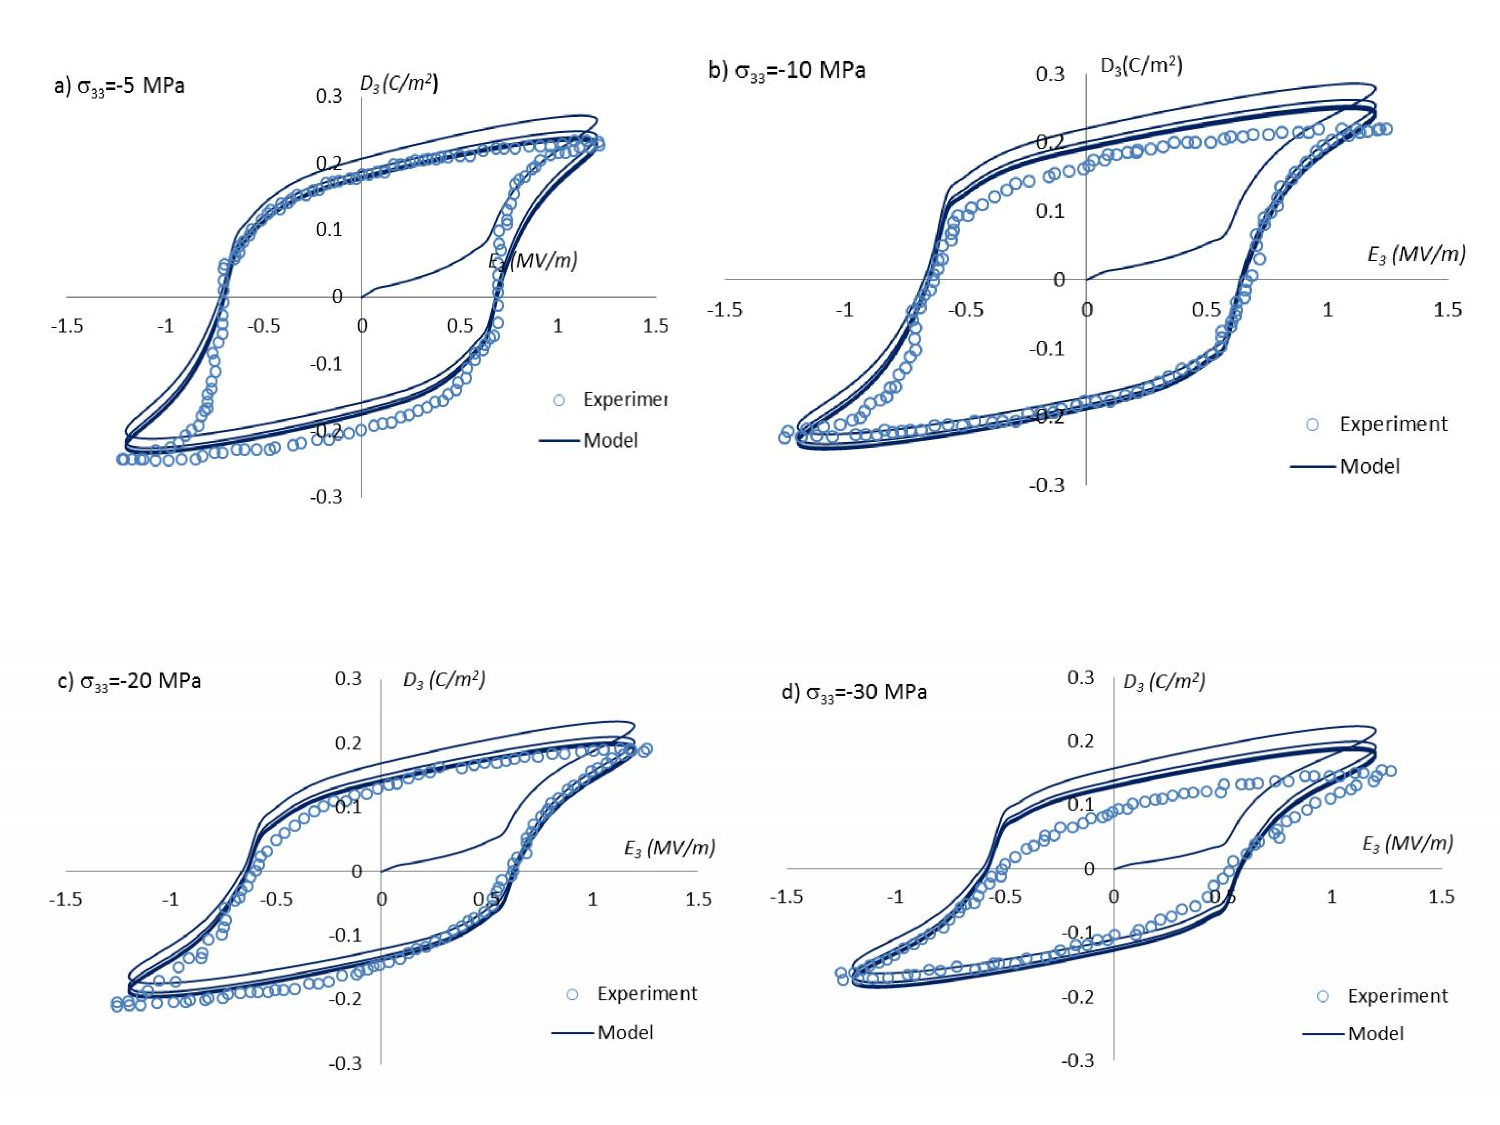
\includegraphics[width=6.0in]{./chap_2_pol_sw/figures/hysteresis_polarization_responses_under_constant_compressive_stresses.pdf} 
\caption{Hysteresis polarization responses under constant compressive stresses}
\label{hysteresis_polarization_responses_under_constant_compressive_stresses}
\end{figure}
\\

\begin{figure}
\centering 
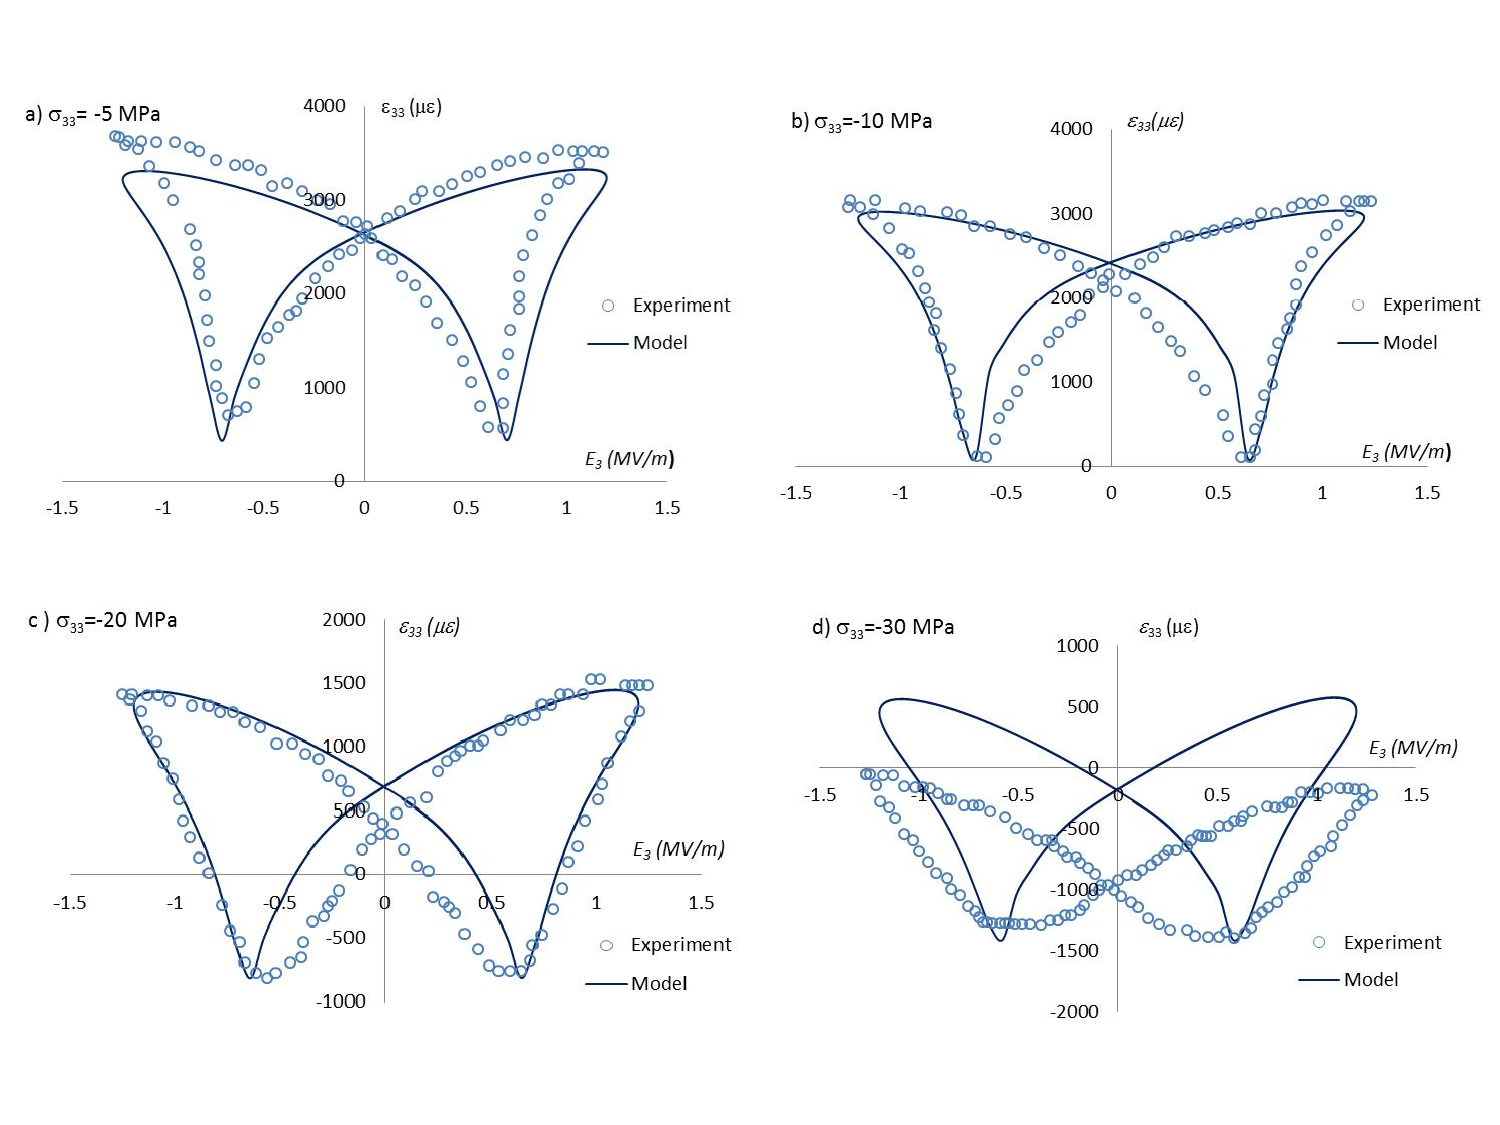
\includegraphics[width=6.0in]{./chap_2_pol_sw/figures/butterfly_strain_responses_under_constant_compressive_stresses.pdf} 
\caption{Butterfly strain responses under constant compressive stresses}
\label{butterfly_strain_responses_under_constant_compressive_stresses}
\end{figure}
From the experimental evidences the coercive electric fields vary with the compressive stresses, which can be described by the following function:
\begin{equation}  
{E_c} = E_c^o - 0.0041\left| {\sigma _{33}^t} \right|
\label{EQN:effect_of_stress_on_coercive_field}
\end{equation}

\begin{table}
\caption{Elastic constants for PZT-51 \cite{Muliana2011}}
\centering
\begin{tabular}{l c c c c r} 
\hline 
$E_{11}=E_{22}$ & $E_{33}$& $G_{12}(GPa)$&$G_{13}=G_{23}$ & $\nu{12}$& $\nu_{13}=\nu_{23} $ \\  \hline
34.48 & 33 & 13.19 &12.37 & 0.307 & 0.334 \\  \hline
\end{tabular}
\label{table:MatPZT_51_Elastic_constants} 
\end{table}

The material parameters reported in tables \ref{table:MatPZT_51} and \ref{table:MatPZT_51_Electro_mechanical_coupling} are used in the simulation. 
Good model predictions are shown for the response up to 20 MPa compressive stresses and at the compressive stress 30 MPa,
 the model over-predicts the polarization and strain responses. 
 The effect of compressive stresses in reducing the overall axial strain and
 electric displacement is due to the electro-mechanical coupling $4g_{n33}^t{\kappa _{nm}}g_{m33}^t\sigma _{33}^t$ and $2{\kappa _{3m}}g_{m33}^t\sigma _{33}^t$ , respectively, with indices \textbf{m} and \textbf{n} vary from 1 to 3. Fang and Li \cite{Li2004959} discussed that when the ferroelectric materials are subjected to compressive stresses higher than the coercive stress $\sigma _c$ of the materials, polarization switching occurs, which can alter the material properties.
 Figures \ref{hysteresis_polarization_responses_under_constant_compressive_stresses}d and \ref{butterfly_strain_responses_under_constant_compressive_stresses}d indicate that under a compressive stress of 30 MPa the polarization switching has occurred in PZT-51 which is shown by a significantly low strain response.
In order to incorporate the effect of polarization switching due to high compressive stresses, the piezoelectric constants in Eq. (\ref{EQN:Effect_of_tensile_stress_on_piezo_constants}) is used. 
\begin{table}
\caption{Material parameters above the coercive stress limit}
\centering
\begin{tabular}{c c c c c c}
\hline
$\sigma_c (MPa)$ & $C_2$ & $\lambda (\times 10 ^6 F/m)$ & $n$ & $ \mu (\times 10^{-6} F/m) $ & $\omega$ \\ \hline
$25$ & $0.3$ & $0.4$ & $3.0$ & $1.1$ & $4$ \\ \hline
\end{tabular} 
\label{table4:Material_parameters_above_the_coercive_stress_limit}
\end{table}
The hysteretic responses under compressive stresses 30-80 MPa are shown in (figures \ref{Fig_6_hysteresis_polarization_responses_under_constant_compressive_stresses_above_the_coercive_stress} and \ref{fig_7_butterfly_strain_responses_under_constant_compressive_stresses_above_the_coercive_stress}). 
Relatively good predictions of the polarization and butterfly strains are observed.
\begin{figure} 
\centering 
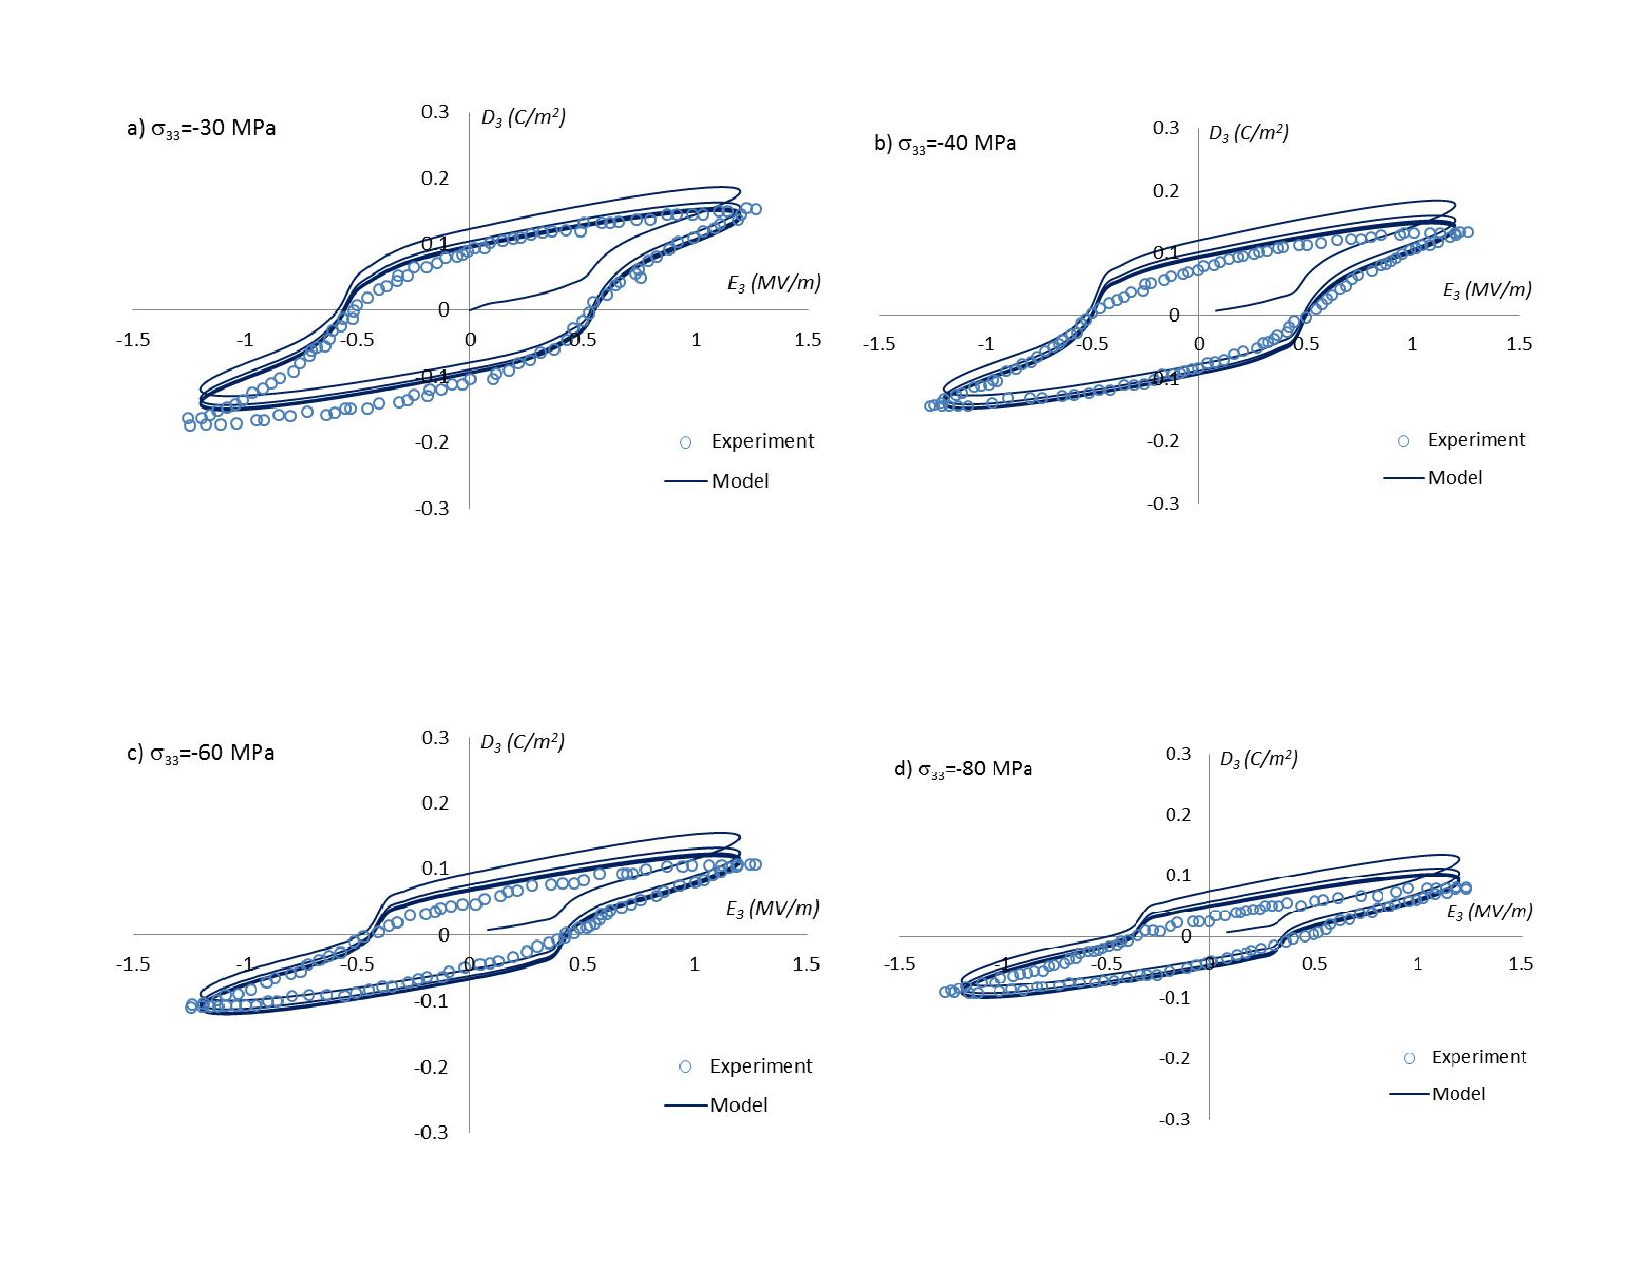
\includegraphics[width=6.0in]{./chap_2_pol_sw/figures/Fig_6_hysteresis_polarization_responses_under_constant_compressive_stresses_above_the_coercive_stress.pdf} 
\caption{Hysteresis polarization responses under constant compressive stresses above the coercive stress}
\label{Fig_6_hysteresis_polarization_responses_under_constant_compressive_stresses_above_the_coercive_stress}
\end{figure} 

\begin{figure} 
\centering 
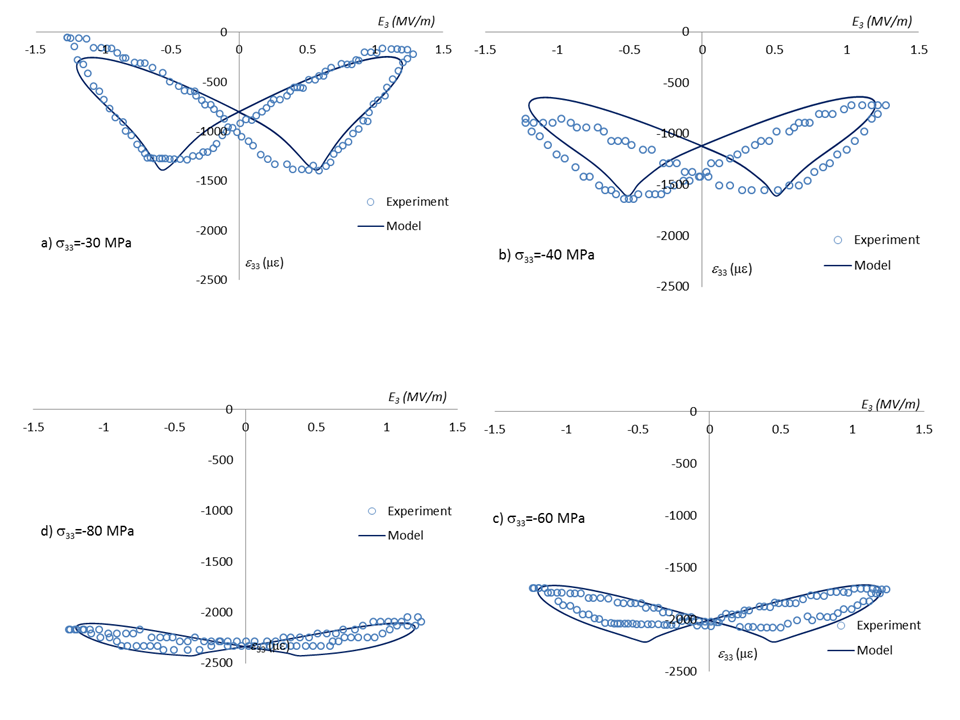
\includegraphics[width=6.0in]{./chap_2_pol_sw/figures/fig_7_butterfly_strain_responses_under_constant_compressive_stresses_above_the_coercive_stress.png} 
\caption{Butterfly strain responses under constant compressive stresses above the coercive stress}
\label{fig_7_butterfly_strain_responses_under_constant_compressive_stresses_above_the_coercive_stress}
\end{figure}
This study used the hysteretic responses under a compressive stress 40 MPa (figures \ref{Fig_6_hysteresis_polarization_responses_under_constant_compressive_stresses_above_the_coercive_stress}b and \ref{fig_7_butterfly_strain_responses_under_constant_compressive_stresses_above_the_coercive_stress}b) to calibrate the material parameters when the polarization switching occurs due to high compressive stresses.  
The coercive stress is taken as 25 MPa. 
In this study an attempt is made to recalibrate the parameters corresponding to the irreversible polarization. 
Table \ref{table4:Material_parameters_above_the_coercive_stress_limit} presents the calibrated material parameters above the coercive stress limit. 
\newpage

\subsection{Structural Analyses}
The PZT-51 is now used to induce deformations in a fiber reinforced laminated composite plate. 
Consider a composite plate (host structure) of 100x50x1 $mm^3$, shown in figure \ref{fig:ActiveComposBeam}, with four PZT patches. 
Each PZT patch has a dimension of 10x10x1 $mm^3$. 
The properties of the PZT are given in tables \ref{table:MatPZT_51}-\ref{table4:Material_parameters_above_the_coercive_stress_limit}, while the composite plate is made of a glass fiber composite. 

The composite plate is assumed linear elastic with the following elastic material properties: E=36000MPa, $\nu$=0.25 in the longitudinal fiber axis. 
The plate is clamped along one of its 50 mm side surface and the PZT patches are bonded perfectly to the host structure. 
The potential on the surfaces of the PZT patches that are in contact to the host structure is grounded to zero. 
The PZT patches are uniformly subjected to the potential gradient through their thickness ${E_3}(t) = 1.2\sin (2\pi ft){\rm{ MV/m}}$ so that they experience expansion in their planar direction, thus inducing bending to the composite plate. 
Figure \ref{fig:tipdeflectioncompositeactivebeam} depicts the lateral displacement measured at the mid section of the free end due to the input electric field applied uniformly to the four PZT patches, which show vibration of the composite plate. 

It is seen that the highest deformation occurs at the first quarter cycle, when the electric field reaches 1.2 MV/m (point A).  
Upon removal of the electric field, the remnant deformation is shown (point B) and when the electric field reaches the coercive limit of the PZT patches no deformation is shown in the plate (point C) due to depolarization of the PZT patches. 
Continuing applying the electric field until it reaches the lowest peak -1.2 MV/m (point D) trigger bending in the composite plate. 
It is also seen that due to the time-dependent effect, the highest displacement is at the first quarter cycle and after several cycles, saturation in the butterfly displacement loop is achieved. 
The corresponding deformed shapes of the composite plate at several instant of times during the first cycle are illustrated in figure \ref{fig:Figure_13_deformed_shape_active_cantilever}. 

\begin{figure}
\centering
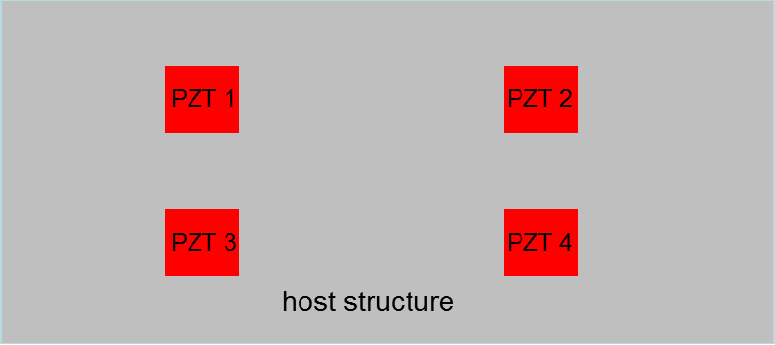
\includegraphics[width=6.0in]{./chap_2_pol_sw/figures/activecompositeplatewithpatches.pdf}
\caption{Active composite plate with PZT patches}
\label{fig:ActiveComposBeam} 
\end{figure}

\begin{figure}
\centering
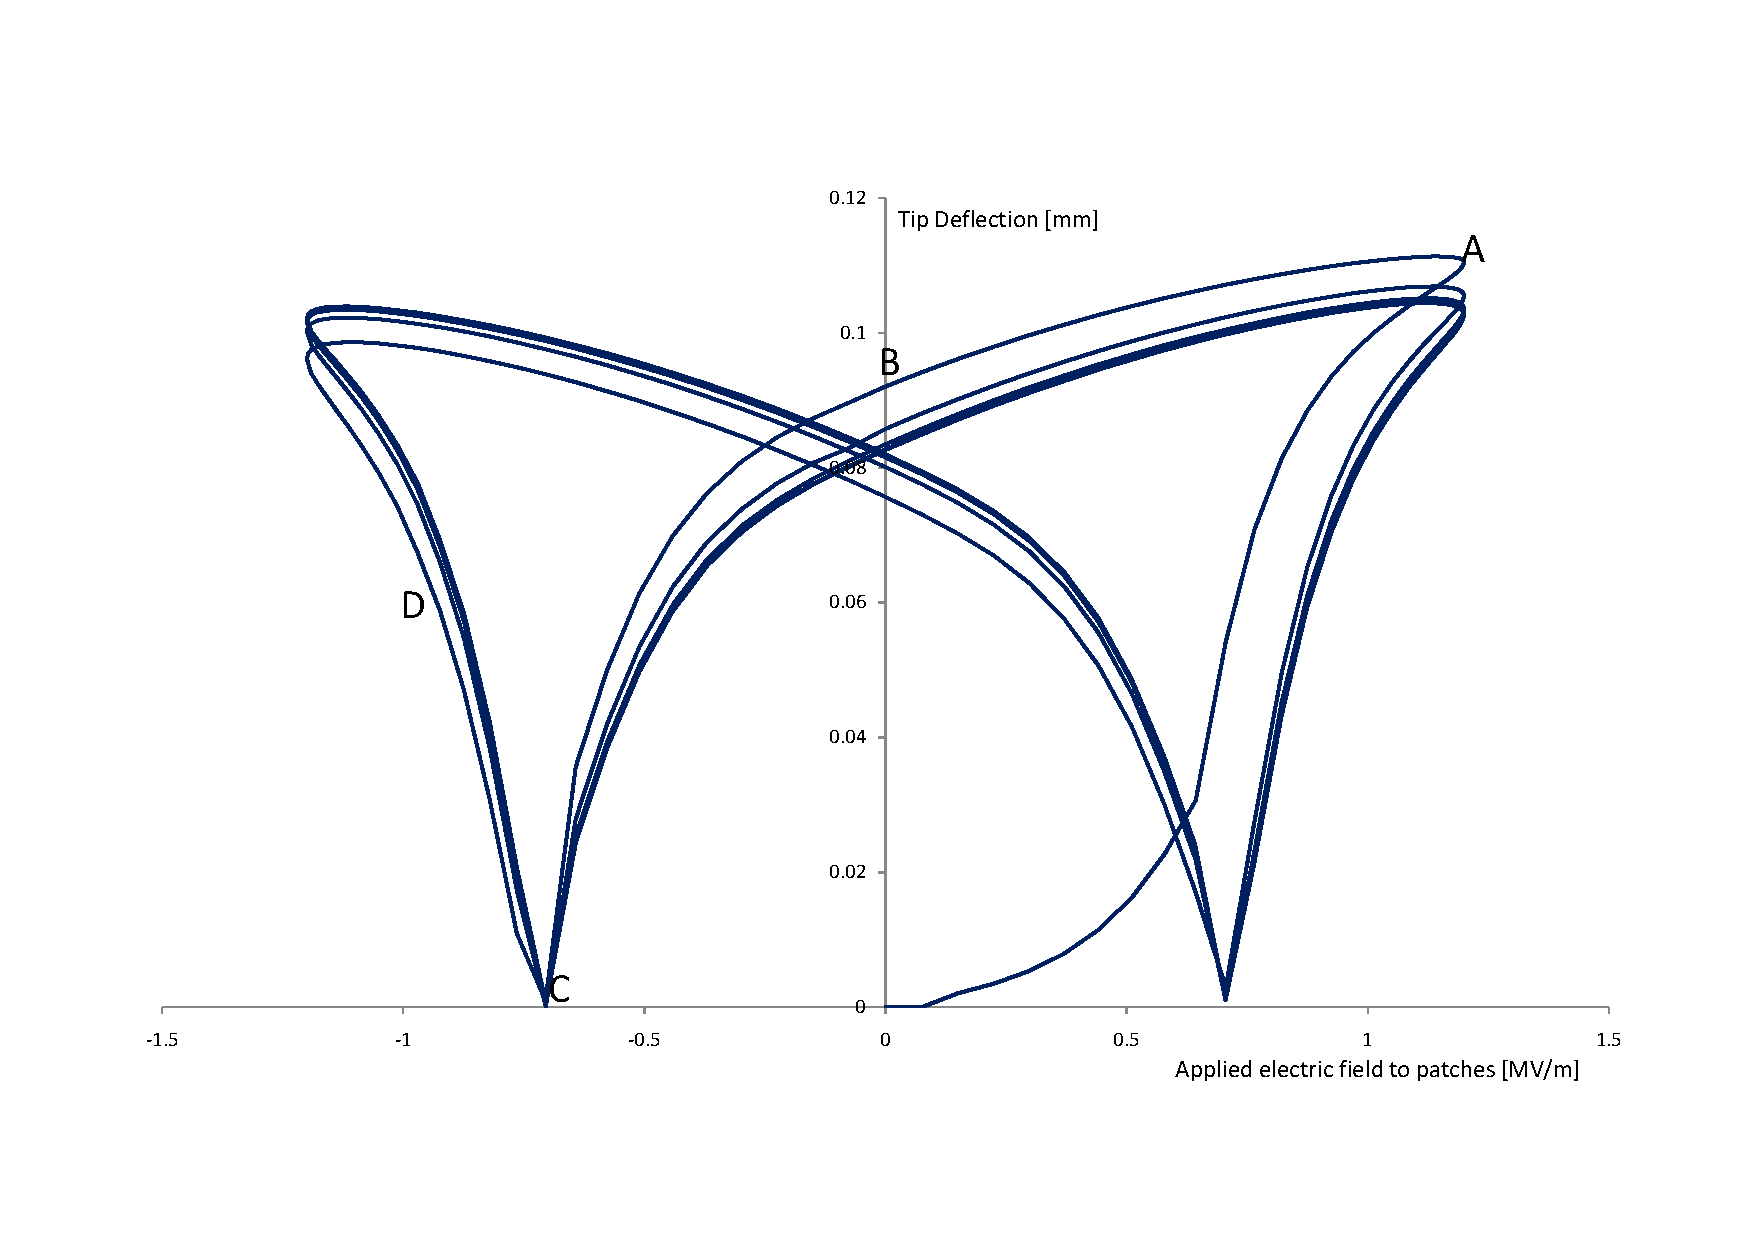
\includegraphics[width=6.0in]{./chap_2_pol_sw/figures/tipdeflectioncompositeactivebeam.pdf}
\caption{Tip deflection of the cantilever plate due to uniform cyclic electric fields applied to the piezoelectric patches}
\label{fig:tipdeflectioncompositeactivebeam}
\end{figure}
It is also possible to create different deformed shapes by considering various histories of electric field inputs. 
For example, to induce twisting of the plate different electric field inputs can be applied to the four patches. 
\begin{figure}
\centering
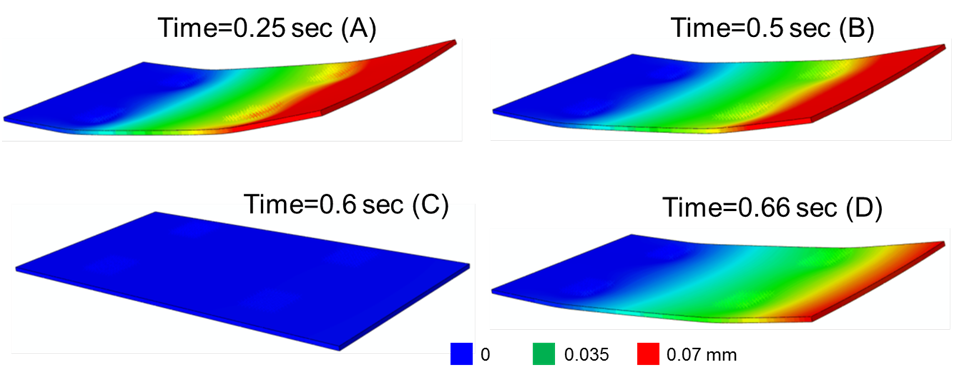
\includegraphics[width=6.0in]{./chap_2_pol_sw/figures/Figure_13_deformed_shape_active_cantilever.png}
\caption{The corresponding deformed shape of an active cantilever plate due to a uniform cyclic electric field applied to the piezoelectric patches}
\label{fig:Figure_13_deformed_shape_active_cantilever}
\end{figure}
The tip-deflection, illustrated in figure \ref{fig:Fig14_tiptwistingcompositeactivebeam}, is generated by prescribing the following electric field input to the PZT patches 3 and 4, and  to the patches 1 and 2.
\begin{figure} 
\centering
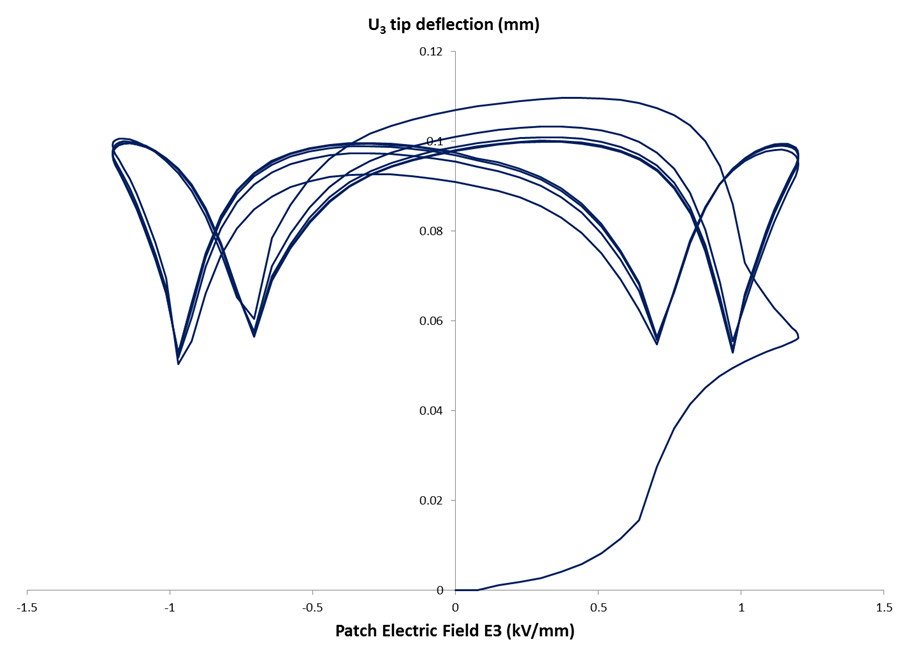
\includegraphics[width=6.0in]{./chap_2_pol_sw/figures/Fig14_tiptwistingcompositeactivebeam.png}
\caption{Tip deflection of the twisting cantilever plate due to a non-uniform cyclic electric field applied to the piezoelectric patches}
\label{fig:Fig14_tiptwistingcompositeactivebeam} 
\end{figure}

The effect of time dependent response of a viscoelastic host structures with piezoelectric patches on the overall mechanical deflection is examined. 
Figure \ref{fig:ViscoHostCompositeActiveBeam} illustrate the lateral deflection in smart beams activated by applying electric field to the patches. 
The patches are activated with the same time function with the frequency of 0.1Hz. 
The elastic host materials is made of a linear elastic material with $E=2710.03 MPa$ and $\nu = 0.35$. 
In the case of viscoelastic host structure the instantaneous elastic modulus is taken as $E=2710.03 MPa$ while the time dependent material properties are given in table \ref{table:Proney_Host}. 
It is seen that lateral deflections of the elastic and visco-elastic host structure are quite different in these two different cases. 
This could be due to delay of of the host structure for responding to internal stresses. 
This delay is caused by viscoelastic response of the host structure.

\begin{table}
\caption{Proney series for viscoelastic host structure}
\centering
\begin{tabular}{c c}
\hline
$J_n$&$\lambda_n$\\ \hline
6&2.10E-05\\ 
1&2.16E-05\\ 
0.1&1.18E-05\\ 
0.01&1.59E-05\\ 
0.001&2.16E-05\\ 
0.0001&2.01E-05\\ 
1.00E-05&6.60E-05\\ \hline
\end{tabular}
\label{table:Proney_Host}
\end{table}

A loop can be observed in the response of beam as it is shown in figure \ref{fig:ViscoHostCompositeActiveBeam}. 
As we pay close attention figure \ref{fig:ViscoHostCompositeActiveBeam} we see small loops forming the top left of the curve.
This form of response is observable in the situation where there are more than one source of hystersis response.
A looping phenomenon is evident near the extremes of the main hysteresis loop in Piezoelectric Microfiber Composite (MFC) actuators \cite{usher2013piezoelectric}.
The looping is also oserved as distorsion of hystersis loop while resistor is added to actuation circuit of PZT ($BaTiO_3$) as phase shift is introdueced to experiment \cite{jaffe2012piezoelectric}.
From observation of the experimental data and also the prediction of structural response in the simulation in figure \ref{fig:ViscoHostCompositeActiveBeam} it can be concluded that looping happens due to superposition of two different hystersis phenomena.
As an instance in the case of tip displacement of Piezoelectric Microfiber Composite (MFC) actuators \cite{usher2013piezoelectric} there are two source of hystersis.
First is the hystersis due from electromechanical coupling phenomena between electric field and mechanical responce.
Second source is the hystersis from mechanical response between stress and strain rate that happens due viscoelasticity.   

\begin{figure} 
\centering
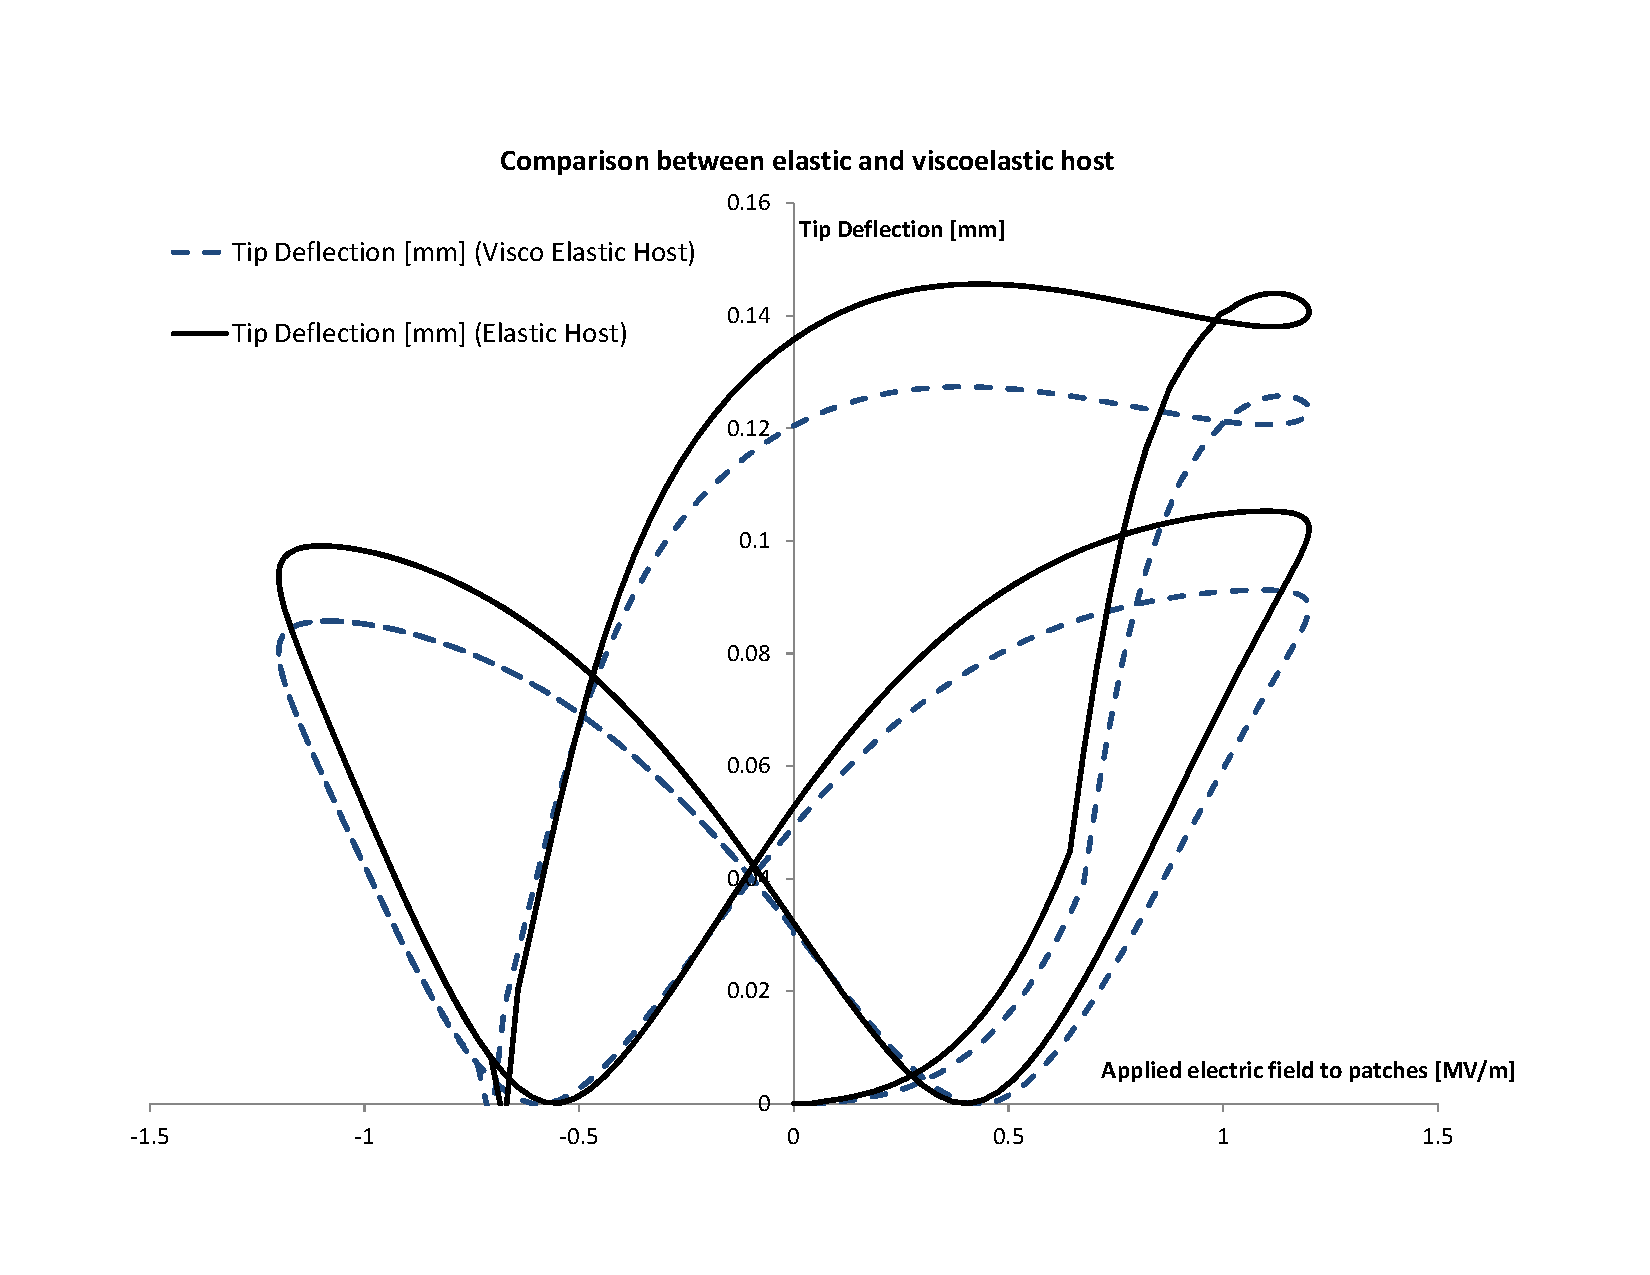
\includegraphics[width=6.0in]{./chap_2_pol_sw/figures/ViscoHostCompositeActiveBeam.pdf}
\caption{The comparison between viscoelastic and elastic materials as host structure}
\label{fig:ViscoHostCompositeActiveBeam}
\end{figure}


% %%%%%%%%%%%%%%%%%%%%%%%%%%%%%%%%%%%%%%%%%%%%%%%%%%%
%
%  New template code for TAMU Theses and Dissertations starting Fall 2012.  
%  For more info about this template or the 
%  TAMU LaTeX User's Group, see http://www.howdy.me/.
%
%  Author: Wendy Lynn Turner 
%	 Version 1.0 
%  Last updated 8/5/2012 
%
%%%%%%%%%%%%%%%%%%%%%%%%%%%%%%%%%%%%%%%%%%%%%%%%%%%

%%%%%%%%%%%%%%%%%%%%%%%%%%%%%%%%%%%%%%%%%%%%%%%%%%%%%%%%%%%%%%%%%%%%%%%
%%%                           SECTION II 
%%%%%%%%%%%%%%%%%%%%%%%%%%%%%%%%%%%%%%%%%%%%%%%%%%%%%%%%%%%%%%%%%%%%%%%

\chapter{\uppercase{minor loop constitutive model}}  
\label{section:minor_loop_constitutive_model_for_polarized_piezo_electric}
This chapter discusses a time-dependent constitutive model for polarized piezoelectric materials with an intention to capture minor hysteretic response.
The model is suitable for piezoelectric ceramics, which experience small deformation gradient, and can sustain large electric fields. 
It is assumed that the loading is within a quasi-static condition so that we neglect the inertia effect on the electro-mechanical response and ignore the energy dissipation effect. 
The constitutive model for a polarized ferroelectric ceramics is obtained from:


\begin{equation}
\begin{aligned}
&\sigma _{ij} = \frac{\partial \Psi_e}{\partial \varepsilon_{ij}}\vert _{E_{k}}
\\
& D_k = -\frac{\partial \Psi_e}{\partial E_k}\vert _{\varepsilon_{ij}}\\
& \Psi_e= \hat{\Psi}_e(E_k,\varepsilon_{ij})
\end{aligned}
\label{EQN:Derivation_from_gibbs}
\end{equation}
where $\hat{\Psi}_e(E_k,\varepsilon_{ij})$ is the thermodynamics function expressed in terms of the electric field vector $E_k$ and strain tensor $\varepsilon_{ij}$. 
The notations $\vert _{E_{k}}$ and $\vert _{\varepsilon_{ij}}$ mean that the field variables are evaluated at constant $E_{k}$ and $\varepsilon_{ij}$, respectively.
The thermodynamics potentials are often expressed in a Taylor series expansion of the independent field variables that can include higher order terms. 
Following the constitutive model of Tiersten \cite{tiersten1993electroelastic}
for active materials undergoing large electric fields and small strains, 
the free energy $\hat{\Psi}_e(E_k,\varepsilon_{ij})$ at an isothermal condition is then expressed as:

\begin{equation}
\begin{aligned}
&\hat{\Psi}_e=
\sum_{i,j,k,l=1}^{3} \frac{1}{2}C_{ijkl}{\varepsilon _{ij}}{\varepsilon _{kl}}-
\sum_{k,i,j=1}^3 e_{kij}\varepsilon _{ij}E_k-
\sum_{k,j=1}^3 \frac{1}{2}\kappa _{kj}{E_j}{E_k}-\\
&
\sum_{i,j,k,l=1}^3 \frac{1}{2}\hat{b}_{klij}{E_k}{E_l}\varepsilon _{ij}+
\sum_{i,j,k,l=1}^3 \frac{1}{6}\chi_{kij}{E_i}{E_j}{E_k}+H.O.T
\end{aligned}
\label{EQN:Gibbs_Free_Energy}
\end{equation}
where $C_{ijkl}$ are the components of the elastic stiffness, $e_{kij}$ represents the components of electro mechanical coupling tensor and $\kappa _{kj}$ are the components of the electric permittivity tensor. The field variables are the stress $\sigma _{ij}$, strain $\varepsilon _{kl}$, electric displacement $D_k$, and electric field $E_j$.
Moreover, $\hat{b}_{klij}$ and $\chi_{kij}$ are the components of the fourth-order electro-mechanical tensor and third-order electric permeability tensor, respectively. 
Equation  (\ref{EQN:Gibbs_Free_Energy}) can be further expanded to include fourth, fifth, etc. order terms of electric field.
In such case, additional material paramaters are required.
It is also possible to consider only the odd or even terms of electric field in order to capture response of the material.
Using equations  (\ref{EQN:Gibbs_Free_Energy}) and (\ref{EQN:Derivation_from_gibbs}) the stress and electric displacement for piezoelectric materials undergoing small strain and large electric field are written as:
 
\begin{equation}
\begin{aligned}
&\sigma _{ij} = 
\sum_{k,l=1}^3 {C_{ijkl}}{\varepsilon _{kl}} - 
\sum_{k=1}^3 e_{kij}{E_k} -
\sum_{k,l=1}^3 \frac{1}{2}\hat{b}_{ijkl}{E_k}{E_l}\\
&{D_k} =  
\sum_{i,j=1}^3 {e_{kij}}{\varepsilon _{ij}} + 
\sum_{j=1}^3 {\kappa _{kj}}{E_j}+
\sum_{i,j,l=1}^3 \hat{b}_{klij}{E_l}\varepsilon _{ij}+
\frac{1}{2} 
\sum_{i,j=1}^3 \chi_{kij}{E_i}{E_j} \\
& (i,j,k=1 \dots 3)  
\end{aligned}
\label{EQN:Non_Linear_Constitutive_Relation}
\end{equation}

When the nonlinear terms are neglected, a linear electro-mechanical response of piezoelectric material \cite{Leo2007} is then obtained:

\begin{equation}
\begin{aligned}
&\sigma _{ij} = 
\sum_{k,l=1}^3 {C_{ijkl}}{\varepsilon _{kl}} - 
\sum_{k=1}^3 {e_{kij}}{E_k}\\
&{D_k} = 
\sum_{i,j=1}^3 e_{kij}\varepsilon _{ij} + 
\sum_{j=1}^3 \kappa _{kj}{E_j}\\
& (i,j,k=1 \dots 3)
\end{aligned}
\label{EQN:Standanrd_Constitutive_Relation}
\end{equation}

In the above expression, strains and electric fields are chosen as the independent field variables. 
In case of a finite element analysis, displacements $u_i$ and electric potential $\Phi$ are defined at nodes within finite elements. 
The field variables in the constitutive equations are obtained directly from the displacements $u_i$ and electric potential $\Phi$. 
The strain displacement relationship based on infinitesimal strain theory is defined as:

\begin{equation}
\varepsilon_{kl}=\frac{u_{k,l}+u_{l,k}}{2}
\label{EQN:Linear_Displacement}
\end{equation}
where subscript with comma ($_{,l}$) means derivative with respect to $x_l$ ($\frac{\partial}{\partial x_l}$). 
The electric field is defined as:

\begin{equation}
E_j=-\Phi_{,j}
\label{EQN:Linear_Electric_Field}
\end{equation}

For a linear electro mechanical response given in equation
(\ref{EQN:Standanrd_Constitutive_Relation}) the derivatives of the stress and
electric displacement with respect to the independent field variabless result in
the following material parameters:

\begin{equation}
\begin{aligned}
&\frac{\partial \sigma_{ij}}{\partial \varepsilon_{kl}}=C_{ijkl} \\
&\frac{\partial \sigma_{ij}}{\partial E_{k}}=-e_{kij} \\
&\frac{\partial D_{k}}{\partial\varepsilon_{ij}}=e_{kij} \\
&\frac{\partial D_{k}}{\partial E_{i}}=\kappa_{ki}
\end{aligned}
\label{EQN:Linear_Constants}
\end{equation}

For the nonlinear electro-mechanical model such as in equation (\ref{EQN:Non_Linear_Constitutive_Relation}),
the derivatives of the stress and electric displacament with respect to the independent field variables are:

\begin{equation}
\begin{aligned}
&\frac{\partial \sigma_{ij}}{\partial \varepsilon_{kl}}=C_{ijkl} \\
&\frac{\partial \sigma_{ij}}{\partial E_{k}}=
-e_{kij}-
\sum_{l=1}^3 \hat{b}_{klij} E_l\\
&\frac{\partial D_{k}}{\partial \varepsilon_{ij}}=
e_{kij}+
\sum_{l=1}^3 \hat{b}_{klij} E_l \\
&\frac{\partial D_{k}}{\partial E_{i}}=
\kappa_{ki}+
\sum_{m,n=1}^3 \hat{b}_{kimn}\varepsilon _{mn}+
\sum_{j=1}^3 \chi_{kij} E_j\\
\end{aligned}
\label{EQN:Non_LinearLinear_Constants}
\end{equation}

Tiersten \cite{tiersten1993electroelastic} also discussed an alternative expression of the constitutive model with nonlinear electric field and small strain when stress and 
 electric field are taken as the independent field variables

\begin{equation}
\begin{aligned}
&\varepsilon _{ij} = 
\sum_{k,l=1}^3 {S_{ijkl}}{\sigma_{kl}} + 
\sum_{k=1}^3 d_{kij}{E_k} +
\sum_{k,l=1}^3 \frac{1}{2}{f}_{ijkl}{E_k}{E_l}\\
&{D_k} =  
\sum_{i,j=1}^3 {d_{kij}}{\sigma_{ij}} + 
\sum_{j=1}^3 {\kappa^{\sigma}_{kj}}{E_j}+
\sum_{i,j,l=1}^3 {f}_{klij}{E_l} \sigma _{ij}+\frac{1}{2} 
\sum_{i,j=1}^3 \chi^{\sigma}_{kij}{E_i}{E_j} \\
& (i,j,k=1 \dots 3)  
\end{aligned}
\label{EQN:Non_Linear_Constitutive_Relation_strain_bases}
\end{equation}

The elastic compliances, $S_{ijkl}$, piezoelectric constant, $d_{kij}$, and nonlinear electroelastic constants, ${f}_{ijkl}$ are:

\begin{equation}
\begin{aligned}
& S_{ijkl} =  C^{-1}_{ijkl} \\
& d_{ijk} = \sum_{m,n=1}^3 e_{imn} S_{mnjk} \\
& f_{ijkk} =\sum_{m,n=1}^3 \hat{b}_{ijmn} S_{mnkl}
\end{aligned}
\label{EQN:Non_relation_with_constants_1}  
\end{equation}

The second- and third-order electric permeability constants are measured at zero or constant stresses:

\begin{equation}
\begin{aligned}
& {\kappa^{\sigma}_{ij}}= {\hat{\kappa}_{ij}}+\sum_{m,n=1}^3  e_{imn} d_{jmn} \\
& \chi^{\sigma}_{ijk} =    \chi_{ijk}+ \sum_{m,n=1}^3 e_{imn} f_{jkmn}
\end{aligned}
\label{EQN:Non_relation_with_constants_2} 
\end{equation}

 
In analogy to the time-dependent deformation of viscoelastic materials, the nonlinear electro-elastic model developed by Tiersten \cite{tiersten1993electroelastic} is extended to include time-dependent material parameters. 
There have been several integral models developed to describe nonlinear viscoelastic behavior:
 modified superposition principle (Findley and Lai, \cite{Findley1976}),
  multiple integral model (Green and Rivlin \cite{green1959mechanics}),
   finite strain integral models (Pipkins and Rogers \cite{pipkin1968non};
    Rajagopal and Wineman \cite{Wineman2000}),
     single integral models (Pipkins and Rogers \cite{pipkin1968non}; Schapery \cite{schapery1969characterization}),
      and quasi linear viscoelastic model (Fung \cite{fung1981biomechanics}). 
The work by Green and Rivlin \cite{green1959mechanics} provides the fundamental framework for nonlinear viscoelastic response based on continuum mechanics.
 It is assumed that small changes in the input field variables cause only small changes in the corresponding output field variables;
  this can be approximated by using continuous functions in order to express the output field variables in terms of history of inputs and time-dependent material properties. 
For a nonlinear viscoelastic material,
 Green and Rivlin \cite{green1959mechanics} formed a sum of multiple integrals of the polynomial functions to incorporate history of input variables in predicting output at current time.
 This study considers two integral approaches in modelling nonlinear time-dependent electro-nechabical response of piezo electric,
  namely multiple integral and single integral based on quasi linear viscoelastic representations.
 
\section{Multiple Time Integral Method} 
The constitutive equations (\ref{EQN:Non_Linear_Constitutive_Relation}) and
(\ref{EQN:Non_Linear_Constitutive_Relation_strain_bases}) is expressed in terms of polynomial functions of independent field variables.
In analogy to the correspondence between elastic and viscoelastic materials,
 the nonlinear electro-elastic equations of Tiersten (\cite{tiersten1993electroelastic}) is modified to include the time-dependent effect (for non-aging materials):
  
\begin{equation}
\begin{aligned}
\varepsilon _{ij} (t) &=
\int_{s=0^{-}}^{t} 
\sum_{k,l=1}^3 {S_{ijkl}}(t-s)
\frac{d{\sigma_{kl}}}{ds}ds
+
\int_{s=0^{-}}^{t} 
\sum_{k=1}^3 d_{kij}(t-s)
\frac{d{E_k}}{ds}ds  \\
&+ \int_{s_1=0^{-}}^{t}
\int_{s_2=0^{-}}^{t} 
\sum_{k,l=1}^3 
\frac{1}{2}{f}_{ijkl}(t-s_1)(t-s_2)
\frac{d{E_k}}{ds_1}
\frac{d{E_l}}{ds_2}ds_1 ds_2
\\
{D_k} &=  
\int_{s=0^{-}}^{t} \sum_{i,j=1}^3 {d_{kij}}(t-s)
\frac{d{\sigma_{kl}}}{ds}ds + 
\int_{s=0^{-}}^{t} 
\sum_{j=1}^3 {\kappa^{\sigma}_{kj}}
\frac{d{E_k}}{ds}ds + \\
&+ \int_{s_1=0^{-}}^{t}
\int_{s_2=0^{-}}^{t} 
\sum_{i,j,l=1}^3 {f}_{klij}(t-s_1)(t-s_2) \frac{d{E_l}}{ds_2}\frac{d{ \sigma _{ij} }}{ds_2}ds_1  ds_2
\\
&+ 
\int_{s_1=0^{-}}^{t}
\int_{s_2=0^{-}}^{t} 
\sum_{k,l=1}^3 
\frac{1}{2}\chi^{\sigma}_{kij}(t-s_1)(t-s_2)
\frac{d{E_i}}{ds_1}
\frac{d{E_j}}{ds_2}ds_1 ds_2 \\
& (i,j,k=1 \dots 3)  
\end{aligned}
\label{EQN:double_integral_constitutive_equation}
\end{equation} 
 
It is also possible to include higher order terms of the electric field. 
In order to graphically visualize the linear and nonlinear kernel functions of time,
 a one-dimensional multiple integral forms (up to the second order) is considered:
\begin{equation}
\begin{aligned}
R(t)&=\int_{s=0^{-}}^{t} \psi_1(t-s)\frac{dI(s)}{ds}ds \\
&   +\int_{s_1=0^{-}}^{t}\int_{s_2=0^{-}}^{t}\psi_2(t-s_1,t-s_2) \frac{dI(ds_1)}{ds_1}ds_1 \frac{dI(s_2)}{s_2}ds_2
\end{aligned}
\label{EQN:double_integral_sample}
\end{equation}
where $R(t)$ is the corresponding output at current time \textit{t}, \textit{I(s)} is the input history prescribed at $0\leq s \leq t$, $\psi_1(t)$ and $\psi_2(t,t)$ are the two kernel functions.
When the kernels are assumed to increase with time, 
Figure \ref{fig:2.1.Time_dependent_kernel_functions} illustrates the linear and second order kernel functions of time 
(see Findley et al. \cite{Findley1976} for a detailed explanation). 
It is also assumed that the material response is unaltered by an arbitrary shift of the time scale, so that
 the following functions can be used for the two kernels in equation (\ref{EQN:double_integral_sample})

\begin{equation}
\begin{aligned}
 \psi_1(t-s)=& A_0+A_1 (1-e^{(-(t-s)/\tau_1)}) \\ 
 \psi_2(t-s_1,t-s_2) = & B_0+B_1 
\left(2-e^{-(t-s_1)/\lambda_1}-e^{-(t-s_2)/\lambda_2}\right)+ \\
& B_2\left(1-e^{(-(t-s_1)/\lambda_1)})(1-e^{(-(t-s_2)/\lambda_2)}\right)  
\end{aligned}
\label{EQN:double_integral_sample_second}
\end{equation}
where $A_0, A_1, B_0, B_1, \tau_1, \lambda_1, \lambda_2$ are the material parameters that need to be determined from experiments.
A set of experiments may be performed by applying the input variables at different times, say at $t=0$ and $t=s_1$.
The main disadvantage of the multiple integral forms is in difficulties characterizing the material parameters from experiments,
 even when only up to the second order kernel function is considered. 
The characterization of material parameters becomes even more complicated for the anisotropic and nonlinear time-dependent case,
 which is the case for piezoelectric ceramics. 
 In case of the third order term is included, the following third order kernel function can be considered.
\begin{equation}
\begin{aligned}
 \psi_3(t-s_1,t-s_2,t-s_3) = & C_0+C_1 
\left(3-e^{-(t-s_1)/\eta_1}-e^{-(t-s_2)/\eta_2}-e^{-(t-s_2)/\eta_3}\right)+ \\
& C_2\left(1-e^{(-(t-s_1)/\eta_1)}\right)  
     \left(1-e^{(-(t-s_2)/\eta_2)}\right)
     \left(1-e^{(-(t-s_3)/\eta_3)}\right)
\end{aligned}
\label{EQN:double_integral_sample_third_order}
\end{equation}
It is also necessary that  $\psi_3(t,t,t-s_1)=\psi_3(t-s_1,t,t)= \psi_3(t,t-s_1,t)$.
Detailed description of this method and its implementation for numerrical method is discussed in Sohrabi and Muliana \cite{Sohrabi2011}.


\section{Time Integration Method for Multiple Integral Form}
A numerical algorithm for determining time-dependent response from the multiple integral moduli is presented here. 
Let $R \left[ I(t-s),t \right] $ be the time-dependent response at current time $t \geq 0  $ due to an input history $I^s \equiv I(s) $

A general single integral representation for the response is: 

\begin{equation}
R^t \equiv R[I^s,t]=R[I^0,t]+\int_{0^+}^{t} \frac{\partial R}{\partial I}[I^s,t-s] \frac{d I^s}{d s} ds 
; (t \geq 0)
\label{2_15_eqn_Singel_integral}
\end{equation}

where
\begin{equation}
R[I^0,t]=R_0(I^0)+R_1 R(I^0) \left(1-exp \left[-\frac{t}{\tau_1} \right] \right)
\label{2_16_eqn_Singel_integral}
\end{equation}
and
\begin{equation}
\frac{\partial R}{\partial I}[I^s,t-s]=\frac{\partial R_0(I^s)}{\partial I}+\frac{\partial R_1(I^s)}{\partial I}
\left(1-exp \left[-\frac{t-s}{\tau_1} \right] \right)
\label{2_17_eqn_Singel_integral}
\end{equation}
Here a superscript is used to denote the time-dependent variables. 
A recursive method is used for solving the above integral form. 
Substituting Eqs. (\ref{2_16_eqn_Singel_integral}) and (\ref{2_17_eqn_Singel_integral}) into equation (\ref{2_15_eqn_Singel_integral}) yields:
\begin{equation}
R^t=R_0(I^t)+R_1(I^t)-R_1(I^0) exp \left[-\frac{t}{\tau_1} \right]-q^t
\label{2_18_history_eqn_Singel_integral}
\end{equation}
where
\begin{equation}
q^t=\int_{0^+}^{t} \frac{\partial R_1 (I^s) }{\partial I} exp \left[-\frac{t-s}{\tau_1} \right] \frac{d I^s}{d s} ds
\label{2_19_history_eqn_Singel_integral}
\end{equation}
is the history variable, which can be approximated as: 
\begin{equation}
q^t \approx  exp \left[-\frac{-\Delta t}{\tau_1} \right] q^{t-\Delta t}+ 
\Big[\frac{\partial R_1 (I^t) } {\partial I} \frac{d I}{d s} \mid_t
+exp \left[ \frac{-\Delta t}{\tau_1} \right]  
\frac{\partial R_1 (I^{t-\Delta t}) } {\partial I} \frac{d I}{d s} \mid_{t-\Delta t} \Big] \frac{\Delta t}{2}
\label{2_20_EQN:single_integral_history_variables}
\end{equation}
The superscript $t-\Delta t$ denotes the previous time history. 
At initial time, $q^t=q^0=0.0$ and $R^0=R_0(I^0)$. Equations (\ref{2_18_history_eqn_Singel_integral}) and (\ref{2_19_history_eqn_Singel_integral}) give the corresponding output due to an arbitrary input $I(s)$.
For the multi-axial constitutive relation, the approximate solution in equation (\ref{2_18_history_eqn_Singel_integral}) can be applied independently to each scalar component of constirutive equation.
The numerical algorithm for the multiple integral models (one-dimensional representation) with the kernels defined in equation (\ref{EQN:double_integral_sample_second}) can be approximated by applying the recursive method as discussed above. 
The linear kernel is approximated as:

\begin{equation}
\begin{aligned}
& \int_{s=0^{-}}^{t}  \psi_1(t-s) \frac{dI(s)}{d}ds \approx \\
& \left[ A_0+A_1 \right] I_t -A_1 I(0^+) exp \left[- \frac{t}{\tau_1} \right] -q^t_1\\
& q^t_1 \approx exp \left[- \frac{\Delta t}{\tau_1} \right] q^{t-\Delta t}_1 +A_1 \frac{\Delta t}{2} 
\left[ \frac{dI}{ds} \mid_t + exp \left[ - \frac{\Delta t}{\tau_1} \right]  \frac{dI}{ds} \mid_{t-\Delta t} \right]  \\
& t \geq 0 
\end{aligned}
\label{EQN_2.23:double_integral_expand}
\end{equation}

The second order kernel in equation (\ref{EQN:double_integral_sample}) is rewritten as:

\begin{equation}
\begin{aligned}
& \int_{s_1=0^{-}}^{t}\int_{s_2=0^{-}}^{t}\psi_2(t-s_1,t-s_2) \frac{dI(s_1)}{ds_1}ds_1 \frac{dI(s_2)}{ds_2}ds_2 =\\
& [B_0+B_1(2.-e^{-t/\lambda_1} -e^{-t/\lambda_1} ) +B_2 (1-e^{-t/\lambda_2}) (1-e^{-t/\lambda_2}) ]I(0^+)I(0^+)+ \\
& \int_{s_1=0^{-}}^{t}\int_{s_2=0^{-}}^{t}  \Big( B_0+B_1  \left(2-e^{-(t-s_1)/\lambda_1}-e^{-(t-s_2)/\lambda_2}\right)+ \\
& B_2\left(1-e^{(-(t-s_1)/\lambda_1)})(1-e^{(-(t-s_2)/\lambda_2)}\right) \Big)
 \frac{dI(s_1)}{ds_1}ds_1 \frac{dI(s_2)}{ds_2}ds_2 
\end{aligned}
\label{EQN_2.23:double_integral_expand_rewrited}
\end{equation}
It can be approximated by:
\begin{equation}
\begin{aligned}
& \int_{s_1=0^{-}}^{t}\int_{s_2=0^{-}}^{t}\psi_2(t-s_1,t-s_2) \frac{dI(s_1)}{ds_1}ds_1 \frac{dI(s_2)}{ds_2}ds_2 =\\
& [B_0+B_1(2.-e^{-t/\lambda_1} -e^{-t/\lambda_1} ) +B_2 (1-e^{-t/\lambda_2}) (1-e^{-t/\lambda_2}) ]I(0^+)I(0^+)+ \\
& (B_0+2B_1)( I(t)+I(0^+) )^2-B_1(I(t)+I(0^+))(f^t_1+g^t_1) +\\
& b_2( ( I(t)+I(0^+) )^2 -f^t_2( I(t)+I(0^+) )-g^t_2( I(t)+I(0^+) )+ f^t_2 g^t_2)
\end{aligned}
\label{2_24_EQN:double_integral_expand_approximated}
\end{equation}
where the history variables $f^t_1, f^t_2, g^t_1, g^t_2$ at $t>0.0$ are given as:
\begin{equation}
\begin{aligned}
& f^t_1 \approx  exp \left[-\frac{-\Delta t}{\lambda_1} \right] f^{t-\Delta t}_1+ \frac{\Delta t}{2} \left[  \frac{dI}{s_1} \mid_t+exp \left[ \frac{-\Delta t}{\lambda_1} \right]   \frac{dI}{s_1} \mid_{t-\Delta t} \right] \\
& g^t_1 \approx  exp \left[-\frac{-\Delta t}{\lambda_1} \right] g^{t-\Delta t}_1+ \frac{\Delta t}{2} \left[  \frac{dI}{s_2} \mid_t+exp \left[ \frac{-\Delta t}{\lambda_1} \right]   \frac{dI}{s_2} \mid_{t-\Delta t} \right] \\
& f^t_2 \approx  exp \left[-\frac{-\Delta t}{\lambda_2} \right] f^{t-\Delta t}_2+ \frac{\Delta t}{2} \left[  \frac{dI}{s_1} \mid_t+exp \left[ \frac{-\Delta t}{\lambda_2} \right]   \frac{dI}{s_1} \mid_{t-\Delta t} \right] \\
& g^t_2 \approx  exp \left[-\frac{-\Delta t}{\lambda_2} \right] g^{t-\Delta t}_2+ \frac{\Delta t}{2} \left[  \frac{dI}{s_2} \mid_t+exp \left[ \frac{-\Delta t}{\lambda_2} \right]   \frac{dI}{s_2} \mid_{t-\Delta t} \right] \\
\end{aligned} 
\label{2_25_EQN:double_integral_history_variables}
\end{equation}
It is noted that at initial time $f^0_1= f^0_2= g^0_1= g^0_2=0.0$ and $R(0)=A_0I(0^+)+B_0 I(0^+)I(0^+)$. 
Thus, the corresponding response due to an arbitrary input obtained from the multiple integral model is approximated as: 

\begin{equation}
\begin{aligned}
R(t) \approx 
&\left[A_0+ A_1 \right]I(t)-A_1 exp \left[- \frac{t}{\tau_1}\right] -q_1^t \\
&\left[B_0+B_1 (2-e^{-t/\lambda_1}-e^{-t/\lambda_1}) +B_2(1-e^{-t/\lambda_2})(1-e^{-t/\lambda_2}) \right]I(0^+)I(0^+)+ \\
&(B_0+2B_1)(I(t)-I(0^+))^2-B_1(I(t)-I(0^+))(f_1^t+g_1^t)+\\
&B_2\left[ (I(t)-I(0^+))^2 -f_2^t (I(t)-I(0^+)) -g_2^t (I(t)-I(0^+)) +f_2^t g_2^t\right]
\end{aligned} 
\label{2_26_EQN:double_integral_approximate_solution}
\end{equation}

For the multi-axial constitutive relation, the approximate solution in equation (\ref{2_26_EQN:double_integral_approximate_solution}) can be applied independently to each scalar component. 

\subsection{Multiple Integral Model}
This section presents a multiple integral model to simulate hysteretic response of a piezoelectric ceramics subject to a sinusoidal electric field. 
We consider up to the third order kernel function and we examine the effect of these kernel functions on the overall nonlinear hysteretic curve. 
The following material parameters are used for the simulation:
\begin{equation}
\begin{aligned}
&A_0=200 \cdot 10^{-12} m/V; A_2=100 \cdot 10^{-12} m/V \\
&\tau_1=2 sec \\
&B_0=B_1=B_2=20 \cdot 10^{-18} m^2/V^2 \\
&C_0=C_1=C_2=50 \cdot 10^{-24} m^3/V^3 \\
&\eta_1=2sec; \eta_2=5 sec  
\end{aligned}
\label{3_5_EQN:coefficients}
\end{equation}
When only the first and third kernel functions are considered, the nonlinear hysteretic response at steady state under positive and negative electric fields is identical as shown by an anti-symmetric hysteretic curve in figure \ref{figure_3_8_the_effect_of_the_higher_order_terms_on_the_hysteretic_response}a. 
The hysteretic response under the amplitude
of electric field of 0.25 MV/m shows nearly linear response. Including the second order
kernel function allows for different response under positive and negative electric fields as
seen in figure \ref{figure_3_8_the_effect_of_the_higher_order_terms_on_the_hysteretic_response}b. At low amplitude of applied electric field, nearly linear response is shown;
however this hysteretic response does not show an anti-symmetric shape with respect to the
strain and electric field axes. The contribution of each order of the kernel function depends
on the material parameters. For example the material parameters in equation (\ref{3_5_EQN:coefficients}) yield to more
pronounced contribution of the first order kernel function; while the contributions of the
second and third order kernel functions are comparable.
Intuitively, the corresponding strain response of a piezoelectric ceramics when an electric
field is applied in the poling direction (positive electric field) need not be the same as when
an electric field is applied opposite to the poling direction (negative electric field), especially
for nonlinear response due to high electric fields. Depoling could occur in the piezoelectric
ceramics when a negative electric field with a magnitude greater than the coercive electric
field is considered. Thus, to incorporate the possibility of the depoling process, the even
order kernel functions can be incorporated in the multiple time-integral model.  In order to
numerically simulate the depolarization in the piezoelectric ceramics we apply a sinusoidal
electric field input with amplitude of 1.5 MV/m. We consider the first and second order
kernel functions and use the following material parameters so that the contributions of the
first and second order kernel functions on the strain response are comparable:
\begin{equation}
\begin{aligned}
&A_0=200 \cdot 10^{-12} m/V; A_2=100 \cdot 10^{-12} m/V \\
&\tau_1=2 sec \\
&B_0=B_1=B_2=100 \cdot 10^{-18} m^2/V^2 \\
&\eta_1=2sec; \eta_2=5 sec  
\end{aligned}
\label{3_5_EQN:coefficients_}
\end{equation}

Figure \ref{figure_3_8_the_effect_of_the_higher_order_terms_on_the_hysteretic_response} illustrates the corresponding strain response from the multiple integral model
having the first and second kernel functions. The response shows an un-symmetric
butterfly-like shape. The un-symmetric butterfly-like strain-electric field response is
expected for polarized ferroelectric materials undergoing high amplitude of sinusoidal
electric field input. The nonlinear response due to the positive electric field is caused by
different microstructural changes than the microstructural changes due to polarization
switching under a negative electric field. 



\section{Quasi Linear Viscoelastic (QLV) Model} 

In an analogy to a time-dependent deformation of visco-elastic materials \cite{Wineman2000}, 
a single integral representation for formulating time dependent electro-mechanical constitutive equations is also considered.
The time dependent electromechanical model is:  

\begin{equation}
\begin{aligned}
&\sigma_{ij}(t)=
\int_{0^-}^t 
\sum_{k,l=1}^3 \frac{\partial \sigma_{ij}}{\partial\varepsilon_{kl}}(t-s,\varepsilon_{kl}(s)) \dot{\varepsilon}_{kl}(s)ds-
\int_{0^-}^t
\sum_{k=1}^3 \frac{\partial \sigma_{ij}}{\partial E_{k}}(t-s,E_k(s)) \dot{E}_k(s)ds
\\
&D_k(t)=
\int_{0^-}^t 
\sum_{i,j=1}^3 \frac{\partial D_{k}}{\partial\varepsilon_{ij}}(t-s,\varepsilon_{ij}(s))\dot{\varepsilon}_{ij}(s)ds+
\int_{0^-}^t  
\sum_{i=1}^3 \frac{\partial D_{k}}{\partial E_{i}}(t-s,E_i(s)) \dot{E}_i(s) ds
\end{aligned}
\label{EQN:TimeIntegRepConstTensor}
\end{equation}
where the overdot indicates the time derivative, 
$t$ denotes the present time and $s$ is indicates the time history. 
It is assumed that all field variables at $t<0$ are zero, and loading starts at initial time $0$.
It is assumed that the time and field dependent parts can be separated by multiplicative decomposition\footnote{The separation of variables between the time and field dependent parts
was adopted from the quasi linear viscoelastic (QLV) model proposed by Fung
\cite{fung1981biomechanics}, which is used in many biological materials.}. 
Following the Quasi Linear Viscoelastic (QLV) model, the constitutive relation in equations (\ref{EQN:TimeIntegRepConstTensor}) can be further expressed in terms of the normalized time-dependent function \cite{tscharnuter2012nonlinear,fung1981biomechanics}, where it is written as:

\begin{equation}
\begin{aligned}
\sigma_{ij}(t)= 
&\int_{0^-}^t 
\sum_{k,l=1}^{3} K^C_{ijkl}(t-s)\frac{\partial \sigma_{ij}}{\partial\varepsilon_{kl}}(\varepsilon_{kl}(s))\dot{\varepsilon}_{kl}(s)ds +\\
&\int_{0^-}^t 
\sum_{k=1}^{3} K^e_{kij}(t-s) \frac{\partial \sigma_{ij}}{\partial E_{k}}(E_k(s))  \dot{E}_{k} (s)ds
\\
D_k(t)=
&\int_{0^-}^t 
\sum_{i,j=1}^{3} K_{kij}^e(t-s) \frac{\partial D_{k}}{\partial \varepsilon_{ij}}(\varepsilon_{ij}(s))\dot{\varepsilon}_{ij}(s)ds + \\
&\int_{0^-}^t 
\sum_{i=1}^{3} K_{ki}^{\kappa}(t-s) \frac{\partial D_{k}}{\partial E_{i}}(E_i(s))  \dot{E}_{i} (s)ds
\end{aligned}
\label{EQN:NormalizedConstitutiveRelation}
\end{equation} 
where $K^C_{ijkl}$, $K^e_{kij}$ and $K^{\kappa}_{ki}$ are the normalized time-dependent tensors corresponding to the elastic, electromechanical coupling, and permittivity tensor, respectively. 
The stresses $\sigma_{ij}$, and electric displacements  $D_k$, are evaluated at time $t$ and the input history is prescribed at $0^-<s<t$.
For the time-dependent constitutive relation, the kernel functions can be chosen to be general functions of time that are in accordance with the time-dependent behaviors,  e.g., relaxation or creep like behaviors, of the materials. 
In this study a series of discrete exponential functions, often called Prony series, is used for each time dependent kernel function.
The nonlinear time-dependent response discussed in this section can be used to model hysteresis electro-mechanical response of polarized piezoelectric ceramics under a cyclic electric field. 
The kernel functions are expressed as: 

\begin{equation}
\label{EQN:LrgKProny}
\begin{aligned}
&K_{ijkl}^C(t) =
\sum_{I=0}^{NP}{}^{I}K_{ijkl}^{C} exp(-{}^{I}\lambda_{ijkl}^{C}t) \\
&K_{ijk}^e(t) =
\sum_{I=0}^{NP} {}^{I}K_{ijk}^{e} exp(-{}^{I}\lambda_{ijk}^{e}t) \\
&K_{ki}^\kappa(t) =
\sum_{I=0}^{NP}  {}^{I}K_{ki}^{\kappa} exp(-{}^{I}\lambda_{ki}^{\kappa}t) \\
\end{aligned}
\end{equation}                   
where $ {}^{I}K_{ijkl}^{C} $, $ {}^{I}K_{ijk}^{e} $, $ {}^{I}K_{ki}^{\kappa} $ , $ {}^{I}\lambda_{ijkl} $, $ {}^{I}\lambda_{ijk}^{e} $, and $ {}^{I}\lambda_{ki}^{\kappa} $ are the material parameter related to $ I^{th} $ component of Prony series of $ K_{ijkl}^C(t) $, $ K_{ijk}^e(t) $, and  $ K_{ki}^\kappa(t) $.
Equation (\ref{EQN:LrgKProny}) defines the time dependent functions, corresponding to the electro-mechanical properties.
The chosen time-dependent functions for material properties, either creep or relaxation function, are determined based on the experimental data. 
It is also possible that some terms in the properties experience relaxation and other terms experience creep responses. 
Zhou and Kamlah \cite{zhoudetermination2005} and Anderson \cite{anderson1989piezoceramic} performed experiment on PZT ceramics.
They have shown that the electric displacement in the tested piezoelectric ceramics increases with time when a constant electric field is prescribed. 
In such cases, the time-dependent electric permittivity constants should follow creep functions. 
It has also been shown that piezoelectric ceramics experience creep deformation due to constant stress, or they undergo stress relaxation when constant strain is prescribed.

When mathematical models with rather simple forms are considered for the input history and time-dependent material properties,
it is possible to obtain exact analytical solutions for the nonlinear time dependent constitutive equation.
Laplace transform method \cite{Wineman2000} is often used to determine the corresponding time-dependent field variables for the linear response of materials. 
Piezoelectric ceramics exhibit nonlinear electro-mechanical response under a relatively large magnitude of electric field. 
In dealing with nonlinear responses, numerical methods are considered for obtaining solutions to the governing equations.
Recursive integration technique has been shown to be very effective in solving the nonlinear integral problem. 
In this study, a numerical method based on the recursive approach is adopted for solving the nonlinear time-dependent electro-mechanical coupling response.
This numerical technique will be integrated into FE analyses that is explained in following sections.


Using the time dependent constitutive equations that were presented in equation (\ref{EQN:NormalizedConstitutiveRelation}) and the time kernel function that is expressed as series of exponential functions (equation (\ref{EQN:LrgKProny})) with $ {}^{I}\lambda_{ijkl}=0$, $ {}^{I}\lambda_{ijk}^{e}=0$, and $ {}^{I}\lambda_{ki}^{\kappa}=0$, 
the expanded constitutive equations are written as:


\begin{equation}
\begin{aligned} 
\sigma_{ij}(t)=
&\sum_{k,l=1}^{3} {}^{0}K_{ijkl}^{C} 
\frac{\partial \sigma_{ij}}{\partial \varepsilon_{kl}}(\varepsilon_{kl}(t)) \varepsilon_{kl}(t)+
\sum_{k=1}^{3}
{}^{0}K_{ijk}^{e}\frac{\partial \sigma_{ij}}{\partial E_{k}}(E_{k} (t)) E_{k} (t) +\\
&\int_{0^-}^t 
\sum_{k,l=1}^{3} 
\sum_{I=1}^{NP}{}^{I}K_{ijkl}^{C} exp(-{}^{I}\lambda_{ijkl}^{C}[t-s]) 
\frac{\partial \sigma_{ij}}{\partial
\varepsilon_{kl}}(\varepsilon_{kl}(s)) \dot{\varepsilon}_{kl}(s)ds +\\
&\int_{0}^t 
\sum_{k=1}^{3}
\sum_{I=1}^{NP}
{}^{I}K_{ijk}^{e}
exp(-{}^{I}\lambda_{ijk}^{e}[t-s]) \frac{\partial \sigma_{ij}}{\partial E_{k}} (E_{k} (s)) \dot{E}_{k} (s)ds
\\
D_k(t)=
&\sum_{i,j=1}^{3}
{}^{0}K_{ijk}^{e}\frac{\partial
D_{k}}{\partial \varepsilon_{ij}} (\varepsilon_{ij}(t)) \varepsilon_{ij}(t)+
\sum_{i=1}^{3}
{}^{0}K_{ki}^{\kappa}\frac{\partial D_{k}}{\partial E_{i}}(E_{i} (t)) E_{i} (t)+\\
&\int_{0^-}^t 
\sum_{i,j=1}^{3}  
\sum_{I=1}^{NP}
{}^{I}K_{ijk}^{e} exp(-{}^{I}\lambda_{ijk}^{e}(t-s))
\frac{\partial D_{k}}{\partial \varepsilon_{ij}}(\varepsilon_{ij}(s))\dot{\varepsilon}_{ij}(s)ds+\\
&\int_{0^-}^t 
\sum_{i=1}^{3} 
\sum_{I=0}^{NP}
{}^{I}K_{ki}^{\kappa}exp(-{}^{I}\lambda_{ki}^{\kappa}[t-s]) \frac{\partial D_{k}}{\partial E_{i}} (E_{i} (s)) \dot{E}_{i} (s)ds
\end{aligned}
\label{EQN:RecursiveProny}
\end{equation}

Equations (\ref{EQN:RecursiveProny}) are rewritten with the definition of history variables as follows:

\begin{equation}
\begin{aligned}
\sigma_{ij}(t)=
&\sum_{k,l=1}^{3}  
{}^{0}K_{ijkl}^{C} 
\frac{\partial \sigma_{ij}}{\partial \varepsilon_{kl}}(\varepsilon_{kl}(t))\varepsilon_{kl}(t)+
\sum_{k,l=1}^{3} 
\sum_{I=1}^{NP}
{}^{I}q_{ijkl}^{\sigma_C}(t) + \\
&
\sum_{k=1}^{3}
{}^{0}K_{ijk}^{e}\frac{\partial \sigma_{ij}}{\partial E_{k}}(E_{k} (t)) E_{k} (t)+ 
\sum_{k=1}^{3} 
\sum_{I=1}^{NP}{}^{I}q_{ijk}^{\sigma_e}(t)\\
D_k(t)=
&\sum_{i,j=1}^{3}
{}^{0}K_{ijk}^{e}\frac{\partial D_{k}}{\partial \varepsilon_{ij}}(\varepsilon_{ij}(t)) \varepsilon_{ij}(t)+
\sum_{i,j=1}^{3}
\sum_{I=1}^{NP}{}^{I}q_{kij}^{D_e}(t) +\\
&
\sum_{i=1}^{3}
{}^{0} K_{ki}^{\kappa}\frac{\partial D_{k}}{\partial E_{i}}(E_{i} (t)) E_{i} (t)+ 
\sum_{i=1}^{3}
\sum_{I=1}^{NP}
{}^{I}q_{ki}^{D_{\kappa}}(t)
\end{aligned}
\label{EQN:History_Introduction}
\end{equation}
where the variables ${}^{I}q_{ijkl}^{\sigma_C}(t) $, ${}^{I}q_{ijk}^{\sigma_e}(t)$, ${}^{I}q_{kij}^{D_e}(t)$ and ${}^{I}q_{ki}^{D_{\kappa}}(t)$ are defined to incorporate the history in the time integral constitutive equations. 
The time integral functions are split into two parts, the first part carries the integral from the beginning to the time ($t-\Delta t$) and the second part incorporates the integral within an incremental time $\Delta t$. 
The recursive method is used for all the integrations. 
Consider a simple integral with an exponential function such as $q(t)=\int_0^t exp(-\lambda [t-s])f(s)ds$.
This integral can be approximated as $q(t)\approx exp(-\lambda\Delta t) q(t-\Delta t) +\frac{\Delta t}{2} [f(t)+exp(-\lambda \Delta t ) f(t-\Delta t)]$.
This recursive scheme is used for solving the time dependent constitutive equations. 
Using the recursive integral, the history variables are given as:   

\begin{equation}
\begin{aligned}
{}^{I}q_{ijkl}^{\sigma_C}(t)= 
&exp(-{}^{I}\lambda_{ijkl}^{C}[\Delta t]){}^{I}q_{ijkl}^{\sigma_C}(t-\Delta t)+ \\
&\int_{t-\Delta t}^{t}  
{}^{I}K_{ijkl}^{C}
exp(-{}^{I}\lambda_{ijkl}^{C}[t-s])\frac{\partial \sigma_{ij}}{\partial \varepsilon_{kl}} (\varepsilon_{kl}(s)) \dot{\varepsilon}_{kl}(s)ds \\
{}^{I}q_{ijk}^{\sigma_e}(t)=
&exp(-{}^{I}\lambda_{ijk}^{e}[\Delta t]) {}^{I}q_{ijk}^{\sigma_e}(t-\Delta t)+ \\
&\int_{t-\Delta t}^{t}  
{}^{I}K_{ijk}^{e} exp(-{}^{I}\lambda_{ijk}^{e}[t-s]) \frac{\partial \sigma_{ij}}{\partial E_{k}} (E_{k} (s)) \dot{E}_{k} (s)ds \\
{}^{I}q_{ijk}^{D_e}(t)=
&exp(-{}^{I}\lambda_{ijk}^{e}[\Delta t]){}^{I}q_{ijk}^{D_e}(t-\Delta t)+\\
&\int_{t-\Delta t}^t 
{}^{I}K_{ijk}^{e} exp(-{}^{I}\lambda_{ijk}^{e}[t-s]) \frac{\partial D_{k}}{\partial \varepsilon_{ij}}(\varepsilon_{ij}(s)) \dot{\varepsilon}_{ij}(s)ds\\
{}^{I}q_{ki}^{D_{\kappa}}(t)=
&exp(-{}^{I}\lambda_{ki}^{\kappa}[\Delta t]){}^{I}q_{ki}^{D_{\kappa}}(t-\Delta t)+\\
&\int_{t-\Delta t^-}^t  
{}^{I}K_{ki}^{\kappa}
exp(-{}^{I}\lambda_{ki}^{\kappa}[t-s]) \frac{\partial D_{k}}{\partial E_{i}} (E_{i} (s)) \dot{E}_{i} (s)ds
\end{aligned}
\label{EQN:History_Discritizing}
\end{equation}

The above equations only need to be integrated within a time increment $\Delta t$. 
An approximate form of the time derivatives of field variables is taken as: $\dot{\varepsilon}_{kl} \approx \frac{\Delta \varepsilon_{kl}}{\Delta t}$ and $\dot{E}_{k}\approx \frac{\Delta E_k}{\Delta t}$. 
Upon solving the integrals in equation (\ref{EQN:History_Discritizing}) the history variables are:

\begin{equation}
\begin{aligned}
{}^{I}q_{ijkl}^{\sigma_C}(t)=&
exp(-{}^{I}\lambda_{ijkl}^{C}[\Delta t]){}^{I}q_{ijkl}^{\sigma_C}(t-\Delta t)+ \\
& \frac{{}^{I}K_{ijkl}^{C}}{2} \Big(exp(-{}^{I}\lambda_{ijkl}^{C}[\Delta t])\frac{\partial \sigma_{ij}}{\partial \varepsilon_{kl}}(\varepsilon_{kl}(t-\Delta t)) \Delta\varepsilon_{kl}(t-\Delta t) + \\
& \frac{\partial \sigma_{ij}}{\partial \varepsilon_{kl}}(\varepsilon_{kl}(t)) \Delta \varepsilon_{kl}(t) \Big) \\
{}^{I}q_{ijk}^{\sigma_e}(t)=&
 exp(-{}^{I}\lambda_{ijk}^{e}[\Delta t]) {}^{I}q_{ijk}^{\sigma_e}(t-\Delta t)+ \\
& \frac{{}^{I}K_{ijk}^{e}}{2} \Big( exp(-{}^{I}\lambda_{ijk}^{e}[\Delta t]) \frac{\partial \sigma_{ij}}{\partial E_{k}}(E_{k} (t-\Delta t )) \Delta E_{k} (t-\Delta t ) + \\
& \frac{\partial \sigma_{ij}}{\partial E_{k}} (E_{k} (t)) \Delta E_{k} (t) \Big)\\
{}^{I}q_{ijk}^{D_e}(t)=&
exp(-{}^{I}\lambda_{ijk}^{e}[\Delta t]){}^{I}q_{k}^{D_e}(t-\Delta t)+\\
& \frac{{}^{I}K_{ijk}^{e}}{2} \Big(exp(-{}^{I}\lambda_{ijk}^{e}[\Delta t]) \frac{\partial D_{k}}{\partial \varepsilon_{ij}}( \varepsilon_{ij}(t-\Delta t)) \Delta \varepsilon_{ij}(t-\Delta t) + \\
& \frac{\partial D_{k}}{\partial \varepsilon_{ij}}(\varepsilon_{ij}(t)) \Delta \varepsilon_{ij}(t)\Big) \\
{}^{I}q_{ki}^{D_{\kappa}}(t)=&
exp(-{}^{I}\lambda_{ki}^{\kappa}[\Delta t]){}^{I}q_{k}^{D_{\kappa}}(t-\Delta t)+\\
& \frac{{}^{I} K_{ki}^{\kappa}}{2} \Big( exp(-{}^{I}\lambda_{ki}^{\kappa}[\Delta t]) \frac{\partial D_{k}}{\partial E_{i}}( E_{i} (t-\Delta t)) \Delta E_{i} (t-\Delta t) + \\ 
& \frac{\partial D_{k}}{\partial E_{i}}( E_{i} (t)) \Delta E_{i} (t)\Big)
\end{aligned}
\label{EQN:History_Discritizing_Breaking_Integral}
\end{equation}

Equations (\ref{EQN:History_Introduction}) and (\ref{EQN:History_Discritizing_Breaking_Integral}) give an approximate solutions of nonlinear-time-dependent constitutive equations. 
In the above equations the strain and electric field at each time increment are the independent variables that will be determined from structural analyses.

\section{Finite Element Implementation of QLV Model}
\label{Chapter:Finite_element}
This section briefly presents a FE formulation for analyzing the nonlinear time-dependent electro-mechanical responses of piezoelectric devices. 
At structural scale, displacement and electric potential are taken as independent field variables, which are sampled at nodes in finite elements. 
At the material scale (Gaussian integration points), strains and electric fields are the independent field variables, which are determined from equations (\ref{EQN:Linear_Displacement}) and (\ref{EQN:Linear_Electric_Field}), respectively.
At material points the constitutive model discussed in the previous section is used to determine the corresponding stress and electric displacements. 
General FE formulations for linear and time-independent electro-mechanical response of piezoelectric materials can be found in \cite{Benjeddou2000}.
This study focuses on nonlinear time dependent electro-mechanical responses of piezoelectric materials and structures. 

Consider a 3D continuum element placed in a Cartesian coordinates $x_1, x_2, x_3$. 
Let $[u]^T=[u_1,u_2,u_3,\phi]^T$ be the element field variables (displacements and electric potential). 
The nodal displacement and electric potential on the element are:
\begin{equation}
[d]^T=[u_1^1,u_2^1,u_3^1,\phi^1 \dots u_1^{nne},u_2^{nne},u_3^{nne},\phi^{nne}]
\label{EQN:dof_vector_structure}
\end{equation}
where $nne$ is the number of nodes in an element.
The field variables in the element $u_i$ are at the nodes $d_i$ are related by the shape function matrix $\varphi_{ip}$ as follows:

\begin{equation}
u_i=
\sum _{p=1}^{ndfe} \varphi_{ip} d_p,(i=1\dots nne)
\label{EQN:DispShapeDof}
\end{equation}
where $ndfe$ is number of degrees of freedom in each node.
The same shape functions are used for the displacement and electric potential field variables. 
To solve the nonlinear equation, the analyses start with trial linearized relations, followed by an iteration at each time increment 
in order to minimize error from linearizing the nonlinear equations.
At each time increment and at each material point, the constitutive relations in equation (\ref{EQN:NormalizedConstitutiveRelation}) are implemented. 
The incremental solution method given in equations (\ref{EQN:History_Introduction})-(\ref{EQN:History_Discritizing_Breaking_Integral}) is used.
The finite element analysis based on variational principle is considered for solving the equilibrium equations and determining the field variables.
The virtual work for the  electro-mechanically coupled system is \cite{Benjeddou2000,tiersten1993electroelastic}:
\begin{equation} 
\begin{aligned}
\delta \pi= 
& \int_V 
\sum_{i,j=1}^3 \sigma_{ij}\delta \varepsilon_{ij} dV -
\int_V 
\sum_{i=1}^3 D_{i}\delta E_{i} dV- \\
&\int_{\partial V}
\sum_{i=1}^3 T_{i}\delta u_{i} d{\partial V}+
\int_{\partial V} 
Q\delta \phi d{\partial V}
\label{EQN:Variation_of_Energy}
\end{aligned}
\end{equation}
where $T_{i}$ and $u_{i}$ denote the components of the surface traction and mechanical displacement vector, respectively.
Moreover, $Q$ and $\phi$ are the surface charge and scalar potential, respectively.
Definition of strain in equation (\ref{EQN:Linear_Displacement}) and electric field in equation (\ref{EQN:Linear_Electric_Field}), are used in the virtual work in equation (\ref{EQN:Variation_of_Energy}). 
The virtual work is now presented as a function of degrees of freedom and their variation, which are $[u_1,u_2,u_3,\phi]^T$ and $[\delta u_1,\delta u_2,\delta u_3,\delta \phi]^T$. 
In forming the equilibrium equations, the derivative of the virtual work with respect to the degrees of freedom is taken and set equal to zero:
\begin{equation}
R_k=\frac{\partial \delta \pi}{\partial \delta d_k}=0 ,(k=1\dots ndf)
\label{EQN:ResidualRepresentation}
\end{equation}
where $R_k$ is residual. Equation (\ref{EQN:ResidualRepresentation}) represents a system of nonlinear equations with respect to degrees of freedom whose solution is obtained at each time increment. 
By substituting the virtual work in equation (\ref{EQN:Variation_of_Energy}) into the residual in equation (\ref{EQN:ResidualRepresentation}) we have:

\begin{equation}
\begin{aligned}
R_k=
& \int_V 
\sum_{i,j=1}^3 \sigma_{ij} \frac{\partial \varepsilon_{ij}}{\partial \delta d_k}dV-
\int_V 
\sum_{i=1}^3 D_{i} \frac{\partial \delta E_{i}}{\partial \delta d_k}  dV- \\
& \int_{\partial V} \sum_{i=1}^3 T_{i} \frac{\partial \delta u_{i}}{\partial \delta d_k}  d{\partial V}+
\int_{\partial V} 
Q \frac{\partial \delta \phi}{\partial \delta d_k}  d{\partial V} 
\end{aligned}
\label{EQN:Residual_Variation_of}
\end{equation}

The derivative of strain and electric field that appears in the above equation contain the derivatives of the shape functions. 
Using the approximation functions in equation (\ref{EQN:DispShapeDof}) for the field variables and definition of strain and electric field in equations (\ref{EQN:Linear_Displacement}) and (\ref{EQN:Linear_Electric_Field}) we have:

\begin{equation}
\begin{aligned}
&\frac{\partial \delta \varepsilon_{ij}}{\partial \delta d_k}=\frac{\varphi_{ik,j}+\varphi_{jk,i}}{2} \\
&\frac{\partial \delta E_{i}}{\partial \delta d_k}= \varphi_{4k,i}\\
\end{aligned}
\label{EQN:Shape_Fucntion_Derivitive}
\end{equation}

This system of equations is solved iteratively.  
In this study, the Newton-Raphson iterative method is used to determine the field variables by satisfying $\Vert R_k \Vert \leq \epsilon_0$ for the entire structure ($\epsilon_0$ is the convergence tolerance).
The corrected field variables from the Newton-Raphson iterative methods for solving the nonlinear equation (\ref{EQN:ResidualRepresentation}) are obtained from:
\begin{equation}
R_k^{r}=- \frac{\partial R_k^{r-1}}{\partial d_k^{r-1}} (d_k^{r}-d_k^{r-1})
\label{EQN:Newton_Raphson_Iteration}
\end{equation}
where $r$ is the iteration counter and $d_k^{r}$ is degrees of freedom vector for the entire structure. 
From equation (\ref{EQN:Newton_Raphson_Iteration}), the Newton-Raphson method requires finding the tangent matrix $\frac{\partial R_k^{r}}{\partial d_k^{r}}$ in each iteration and at each time increment. 
The consistent tangent matrix is defined as:

\begin{equation}
\begin{aligned}
\mathcal{K}_{kl}=
& \frac{\partial R_k}{\partial d_l}= 
\frac{\partial}{\partial d_l} \frac{\partial \delta \pi}{\partial \delta d_k}= \\
& \sum_{i,j=1}^3 \frac{\partial R_k}{\partial \varepsilon_{ij}}\frac{\partial \varepsilon_{ij}}{\partial d_l}+  
 \sum_{i=1}^3 \frac{\partial R_k}{\partial E_{i}}\frac{\partial E_{i}}{\partial d_l}\\ 
& (l,k=1\dots ndf)
\end{aligned}
\label{EQN:TangentRepresentation}
\end{equation}  
where $ndf$ is the number of degrees of freedom.
The derivative terms in the above equation are defined:

\begin{equation}
\begin{aligned}
&\frac{\partial R_k}{\partial \varepsilon_{ij}}=
\int_V  
\sum_{m,n=1}^3 \frac{\partial \sigma_{mn}}{\partial \varepsilon_{ij}} \frac{\partial \delta \varepsilon_{mn}}{\partial \delta d_k}  dV-
\int_V 
\sum_{p=1}^3 \frac{\partial D_{p}}{\partial \varepsilon_{ij}}  \frac{\delta E_{p}}{\partial \delta d_k} dV  \\
&\frac{\partial R_k}{\partial E_{i}}=
\int_V  
\sum_{m,n=1}^3 \frac{\partial \sigma_{mn}}{\partial E_{i}} \frac{\partial \delta \varepsilon_{mn}}{\partial \delta d_k}  dV-
\int_V 
\sum_{p=1}^3 \frac{\partial D_{p}}{\partial E_{i}}  \frac{\delta E_{p}}{\partial \delta d_k} dV  \\
& (k=1\dots ndf)
\end{aligned}
\label{EQN:StressExplcitTangent}
\end{equation}
For the nonlinear and time dependent electro-mechanical  response, the material
derivatives in equations (\ref{EQN:Non_LinearLinear_Constants}) 
and time representation of stress and electric field are used in the above equation.

\section{Numerical Implementation}
\subsection{Analyses of Nonlinear Electro-Mechanical Response}
The experimental data of piezoelectric ceramics reported in \cite{Crawley1990} are first used to validate the constitutive model.
Calibrating the material properties is a rather non trivial task.
The first guess starts with the linear and time independent response.
In order to calibrate the material parameter in proposed constitutive model, we use the coupling coefficient $d_{ijk}$ in the constitutive equation, $\varepsilon_{11}=-d_{311}E_3$. 
The coupling coefficients $d_{ijk}$ are related to the stress coupling coefficients $e_{ijk}$ \cite{Leo2007}. 
The experiment was conducted on G-1195 PZT where the sample was excited with electric field at frequency 0.1Hz and three different amplitudes: $250 V/mm, 500 V/mm$ and $750 V/mm$.


In case a linear and time independent model is considered for the piezoelectric response of this material there will not be any hysteresis response, as shown in figure \ref{fig:Crawley_xp_TimeinDepenLin}. 
The material constant $d_{311}$, is taken to be $340 pm/V$ in order to match the strain at $500 V/mm$. 
In order to compare the piezoelectric constant $d_{311}$ of G-1195 PZT with other testing data under small electric field (linear range), the $d_{311}$ value of $180 pm/V$ \cite{low1995modeling} is alo plotted in figure \ref{fig:Crawley_xp_TimeinDepenLin}.

 
We use the model in equation (\ref{EQN:RecursiveProny}) \cite{tscharnuter2012nonlinear} to include the effect of loading history. 
The time kernel function with $K(t)=1.0-0.6 exp(-t/1.2)$ in considered within the integral representation for the strain $\varepsilon_{11}(t)=\int_0^t
K(t-s)\frac{\partial \varepsilon_{11}}{\partial E_3}\frac{\partial
E_3(s)}{\partial s} ds$ with $\frac{\partial \varepsilon_{11}}{\partial
E_3}=-d_{311}$ taken to be $340 pm/V$ and the model shows a better result compared to the experiment under amplitude of $250V/mm$ as seen in figure \ref{fig:Crawley_xp_His_dependent_Lin}. 
It is clear from these results that the response of this material, even for small strain, is nonlinear, therefore taking $\frac{\partial\varepsilon_{11}}{\partial E_3}$ as a constant leads to some error when large electric field is considered.
As it is suggested in the literature \cite{anderson1989piezoceramic,Crawley1990} the piezoelectric coefficient should be defined as a function of applied electric field (they showed that $d_{311}$ changes linearly with strain and also electric field).
In this analysis we include the quadratic function of electric field. 
Following the same procedure as \cite{tscharnuter2012nonlinear} we define a nonlinear response function $\varepsilon_{11}(E_3)=-d_{311}^0 E_3-d_{311}^1 |E_3| E_3$.
Here we take $d_{311}^0=340pm/V$ and\footnote{$f$ here stands for femto i.e. $10^{-15}$ } $d_{311}^1=0.71 fm^2/V^2 $ the result from this calibration is shown in figure \ref{fig:TimeDepenNonLinCrawley}. It is seen that the hysteresis strain and electric field curves under several amplitude of electric field at frequency 0.1 Hz determined from the model are in good correlation with experimental data.
As discussed previously, it is possible to consider only odd terms in the H.O.T. of the nonlinear constitutive relation.
Another nonlinear model incorporating first and third order terms is considered, e.g. $\varepsilon_{11}(E_3)=-d_{311}^0 E_3-d_{311}^2 E_3^3$ with $d_{311}^0=340pm/V$ and $d_{311}^2=0.55 z m/V$ \footnote{$z$ here stands for Zepto i.e. $10^{-21}$ } using the time dependent parameter discussed above ($K(t)=1.0-0.6 exp(-t/1.2)$), 
the nonlinear and time dependent model can capture the hystersis response under different amplitude of electric fields, as shown in figure \ref{fig:TimeDepenNonLinCrawleyThirdordermodel}. 

 
In order to examine the rate (frequency) dependent response, parametric studies are presented by applying electric fields at various frequencies. 
Different frequency inputs are applied to the same material constitutive model presented in this section. The electric field amplitude input is chosen to be $750 V/mm$.
The corresponding strains response of the model under three different frequencies are shown in figure \ref{fig:Frequency_Effect}. 
It is apparent from the results that higher frequency of loading reduces time-dependent (hysteresis) effect. 
This is due to the fact that the material does not have enough time to exhibit time-dependent effect. 
Fast loading reduces the creep-like or relaxation-like behavior and the area inside the hysteresis curve becomes smaller.  



\subsection{Structural Analyses}

Piezoelectric telescopic actuators are used to amplify displacements by utilizing the piezoelectric coupling effect. 
Using the 3D continuum elements discussed in section \ref{Chapter:Finite_element}, 
time-dependent nonlinear electro-mechanical coupling response of telescopic actuators is studied. Detailed discussion of manufacturing of the piezoelectric actuators and experimental tests are given by Alexander et. al. \cite{Alexander,Alexander2003,Alexander2001}. 
The actuators are poled in the radial direction and an electric field is applied in such a way that it causes elongation or contraction in the axial direction of the telescopic actuators. 

The first actuator to be considered for simulation is PZT-568 that is formed by acrylate polymerization method. 
The geometry of the actuator is shown in figure \ref{fig:Geometry_PZT-586}. 
In order to activate it and obtain the overall axial deflection, each wall was
subjected to electric field in the radial direction.
The alternating electric potential with amplitude of 300[V] and -300[V] with frequency of 0.1Hz is applied. 
The way that the electric potential is distributed in the actuator is illustrated in figure \ref{fig:PZT-586_response}. 
The displacement due to this applied electric field is obtained from the FE simulation. 
The corresponding displacement contour at applied electric fields are shown in figure \ref{fig:PZT-586_response}. 
The comparison between the time-dependent hysteresis response from current simulation and experiment are shown in figure \ref{fig:PZT_586_XP_Calib}. 
The nonlinear hysteresis response is captured effectively by taking the electro-mechanical coupling coefficients to be a nonlinear function of applied electric field. 
The material data are calibrated to fit the experimental data presented in \cite{Alexander,Alexander2003}. 
The rest of electro-mechanical properties are taken to be same as PZT and presented in Table \ref{table:MatPZT-PZT-586}. 
The nonlinear coefficients are defined with respect to the applied electric field in the radial direction.

Another actuator, MSI-53, is considered in order to examine performance of FE model. 
The geometry of this actuator is shown in figure \ref{fig:MSI_53_Geometry}. 
The distribution of electric potential in the actuator is shown in figure \ref{fig:MSI_53_XP_contour}. 
The material properties of MSI-53 that are used for the FE analysis are given in Table \ref{table:MatPZT-MSI-53}. 
It is noted that frequency of applied electric field is taken to be 0.1Hz. 
The nonlinear coefficients are defined with respect to the applied electric field in the radial direction.
The distribution of the axial displacement and electric field distribution for this actuator is shown in figure \ref{fig:MSI_53_XP_results}. 
The tip deflection response of this actuator is simulated using the presented electro-mechanical model and it is compared with experimental result shown in figure \ref{fig:MSI_53_XP_results}. 
There is a good agreement between experiment and the model. 
The nonlinear coefficient have a very small effect on the result, which could be due to a small amplitude of the electric field applied.

\newpage 
 
\begin{table}
\caption{Material Properties of PZT-586 Actuator on its peak\cite{Alexander}}
\centering
\begin{tabular}{|l|c|r|}
\hline 
Young's Modulus&62& $GPa$\\ \hline
Poisson's Ratio&0.3& \\ \hline 
$e_{212}$ &-32.51&$C/m^2$\\ \hline
$e_{122}$ &13.77&$C/m^2$\\ \hline
$e_{111}$ & -16.92&$C/m^2$\\ \hline
$\kappa_{11}=\kappa_{22}$ & 4 &pF/m\\ \hline
$\kappa_{33}$ & 2 &pF/m\\ \hline
$\widehat{b}_{1122}$ & $3.35 \times 10^{-5}$ &  $ N/V^2 $\\ \hline
$\widehat{b}_{1111} $ & $-3.35 \times 10^{-5}$ &$ N/V^2 $\\ \hline
$\kappa_{11}=\kappa_{22}$ & 4 &pF/m\\ \hline
$\kappa_{33}$ & 2 &pF/m\\ \hline
${}^{0}K_{ijk}^{e}$&1.0&\\ \hline
${}^{1}K_{ijk}^{e}$&-0.4&\\ \hline
${}^{0}\lambda_{ijk}^{e}$&0&\\ \hline
${}^{1}\lambda_{ijk}^{e}$&0.5&\\ \hline 
\end{tabular}
\label{table:MatPZT-PZT-586}
\end{table}

\begin{table}
\caption{Material Properties of MSI-53 Actuator \cite{Alexander}}
\centering
\begin{tabular}{|l|c|r|}
\hline 
Young's Modulus&60.06&$GPa$\\ \hline
Poisson's Ratio&$0.3$&\\ \hline 
$e_{111}$ &-20.92&$C/m^2$\\ \hline
$e_{122}$ &17.06&$C/m^2$\\ \hline
$e_{212}$ &-45.74&$C/m^2$\\ \hline
$\kappa_{11}=\kappa_{22}$ & 4 & pF/m\\ \hline
$\kappa_{33}$ & 2 & pF/m \\ \hline
$\widehat{b}_{1122} $ & $3.35 \times 10^{-5}$ &  $N/V^2$ \\ \hline
$\widehat{b}_{1111} $ & $-3.35 \times 10^{-5}$ & $N/V^2$ \\ \hline
$\kappa_{11}=\kappa_{22}$ & 4 & pF/m \\ \hline
$\kappa_{33}$ & 2 & pF/m \\ \hline
${}^{0}K_{ijk}^{e}$&1.0&\\ \hline
${}^{1}K_{ijk}^{e}$&-0.4&\\ \hline
${}^{0}\lambda_{ijk}^{e}$&0&\\ \hline
${}^{1}\lambda_{ijk}^{e}$&0.5&\\ \hline 
\end{tabular}
\label{table:MatPZT-MSI-53} 
\end{table}

\begin{figure}
\centering
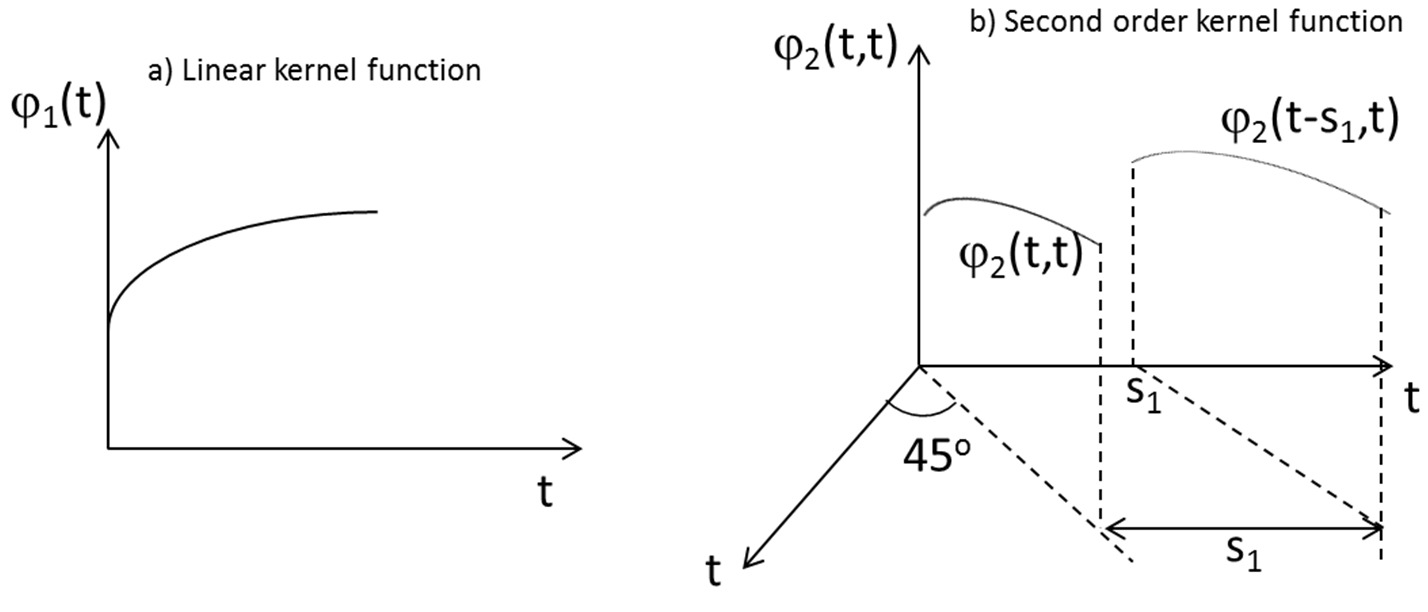
\includegraphics[width=5.0in]{./chap_3_minor_loop/figures/Time_dependent_kernel_functions.png}
\caption{The comparison between viscoelastic and elastic materials as host structure.}
\label{fig:2.1.Time_dependent_kernel_functions}
\end{figure}
 

\begin{figure} 
\centering 
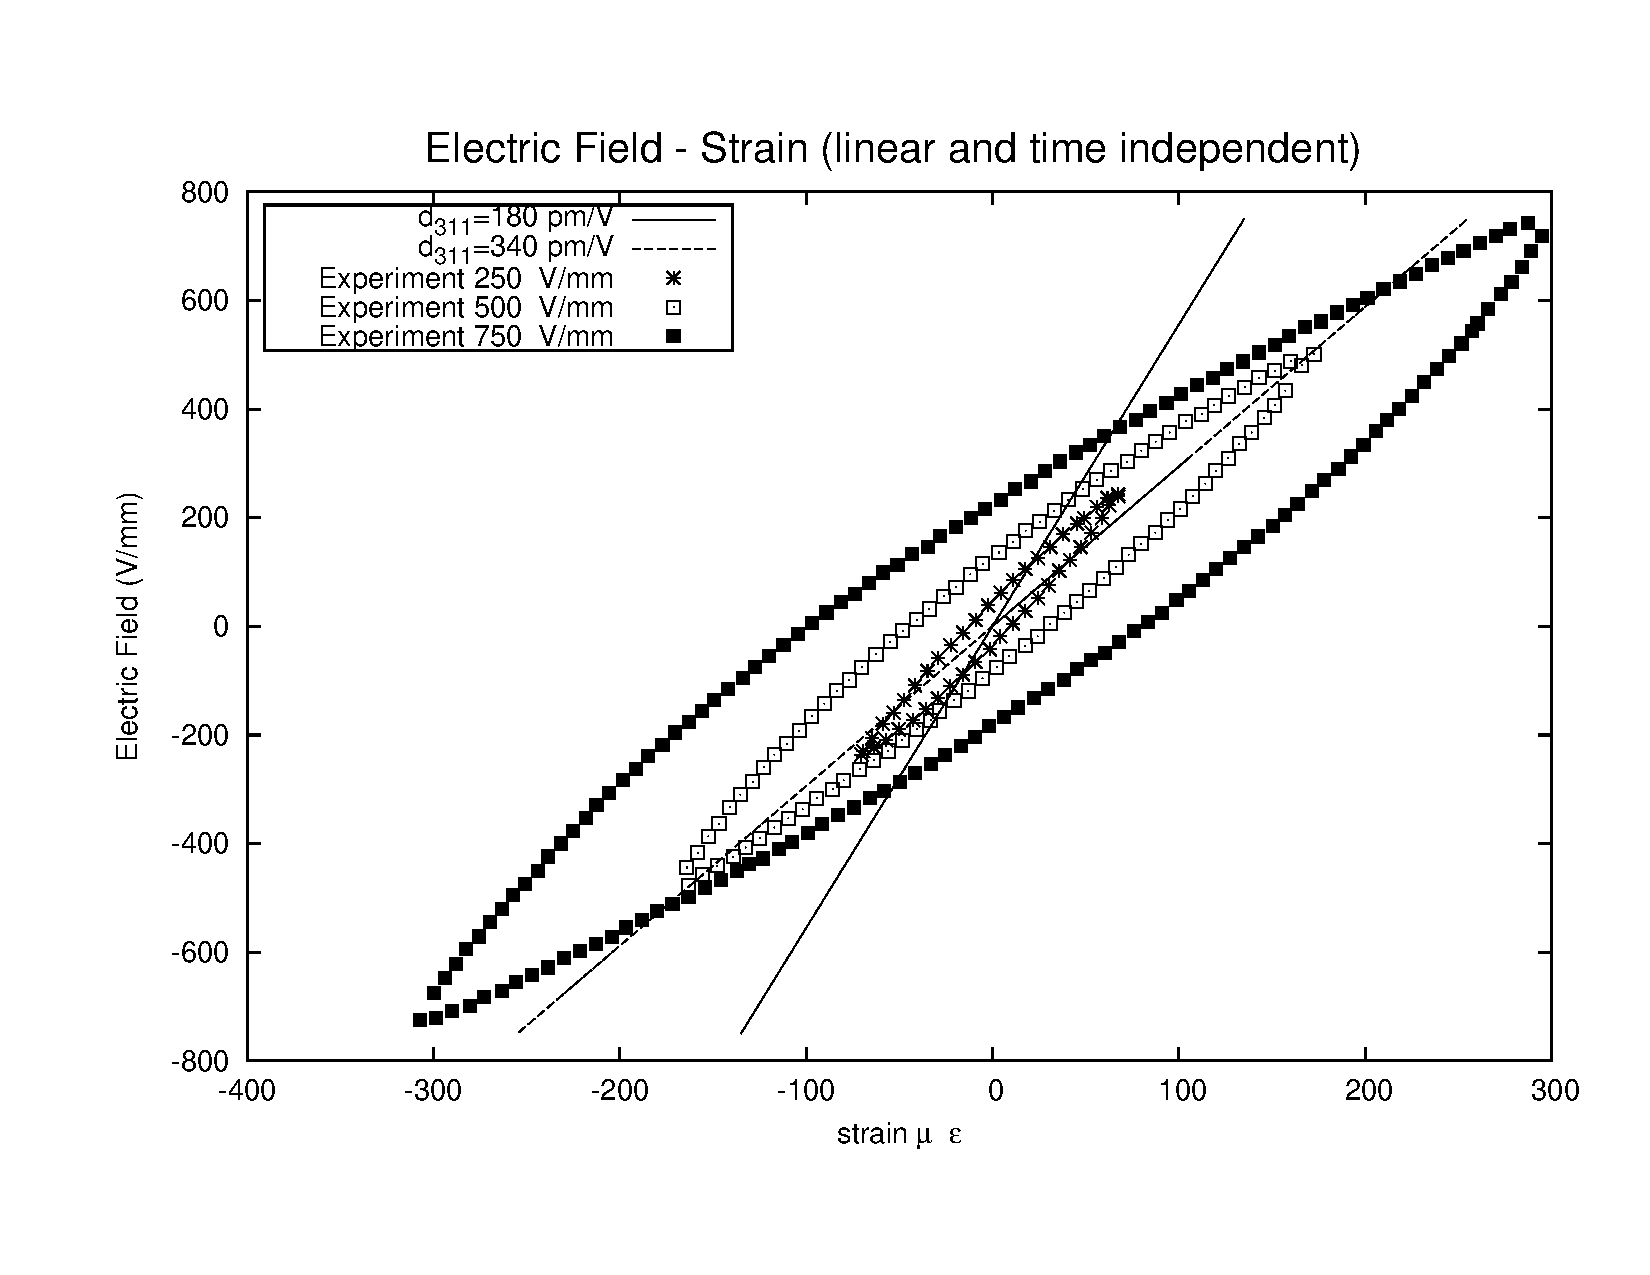
\includegraphics[width=5.0in]{./chap_3_minor_loop/figures/crawley_linear_time_independent.pdf}
\caption{Linear time independent model compared with experimental strain ($\varepsilon_{11}$) response under electric field ($E_3$) with frequency 0.1 Hz in \cite{Crawley1990}.}
\label{fig:Crawley_xp_TimeinDepenLin}
\end{figure}
 
\begin{figure} 
\centering
\includegraphics[width=5.0in]{./chap_3_minor_loop/figures/crawley_linear_time_dependent-eps-converted-to.pdf}
\caption{Linear and history dependent model compared with experimental strain ($\varepsilon_{11}$) response under electric field ($E_3$) with frequency 0.1 Hz in \cite{Crawley1990}.}
\label{fig:Crawley_xp_His_dependent_Lin}
\end{figure}
  
\begin{figure}
\centering
\includegraphics[width=5.0in]
{./chap_3_minor_loop/figures/crawley_non_linear_time_dependent-eps-converted-to.pdf}
\caption{Nonlinear time dependent strain ($\varepsilon_{11}$) response under electric field ($E_3$) with frequency 0.1 Hz compared with experiment\cite{Crawley1990}.}
\label{fig:TimeDepenNonLinCrawley}
\end{figure}

\begin{figure}
\centering
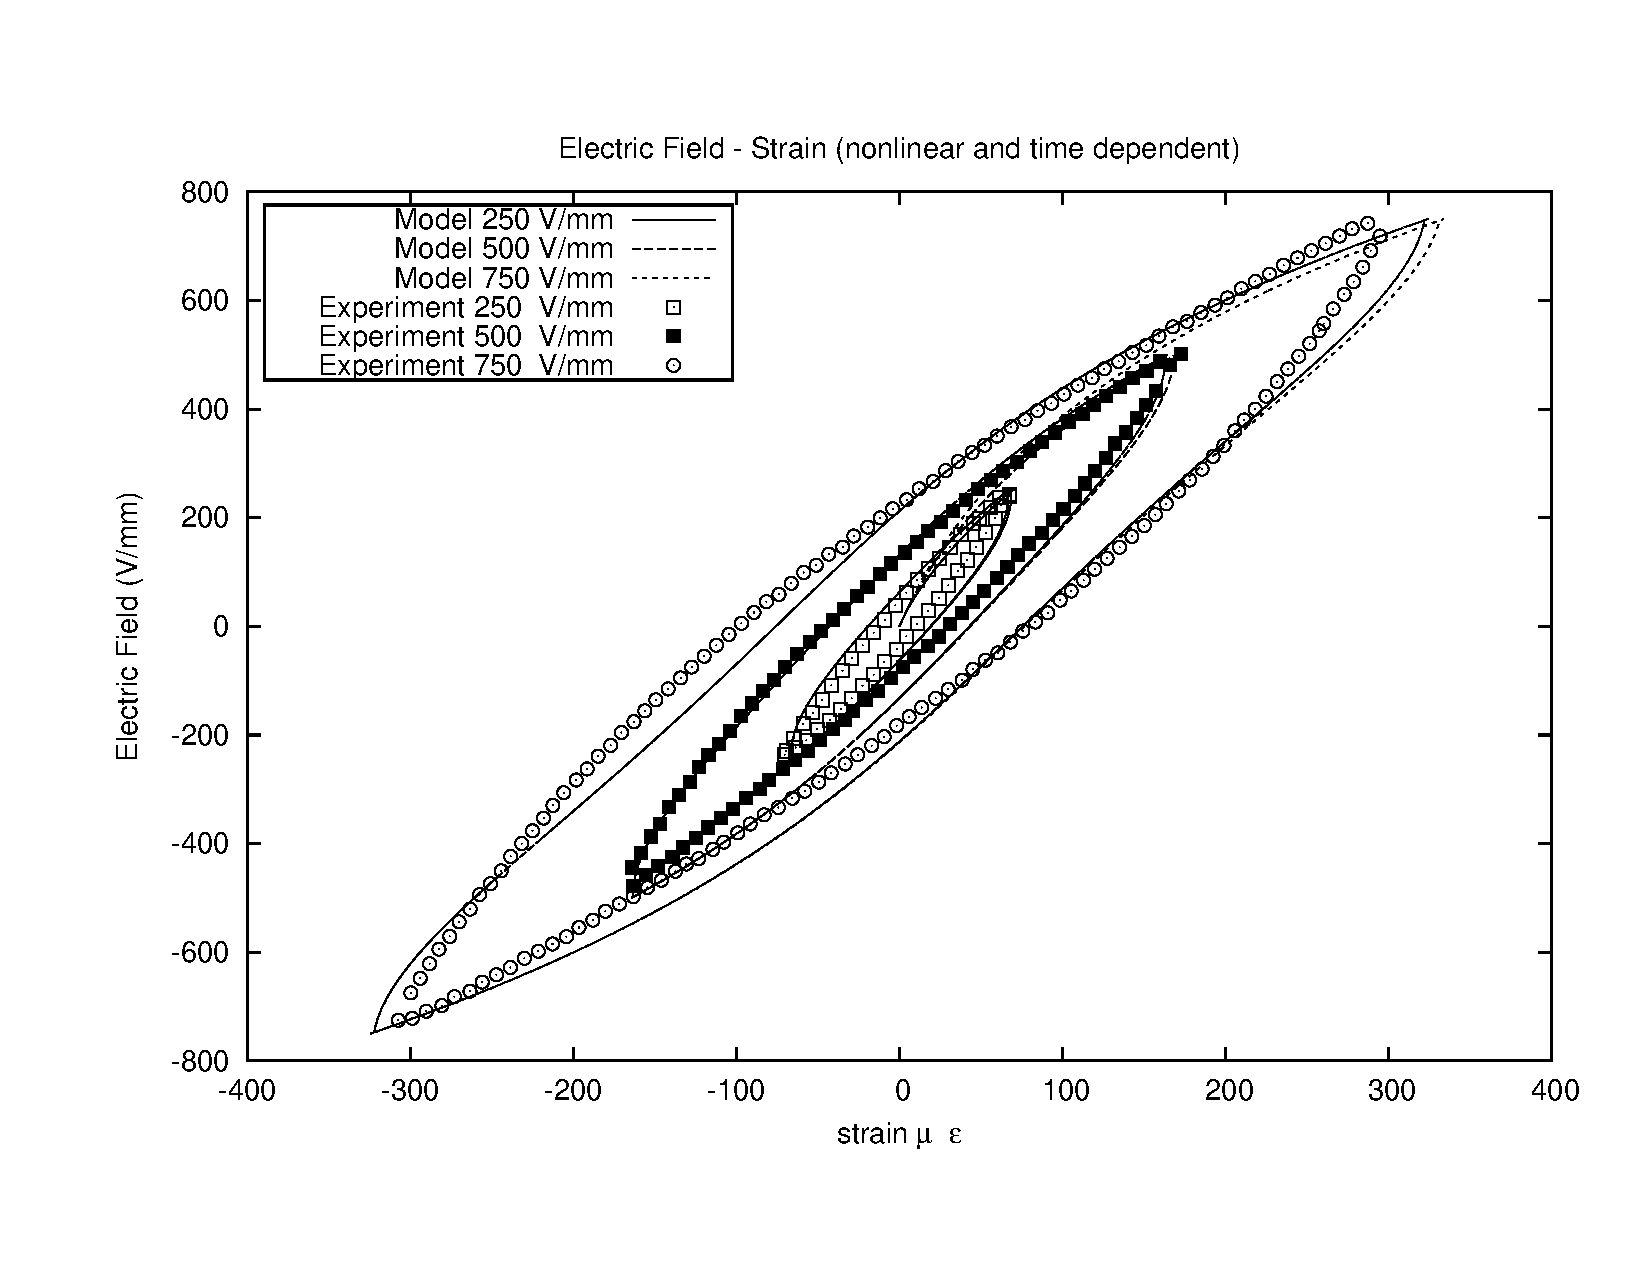
\includegraphics[width=5.0in]
{./chap_3_minor_loop/figures/crawley_non_linear_time_independent_third_order.pdf}
\caption{Nonlinear time dependent strain ($\varepsilon_{11}$) response under electric field ($E_3$) with frequency 0.1 Hz for third order model compared with experiment\cite{Crawley1990}.}
\label{fig:TimeDepenNonLinCrawleyThirdordermodel}
\end{figure}


\begin{figure}
\centering
\includegraphics[width=5.0in]
{./chap_3_minor_loop/figures/crawley_non_linear_time_dependent_frequency_effect-eps-converted-to.pdf}
\caption{Effect of frequency of applied electric field ($E_3$) on strain ($\varepsilon_{11}$) response.}
\label{fig:Frequency_Effect}
\end{figure}

\begin{figure}
\centering
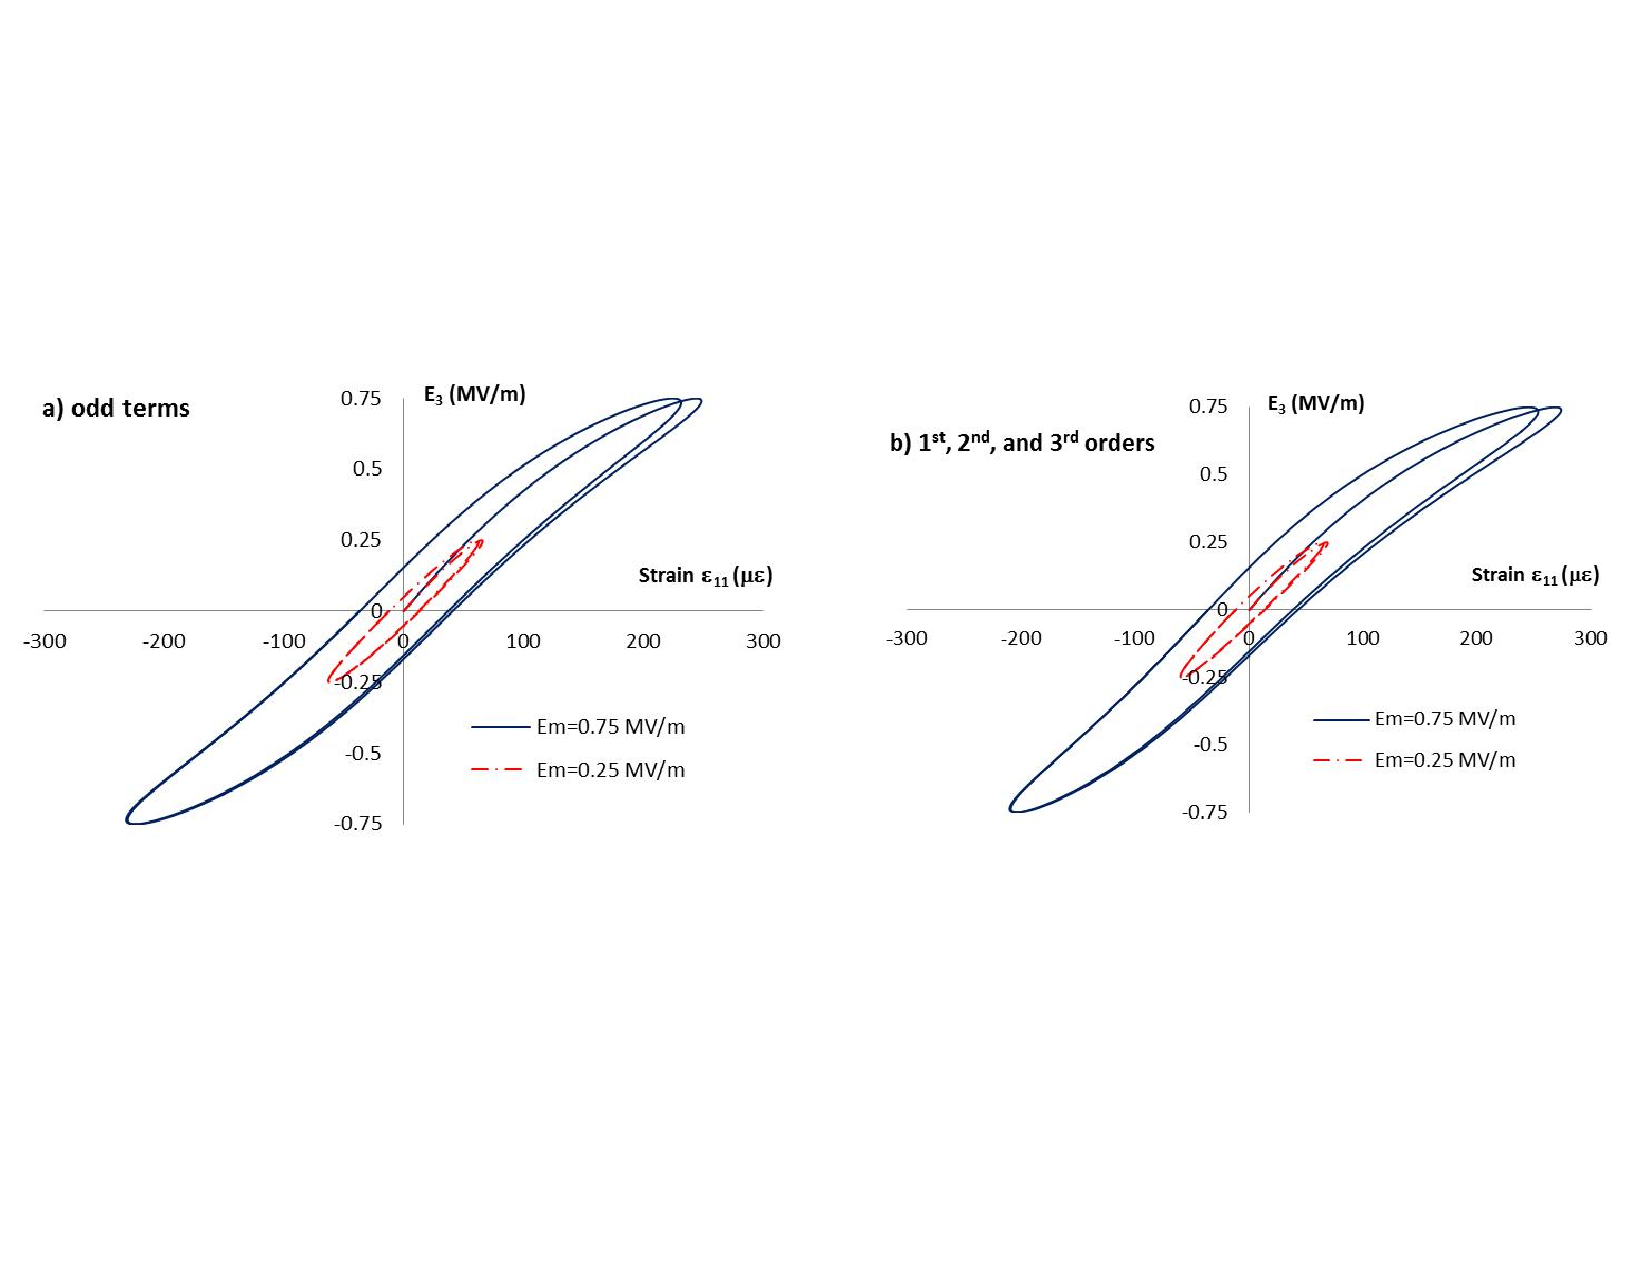
\includegraphics[width=5.0in]
{./chap_3_minor_loop/figures/figure_3_8_the_effect_of_the_higher_order_terms_on_the_hysteretic_response.pdf}
\caption{The effect of the higher order terms on the hysteretic response (f=0.1 Hz)}
\label{figure_3_8_the_effect_of_the_higher_order_terms_on_the_hysteretic_response}
\end{figure}

\begin{figure}
\centering
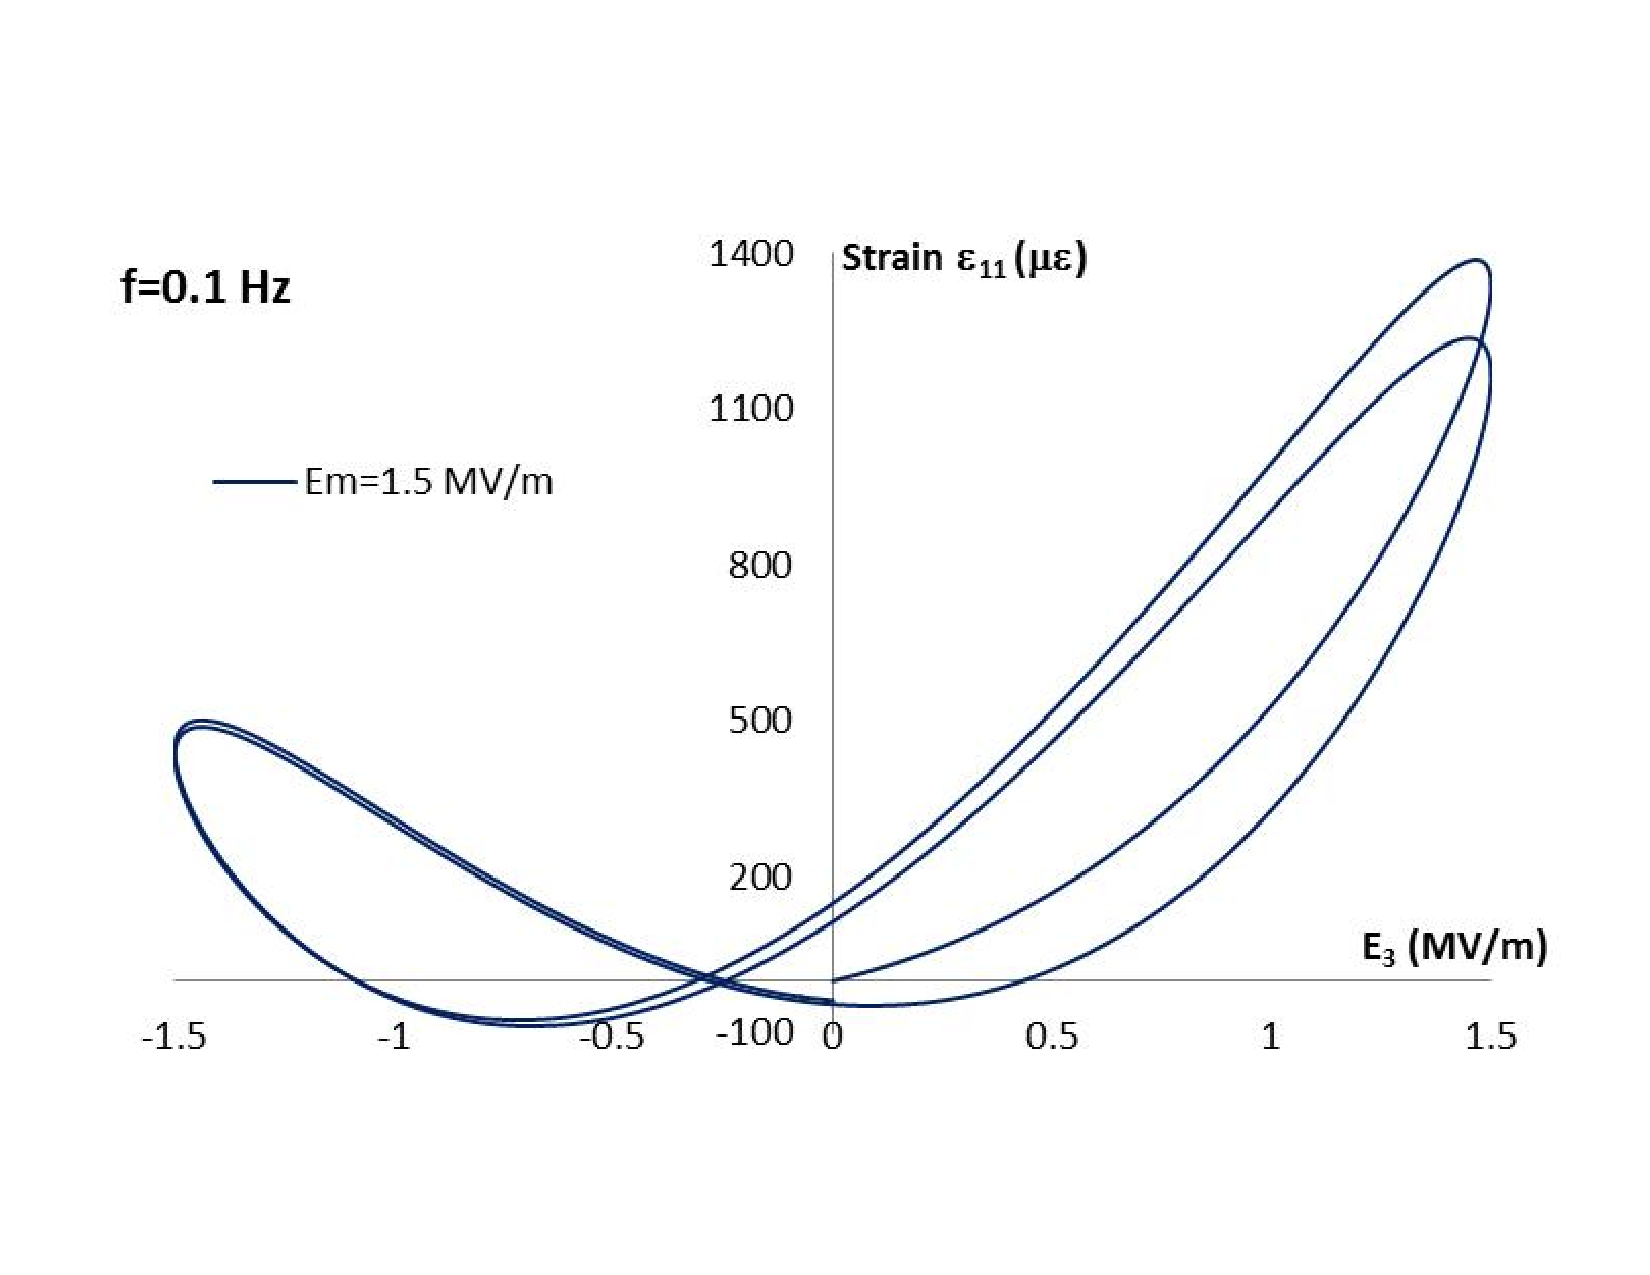
\includegraphics[width=5.0in]
{./chap_3_minor_loop/figures/fig_3_9_the_butterfly-like_shape_of_the_electro-mechanical_coupling_response.pdf}
\caption{The butterfly-like shape of the electro-mechanical coupling response}
\label{fig_3_9_the_butterfly-like_shape_of_the_electro-mechanical_coupling_response}
\end{figure}


\begin{figure}
\centering
\includegraphics[width=1.0in]{./chap_3_minor_loop/figures/PZT_586_Geometry-eps-converted-to.pdf}
\caption{Geometry of PZT-586 Telescopic Actuator (dimensions are in mm)}
\label{fig:Geometry_PZT-586}
\end{figure}


\begin{figure}
\centering
\includegraphics[width=5.0in]{./chap_3_minor_loop/figures/telescopic_actuator_pztl_586_elec_pot_deflection_uy-eps-converted-to.pdf}
\caption{Electric potential and deflection contour of PZT-586 Telescopic Actuator}
\label{fig:PZT-586_response}
\end{figure}

\begin{figure}
\centering
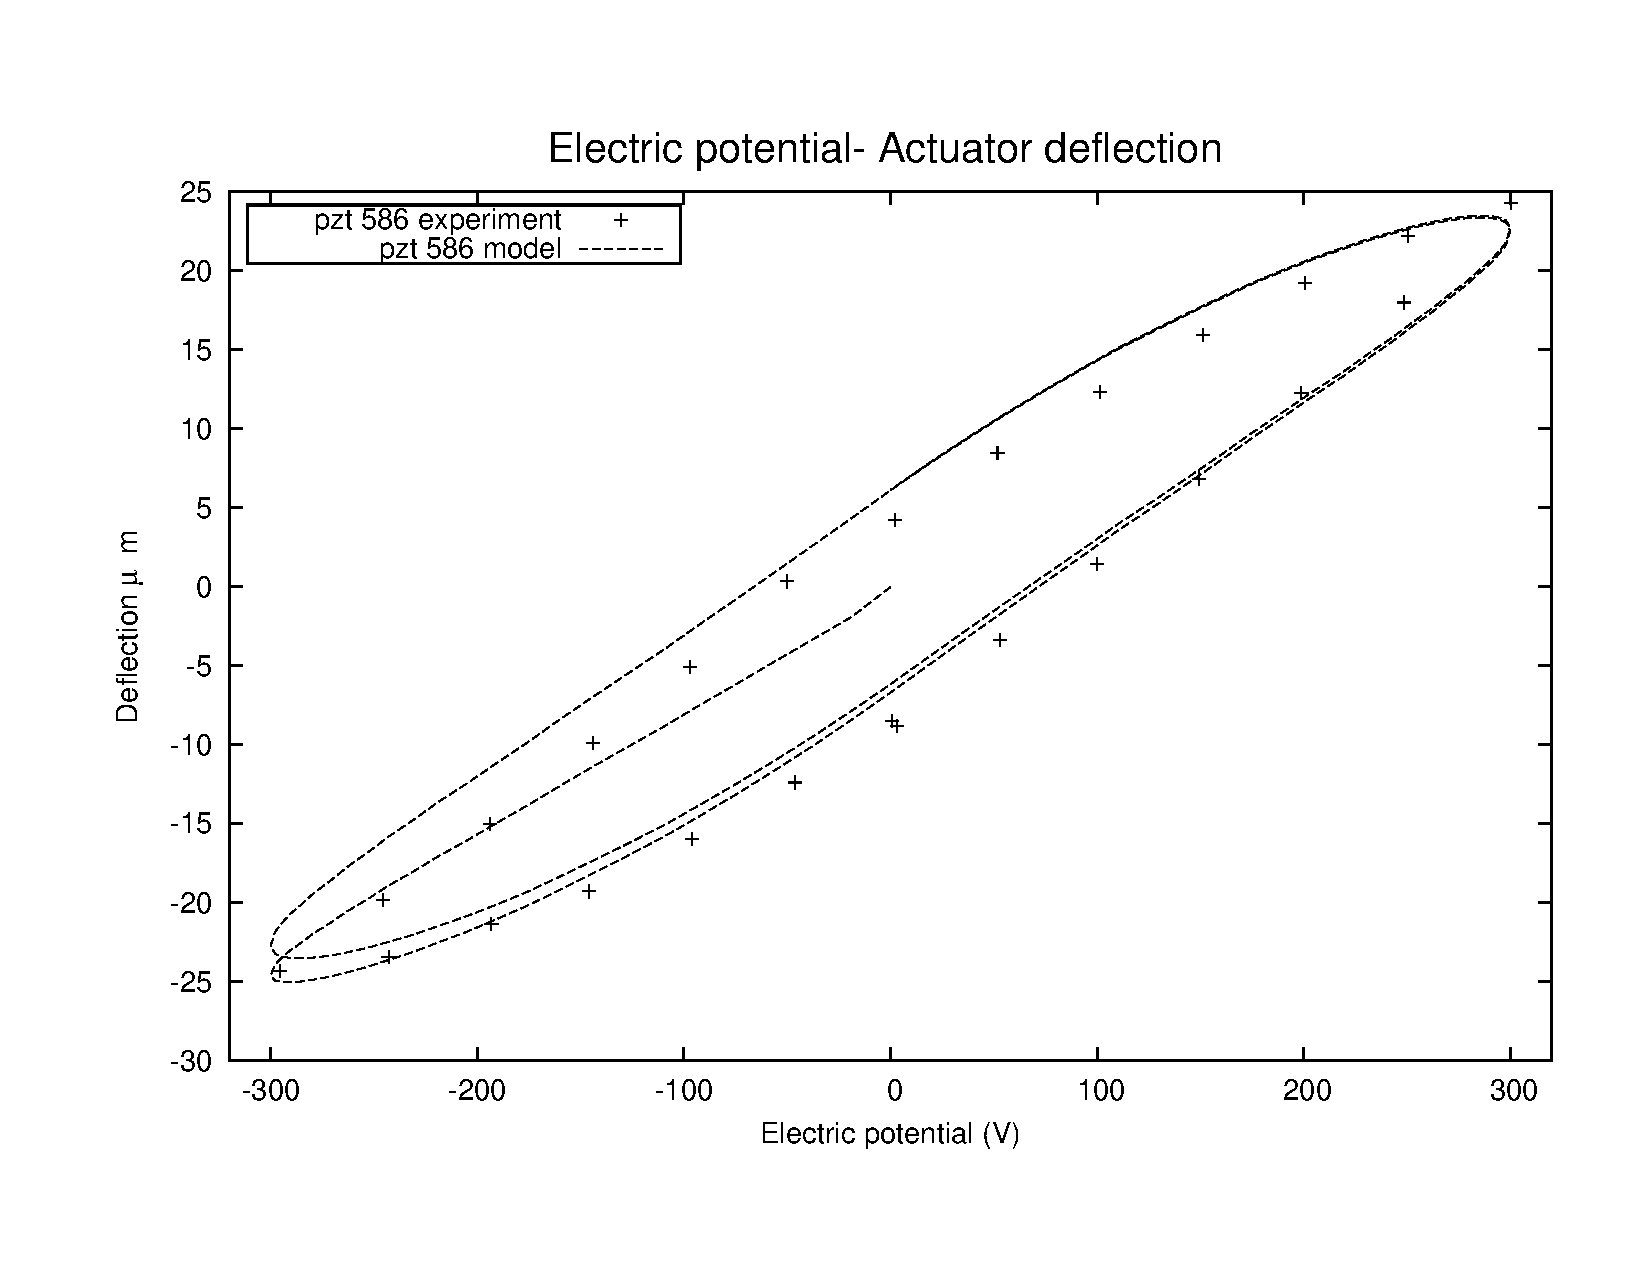
\includegraphics[width=5.0in]{./chap_3_minor_loop/figures/result_pzt_586.pdf}
\caption{Tip deflection of PZT-586 comparing FEM with experiment}
\label{fig:PZT_586_XP_Calib}
\end{figure}

\begin{figure}
\centering
\includegraphics[width=3.0in]{./chap_3_minor_loop/figures/MSI_53_XP_Geometry-eps-converted-to.pdf}
\caption{Geometry of MSI-53 (dimensions are in mm)}
\label{fig:MSI_53_Geometry}
\end{figure}


\begin{figure}
\centering
\includegraphics[width=5.0in]{./chap_3_minor_loop/figures/telescopic_actuator_msi_53_elec_pot_deflection_uy-eps-converted-to.pdf}
\caption{Geometry of MSI-53}   
\label{fig:MSI_53_XP_contour}  
\end{figure}
 

\begin{figure}
\centering
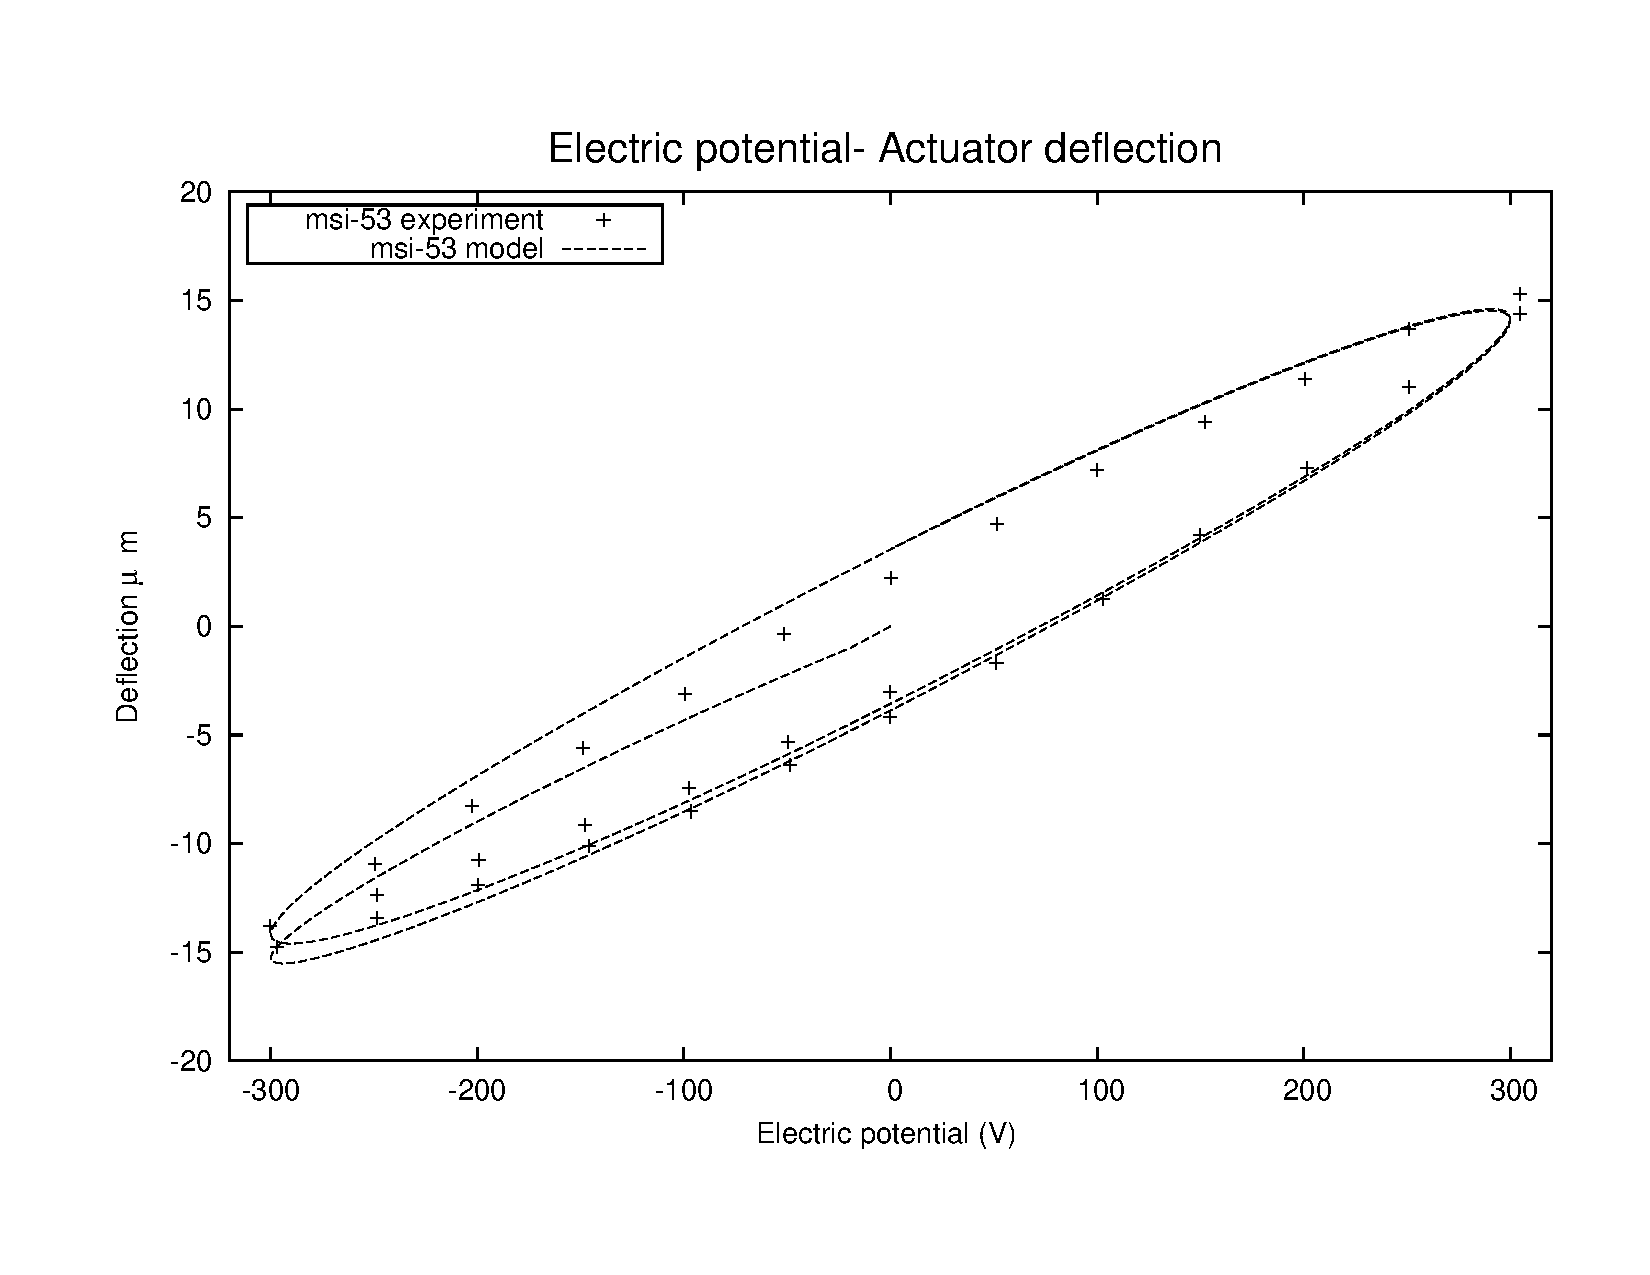
\includegraphics[width=5.0in]{./chap_3_minor_loop/figures/result_msi-53.pdf}
\caption{Tip deflection of MSI-53 comparing FEM model with experiment}
\label{fig:MSI_53_XP_results}
\end{figure}
% %%%%%%%%%%%%%%%%%%%%%%%%%%%%%%%%%%%%%%%%%%%%%%%%%%%
%
%  New template code for TAMU Theses and Dissertations starting Fall 2012.  
%  For more info about this template or the 
%  TAMU LaTeX User's Group, see http://www.howdy.me/.
%
%  Author: Wendy Lynn Turner 
%	 Version 1.0 
%  Last updated 8/5/2012 
%
%%%%%%%%%%%%%%%%%%%%%%%%%%%%%%%%%%%%%%%%%%%%%%%%%%%  
%%%%%%%%%%%%%%%%%%%%%%%%%%%%%%%%%%%%%%%%%%%%%%%%%%%%%%%%%%%%%%%%%%%%%%
%%                           SECTION III
%%%%%%%%%%%%%%%%%%%%%%%%%%%%%%%%%%%%%%%%%%%%%%%%%%%%%%%%%%%%%%%%%%%%%
\chapter{\uppercase{STRUCTURAL ANALYSES}}  
\label{section:structural_analyses}
This chapter presents analyses of electro-active structures under several loading histories.
The constitutive equations that were introduced in the previous chapters are used for the active materials.
Two types of smart structures are studied, which are smart multi-layered beams and active fiber composites.
The smart beams consist of layers of piezoelectric and inactive materials.
Through thickness electric fields are prescribed in order to create bending in the beams.
Analytical solutions of the deflections of smart beams with time dependent and electro-mechanical coupling effect are presented.
The analytical solutions are also compared to the results obtained from finite element analyses and experiments.
The active fiber composite comprises of unidirectional fibers placed in a polymeric matrix.
Electrode fingers are attached to the top and bottom surfaces of the composite.
In this study, a representative unit cell model is considered for the active fiber composite and the overall electro-mechanical response of the composite is examined. \\

\section{Analyses of Smart Beams}
Analytical and numerical solutions of the time-dependent electro-mechanical coupled deformations of piezoelectric multi-layered composite beams are presented. 
The Laplace transform method is used to obtain the analytical solutions while finite element method is considered for the numerical solutions.
The results from the analytical solutions are compared with the experimental data and finite element solutions.
Several parametric studies are also conducted in order to study the time-dependent electro-mechanical behavior of the composites.

\begin{figure}
\centering
\includegraphics[width=6.0in]{./chap_4_structural_analyses/pdf_beam/PVDF_beam_geometry.pdf}
\caption{Substrated bimorph beam geometry}
\label{fig:PVDF_beam_geometry}
\end{figure}

\subsection{Governing Equation for Electro-Active Beams}
The analyses presented here are suitable for multi-layered slender beams undergoing small deformation gradients.
Figure \ref{fig:PVDF_beam_geometry} illustrates an example of a multi-layered active beam.
This beam has three layers, two active layers at the top and bottom and one substrate (inactive) layer in the center.
There are electrodes on the surfaces of active layer.
An electric field is obtained to these active layers by applying an electric potential difference to the electrodes.
In order to describe the various beam theories, the following coordinate system is introduced.
The
 $x_1$-coordinate is taken along the length of the beam,
 $x_2$-coordinate is taken along the width of the beam, and the
 $x_3$-coordinate along the thickness (the height) of the beam.
According to this coordinate system the loading and geometry are such that the displacements
 $(\bar {u_1}, \bar {u_2}, \bar {u_3})$ along the coordinates axis
 $( {x_1}, {x_2},  {x_3})$ are independent of $x_2$.
Moreover, it is assumed that displacements in the width of the beam $\bar {u_2}$ is zero.
For the beam analyses, the field variables are:
stress $\sigma_{11}$ and
strain $\varepsilon_{11}$ along the longitudinal axis of the beam,
electric field $E_3$ and electric flux (displacement) $D_3$ through the thickness of the beam.
Strain and electric field are taken as the independent variables.
The corresponding stress and electric displacement field for a linear electro-mechanical response is expressed as:

\begin{equation}
\begin{aligned}
&\sigma_{11}=C_{1111} \varepsilon_{11}-e_{311} E_{3} \\
&D_3=e_{311} \varepsilon_{11}+\kappa_{33}^\varepsilon E_{3}
\end{aligned}
\label{stress_1D_const_eqn_beam:EQN}
\end{equation}
where $C_{1111}$ is the elastic stiffness measured at constant electric field,
$e_{311}$ is the piezoelectric constant, and $\kappa_{33}^\varepsilon$ is the dielectric coefficient at constant strain.

The above constitutive model is used for the static response of piezoelectric material.
This study deals with time dependent response of active composite beams with nonlinear electro-mechanical behavior.
The following constitutive relations for the time-dependent-electro-elastic deformation of solids
 (see chapter \ref{section:minor_loop_constitutive_model_for_polarized_piezo_electric}) is used for the piezoelectric composite beams shown in figure \ref{fig:PVDF_beam_geometry}:

\begin{equation}
\begin{aligned}
\sigma_{11}(t)=
&\int_{0^-}^t
K^C(t-s)\frac{\partial \sigma_{11}}{\partial\varepsilon_{11}} (\varepsilon_{11}(s))\frac{\partial {\varepsilon}_{11}(s)}  {\partial s} ds +\\
&\int_{0^-}^t
K^e (t-s) \frac{\partial \sigma_{11}}{\partial E_{3}}(E_3(s))  \frac{\partial {E}_{3} (s)}  {\partial s} ds
\\
D_3(t)=
&\int_{0^-}^t
K^{e}(t-s)
\frac{\partial D_{3}}{\partial \varepsilon_{11}}(\varepsilon_{11}(s))
\frac{ \partial {\varepsilon}_{11}(s)}  {\partial s}  ds + \\
&\int_{0^-}^t
K^{\kappa}(t-s) \frac{\partial D_{3}}{\partial E_{3}}(E_3(s))  \frac{\partial {E}_{3} (s)}  {\partial s} ds
\end{aligned}
\label{visco_stress_1D_const_eqn_beam:EQN}
\end{equation}
This is a one dimensional version of the 3D constitutive equation that is suitable for beam analyses.
$K^{\kappa}(t), K^e(t), K^C(t)$ are the normalized time dependent kernels.
The time kernels in this constitutive equation can be expressed in terms of Prony series as discussed in chapter \ref{section:minor_loop_constitutive_model_for_polarized_piezo_electric}. 
A beam is defined as a structural element that is predominantly under bending. 
Three beam theories are considered which are the classical Euler-Bernoulli beam theory, Timoshenko beam theory, and higher order beam theory.
The Euler-Bernoulli beam theory is followed, in which the deformation due to the transverse shear is ignored.
The displacements fields are defined in terms of only two unknown variables, for the transverse displacement and axial displacement:

\begin{equation}
\begin{aligned}
& \bar {u_1} (x_1,x_2,x_3,t)=u_1 (x_1,t)-x_3  \frac{\partial u_3 (x_1,t)} {\partial x_1} \\
& \bar {u_2} (x_1,x_2,x_3,t)=0 \\
& \bar {u_3} (x_1,x_2,x_3,t)=u_3 (x_1,t)
\end{aligned}
\label{eluer_beam:EQN}
\end{equation}
where  $(u_1,u_3)$ are the displacements along the coordinates axis $({x_1}, {x_3})$ measured at the neutral axis.
The Euler-Bernoulli beam theory is valid when the beams are slender enough.
On the other hand if the shear stress in the thickness direction of the beam contributes to the lateral deflection, Timoshenko beam theory is used.
The Timoshenko beam theory assumes a constant shear stress in the thickness of beam and the normal axis to the neutral axis of the beam can rotate with respect to the center line.
This will introduce a new degree of freedom and a new unknown function due to the additional rotation:

\begin{equation}
\begin{aligned}
& \bar {u_1} (x_1,x_2,x_3,t)=u_1 (x_1,t)+x_3  \psi_2(x_1,t)  \\
& \bar {u_2} (x_1,x_2,x_3,t)=0 \\
& \bar {u_3} (x_1,x_2,x_3,t)=u_3 (x_1,t)
\end{aligned}
\label{timoshenko_beam:EQN}
\end{equation}

In the Timoshenko beam theory, the unknown function $\psi_2(x_1,t)$ is a measure of rotation of the beam.
The axial beam displacement ${u_1}$ and transverse displacement field of the beam ${u_3}$ have the same meaning as equation (\ref{eluer_beam:EQN}).
It can be shown by the elasticity solution that the through thickness stress of the beam is quadratic with respect to the transverse coordinate $x_3$ while the Timoshenko beam theory assumes a constant shear stress through the thickness.
In order to correct this inconsistency the shear energy of beam is related to the shear energy of the Timoshenko beam by a constant called shear correction factor.
This constant depends on the geometry of the cross section of the beam and it affects the accuracy of the solutions.
The higher order beam theory is introduced to account for the quadratic distribution of the shear through the thickness of the beam and relax the need for the shear correction factor.


The higher order beam theory uses the same number of degrees of freedom as the Timoshenko beam and therefore, the same number of unknowns of the displacement field.
Using the fact that, the shear stress is zero in the upper and bottom surface of the beam, the quadratic distribution of the shear stress in the thickness is defined.
The displacement field of the theory is defined based on three unknown as in the Timoshenko beam theory:

\begin{equation}
\begin{aligned}
& \bar {u_1} (x_1,x_2,x_3,t)=u_1 (x_1,t)+x_3  \phi_2(x_1,t) +\alpha x_3^3(\phi_2(x_1,t)+\frac{\partial u_3 (x_1,t)} {\partial x_1}) \\
& \bar {u_2} (x_1,x_2,x_3,t)=0 \\
& \bar {u_3} (x_1,x_2,x_3,t)=u_3 (x_1,t)
\end{aligned}
\label{higher_order_beam:EQN}
\end{equation}

By applying stress free conditions on the top and bottom surface of the beam value of $\alpha$ is found to be  $-4/(3h^2)$ \cite{Wang2000}.
Here $\phi_2(x_1,t)$ is defined as the slope of the normal line measured from the neutral axis.
It can be seen that the normal line in the beam is not straight anymore and it is defined as a cubic function.
The non zero strain component for the displacement defined in the beam equations (\ref{eluer_beam:EQN}-\ref{higher_order_beam:EQN}) are:
\begin{equation}
\begin{aligned}
& \varepsilon_{11} (x_1,x_3,t)=\frac{\partial    \bar {u_1} (x_1,x_3,t) } {\partial x_1} - x_3 \frac{\partial^2 \bar{ u_3} (x_1,x_3,t) } {\partial x_1^2} \\
& 2  \varepsilon_{13} (x_1,x_3,t)=\frac{\partial \bar {u_3} (x_1,x_3,t) } {\partial x_1} + \frac{\partial       \bar{ u_1} (x_1,x_3,t)} {\partial x_3}
\end{aligned}
\label{_strain_beam:EQN}
\end{equation}
This strain formulation can be used for each of the above beam theories.
It is worth noting that for the Euler-Bernoulli beams theory $\varepsilon_{13}$ is zero.
The higher order beam theories can incorporate the effect of shear in the thickness of the beam.
In the case of active composite beams are subjected to electric field through thickness with no transverse mechanical loading, the transverse shear deformation is insignificant.
As a result, using the Timoshenko or higher order beam theories for predicting the deflection gives the same result as the Euler-Bernoulli beam theory.
Therefore, in this study the Euler-Bernoulli beam theory is used for for the smart beams.



Using the variational method, the equilibrium equations for the beam model are determined.
The external axial force $N_{11} (x_1,t)$ and bending moment  $M_{11} (x_1,t)$ are given as:

\begin{equation}
\begin{aligned}
& N_{11} (x_1,t)=\int_{x_2,x_3}\sigma_{11} (x_1,x_3,t)dx_2 dx_3 \\
& M_{11} (x_1,t)=\int_{x_2,x_3}x_3 \sigma_{11} (x_1,x_3,t)dx_2 dx_3 \\
\end{aligned}
\label{resultant_strain_beam:EQN}
\end{equation}
The equilibrium equations for the beam bending are:

\begin{equation}
\begin{aligned}
& \frac{\partial N_{11} (x_1,t)}{\partial x_1}=f(x_1,t) \\
& -\frac{\partial^2 M_{11} (x_1,t)}{ \partial x^2_1}=q(x_1,t)\\
\end{aligned}
\label{equilibrium_resultant_strain_beam:EQN}
\end{equation}
where
$f(x_1,t)$ and $q(x_1,t)$  are  the
distributed axial and transverse loads respectively.

\subsection{Responses of 3-Layered Active Beam Under Constant Electric Field}
\label{section:piezo_beam_static_elastic_solution}
This section presents solution for the analyses of 3-layered active beams using the Euler-Bernoulli beam theory.
First, the response of the beam neglecting the time dependent effect is obtained.
This result is used to verify the finite element formulation and also used to develop the time dependent solution by using the Laplace transform method.
The analytical method that is discussed here is then extended to time dependent and nonlinear electro-mechanical formulation.


Consider a bimorph beam with a thickness $h$ as shown in figure \ref{fig:PVDF_beam_geometry}.
The beam consists of two layers of piezoelectric materials with thickness $h_p/2$ each.
A substrate layer between these two layers of piezoelectric has a thickness $h_s$.
In practice there are electrodes placed between layers and also on the top and bottom parts of the beam in order to prescribe electric field inputs.
If the electric potential $V$ is applied to top and bottom electrodes, the
 piezoelectric layers will be subjected to electric field $E_3=2V/h_p$.
The applied electric field in each layer can be either positive or negative depending on the direction of electric potential applied.
Regardless of the sign of the applied potential the direction of the formed electric fields on the top and bottom layers are opposite to each other in order to create bending.
Since the electrode layer is very thin, its effect on the overall response of the beam is disregarded.
The total thickness of the beam is $h=h_p+h_s$ as shown in figure \ref{fig:PVDF_beam_geometry}. 
Using the equilibrium equation in (\ref{equilibrium_resultant_strain_beam:EQN}), and the linear electro-mechanical constitutive model
 presented in equation (\ref{stress_1D_const_eqn_beam:EQN}) the axial force and bending moments are:

\begin{equation}
\begin{aligned}
 N_{11} (x_1)=& \left( w{\it C_p} {\it h_p}+w{\it C_s} {\it h_s} \right) {\it u_1} \\
 M_{11} (x_1)=& \left( -  {  C_p} {{  h_p}}^{2}{  h_s}/4- {C_p}
{h_p} {{  h_s}}^{2}/4- {C_p} h_p^3/12- { C_s} {{h_s}}^{3} /12 \right)w
\frac{\partial^2 u_3 (x_1,t)} {\partial x_1^2}-  \\
& w e E_3 ( {h_p} {h_s}/2- {h_p}^{2}/4)
\end{aligned}
\label{EQN:stress_resultant_integration_definistion}
\end{equation}
where
$w$ is the width of the beam.
A simplified notation for the material parameters is considered here.
For the piezoelectric layer the stiffness and piezoelectric constants are $C_{1111}=C_p$, $e_{311}=e$ respectively.
For the elastic substrate the properties are $C_{1111}=C_s$ and $e_{311}=0$.
The effect of the electric displacement on the strain is ignored.
If the beam shown in figure \ref{fig:PVDF_beam_geometry} is clamped at the left end, the boundary conditions are as follows:
\begin{equation}
u_1(0)=u_3(0) =\frac{ \partial u_3(0) } {\partial x_1}=0
\label{Eqn:clamped_beam_boundary_conditions}
\end{equation}
Then, for a beam with no transverse loading the deflection of the beam is:
\begin{equation}
u_3
(x_1)=\frac{1}{2}\frac{3 e E h_p (h_p+2h_s)}{C_p h_p^3+3
C_p h_p^2 h_s+3C_p h_p h_s^2+C_s h_s^3} x_1^2
\label{EQN:deflecction} 
\end{equation}


The above analyses is extended for the time dependent constitutive equation of active composite beams.
The time dependent electro-mechanical constitutive piezoelectric layers and linear visco-elasticity is considered for the substrate.
A closed-form solution for the deformations of the active beam is presented.
The time dependent response of the beam is obtained by using the Laplace transform method.
Consider the beam geometry as shown in figure \ref{fig:PVDF_beam_geometry},
 with the constitutive equation (\ref{visco_stress_1D_const_eqn_beam:EQN}) for the piezoelectric layers of the beam.
The stress in the piezoelectric layers is additively decomposed into the mechanical and electro-mechanical stresses:
\begin{equation}
\sigma_{11}=\sigma_{11}^m+\sigma_{11}^e
\end{equation}
where
\begin{equation}
\begin{aligned}
\sigma_{11}^m&=\int_{0^-}^t
K^C(t-s)\frac{\partial \sigma_{11}}{\partial\varepsilon_{11}} (\varepsilon_{11}(s))  \frac{\partial {\varepsilon}_{11}(s)}{\partial s}ds\\
\sigma_{11}^e&=\int_{0^-}^t
K^e (t-s) \frac{\partial \sigma_{11}}{\partial E_{3}}(E_3(s)) \frac{\partial {E}_{3} (s)}{\partial s} ds
\end{aligned}
\label{eqn:history_dependent_stress_and_strain}
\end{equation}

The mechanical stress is considered to be linear and elastic,
which for the host structure and active layer are $\sigma_{11}^m=C_s \varepsilon_{11}$ and $\sigma_{11}^m=C_p \varepsilon_{11}$.
The stress due to the electro-mechanical coupling is defined as a polynomial function of the electric field in order to include the effect of high electric fields.



The Laplace transform is used to transform the equations from time domain to the Laplace variable domain.
The derivatives with respect to time will be expressed as polynomials with respect to the Laplace variable.
The constitutive equation (\ref{eqn:history_dependent_stress_and_strain}) for beam is presented in the Laplace form as:

\begin{equation}
\mathcal{L} \left[ \sigma_{11}(t) \right]=a  C_p \mathcal{L} \left[ K^C(t) \right] \mathcal{L} \left[ \varepsilon_{11}(t) \right]
\end{equation}
where $\mathcal{L}$ is the Laplace transform and $a$ is the transform variable.
In the same manner the Laplace transform for the electro-mechanical stress $\sigma_{11}^e$ is defined.

\begin{equation}
\mathcal{L} \left[ \sigma_{11}^e(t) \right]=\mathcal{L} \left[
\int_{0^-}^t
K^e (t-s) \frac{\partial \sigma_{11}}{\partial E_{3}}(E_3(s))  \dot{E}_{3} (s)ds
\right]
\label{EQN:Laplace_stress_coupling}
\end{equation}
Since the electric field is known, the explicit definition of the electro-mechanical coupling stress in the Laplace domain is obtained using equation (\ref{EQN:Laplace_stress_coupling}).
The Laplace transform turns the time dependent integral equation into an algebraic equation.


% In dealing with nonlinear and time dependent response we are dealing a differential equation for displacement field with respect to coordinates and also integral equation with respect to time.
% Laplace transform will seperate the time dependent integral equation and turn it into polynomila with respect to laplace variable so we can solve the ordinary equation with respect to coordinate such as static case.
The differential equation for the displacement with respect to spatial variables are given in equations (\ref{equilibrium_resultant_strain_beam:EQN}) and (\ref{resultant_strain_beam:EQN}).
The axial force and bending moment in the Laplace domain are:

\begin{equation}
\begin{aligned}
&\bar{N}_{11} (x_1,a)=\int_{x_2,x_3} \bar{\sigma}_{11} (x_1,x_3,a) dx_2 dx_3 \\
&\bar{M}_{11} (x_1,a)=\int_{x_2,x_3} x_3 \bar{ \sigma}_{11} (x_1,x_3,a) dx_2 dx_3 \\
\end{aligned}
\label{EQN:laplac_resultant_strain_beam}
\end{equation}
where the upper bar means the function in Laplace domain.
The equilibrium equations are:

\begin{equation}
\begin{aligned}
& \frac{\partial \bar{N}_{11} (x_1,a)}{\partial x_1}=\bar{f}(x_1,a) \\
& -\frac{\partial^2 \bar{M}_{11} (x_1,a)}{ \partial x^2_1}=\bar{q}(x_1,a)\\
\end{aligned}
\label{EQn:Laplace_equilibrium_resultant_strain_beam}
\end{equation}
It is noted that the applied transverse and axial boundary conditions should be defined in the Laplace domain.
The Laplace transform should also be performed for the time dependent boundary conditions.
Solving the differential equations presented in equation (\ref{EQn:Laplace_equilibrium_resultant_strain_beam}) will result in transverse deflection in Laplace space $\bar{u}_3(x_3,a)$.
The inverse of the Laplace transform gives the function in time domain:

\begin{equation}
u_3(x_3,t) =\mathcal{L}^{-1} \left[ \bar{u}_3(x_3,a) \right]
\label{eqn:inverse_laplace_of_transverse_displace_ment}
\end{equation}

\begin{figure}
\centering
\includegraphics[width=6.0in]{./chap_4_structural_analyses/pdf_beam/bimorph_PVDF_beam_geometry.pdf}
\caption{Bimorph PVDF beam geometry and placement of electrodes}
\label{fig:bimorph_PVDF_beam_geometry}
\end{figure}

\subsection{Numerical Validation}
This section compares the result from the analytical solutions to the finite element analyses.
The objective of this study is to validate the results from finite element analyses.
The experimental data published in literature are also used to validate the analytical and finite element solutions.

An experiment that has been done on a PVDF bimorph is first simulated.
The bimorph beam is subjected to a constant electric field input.
The PVDF layer is polarized through its thickness direction.
The configuration of the beam is illustrated in figure \ref{fig:bimorph_PVDF_beam_geometry}.
This beam is modeled with the results from equation (\ref{EQN:deflecction}) with $h_s=0$ and $h_p=h/2$.
Figure \ref{fig:bimorph_PVDF_beam_geometry} also illustrates the electrodes that are placed on the top, bottom and middle layers of the beam.
The electric potential is applied to the central electrode, and the top and bottom electrodes are grounded.
This actuation architecture guarantees that the two PVDF layers will be under electric field in the opposite direction, inducing opposite axial stresses to the top and bottom layers and,
allowing for the beam to bend.
The distribution of the electric potential through the thickness of the beam from the finite element analyses is shown in figure \ref{fig:PVDF_beam_geometry_epot_distribution}.
The bending deformation of the bimorph beam is predicted using a linear piezoelectric constitutive equation.
Experimental data reported by \cite{tzou1991distributed} and analytical solutions \cite{raey,franco2000modelling,suleman1995simple} of the tip deflection of the bimorph beam are used for comparisons.
The material properties used for the PVDF are taken from \cite{suleman1995simple} and also \cite{franco2000modelling}.
The Young's modulus $C_p$ or $E_y$ is considered to be $2 GPa$ and the shear modulus is taken $1GPa$.
The electro-mechanical constant for PVDF, in this case, is taken as $e_{311}=e=0.046 C/m^2$.
The dielectric constant or electric dielectric coefficient is taken to be $ k^\varepsilon = 0.1062 \times 10^{-8} F/m$.
The bonding between the different layers in the bimorph beam is assumed perfect;
thus the traction and displacement continuity conditions are imposed at the interface layers.
The beam has a length $L$ of $100mm$, width of $5mm$ and the thickness of the beam is $1mm$.
The middle layer is under 0.5 V.
This results in $1000 V/m$ electric field to each PVDF layer.
The result from the current model is compared with the experiment and also other computational methods, which are presented in table \ref{table:PVDF_bimorph_numerical_result_static}.
Good comparisons are observed among the results.

\begin{table}
\raggedright
\caption{Numerical result from present model for deflection of PVDF bimorph}
\begin{tabular}{ccc} \hline
Method  & Detail &  Tip deflection $\times 10^{-7} m$ \\ \hline
Experiment \cite{tzou1991distributed} &  & 3.15 \\ 
Analytical solution & $w(x)=345 x^2$ & 3.45\\ 
Plate FEM \cite{franco2000modelling} &  & 3.45 \\ 
Beam Finite Difference & 41 nodes & 3.4 \\  
2D FEM present & C2D9 in 10x4y &3.15 \\  
3D FEM ABAQUS & C3D8E in 162x10y4z & 2.99\\ 
3D FEM ABAQUS & C3D20QE in 10x1y4z & 3.4414\\ 
3D FEM present & C3D20 in 5x2y2z & 3.455 \\ \hline
\end{tabular}
\label{table:PVDF_bimorph_numerical_result_static} 
\end{table}

\begin{figure}
\centering
\includegraphics[width=6.0in]{./chap_4_structural_analyses/pdf_beam/PVDF_beam_geometry_epot_distribution.png}
\caption{Bimorph PVDF beam electric potential distribution}
\label{fig:PVDF_beam_geometry_epot_distribution}
\end{figure}


The time-dependent behavior of active beams are presented here.  
The Laplace transform method is used for obtaining analytical solutions of the time-dependent electro-elastic beams.
A bimorph beam shown in figure \ref{fig:PVDF_beam_geometry} is subjected to a sinusoidal voltage.
The time dependent kernel function for the electro-mechanical properties in equation (\ref{visco_stress_1D_const_eqn_beam:EQN}) is chosen as $K^e (t)=1+exp(-t)$.
A sinusoidal electric field is applied with frequency of 1 Hz and the amplitude 1 V/mm.
The electro-mechanical coupling effect is considered to be linear, $\frac{\partial \sigma_{11}}{\partial E_{3}}=e_{311}=.046$.

\begin{figure}
\centering 
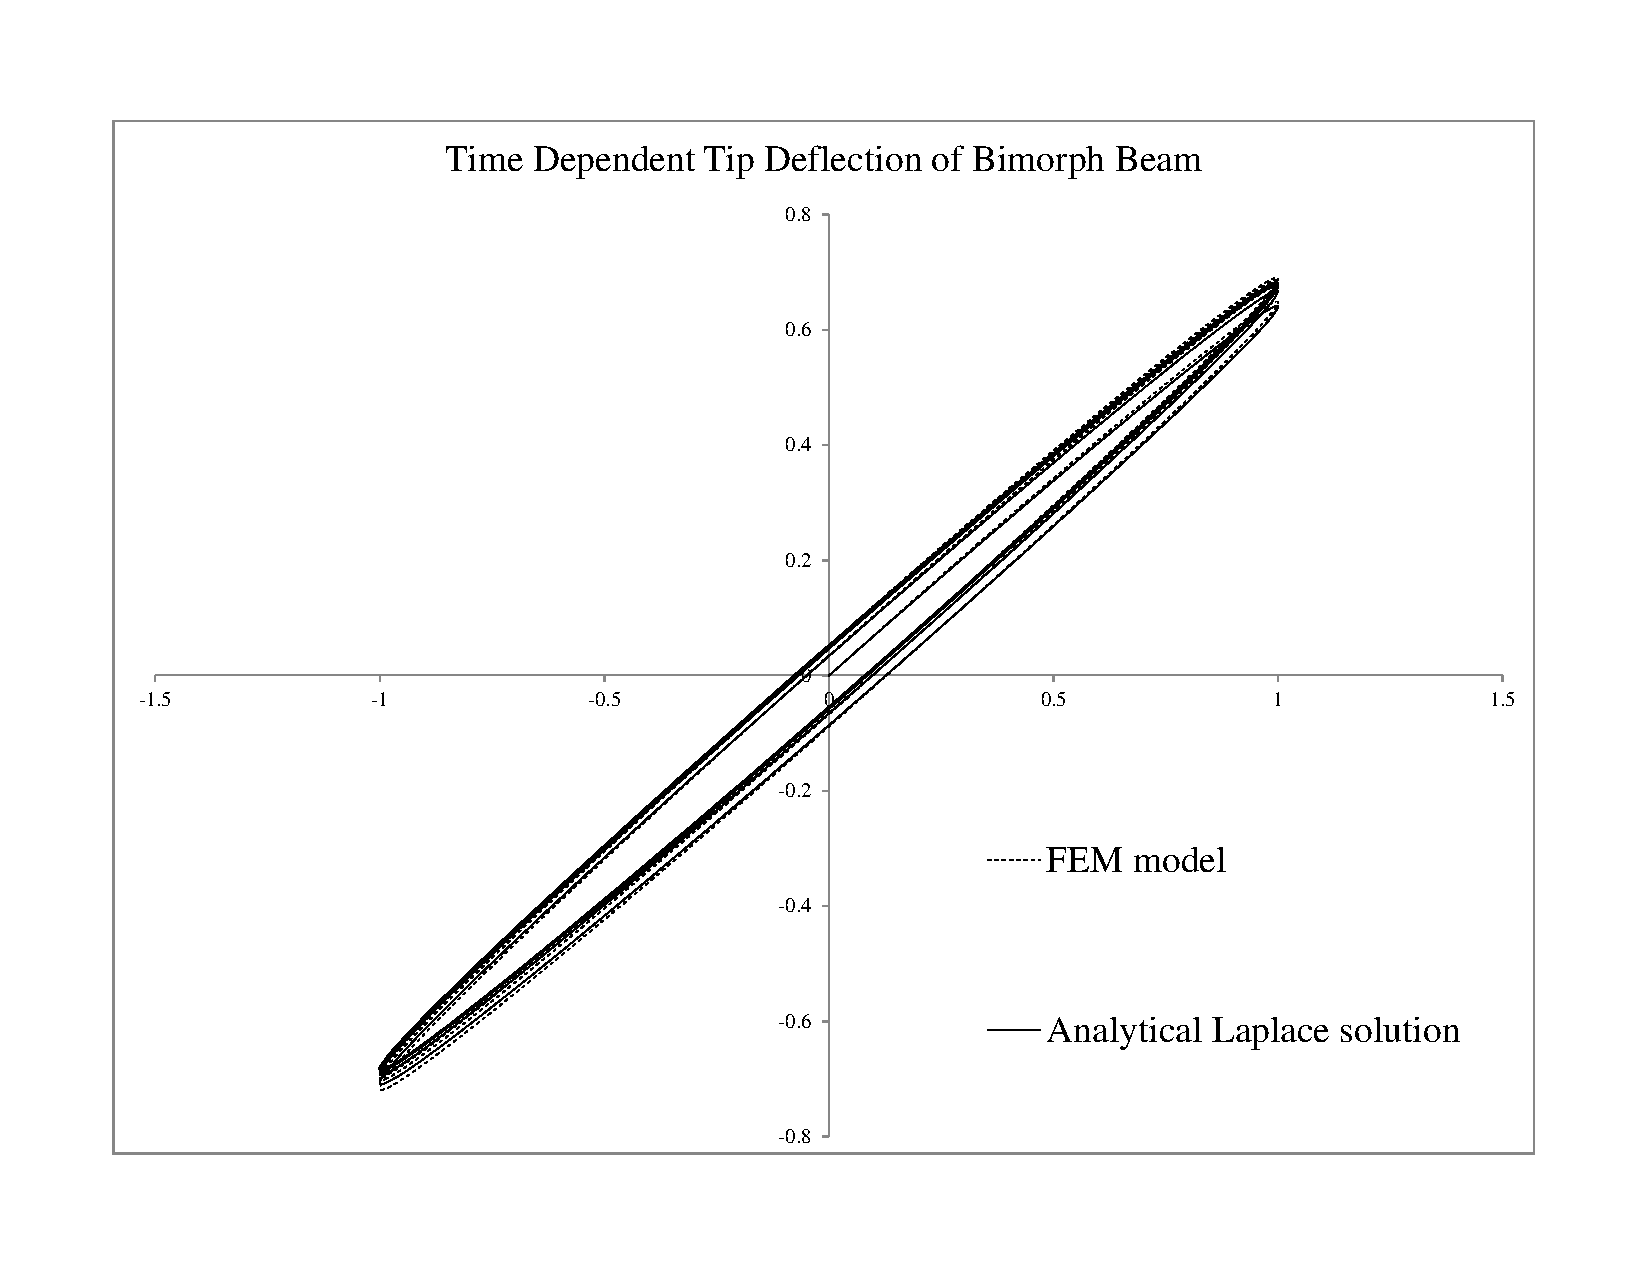
\includegraphics[width=6.0in]{./chap_4_structural_analyses/pdf_beam/result_tip_deflection_of_bimorph_beam.pdf}
\caption{Tip deflection of bimorph beam, comparing Laplace solution with numerical recursive method}
\label{fig:result_tip_deflection_of_bimorph_beam}
\end{figure}
Using these values in equations (\ref{eqn:history_dependent_stress_and_strain})-(\ref{eqn:inverse_laplace_of_transverse_displace_ment}) and taking inverse of the Laplace transform,
 the analytical solution for the time dependent deflection of the beam is:

\begin{equation}
\begin{aligned}
u_3(x_1,t)=\frac{A(t)}{B(t)}
\end{aligned}
\label{EQN:PVDF_beam_closed_form_solution}
\end{equation}
where $A(t)$ and $B(t)$ are the solutions of time dependent deformation that is obtained by a commercial computer algebra system, Maple.
For the present case study with the material properties for PVDF and the kernel function that is defined above, are forms for $A(t)$ and $B(t)$ are:

\begin{equation}
\begin{aligned}
&A(t)=A_0 e^{-\lambda_{A_0} t}+A_1 sin(2\pi \lambda_{A_1} t)+A_2 cos(2\pi
\lambda_{A_2} t)
\\
&B(t)=B_0 e^{-\lambda_{B_0} t}+B_1 sin(2\pi \lambda_{B_1} t)+B_2 cos(2\pi
\lambda_{B_2} t)
\end{aligned}
\label{EQN:PVDF_beam_closed_form_solution_functions}
\end{equation}
where the constants for this equation are presented in table \ref{table:PVDF_bimorph_time_dependent_solution_coefficients}.
The analytical solution is compared with the numerical solution from the recursive finite element analyses.
A 3D quadratic element with 20 nodes is used for finite element.
It is noted that quadratic elements shown to be more accurate in dealing with bending.
% The recursive integration in FE model technique is used to capture the time dependent effect.
The result from analytical solution and finite element analyses are compared in figure \ref{fig:result_tip_deflection_of_bimorph_beam}.
A good match between the Laplace transform method and numerical solution is observed.
This validates the recursive integration algorithm for the linear time-dependent electro-mechanical responses, which are implemented in finite elements.

\begin{table}
\caption{Coefficients for close form time dependent solution of PVDF beam}
\centering
\begin{tabular}{ccccc} \hline
n & $A_n$ & $B_n$ & $\lambda_{A_n}$& $\lambda_{B_n}$\\ \hline
0 & $-4.462664015\times 10^{19}$ & $8.333333335\times 10^{17}$ & -1.0 & 0.0\\ 
1 & $5.678974503\times 10^{20}$ & $1.326291193\times 10^9$ & 1.0 & 1.0\\ 
2 & $4.462664015\times 10^{19}$ & $0$ & 1.0 & 0.0 \\ \hline
\end{tabular}
\label{table:PVDF_bimorph_time_dependent_solution_coefficients}
\end{table}

The nonlinear electro-mechanical deflection of an active beam has been experimentally observed by Lin et al. \cite{Li2004959}.
This experiment is used to validate the nonlinear and time dependent closed form solution.
The beam has three layers, two piezoelectric and one metal substrate.
A metallic layer is placed in the middle of the beam with thickness of $h_s=0.0075in$. % or $h_s=127 \mu m$.
The substrate is made of stainless steel and its elastic modulus is taken to be $E_s=C_s=180 GPa$.
Two piezoelectric active layer are placed on the top and bottom of the substrate with thickness of $h_p=0.005in$. % or $h_p=190.5 \mu m$ each.
These layers are activated by electric potential.
The frequency of the excitation is 1Hz and the electric potential is applied with amplitude of 100 V.
The beam's length is $L=1.5 in$. % or $L=38.1 mm$.
The beam's width is $b=0.375 in$. % or $L=952.5 \mu m$.
The stiffness of piezoelectric layers in the longitudinal and transverse direction are reported as $E^L_p=C_p=63 GPa$ and $E^T_p=49 GPa$, respectively.
The electro-mechanical coupling stress is considered to be a nonlinear cubic function of electric field.

\begin{equation}
\sigma^e_{11}(E_3)= e^0_{311}E_3+e^2_{311}E^3_3
\label{EQN:cubic_coupling_stress_three_layer_beam}
\end{equation}
where the constants are taken to $e^0_{311}=14.5 C/m^2$ and $e^2_{311}=-6 pC/m^2$.
Moreover, the time dependent kernel function is taken as
\begin{equation}
K_e(t)=K^e_0+K^e_1exp(-\lambda_1 t )
\label{EQN:time_dependent_kernel}
\end{equation}
where the Prony constants are taken as: $K^e_0=1.7$, $K^e_1=-0.7$ and $\lambda_1=-0.7$.
The beam is constrained to be simply supported.
% They have designed an actuator with four simply supported beam.
% The actuator is designed with two beam at each side.
% Two beam are connected in serial in the way that their central deflection will add up.
The result from the deflection produced by the actuator along with the applied voltage is reported in \cite{Li2004959}.
This comparison is shown in figure \ref{fig:electric_volt_vs_displacement_three_layer_beam}.
The cubic approximation of the electro-mechanical coupling is close enough to the experimental data.
\\

\begin{figure}
\centering
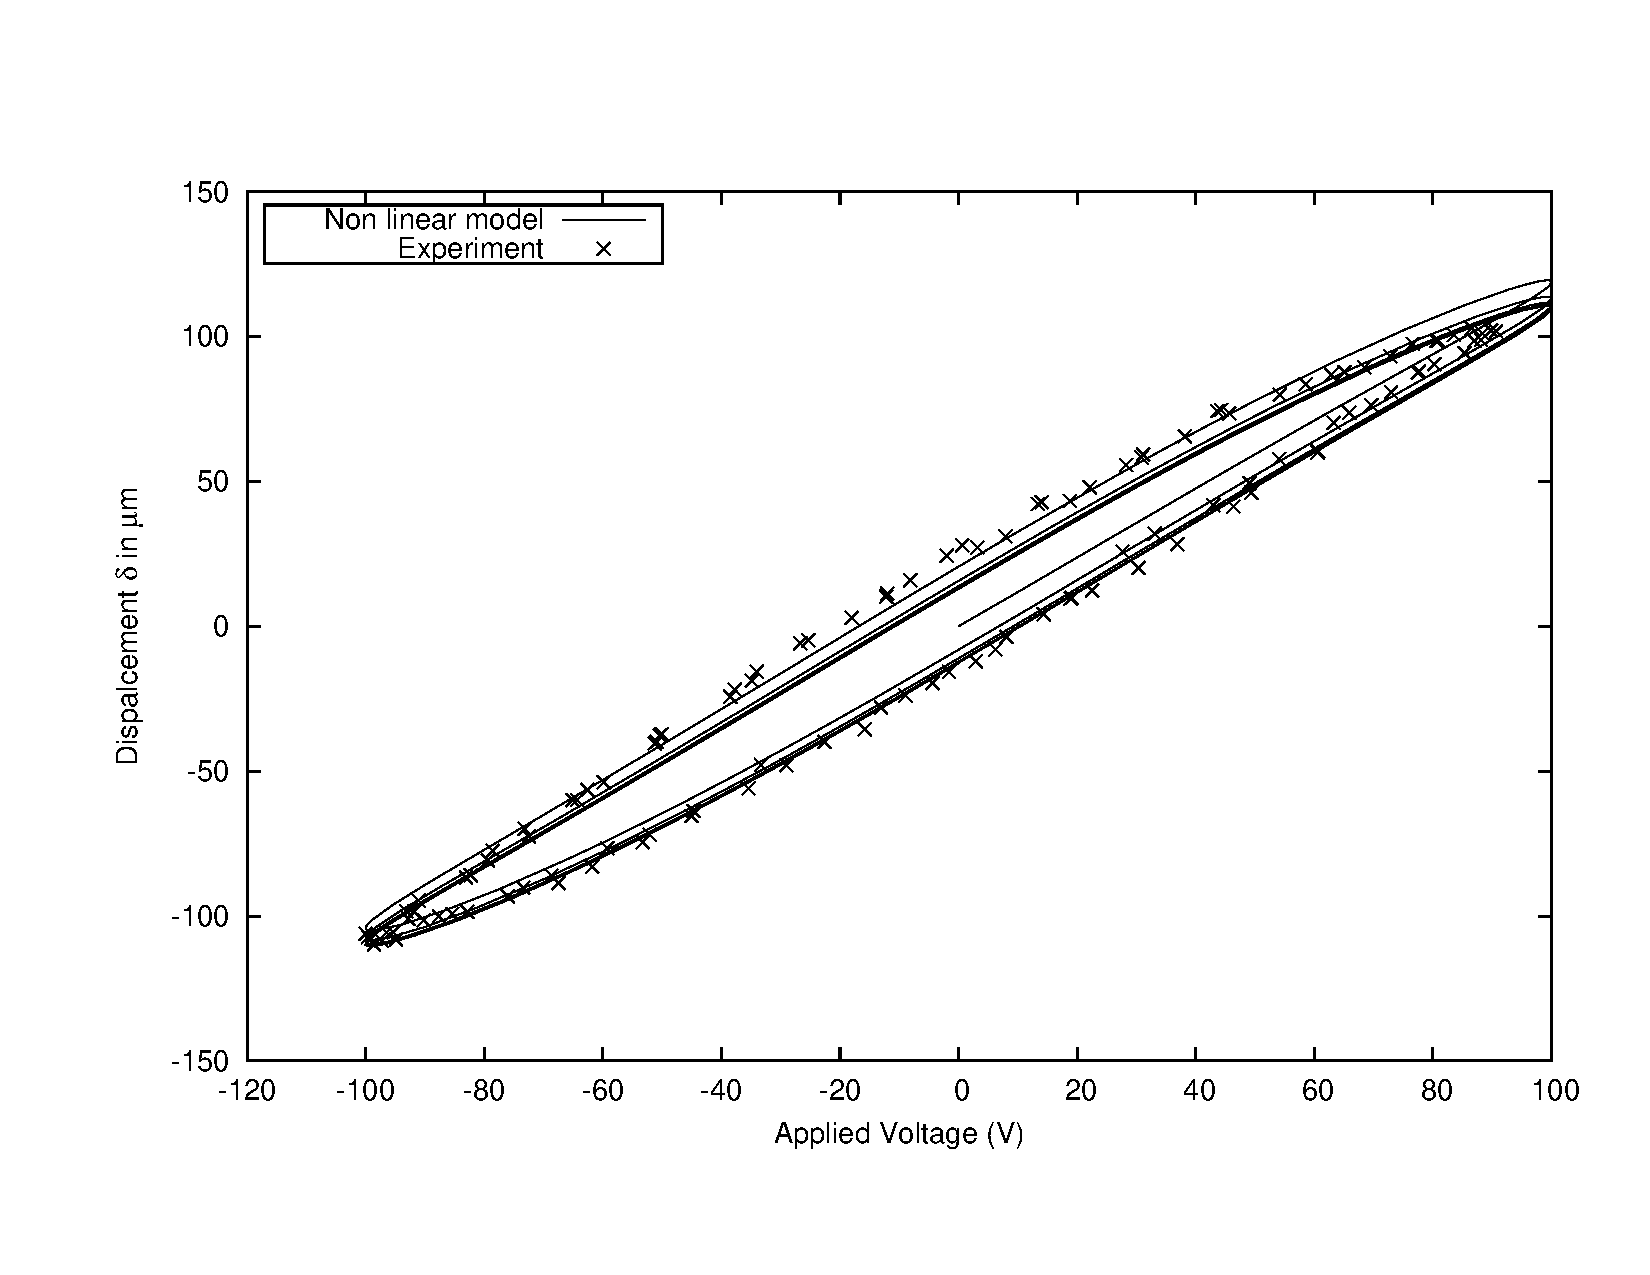
\includegraphics[width=6.0in]{./chap_4_structural_analyses/pdf_beam/electric_field_vs_displacement_three_layer_beam.pdf}
\caption{Experimental result \cite{Li2004959} compared with Laplace solution of an actuator made of three layer active beam}
\label{fig:electric_volt_vs_displacement_three_layer_beam}
\end{figure}

\subsection{Effect of Frequency on the Hysteresis Responses of Active Beams}
The effect of different histories of electric potential inputs is also analyzed.
Consider a bimorph beam consisting of two layers of polarized piezoelectric ceramics and an elastic layer, as shown in figure \ref{fig:PVDF_beam_geometry}. % TK .
In order to produce a bending deflection in the beam, the two piezoelectric layers should undergo opposite tensile and compressive strains.
The beam is fixed at one end and the other end is left free;
 the top and bottom surfaces are under a traction free condition.
 A potential is applied at the top and bottom surfaces of the beam and the corresponding displacement is monitored.

\begin{figure}
\centering
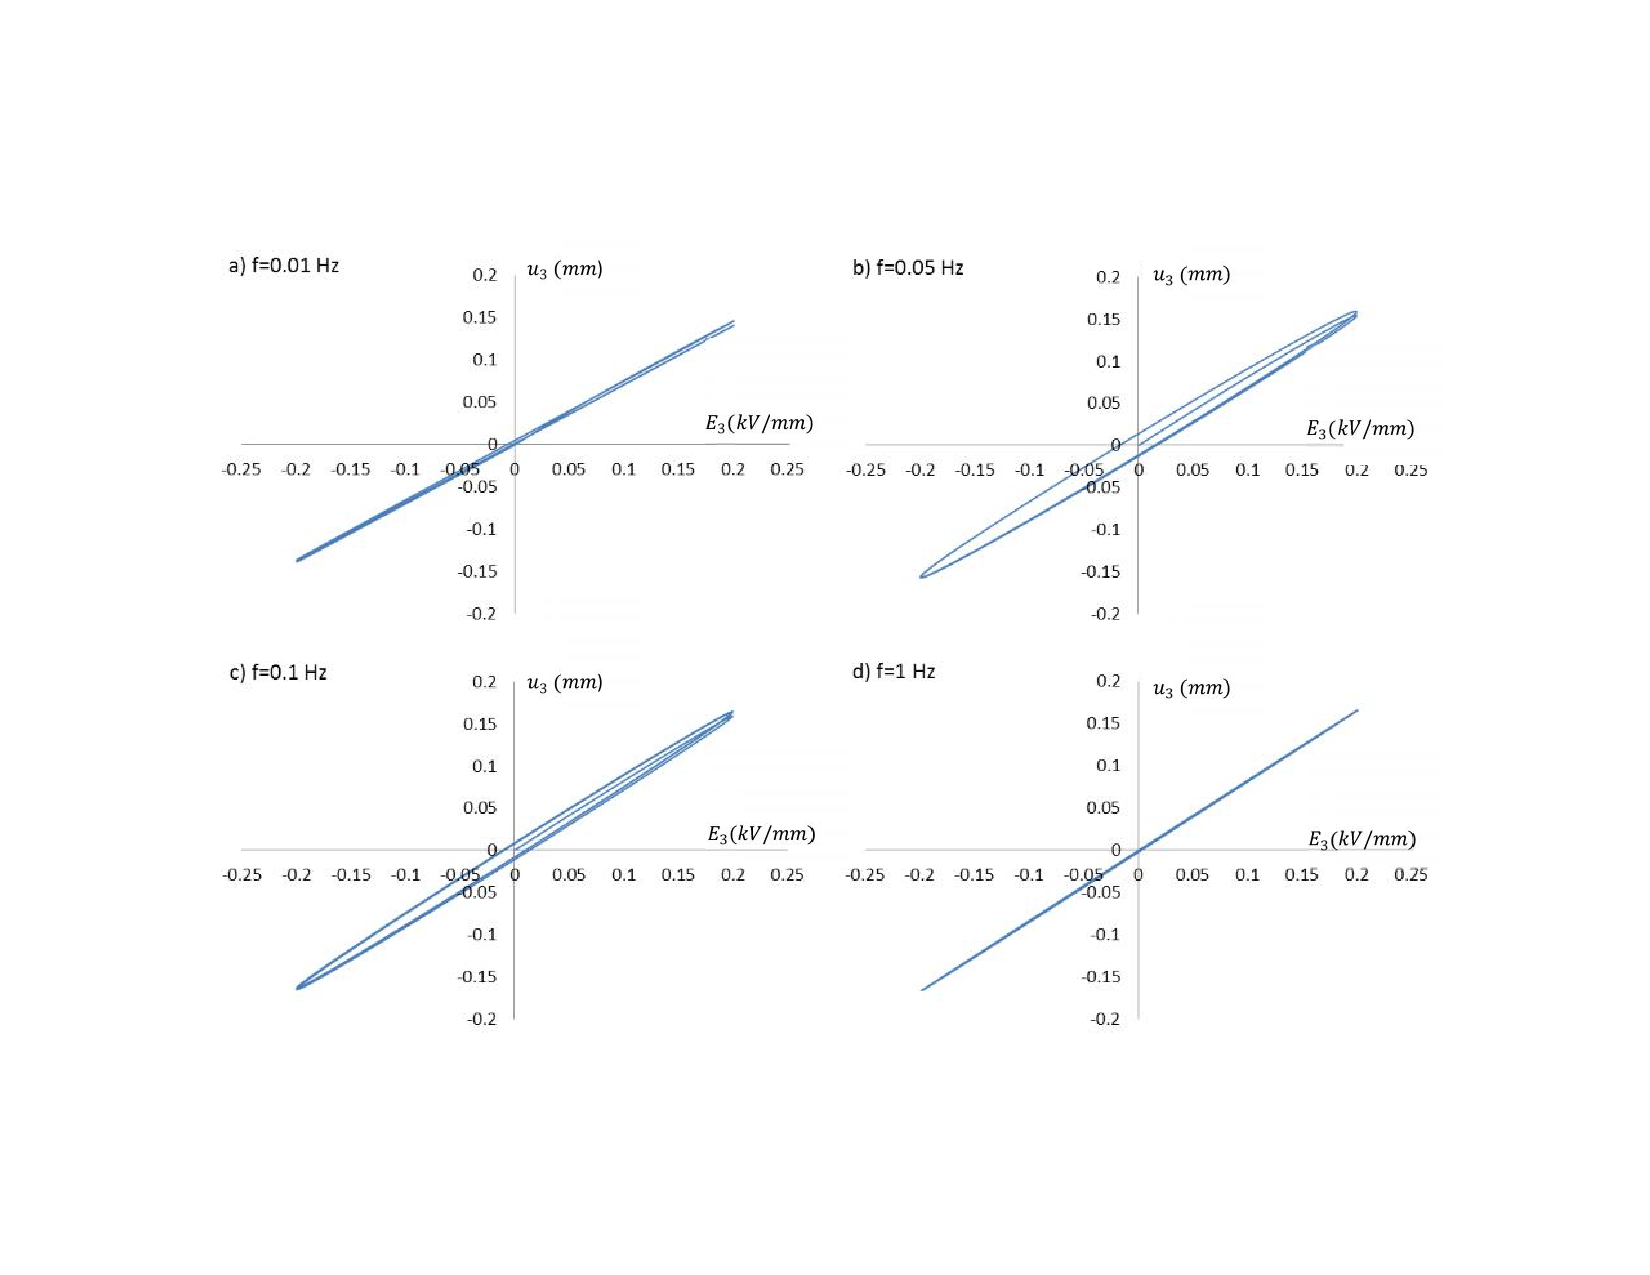
\includegraphics[width=6.0in]{./chap_4_structural_analyses/pdf_beam/result_tip_deflection_of_bimorph_beam_frequencies.pdf}
\caption{Tip deflection of bimorph beam, comparing observing effect of frequency of applied electric field}
\label{fig:result_tip_deflection_of_bimorph_beam_frequency}
\end{figure}

A bimorph beam without an elastic layer placed in between the piezoelectric layers is studied as it is shown in figure \ref{fig:bimorph_PVDF_beam_geometry}.
It is assumed that the beam is relatively slender so that it is sensible to adopt Euler-Bernoulli beam theory in finding the corresponding displacement of the bimorph beam.
Since a uniform voltage is prescribed on the top and bottom surfaces of the beam, the problem reduces to a pure bending problem.
The beam has a length of 100mm, width of 1mm and the thickness of each piezoelectric layer is 1mm.
The following time-dependent properties of PZT5A are used for the bending analyses.

\begin{equation}
\begin{aligned}
& C_p(t)=90 K^C(t) \, {GPa}      &K^C(t)=1+exp(-0.02 t)/3 \\
& e(t)=-5.35 K^e(t) \, C/m^2 &K^e(t)=1+exp(-0.2 t)/4
\label{Eqn:beam_frequency_material_properties}
\end{aligned}
\end{equation}

A sinusoidal input of an electric potential with various frequencies are applied.
figure \ref{fig:result_tip_deflection_of_bimorph_beam_frequency} illustrates hysteresis response of the bending of the bimorph beam.
The displacements are measured at the free end ($x_1$ =100mm).
When the rate of loading is comparable to the characteristics time,
the effect of time-dependent material properties on the hysteretic response becomes significant,
as shown by the response with frequencies of 0.05Hz and 0.1Hz.
When the rate of loading is relatively fast (or slow) with regards to the characteristics time, i.e. f=0.01Hz and 1Hz,
 insignificant (less pronounced) time-dependent effect is shown, indicated by narrow ellipsoidal shapes.
 
% \section{Large Deformation Analyses}
% In this section, large deformation analyses of slender beams is discussed.
% We use the bimorph beam geometry that was discussed in the previous example for large deformation analyses.
% The geometry of this beam is introduced in figure \ref{fig:bimorph_PVDF_beam_geometry}.
% In order to validate the result from finite element model, the closed form formulation for simple case of folding of a biomorph beam is considered.

% The Green St. Venant strain induced in the material due to deformations is a quadratic function of the displacement gradient \cite{Lai2009}.
% If the deformation is large then the nonlinear term of the strain cannot be disregarded.
% The quadratic function for the strain displacement relationship is defined as:

% \begin{equation}
% \varepsilon_{ij}=\frac{u_{i,j}+u_{j,i}}{2}+\sum_{m=1}^{3} \frac{u_{m,i}u_{m,j}}{2}
% \label{EQN:large_displacement_strain}
% \end{equation}

% Equation (\ref{EQN:large_displacement_strain}) is the more general form of infinitesimal strain theory that is represented in equation (\ref{EQN:Linear_Electric_Field}).
% The model is already developed based on nonlinear formulation for multi-functional material.
% Therefore, only the terms for strain should be modified in order to capture large deformation.

% It is possible to present analytical solutions for folding of beams \cite{Muliana2014}.
% The bimorph beam that is considered for large deformation is only under bending due to electric field.
% Therefore, the stretch in the beam is neglected.
% The strain is assumed linear in stress and the linear constitutive equations presented in equations (\ref{stress_1D_const_eqn_beam:EQN}) and (\ref{resultant_strain_beam:EQN}) are considered for the analyses. 
% The internal bending moment of the beam due to the mechanical strain can be presented as \cite{Muliana2014}:

% \begin{equation}
% M^m_{11}=E_{1} I_{11} \acute{\phi}
% \label{EQN:internal_bending_moment_beam}
% \end{equation}
% where 
% $E_{1}$ is the Young modulus and it is same as $C_p$,
% $I_{11}$ is the second moment of area that is $h_p^3/12$ in the case of bimorph geometry shown in figure \ref{fig:bimorph_PVDF_beam_geometry},
% $\acute{\phi}$ is the curvature of the beam can be presented as $\acute{\phi}=1/r$ where $r$ is the radius of folded shape of beam.      
% In case of a complete folding of the beam, the radius of curvature for beam will be $r=\frac{L}{2\pi}$, where $L$ is the length of beam.

% The electrical bending moment of beam due to electric field using equations \ref{stress_1D_const_eqn_beam:EQN} and \ref{resultant_strain_beam:EQN} can be presented as:
% \begin{equation}
% M^e_{11}=\frac{e_p  h_p  V}{2}
% \label{EQN:electric_bending_moment_beam}
% \end{equation}
% There is no other external force or moment is acting on the beam. 
% Then, the equilibrium equation in the beam can be satisfied at each point on the neutral axis, thus $M^m_{11}=M^e_{11}$.
 
% Considering the mechanical and electrical properties for the PVDF beam the electric potential needed to completely fold the PVDF bimorph beam will be 
% \begin{equation}
% V_{fold}=\frac{h_p^2 \pi C_p}{3 e_p L}
% \label{EQN:electric_potential_to_fold}
% \end{equation}
% Using the electro-mechanical material properties and geometries of bimorph beam that were discussed before the electric potential for folding the beam is $V_{fold}=455kV$.
% This electric potential is applied to the central electrode of the biomorph beam in the finite element analyses.
% The result from this analyses is shown in figure \ref{fig:pvdf_beam_folding}.
% It can be seen that a complete folding is captured by taking the nonlinear kinematics into account as it is expected from the analytical solution presented.
% % This validates the nonlinear geometric analyses of developed multi-functional finite element model.
% % It is noted for the sake of consistency with the other simulation reported in the literature only the transverse electro-mechanical coupling is considered in this simulation.
% % In the real situation the complete folding of bimorph beam will happen with much lower electric potential due to normal electro-mechanical coupling and incompressibility of polymer that are disregarded in this analyses. 
% \\  
 
% \begin{figure}
% \centering
% 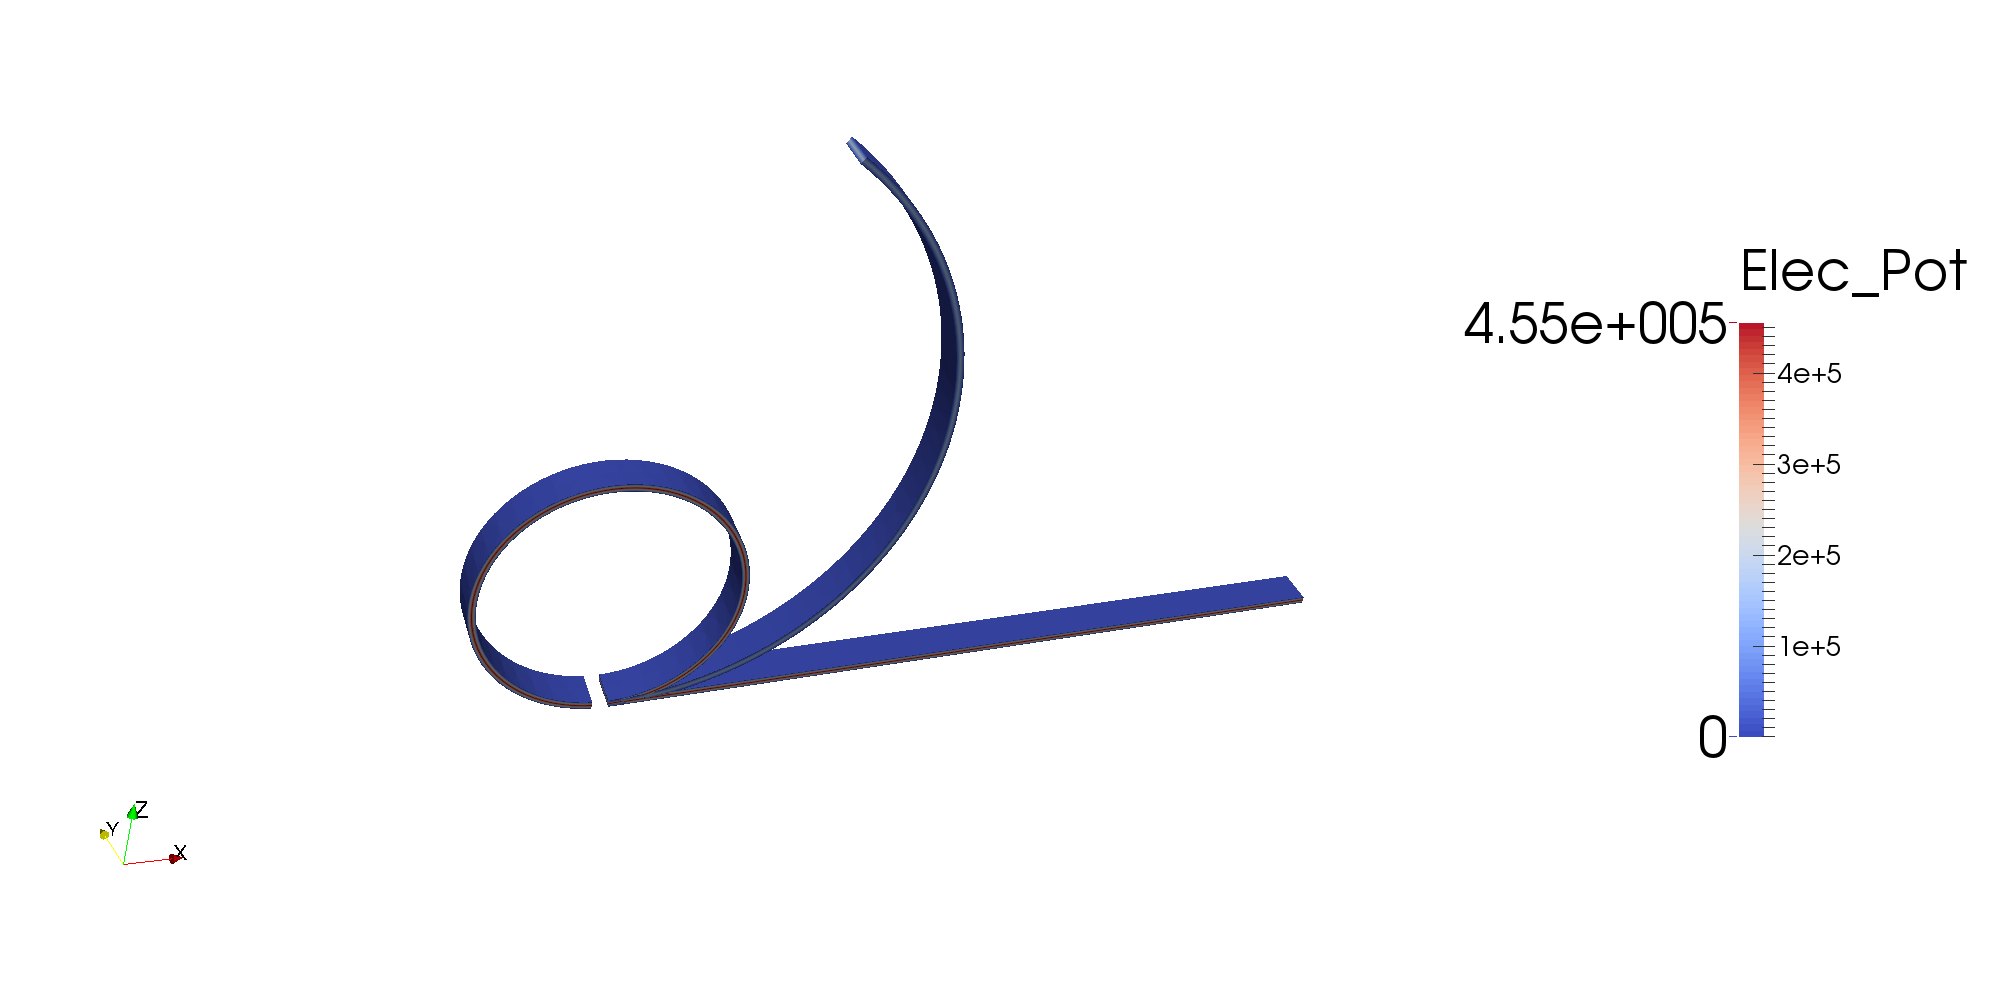
\includegraphics[trim = 00mm 0mm 00mm 0mm,clip=true,width=7.0in]{./chap_4_structural_analyses/pvdf_folding_beam/folding_pvdf_beam.png}
% \caption{Folding of bimorph PVDF beam under very high electric potential}
% \label{fig:pvdf_beam_folding} 
% \end{figure}
\section{Active Fiber Composites}
Active Fiber Composite (AFC) is an active material that is designed to amplify the deflection due to piezo-electric effect. In AFCs PZT5A fibers are embedded in the epoxy matrix and are aligned along the longitudinal direction. The electric field is applied to PZT5A fiber through the aluminum electrode fingers that are placed on the top and bottom of the fibers. Aluminum electrode fingers are aligned perpendicular to the longitudinal axis of fiber in the width direction of AFCs. Electrodes that are placed on the top and bottom surfaces of the AFC have the same electric potential. Therefore, the electric field on the central plane of the AFC is zero. Electrodes that are adjacent to each other in the longitudinal direction of the AFC have the opposite electric potentials. As a result, an electric field is formed along the longitudinal direction of fibers and the electric field is not uniformly distributed along the fibers. The electric field in the gap between electrodes is directly proportional to the value of applied potential and inversely proportional to the distance between electrodes. An example of AFCs is shown in figure \ref{fig:afc_picture_from_lap}.
A schematic of the placement of fibers and electrodes is shown in figure \ref{fig:schematic_afc_unit_cell} \cite{jemai2014mathematical}.

\begin{figure} 
\centering
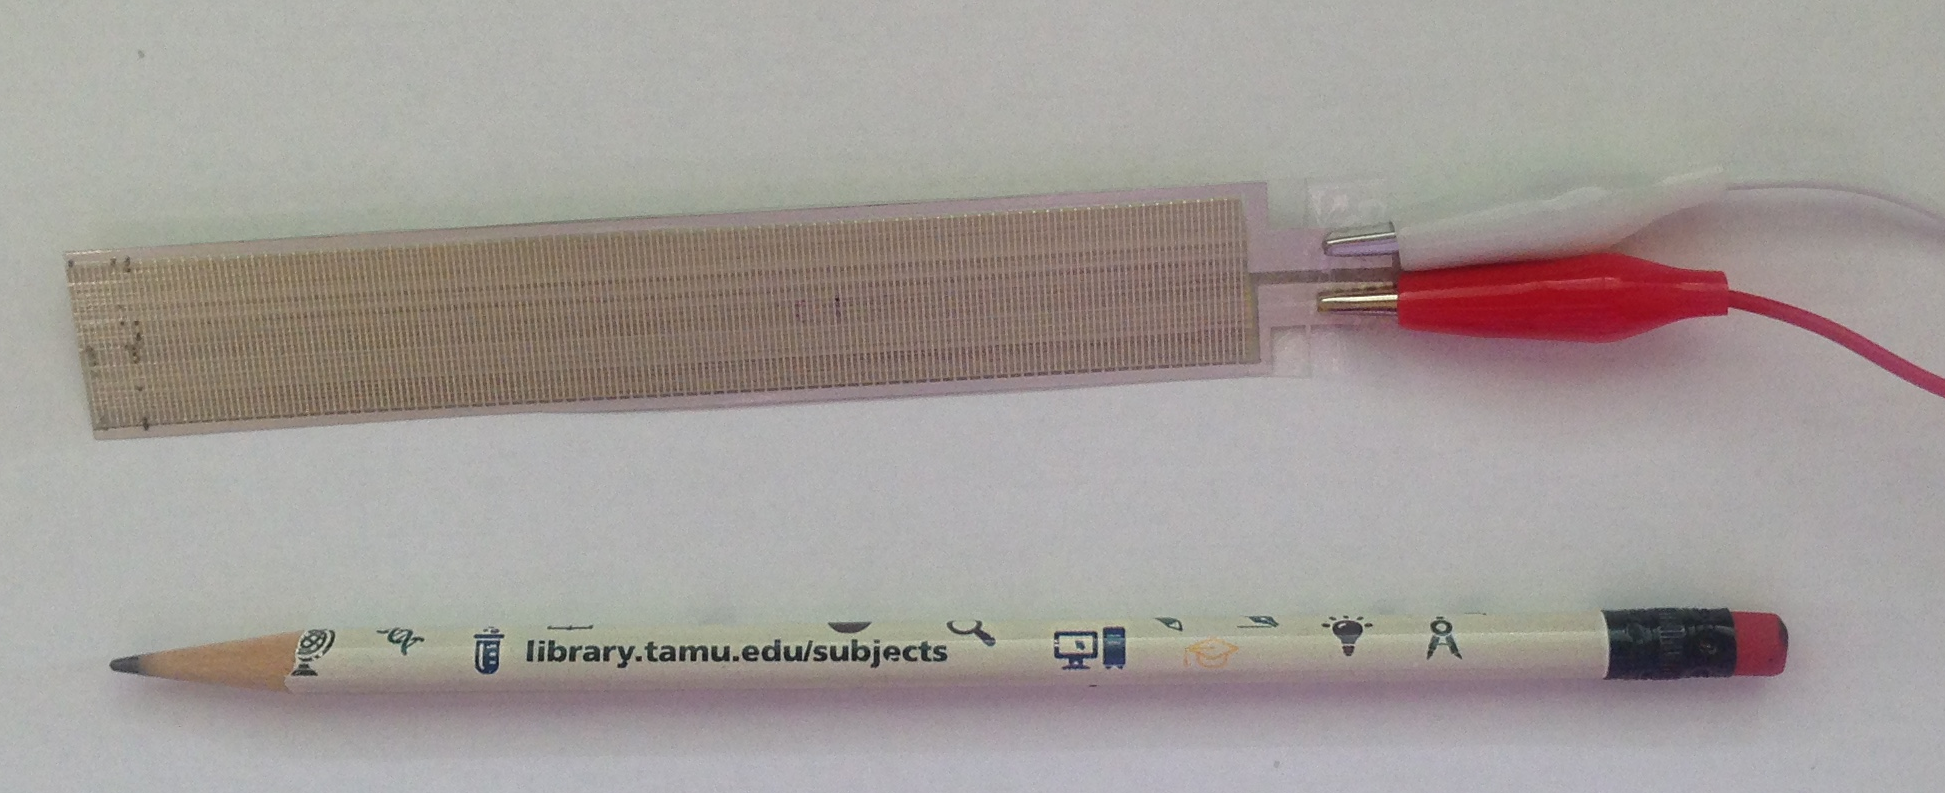
\includegraphics[width=6.0in]{./chap_4_structural_analyses/afc_unit_cell/afc_picture_from_lap.png}
\caption{Active fiber composite and applying electric potential}
\label{fig:afc_picture_from_lap}
\end{figure}
The configuration of AFC patch is symmetric with respect to its thickness direction.
Moreover, there is a periodic pattern in the placement of fibers, electrodes and matrix in the longitudinal direction of AFC.
Due to this symmetry and periodic configuration, a unit cell model for AFC is defined as a representative microstructure.
This unit cell is used to determine the overall electro-mechanical behavior of AFC.  

\subsection{Unit Cell of an Active Fiber Composite}
The smallest possible unit cell of AFC is considered in order to determine its overall behavior.
This unit cell contains one quarter of fiber in the space between two electrodes as shown in figure \ref{fig:geometry_unit_cell_afc}.
The unit cell has dimensions of $L_1 \times L_2 \times L_3 =140 \mu m \times 175 \mu m \times 750 \mu m$.
A PZT5A fiber with the radius of $125 \mu m$ is embedded in epoxy matrix as shown in figure \ref{fig:geometry_unit_cell_afc} (right).
Two aluminum electrodes are seen in the unit cell under the fiber with thickness of $10 \mu m$. 
Each aluminum electrode finger is $250 \mu m$ long and due to periodicity of the microstructure only half of each electrode is considered in the unit cell.
There is $500 \mu m$ gap between two electrodes that is filled with epoxy.
Moreover, there is $4 \mu m$ vertical threshold between the electrodes and PZT5A fiber that is filled with epoxy.
The electric potential applied to the aluminum electrodes induces electric field inside the epoxy and also inside the PZT5A fiber.
\begin{figure} 
\centering
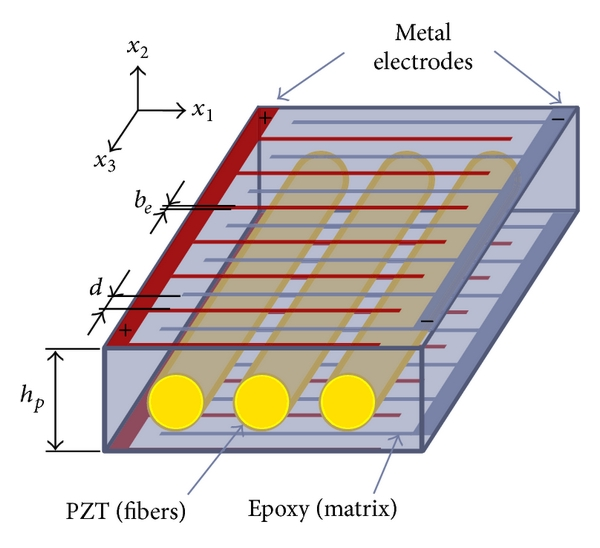
\includegraphics[width=3.0in]{./chap_4_structural_analyses/afc_unit_cell/schematic_afc_unit_cell.jpg}
\caption{Schematic for placement of fibers and electrodes in the epoxy matrix \cite{jemai2014mathematical}}
\label{fig:schematic_afc_unit_cell}
\end{figure}
% \blfootnote{*Reprinted with permission from "Mathematical modeling of an active-fiber composite energy harvester with interdigitated electrodes" by Jemai, A., Najar, F., Chafra, M., Ounaies, Z., (2014). \textit{Shock and Vibration}, 94, 1-9,  Copyright 2014 Hindawi Publishing Corporation}
\begin{figure}
\centering
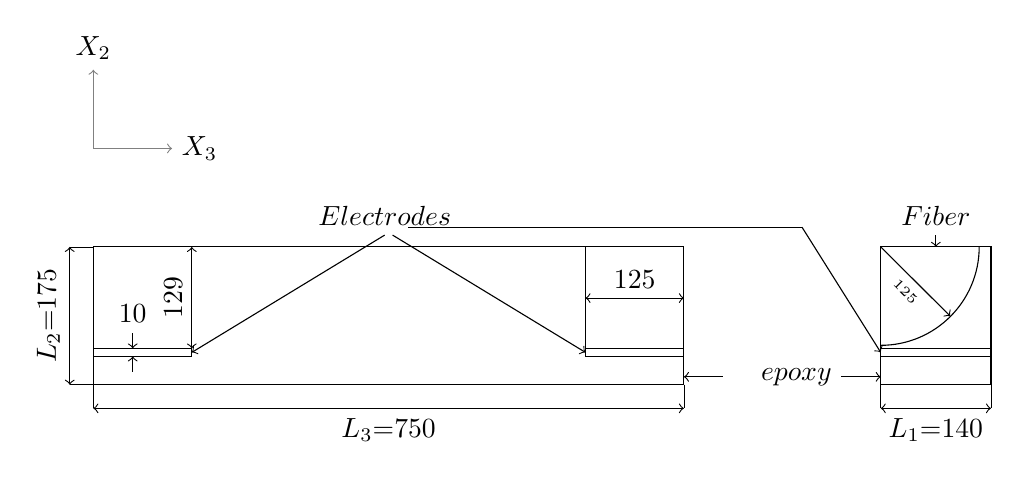
\begin{tikzpicture}  

\draw (0,0) rectangle (7.50,1.75) ; 

\draw (0,0.36) rectangle (1.25,0.46);
\draw (6.25,0.36) rectangle (7.50,0.46); 

 
% dimension in the middle from top to electrode 
\draw [<->] (1.25,0.46) -- (1.25,1.75) node [sloped,midway,above] {129};

% right dimension for  right electrode
\draw  [<-] (0.5,0.46)--(0.5,0.66) node [above] {10};
\draw  [<-] (0.5,0.36)--(0.5,0.16);

%vertical dimenstion
\draw [<->] (-0.30,0) --  (-0.30,1.75) node [sloped,midway,above] {$L_2$=175};
\draw [very thin,-] (0.0,0) --  (-0.30,0);
\draw [very thin,-] (0.0,1.75) --  (-0.30,1.75);

% horizental dimension of electrode
\draw [very thin,-] (6.25,0.36) -- (6.25,1.75);
\draw [<->] (6.25,1.1) --  (7.5,1.1)  node [sloped,midway,above] {125};

%horizentoal dimenstion
\draw [<->] (0,-0.30) --  (7.50,-0.30) node [sloped,midway,below] {$L_3$=750};
\draw [very thin,-] (0,0) --  (0,-0.30);
\draw [very thin,-] (7.5,0) --  (7.5,-0.30);

%% The left view
\draw (10.0,0) rectangle (11.4,1.75) ; 
%% The horizental dimension
\draw [<->] (10.0,-0.3)--  (11.4,-0.3) node [sloped,midway,below] {$L_1$=140};
\draw [very thin,-] (10.0,0) --  (10.0,-0.3);
\draw [very thin,-] (11.4,0) --  (11.4,-0.3);

%% The fiber
\draw (11.25,1.75) arc  (0:-90:1.25) ; 
%% The electode in the view
\draw (10.0,0.36) rectangle (11.4,0.46) ;

%% The arrows for electrodes
\draw [<-] (1.25,0.41) -- (3.7,1.9) node [above] {$Electrodes$};
\draw [<-] (6.25,0.41) -- (3.8,1.9) ;
\draw [<-] (10.0,0.41) -- (9,2.0) ;
\draw (9,2.0) -- (4.00,2.0) ;

%% The arrows for fiber
\draw [<-] (10.7,1.75) -- (10.7,1.9) node [above] {$Fiber$};

%% The arrows for epoxy
\draw [<-] (10.0,0.10) -- (9.5,0.1) node [left] {$epoxy$};
\draw [<-] (7.50,0.10) -- (8.0,0.1);

%% The radial dimension
\draw [<-] (10.883,0.8698) -- (10.0,1.75)  node [sloped,midway,below]{\tiny 125};


\draw[latex-latex, thin, draw=gray] [->](0,3)--(1,3) node [right] {$X_3$}; %
\draw[latex-latex, thin, draw=gray] [->](0,3)--(0,4) node [above] {$X_2$}; % 
 
\end{tikzpicture}
\caption{Geometry of AFC unit cell (dimensions are in $\mu m$)}
\label{fig:geometry_unit_cell_afc}
\end{figure}

The mechanical response of epoxy is considered to be linear viscoelastic.
The epoxy has very small electro-mechanical coupling that can be neglected in the analyses.
The electric potential is transferred from the electrodes to fibers through the epoxy.
Therefore, the dielectric properties of epoxy have a significant effect on the overall electro-mechanical properties of AFC \cite{atitallah2014parametric}. 
The electric potential is applied to the two aluminum electrodes, which are shown in the unit cell in figure \ref{fig:geometry_unit_cell_afc}.
The embedded aluminum electrodes have $10 \mu m$ thickness.
It is noted that only half of each electrode is considered in this unit cell.
The length of each electrode is $250 \mu m$.
Two electrodes that are considered in the unit cell are charged with electric potentials with opposite signs.
The response of aluminum fingers embedded in the AFC is assumed linear elastic.

The periodic and symmetric boundary conditions are prescribed to the unit cell in order to model the effective behavior of AFC. 
The boundary conditions prescribed on the unit cell of AFC are given as follows:

\begin{equation}
\begin{aligned} 
& x_1=-\frac{L_1}{2}  ,& u_1=0 &\, , \frac{\partial \phi}{\partial x_1}=0        &\, ; \ x_1= \frac{L_1}{2}  ,& u_1=\bar{u_1} &\, ,  \frac{\partial \phi}{\partial x_1}=0   \\ 
& x_2=-\frac{L_2}{2}  ,& u_2=0 &\, , \frac{\partial \phi}{\partial x_2}=0        &\, ; \ x_2= \frac{L_2}{2}  ,& u_2=\bar{u_2} &\, ,  \frac{\partial \phi}{\partial x_2}=0   \\ 
& x_2=-\frac{L_3}{2}  ,& u_2=0 &\, , \frac{\partial \phi}{\partial x_3}=0        &\, ; \ x_3= \frac{L_3}{2}  ,& u_3=\bar{u_3} &\, , \frac{\partial \phi}{\partial x_3}=0    \\
\end{aligned}
\end{equation}
where the geometry of the unit cell shown in figure \ref{fig:geometry_unit_cell_afc} is defined in $x_1 \in [-L_1/2,L_1/2], x_2 \in [-L_2/2,L_2/2], x_3 \in [-L_3/2,L_3/2]$.
 

The matrix, electrodes and fibers are bonded together with adhesive. 
It is assumed that the adhesive has the same mechanical and electrical properties as the epoxy.
Only the piezoelectric fiber experiences electro-mechanical coupling due to the applied electric field.
The strain induced inside the fiber causes deformations of the unit cell.
The viscoelastic properties of the epoxy and the time
 dependent electro-mechanical response of piezo electric fiber can affect the overall deflection of the unit cell.
The finite element analyses for the nonlinear time-dependent electro-mechanical response are used to simulate and predict the behavior of AFC. 

The electric potential is applied to the electrodes in the unit cell.
The material properties that are considered for PZT5A fiber, epoxy matrix and aluminum electrodes are presented in table \ref{table:materila_properties_afc}.
The distribution of electric potential is shown in figure \ref{fig:electrip_potential_afc_pictur}.
In this picture the positive and negative electric potentials applied to the unit cell are shown.

\begin{table}
\caption{Material properties of AFC}
\centering
\begin{tabular}{ccccc} \hline
               & PZT5A & epoxy & Aluminum & \\ \hline 
Young's Modulus&60.06 & 1.5     & 69       &$GPa$    \\ 
Poisson's Ratio&$0.3$ & 0.35    & 0.33 &\\  
$e_{113}$      &-59.5 &         &      &$C/m^2$\\ 
$e_{311}$      &8.00&         &      &$C/m^2$\\ 
$e_{333}$      &-27.196  &         &      &$C/m^2$\\ 
$\kappa_{11}=\kappa_{22}$ &  $ 4  $ & $8.854  $ & &  pF/m \\ 
$\kappa_{33}$ & $2  $              & $8.854  $ & &  pF/m \\ 
${}^{0}K_{ijk}^{e}$&1.0& & &  \\ 
${}^{1}K_{ijk}^{e}$&-0.45& & & \\ 
${}^{0}\lambda_{ijk}^{e}$&0& & & s \\ 
${}^{1}\lambda_{ijk}^{e}$&1.5& & & s \\  
${}^{0}K_{ijkl}^{c}$& &1.0 & &  \\  
${}^{1}K_{ijkl}^{c}$& &0.4 & & \\ 
${}^{0}\lambda_{ijkl}^{c}$& &0&  & s\\ 
${}^{1}\lambda_{ijkl}^{c}$& &0.8 & & s \\ \hline 
\end{tabular}
\label{table:materila_properties_afc} 
\end{table}

\begin{figure} 
\centering
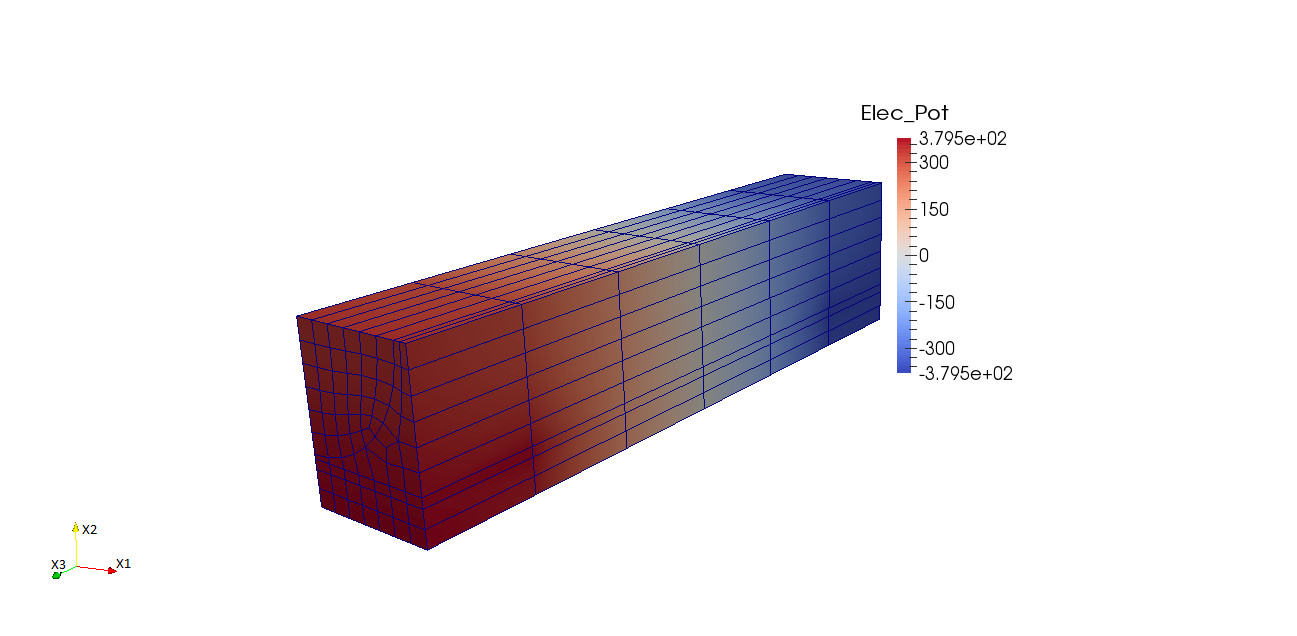
\includegraphics[width=5.0in]{./chap_4_structural_analyses/afc_unit_cell/afc_electrip_potential_distribution.png}
\caption{Distribution of electric potential in its unit cell of AFC (Electrode Voltage is 380V)}
\label{fig:electrip_potential_afc_pictur}  
\end{figure}  


\begin{figure} 
\centering
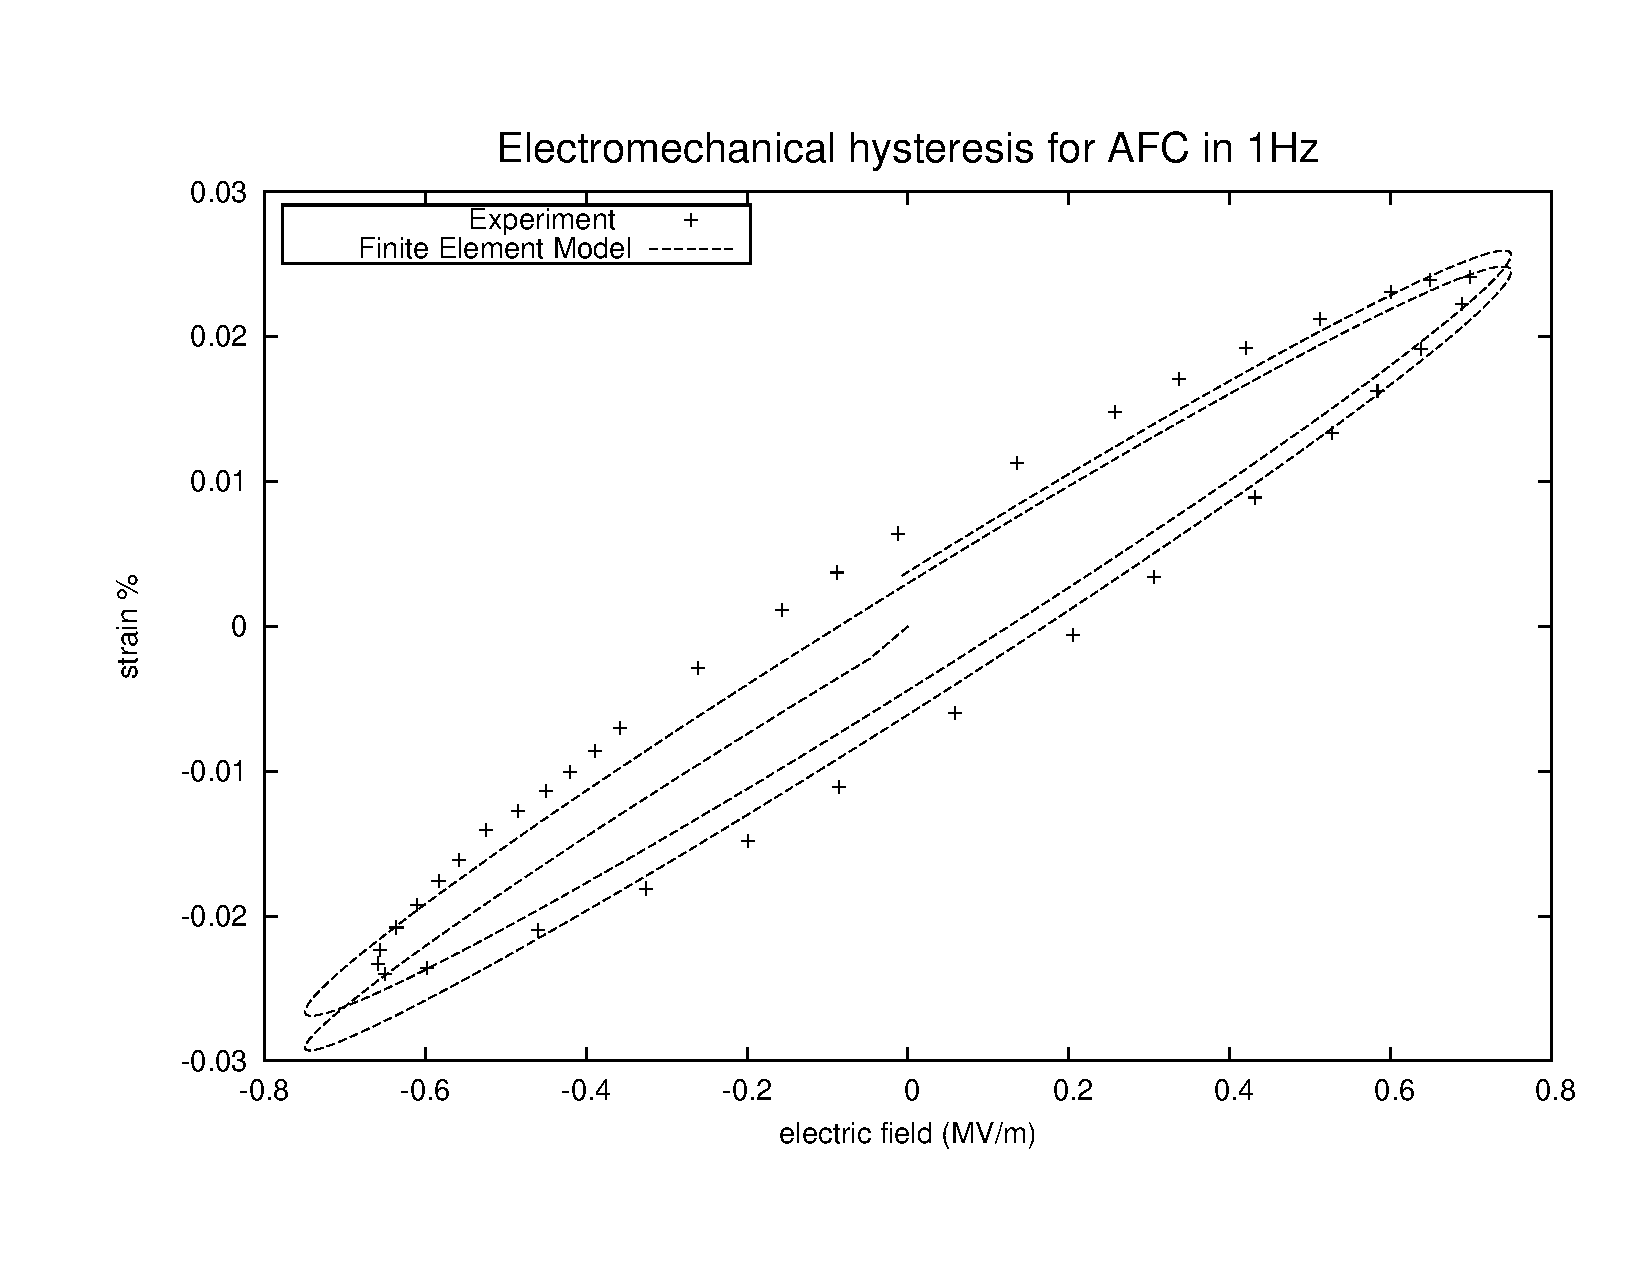
\includegraphics[width=5.0in]{./chap_4_structural_analyses/afc_unit_cell/comparison/afc_result_electric_field_vs_strain.pdf}
\caption{Electro-mechanical hysteresis at 1Hz compared with experiment}
\label{fig:afc_result_electric_field_vs_strain}
\end{figure} 

\subsection{Validating The AFC Model with Experiment Data}
Finite element analyses for AFC unit cell are validated with the existing experimental results.
The detailed experimental procedure is discussed in \cite{atillah2014}.
In order to calibrate the properties of PZT, line between two peaks of the hysteresis curve from experimental data is used to find the linear and time independent material properties.
The material properties for the epoxy and aluminum are taken from \cite{atitallah2014parametric}.
Aluminum is considered elastic.
Then, the width of hysteresis curve is used to determine the time-dependent coefficient presented in table \ref{table:materila_properties_afc}.
 
The comparison between experimental data and the results from FE analyses with linear time dependent electro-mechanical coupling for PZT is shown in figure \ref{fig:afc_result_electric_field_vs_strain}.
The hysteresis response shown in the deflection of this unit cell is due to the time dependent response of the epoxy matrix and also time dependent electro-mechanical coupling of piezo-electric fiber. 
There is good comparison between the experiments and FE analyses.
The distribution of displacement field in the unit cell is shown in figure \ref{afc_displacement_all:fig}.
As expected the value of displacement in the longitudinal ($X_3$-axis) direction is significantly larger than the other two directions.

\begin{figure}
\centering
\subcaptionbox{Displacement in $x_1$ (x) direction}
{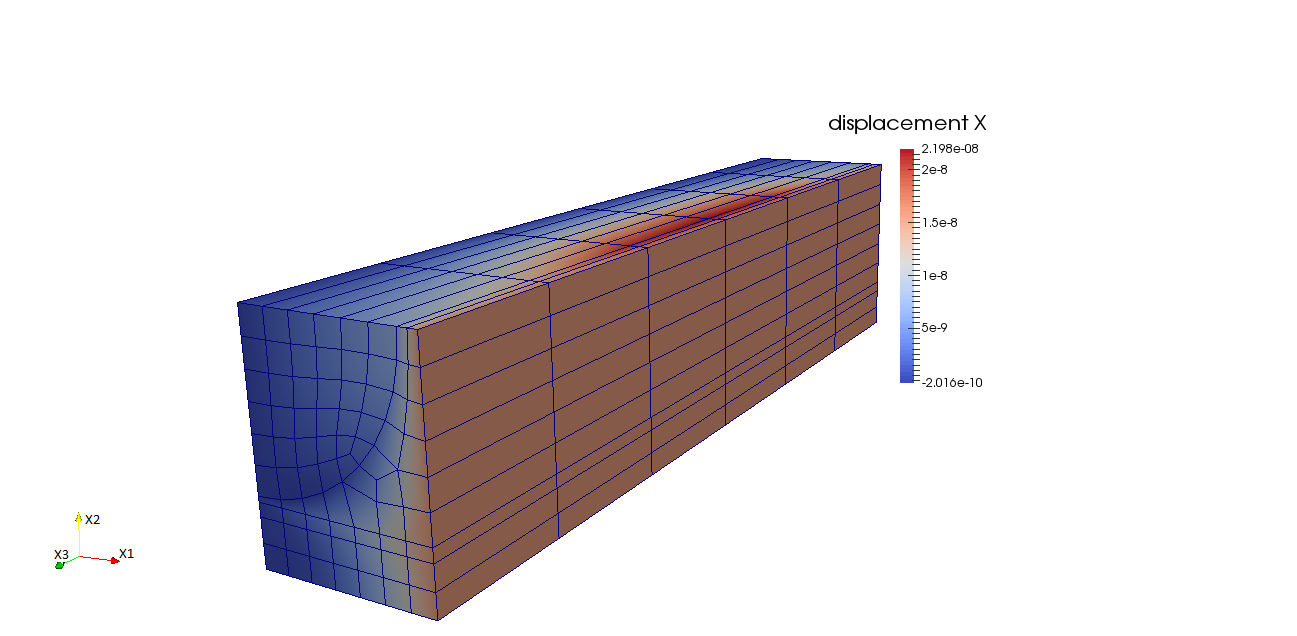
\includegraphics[width=4in]{./chap_4_structural_analyses/afc_unit_cell/afc_displacement_x.png}}
\subcaptionbox{Displacement in $x_2$ (y) direction}
{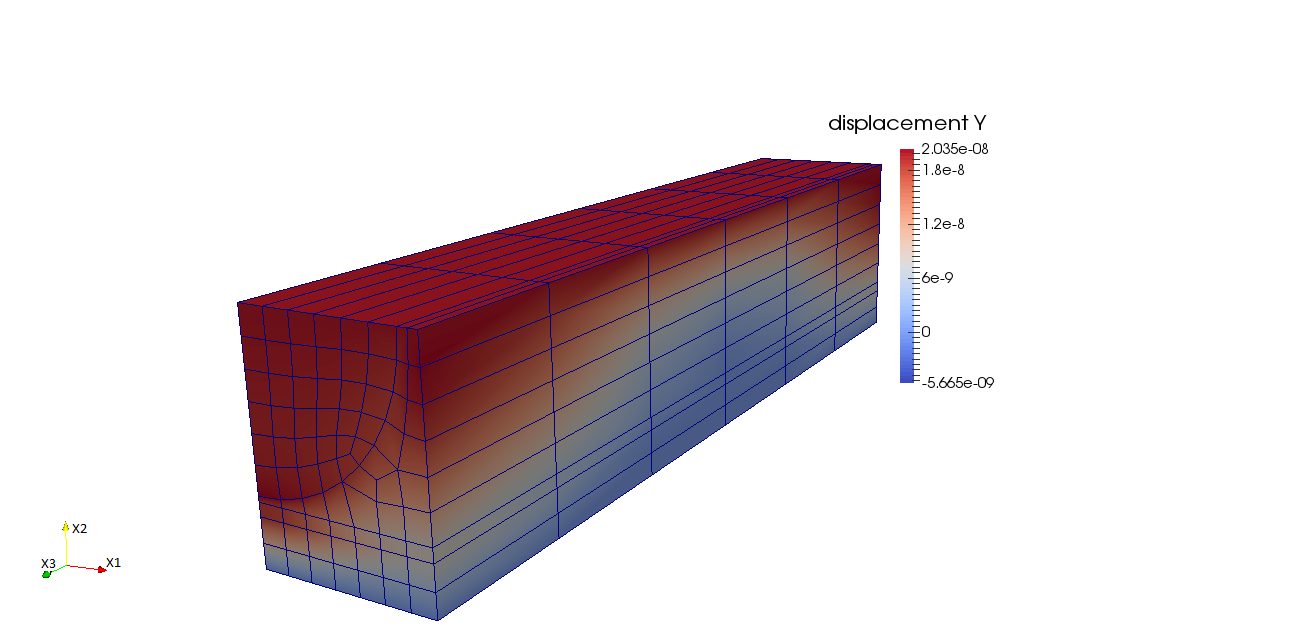
\includegraphics[width=4in]{./chap_4_structural_analyses/afc_unit_cell/afc_displacement_y.png}}
\subcaptionbox{Displacement in $x_3$ (z) direction}
{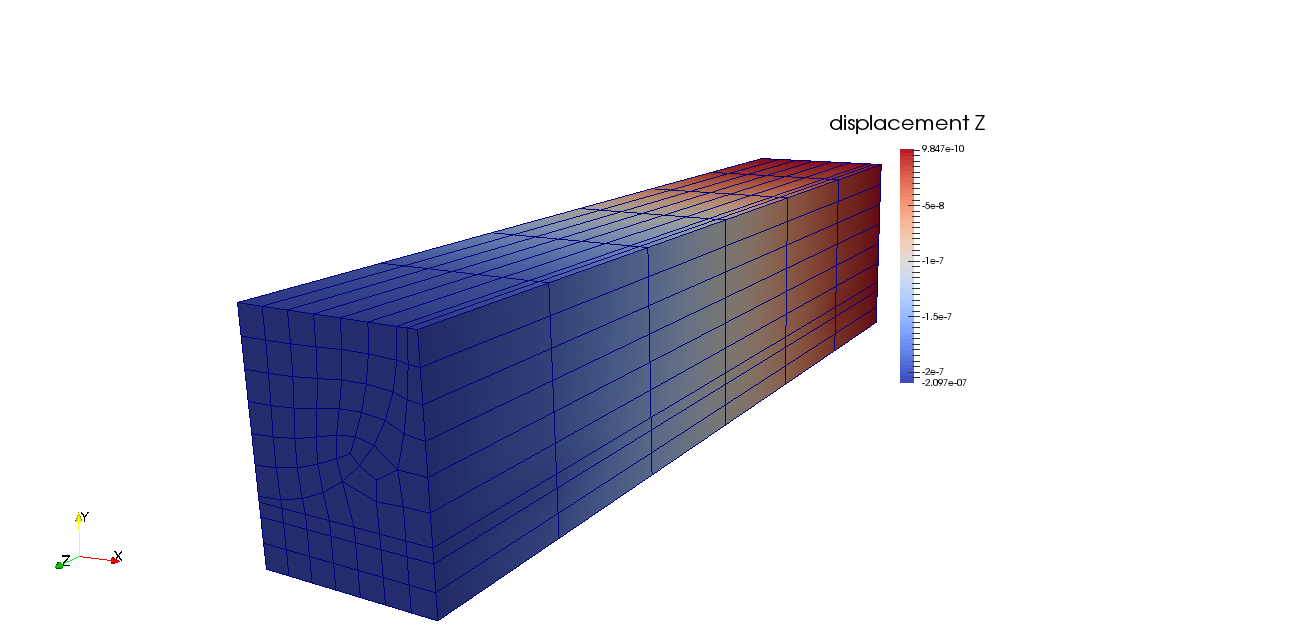
\includegraphics[width=4in]{./chap_4_structural_analyses/afc_unit_cell/afc_displacement_z.png}}
\caption{Displacement field distribution in unite cell of AFC in mm (Electrode Voltage is 380V)}
\label{afc_displacement_all:fig}
\end{figure}

At higher amplitudes of electric field, AFC shows nonlinear and time dependent response due to nonlinear electromechanical coupling. 
This effect is simulated using the QLV model that has been discussed in the previous chapters. 
A polynomial for the nonlinear electric field is considered. 
The material parameters for this model are presented in table \ref{table:non_linear_materila_properties_afc}.
It can be seen that model shows some deviation from experimental results.
The deviation between the experimented and numerical results at higher amplitude of electric field could be due to effect of polarization switching in some parts of piezoelectric fiber.
It is noted that in the AFC and distribution of electric potential inside the fiber is not uniform.
In some part of fiber where the intensity of electric field is larger than the coercive field, which could cause polarization switching.
This effect will cause large deviation between the result from the current analyses and experiment.


\begin{table}
\caption{Nonlinear material properties of AFC}
\centering
\begin{tabular}{ccccc} \hline
               & PZT5A & Epoxy & Aluminum & \\ \hline 
Young's Modulus&60.06 & 1.5     & 69       &$GPa$    \\ 
Poisson's Ratio&$0.3$ & 0.35    & 0.33 &\\  
$e_{113}$      &-18.9 &         &      &$C/m^2$\\ 
$e_{311}$      &9.82&         &      &$C/m^2$\\ 
$e_{333}$      &-8.0  &         &      &$C/m^2$\\ 
$\kappa_{11}=\kappa_{22}$ &  $ 4  $ & $8.854  $ & &  pF/m \\ 
$\kappa_{33}$ & $2  $              & $8.854  $ & &  pF/m \\ 
${}^{0}K_{ijk}^{e}$&1.0& & &  \\ 
${}^{1}K_{ijk}^{e}$&-0.6& & & \\ 
${}^{0}\lambda_{ijk}^{e}$&0& & & s \\ 
${}^{1}\lambda_{ijk}^{e}$&1.5& & & s \\  
${}^{0}K_{ijkl}^{c}$& &1.0 & &  \\ 
${}^{1}K_{ijkl}^{c}$& &0.1 & & \\ 
${}^{0}\lambda_{ijkl}^{c}$& &0&  & s\\ 
${}^{1}\lambda_{ijkl}^{c}$& &0.8 & & s \\  
$\widehat{b}_{3333}$ & $1.5 \times 10^{-5}$ & &&  $ N/V^2 $\\ \hline
\end{tabular}
\label{table:non_linear_materila_properties_afc} 
\end{table} 
 
\begin{figure} 
\centering
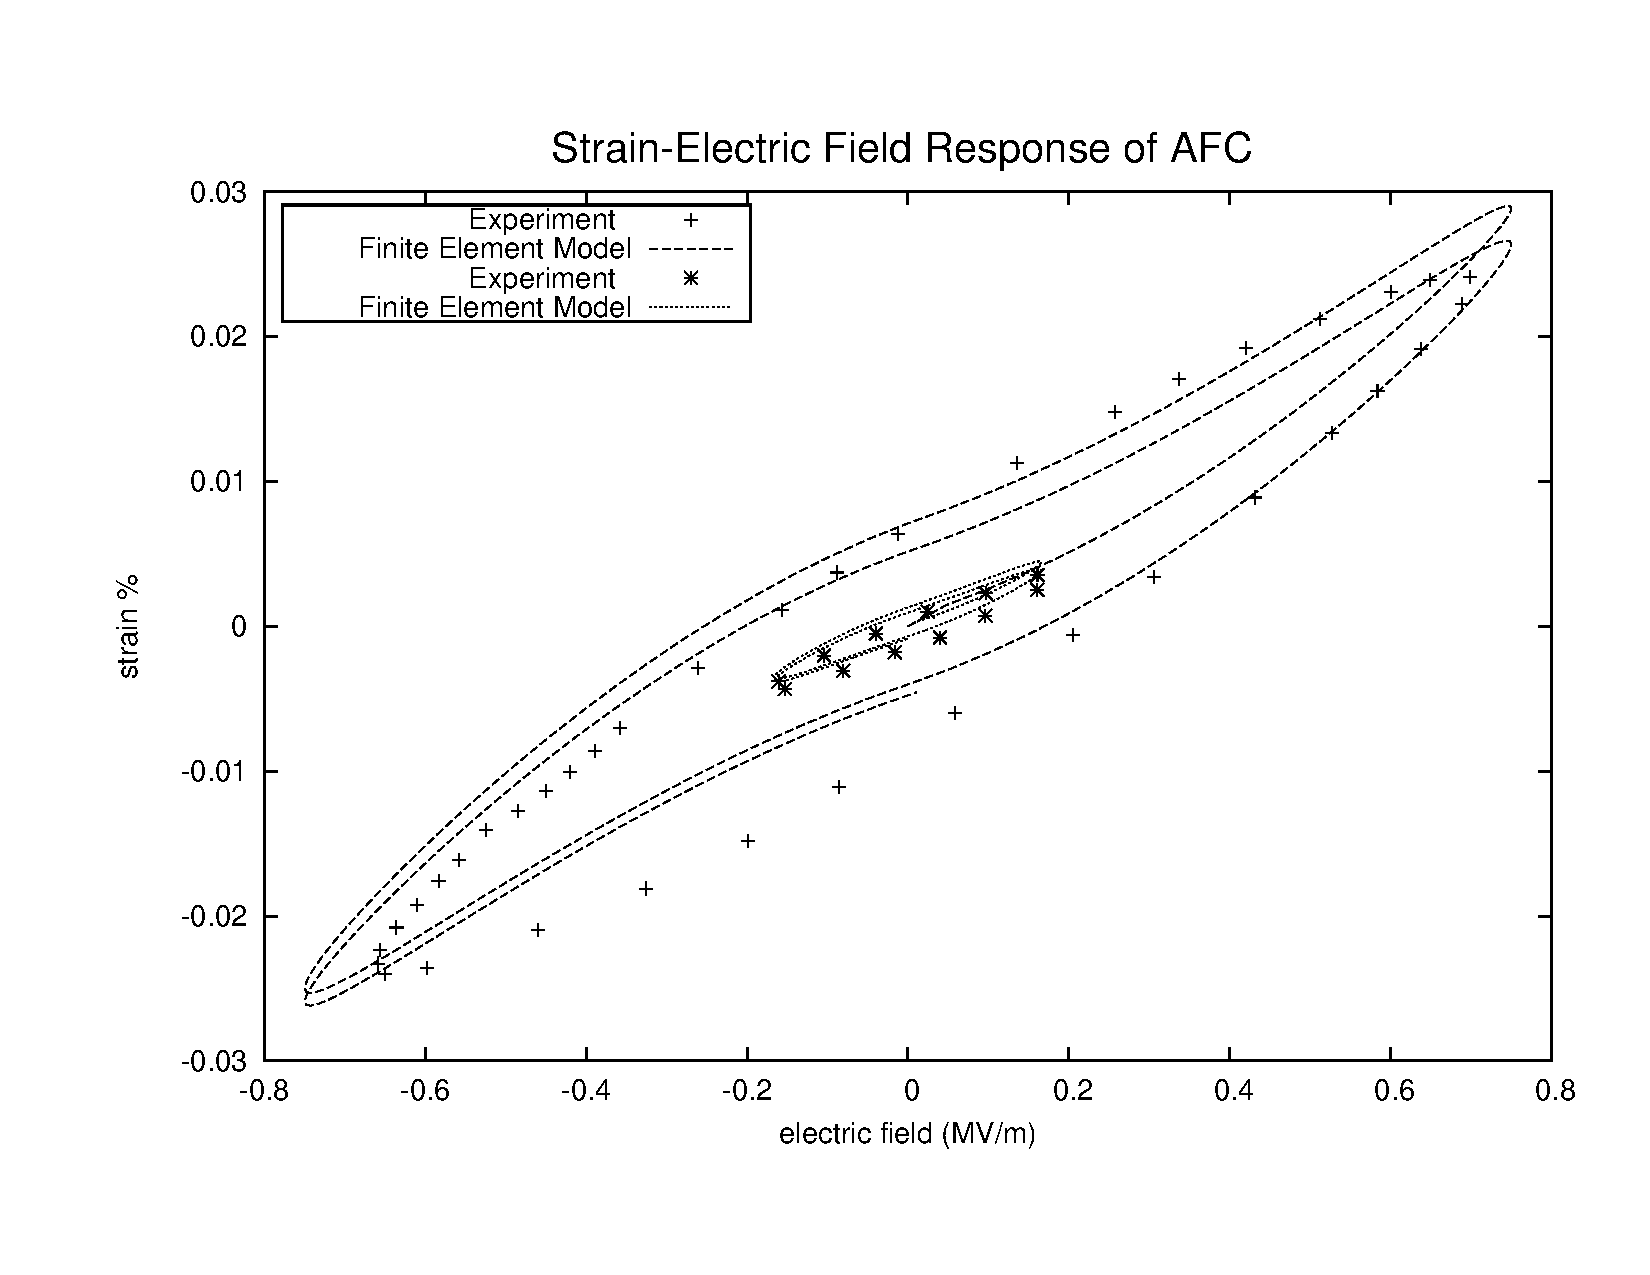
\includegraphics[trim = 0mm 0mm 0mm 0mm,width=5.0in]
{./chap_4_structural_analyses/afc_unit_cell/non_linear_hysteris_afc/non_linear_electric_field_vs_polarization.pdf}
\caption{Nonlinear electro-mechanical hysteresis for different electric fields at 1Hz compared with experiment}
\label{fig:non_linear_electric_field_vs_polarization}
\end{figure}

\subsection{The Effect of Scale Time on Electro Mechanical Response of AFC}
It can be shown that at higher intensity of electric field the piezoelectric materials respond faster to the change in electric field.
We use the same analogy with thermorheologically simple materials that have widely used for mechanical response of polymers \cite{haj2004numerical, tscharnuter2012nonlinear}.
The time scale factor is defined as an exponential function with respect to the electric field intensity $|\textbf {E}|$.
Then the reduced time is defined as:

\begin{equation}
	\phi(t) = \int_0^t \frac{ ds } { a_{( |\textbf {E}| } ) } 
\label{equation:time_scaling}	
\end{equation}
where ${a(|\textbf {E}|)}$ is the time shift factor that is defined in terms of then electric field vector:
 
\begin{equation}
a_{ |\textbf {E}| }=e^{-\gamma_{E} \times |\textbf {E}|}
\label{equation:time_scaling_factor}	
\end{equation}
where $\gamma$ is the material constant.
\begin{figure} 
\centering
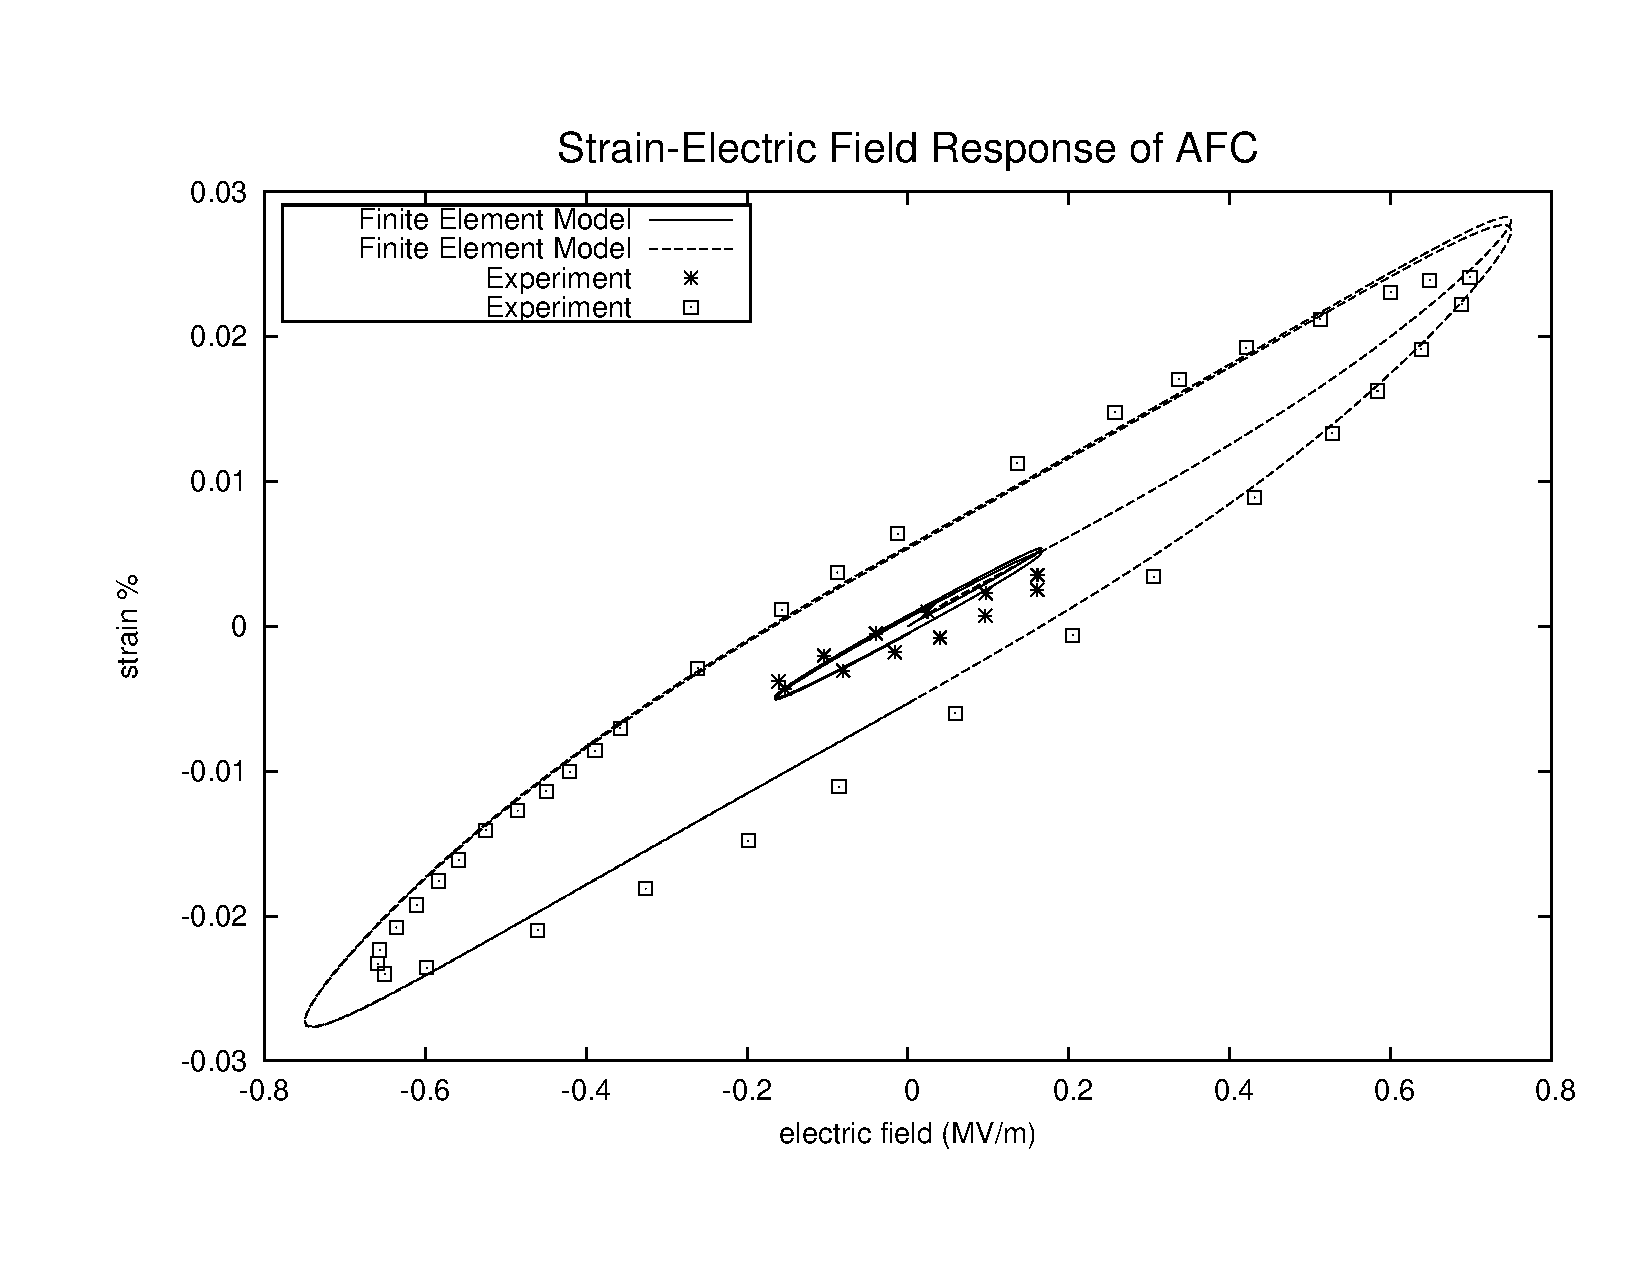
\includegraphics[trim = 0mm 0mm 0mm 0mm,width=5.0in]
{./chap_4_structural_analyses/afc_unit_cell/linear_hysteris_time_shift_afc/time_shift_afc_electric_field_vs_strains.pdf}
\caption{Linear electro-mechanical hysteresis response of AFC model with time shift for different electric fields at 1Hz compared with experiment}
\label{fig:time_shift_afc_electric_field_vs_strains}
\end{figure}

Figure \ref{fig:time_shift_afc_electric_field_vs_strains} shows the result of time-dependent analyses, including the time shift concept for piezoelectric materials.
The shift material constant is taken as $\gamma_{E}=1.75 m/MV$. 
Rests of the material properties are same as table  \ref{table:non_linear_materila_properties_afc}.
Except that for linear time dependent response of PZT5A $\widehat{b}_{3333}=0$ and ${}^{1}K_{ijk}^{e}=-0.6$ are taken.
Better predictions of the experimental data are observed.

% In order to examine the rate (frequency) dependent response, parametric studies are presented by applying electric fields at various frequencies. 
% The corresponding strains response of the model under different frequencies and amplitudes are shown in figure \ref{fig:afc_Frequency_Effect}. 
% It is apparent from the results that higher frequency and also very low frequency of loading reduces time-dependent (hysteresis) effect. 
% This is due to the fact that the material does not have enough time to exhibit time-dependent effect. 
% Fast loading reduces the creep-like or relaxation-like behavior and the area inside the hysteresis curve becomes smaller.


In order to examine the rate (frequency) dependent response, parametric studies are presented by applying electric fields at various frequencies. The corresponding strains response of the model under different frequencies and amplitudes are shown in figure \ref{fig:afc_Frequency_Effect}. It is apparent from the results that higher frequency and also very low frequency of loading reduces time-dependent (hysteresis) effect. This is because the process time (or duration of loading) in case of lower frequency loading is much longer than the characteristic creep/relaxation time in the material, while for high frequency loading, the process time is much faster than the characteristic time of the materials. In such situation, the effect of time associated with the creep/relaxation behavior is less significant. 

\begin{figure} 
\centering
\subcaptionbox{Frequency 0.1 Hz}
{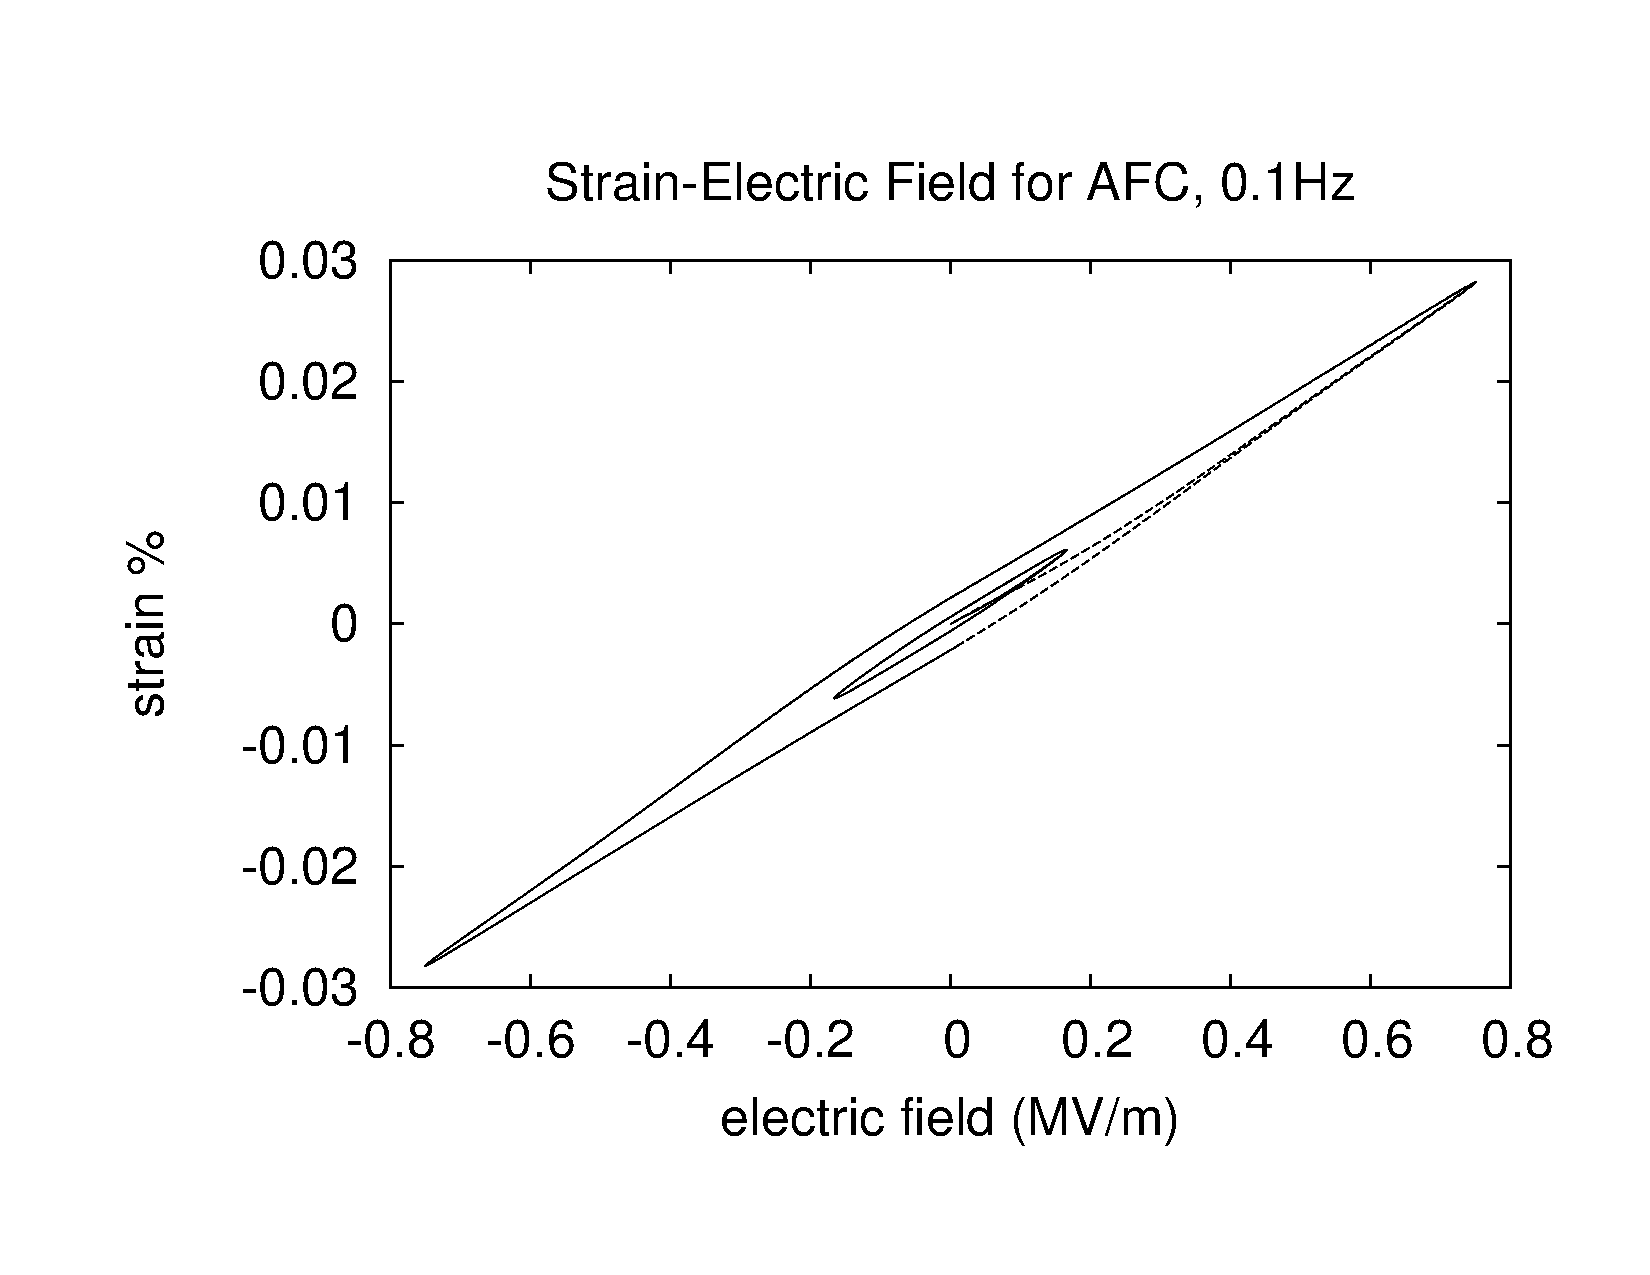
\includegraphics[width=2.9in]{./chap_4_structural_analyses/afc_unit_cell/frequency_effect/electric_field_vs_strains_freq_0p1}}
\subcaptionbox{Frequency 0.2 Hz}
{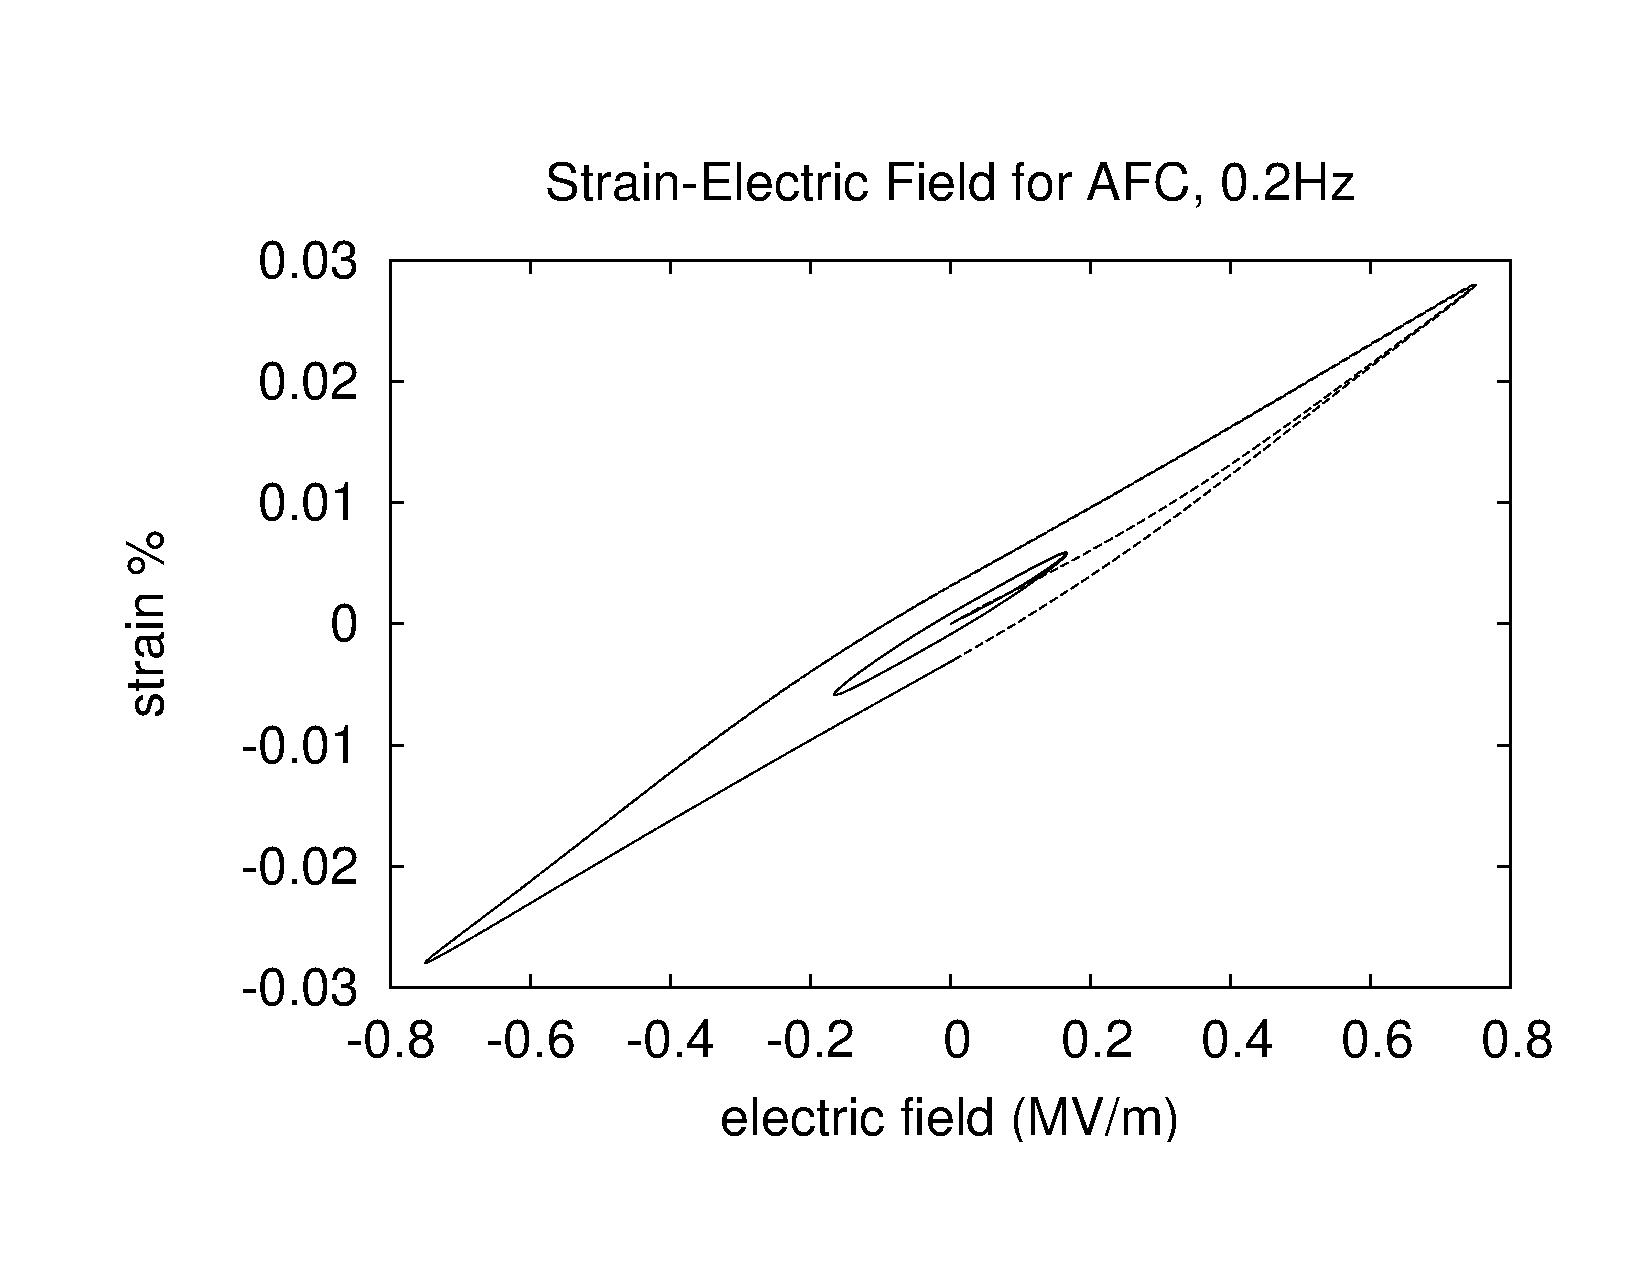
\includegraphics[width=2.9in]{./chap_4_structural_analyses/afc_unit_cell/frequency_effect/electric_field_vs_strains_freq_0p2}}
\subcaptionbox{Frequency 0.5 Hz}
{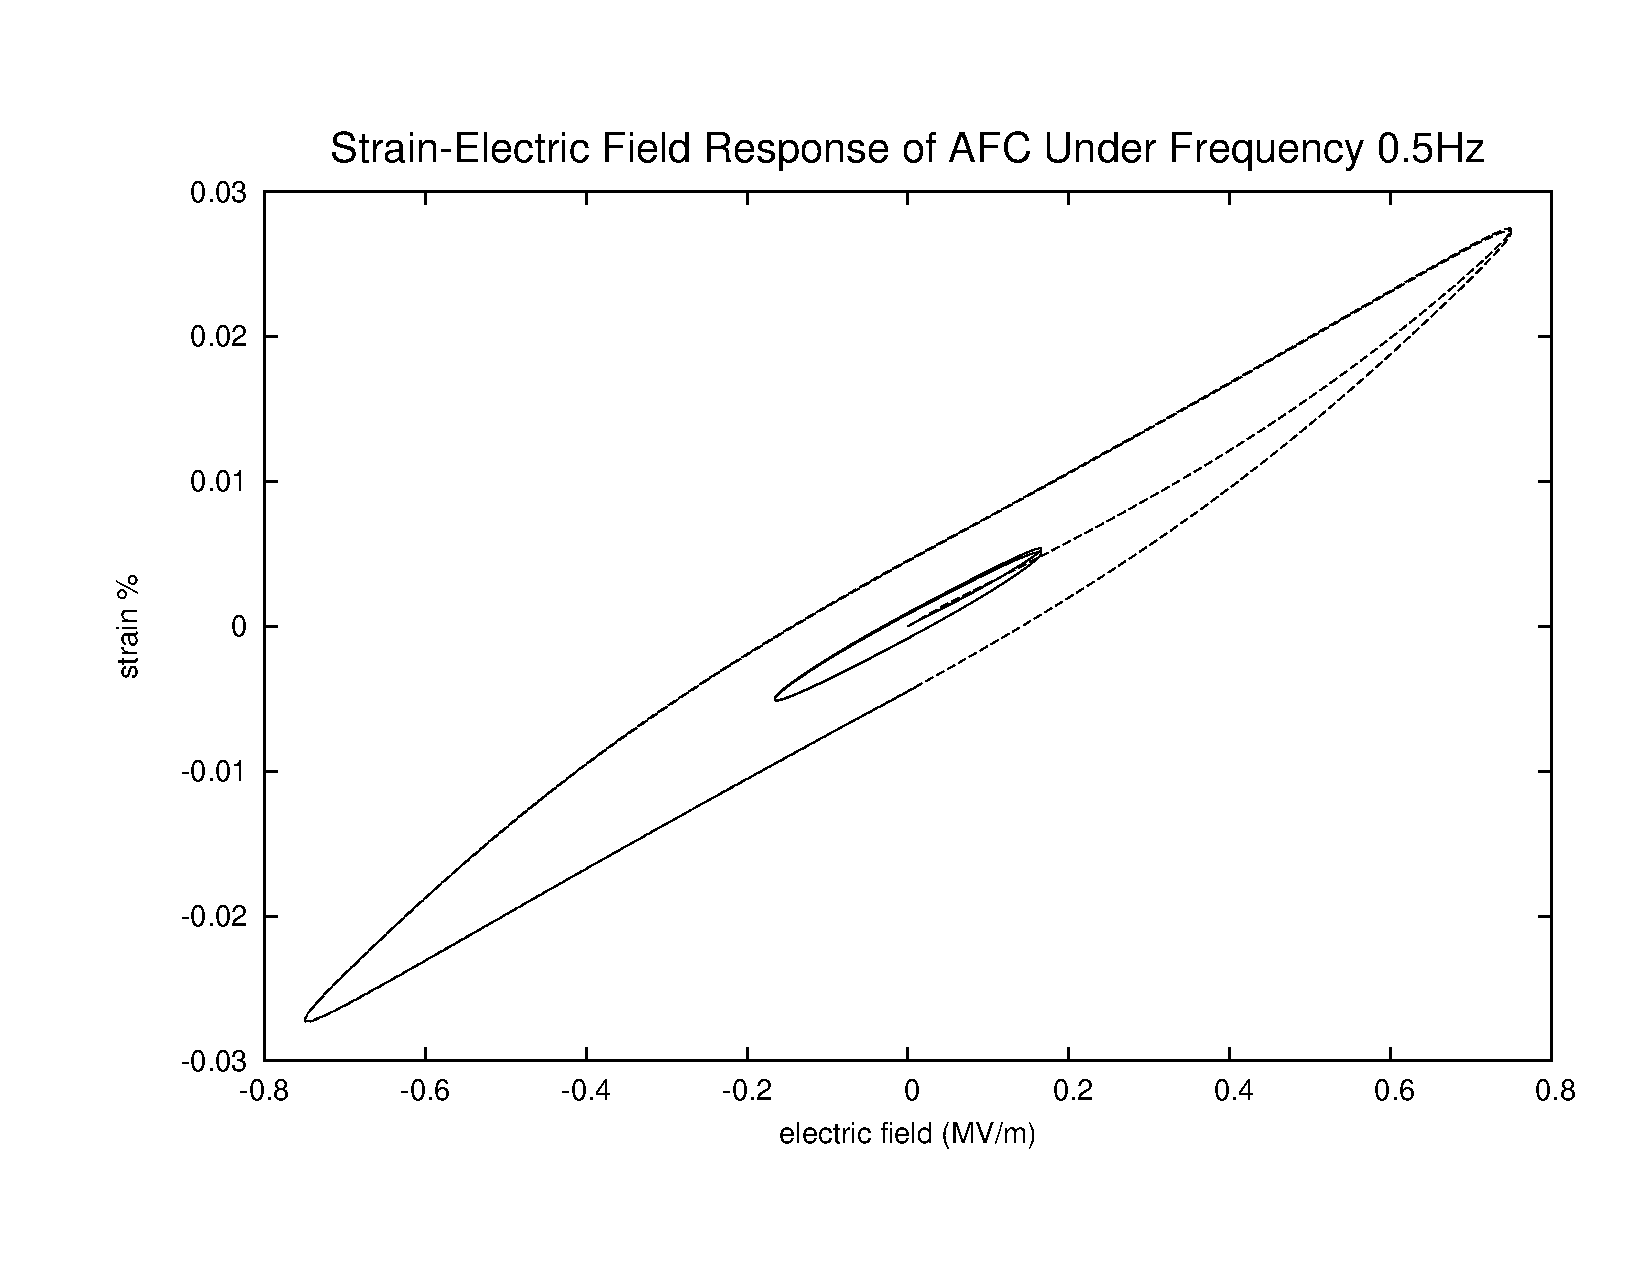
\includegraphics[width=2.9in]{./chap_4_structural_analyses/afc_unit_cell/frequency_effect/electric_field_vs_strains_freq_0p5}}
\subcaptionbox{Frequency 2.0 Hz}
{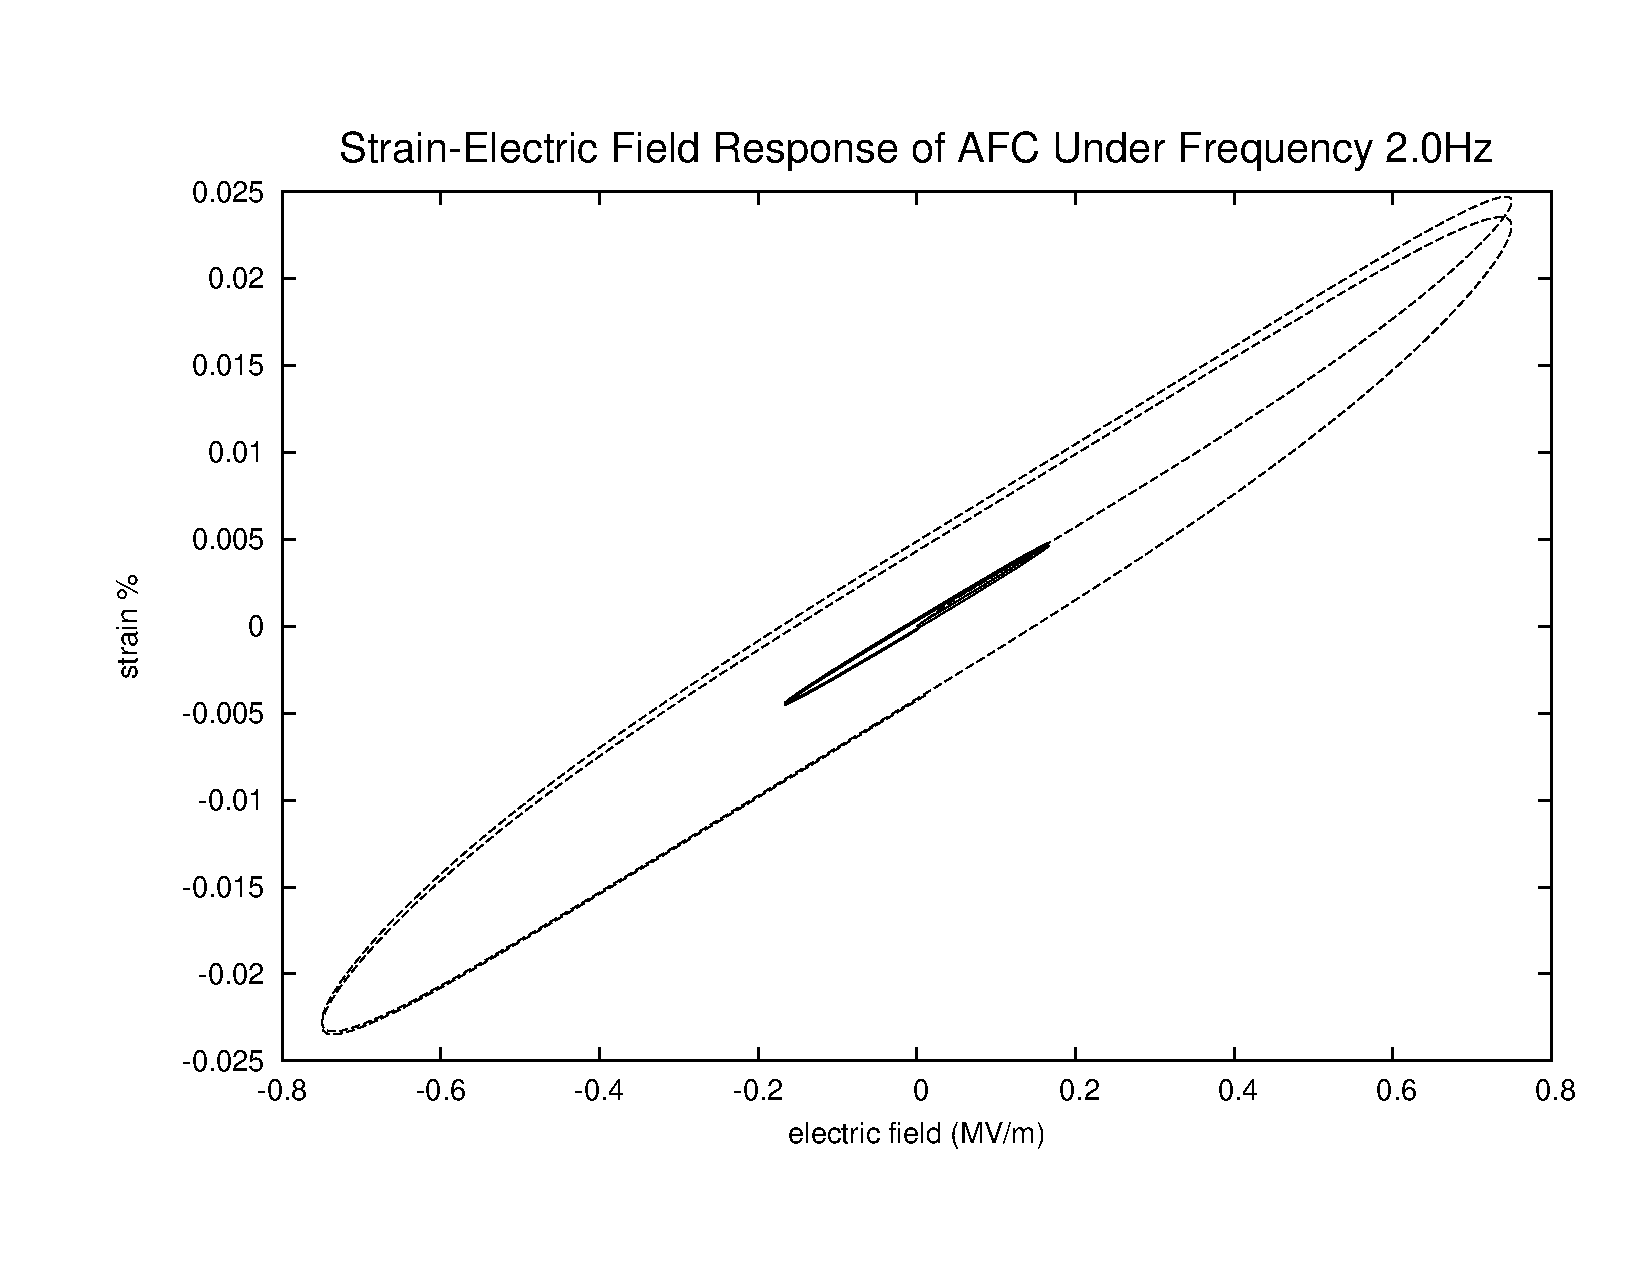
\includegraphics[width=2.9in]{./chap_4_structural_analyses/afc_unit_cell/frequency_effect/electric_field_vs_strains_freq_2p0}}
\subcaptionbox{Frequency 5.0 Hz}
{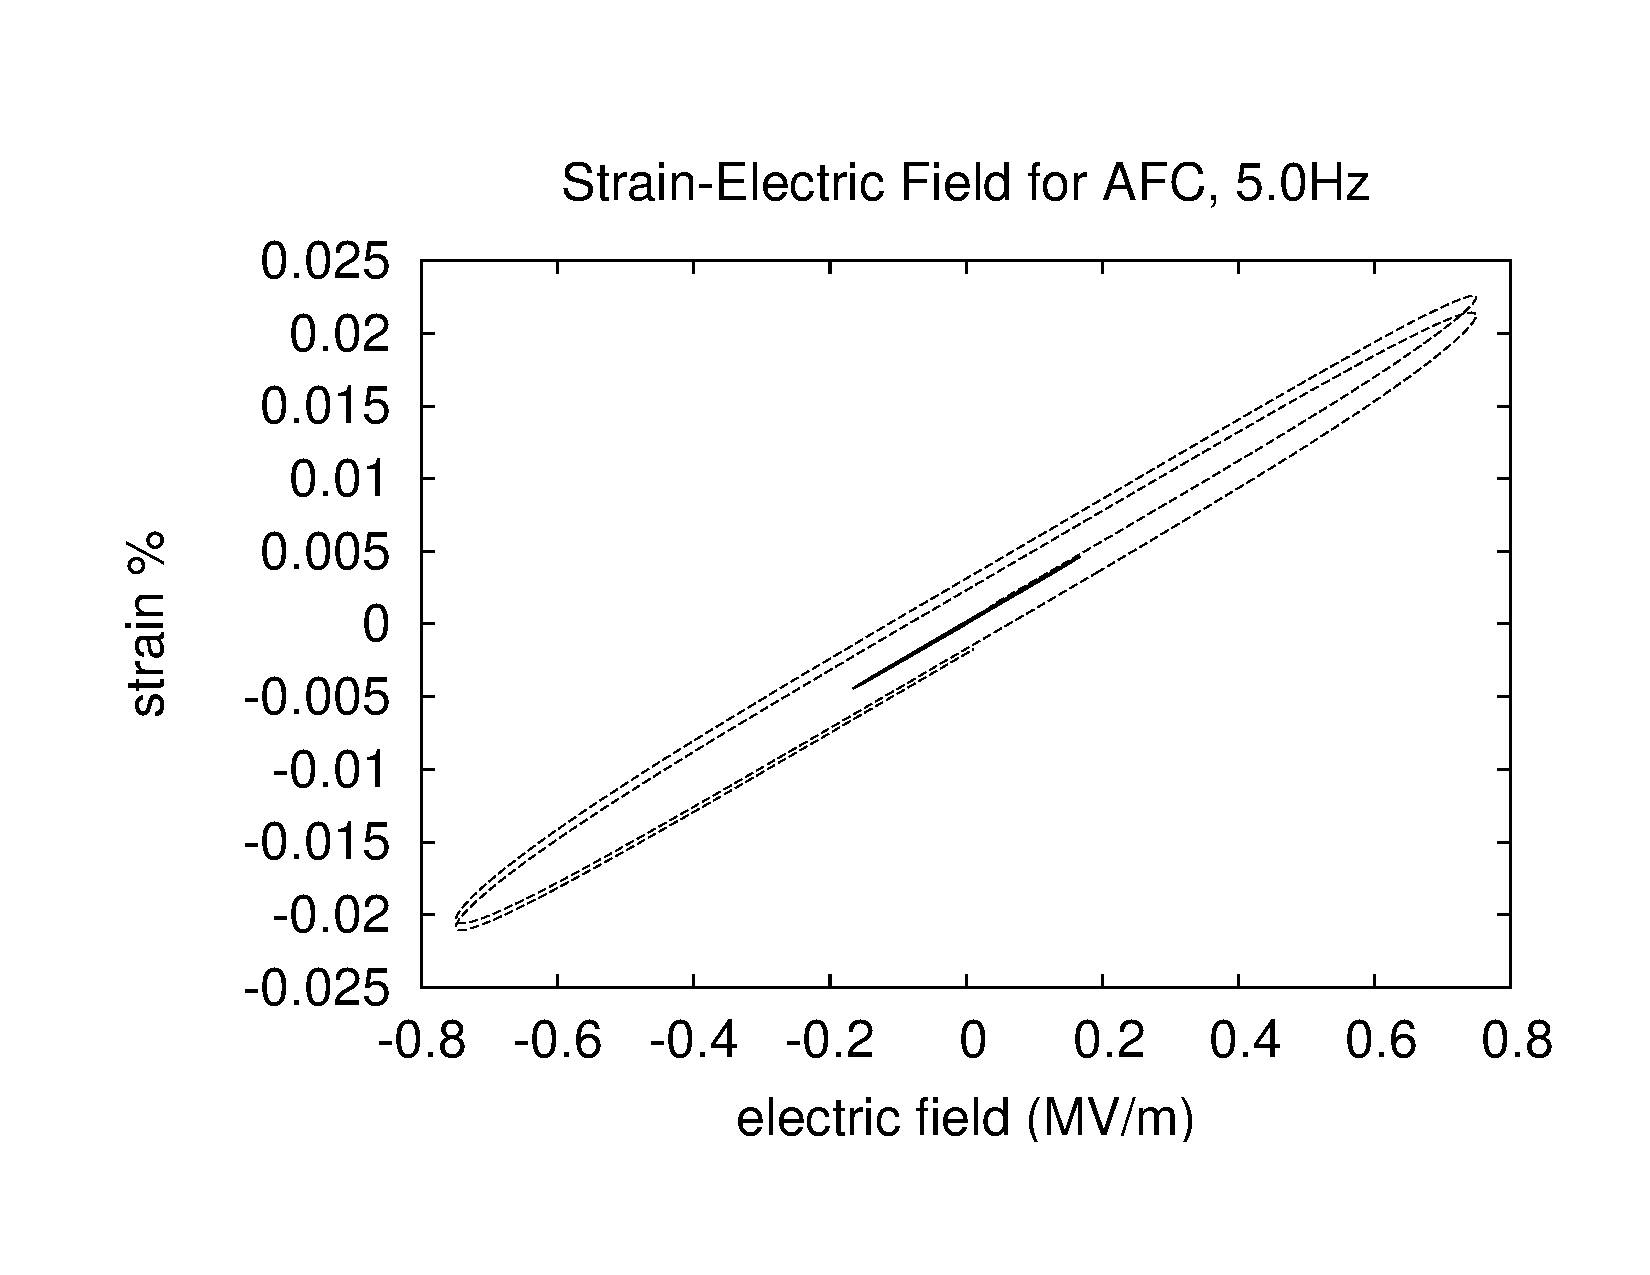
\includegraphics[width=2.9in]{./chap_4_structural_analyses/afc_unit_cell/frequency_effect/electric_field_vs_strains_freq_5p0}}
\subcaptionbox{Frequency 10.0 Hz}
{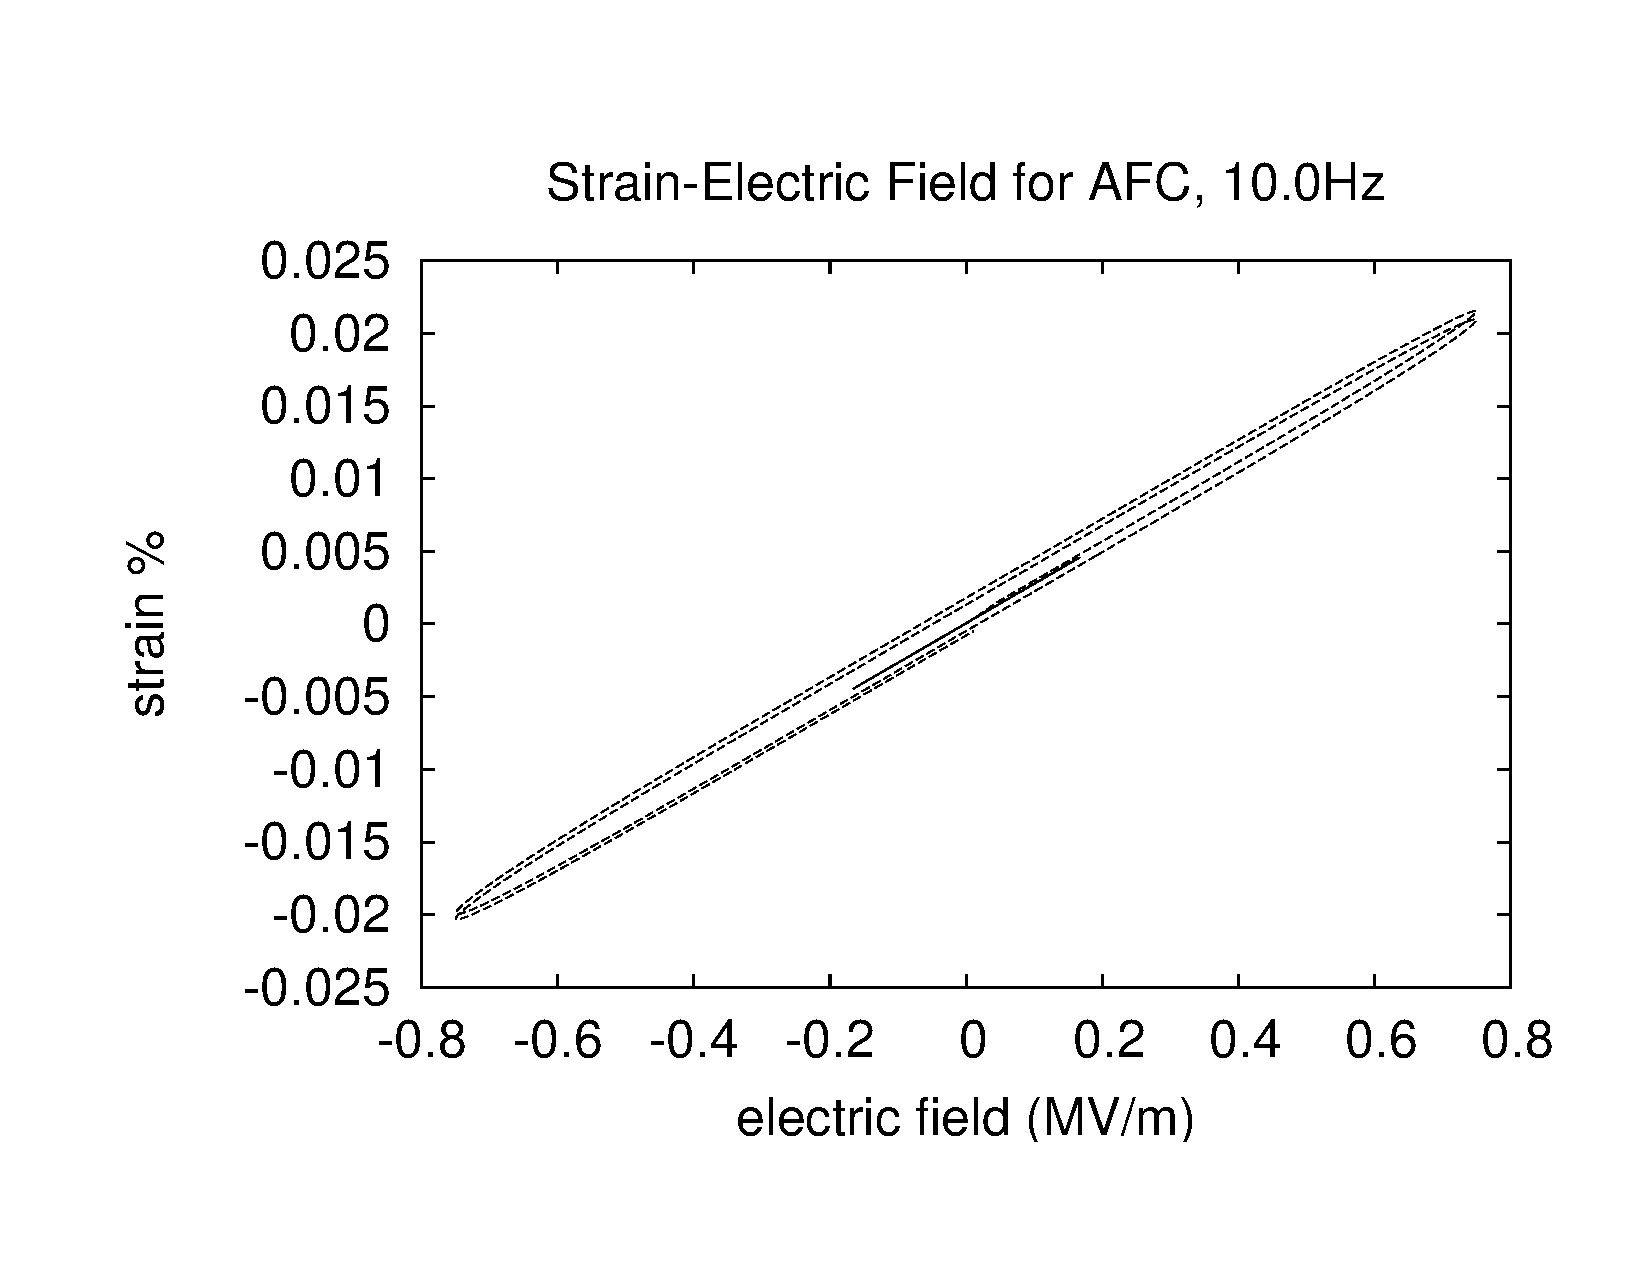
\includegraphics[width=2.9in]{./chap_4_structural_analyses/afc_unit_cell/frequency_effect/electric_field_vs_strains_freq_10p0}}
\caption{Effect of frequency of applied electric field on strain response of AFC}
\label{fig:afc_Frequency_Effect}
\end{figure}

% Figure \ref{afc_freq_xp_model:fig} shows Mechanical response of AFC model to different frequencies of applied electric field, compared with experiment  [2].
% Four Proney terms are used for electromechanical coupling coefficients of PZT fiber to capture response of model in different frequencies.
% The mechanical and electrical properties of afc model is shown in table \ref{table:afc_freq_xp_model:fig}.





Finally, responses of AFC at different frequencies are compared with available experimental data from Ben Atitallah \cite{atillah2014}. Figure \ref{afc_freq_xp_model:fig} shows the electro-mechanical responses of AFC at frequencies 0.2, 1, and 5 Hz under  applied electric field 0.6MV/m, compared with experiment \cite{atillah2014}. Four Prony terms are used for electromechanical coupling coefficients of PZT fiber to capture response of model at different frequencies. 
The mechanical and electrical properties of the constituents of AFC are shown in table \ref{table:afc_freq_xp_model:fig}. Reasonable response predictions are shown for the three frequencies considered. 



\begin{figure} 
\centering
\subcaptionbox{0.2Hz}
{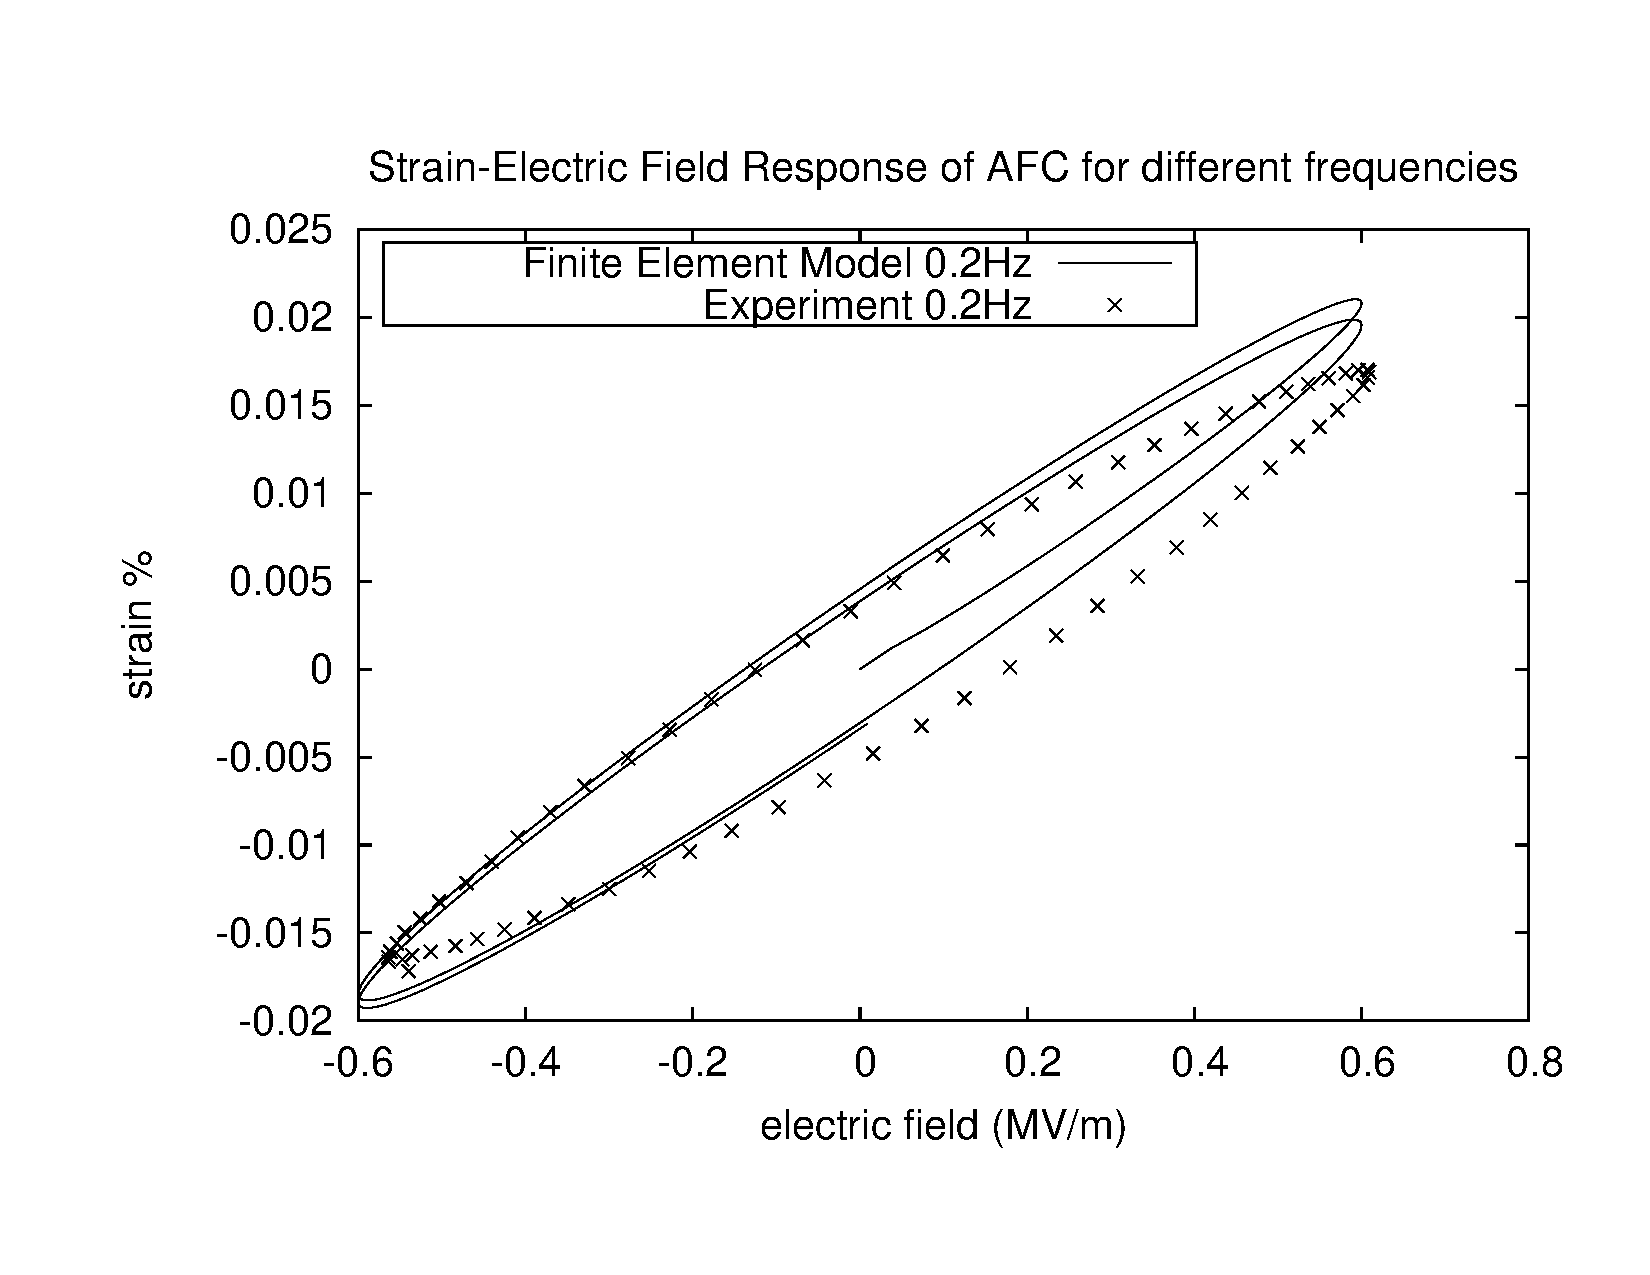
\includegraphics[width=3in]{./chap_4_structural_analyses/afc_unit_cell/wxp_different_frequencies/electric_field_vs_strains_for_different_frequencies_0p_2.pdf}}
\subcaptionbox{1.0Hz}
{\includegraphics[width=3in]{./chap_4_structural_analyses/afc_unit_cell/wxp_different_frequencies/electric_field_vs_strains_for_different_frequencies_1p_0.pdf}}
\subcaptionbox{5.0Hz}
{\includegraphics[trim = 0.5in 0in 0in 0in, clip, width=3in]{./chap_4_structural_analyses/afc_unit_cell/wxp_different_frequencies/electric_field_vs_strains_for_different_frequencies_5p_0.pdf}}
\caption{Mechanical response of AFC model to different frequencies of applied electric field, compared with experiment \cite{atillah2014}}
\label{afc_freq_xp_model:fig}
\end{figure}


\begin{table}
\caption{Material properties of AFC with four Prony series}
\centering
\begin{tabular}{ccccc} \hline
               & PZT5A & Epoxy & Aluminum & \\ \hline 
Young's Modulus&60.06 & 1.5     & 69       &$GPa$    \\ 
Poisson's Ratio&$0.3$ & 0.35    & 0.33 &\\  
$e_{113}$      &-12.7764 &         &      &$C/m^2$\\ 
$e_{311}$      &10.3935&         &      &$C/m^2$\\ 
$e_{333}$      &-24.5388  &         &      &$C/m^2$\\ 
$\kappa_{11}=\kappa_{22}$ &  $ 4  $ & $8.854  $ & &  pF/m \\ 
$\kappa_{33}$ & $2  $              & $8.854  $ & &  pF/m \\ 
${}^{0}K_{ijk}^{e}$&1.0& & &  \\ 
${}^{1}K_{ijk}^{e}$&-0.13& & & \\ 
${}^{2}K_{ijk}^{e}$&-0.30& & & \\ 
${}^{3}K_{ijk}^{e}$&-0.10& & & \\ 
${}^{4}K_{ijk}^{e}$&-0.26& & & \\ 
${}^{0}\lambda_{ijk}^{e}$&0& & & s \\ 
${}^{1}\lambda_{ijk}^{e}$&0.2& & & s \\  
${}^{1}\lambda_{ijk}^{e}$&1.0& & & s \\  
${}^{1}\lambda_{ijk}^{e}$&10& & & s \\  
${}^{1}\lambda_{ijk}^{e}$&60& & & s \\  
${}^{0}K_{ijkl}^{c}$& &1.0 & &  \\ 
${}^{1}K_{ijkl}^{c}$& &0.1 & & \\ 
${}^{0}\lambda_{ijkl}^{c}$& &0&  & s\\ 
${}^{1}\lambda_{ijkl}^{c}$& &0.8 & & s \\ \hline 
\end{tabular}
\label{table:afc_freq_xp_model:fig}
\end{table} 

\chapter{\uppercase{Active Trusses}}  
\label{section:chap_05_active_trusses} 
Simulations of shape changing in active truss structures are discussed in this chapter. Finite element analyses of 3D truss system are presented and both material and geometric nonlinearities are considered in the analyses. Two truss systems with cubical and tetrahedral arrangements of trusses as building blocks are considered in order to generate planar truss and longitudinal (beam like) truss systems, respectively. Shape changing in these truss systems is controlled by an actuation of each truss component using a piezoelectric actuation.
\\

\section{Deformed Shapes}  
Consider a 3D continuum object in a reference configuration $X_i$.
This continuum object changes its shape from the reference $X_i$ configuration to current configuration $x_i$.
In the case of Lagrangian description, the current configuration is defined as a function of reference configuration:

\begin{equation}  
x_i=\chi (X_i)   
\label{lagrangian_descriptoin} 
\end{equation}
Since the new configuration is decided a priori, the mapping function $\chi (X_i)$ is defined and the gradient of deformation is known:
\begin{equation}
F_{ij}=\frac{\partial x_i}{\partial X_j}
\label{deformation_gradient_tensor}
\end{equation}
The strain corresponding to the induced deformation in the truss system is easily calculated.  
The Green-St. Venant strain is given as:
\begin{equation}
E_{KL}=\frac{1}{2}\left( \frac{\partial x_j}{\partial X_K}\frac{\partial x_j}{\partial X_L}-\delta_{KL}\right)
\label{lagrange_green_strain}
\end{equation}
In order to induce the desired strain in each truss member associated with the shape change, an electric field is prescribed to the truss member. The deformation in each truss member is considered only along the longitudinal axis of each truss. Thus, the constitutive relation for each truss along its longitudinal axis is: 
\begin{equation}
E_{11}=f_1(S_{11})+f_2(E_3)
\label{one_constitutive_equation}
\end{equation}
where $E_{11}$ is the axial strain along the longitudinal axis of each truss member, $f_1(S_{11})$ is the strain due to the mechanical stress along the longitudinal axis of the truss $S_{11}$ and $f_2$ is the strain due to the electric field input, prescribed through the thickness of the truss, $E_3$.
In order to achieve desired shapes in the truss system, either stress or electric field, or both stress and electric field can be prescribed.
The longitudinal starin in each truss member is related to global strain of the by a transformation $Q_{ij}=N^{truss}_i N^{truss}_j$. 
This transformation is used to find the applied electric field in each member later in this chapter.
The constitutive relation for the truss is discussed later in this chapter.

\section{Nonlinear Truss Finite Element}
Truss systems consist of relatively slender members connected by pin joints.
The pin joints allow the members to rotate with respect to each other.
Each truss element is specified by two joints in the space and the shortest distance connects these two joints.
Let us consider two joints $P_1$ and $P_2$.
The locations of these two joints in the reference configuration are defined by two vectors namely $\mathbf {X^{P_1}}$ and $\mathbf {X^{P_2}}$.
The vector that connects these two joints in the reference configuration is defined as:
\begin{equation}
\mathbf {V^{12}=X^{P_2}-X^{P_1} } 
\end{equation}
and the base vector in the longitudinal direction of each truss member that connects these two joints is: 
\begin{equation}
\mathbf {N^{12}=V^{12}/ \|V^{12}\| }
\end{equation}
The displacement in the truss systems is defined in terms of a displacement of each node with respect to the reference configuration: 
\begin{equation}
u^{P_1}_i=x^{P_1}_i-X^{P_1}_i ; u^{P_2}_i=x^{P_2}_i-X^{P_2}_i ;  
\end{equation}
If linear test functions are used for the finite element approximation, the displacement at each point on the truss can be interpolated as a linear function. The master shape function of the isoparametric element $\zeta \in [-1,1]$ is introduced as:
\begin{equation}
\begin{aligned}
& \psi^1=0.5(1+\zeta); \psi^1_{,\zeta}= 0.5 \\
& \psi^2=0.5(1-\zeta); \psi^2_{,\zeta}=-0.5
\end{aligned}
\label{shape_function_truss} 
\end{equation}
The mapping must be defined from each truss element into this master element.
The global deformation gradient is:
\begin{equation}
\frac{\partial u_i}{\partial X_j}=\frac{\partial u_i}{\partial \zeta}
\frac{\partial \zeta}{\partial X_j}
\label{eqn:global_derivitave} 
\end{equation}
For the truss element in 3D the gradient of deformation is:
\begin{equation}
\frac{\partial X_j }{\partial \zeta}= 
  \sum_{i=1}^{NPE=2} \psi^i_{,\zeta} X^{P_i}_j 
\label{eqn:delXi_delzeta} 
\end{equation}
where NPE is the number of joints in an element.
It is noted that the integration is done on the member that connects two joints of the truss element.
Then the deformation gradient at a point on the truss is defined as:
\begin{equation}
F_{ij}=\delta_{ij}+ \frac{\partial u_i}{\partial X_j};  
\end{equation}
\\

\subsection{Space Filler Truss Configuration}
The first example that is considered is a planar truss.
The truss is formed by the cubical element as a building block. 
A single element that forms the truss system is shown in figure \ref{fig:cuber_space_filler_truss}.
The element consists of 12 side truss members and 4 diagonal members.
The deformation of the members can be controlled by the electric field or other stimuli.
The change in the length of each member will cause change of shape of each single cubical element and consequently change in shape of the structure that is made of these members.

\begin{figure} 
\centering
\includegraphics[width=5.0in]{./chap_5_active_trusses/images_space_filler/cube.png}
\caption{One element of space filler truss}
\label{fig:cuber_space_filler_truss}
\end{figure}

As an example, consider a planar domain that is in the form of a plate structure.
The domain is defined as follows:

\begin{equation}
\begin{aligned}
X_1 \in & [-L_1/2,L_1/2] \\
X_2 \in & [-L_2/2,L_2/2] \\
X_3 \in & [-h/2,h/2]
\end{aligned}
\label{planar_truss_domain:eqn}
\end{equation}
 
Let us first consider $[L_1,L_2,h]=[1,1,0.1]$ unit is in meter, and fill the domain with 20x20 elements in $X_1$ and $X_2$ directions and 1 element in $X_3$ direction. 
The planar truss is shown in figure \ref{fig:planar_truss_ref_config}.  
If the truss system is intended to have a shape as is shown in figure \ref{fig:xy_plane_desired_shape} the mapping between the reference and current configurations for $X_3=X_1 X_2$ surface is defined as follows.

\begin{figure} 
\centering
\includegraphics[width=5.0in]{./chap_5_active_trusses/images_space_filler/planar_truss_ref_config.png}
\caption{Planar Truss in Reference Configuration}
\label{fig:planar_truss_ref_config}
\end{figure}

\begin{figure} 
\centering
\includegraphics[width=5.0in]{./chap_5_active_trusses/images_space_filler/xy_plane_desired_shape.jpg}
\caption{The desired current configuration for the planar truss}
\label{fig:xy_plane_desired_shape}
\end{figure}

\begin{equation}
\begin{aligned}
x_1(X_1,X_2,X_3) = & X_1 \\
x_2(X_1,X_2,X_3) = & X_2 \\
x_3(X_1,X_2,X_3) = & X_3+X_1 X_2 \\
\end{aligned}
\label{doubly_curved_mapping:eqn}
\end{equation}
The deformation gradient for this above mapping function is defined as:
\begin{equation}
\mathbf F=
\begin{bmatrix}
1&0&0 \\
0&1&0 \\
X_2 & X_1 & 1
\end{bmatrix}
\label{deformation_gradient_doubly_curved_mapping:eqn}
\end{equation}

Then the stretch tensor $\mathbf C=\mathbf {F^T F}$ and Green-St. Venant strain tensors are:

\begin{equation}
\mathbf C=
\begin{bmatrix}
X_{2}^2+1&X_{1}\,
X_{2}&X_{2}\cr X_{1}\,X_{2}&X_{1}^2+1&X_{
 1}\cr X_{2}&X_{1}&1\cr 
\end{bmatrix}
; \mathbf E=
\begin{bmatrix}
X_{2}^2&X_{1}\,X_{2}&X_{2}\cr X_{1}\,X_{2}&X_{1}^2&X_{1}\cr X_{2}&X_{1}&0\cr 
 \end{bmatrix}
\label{green_deformation_tensor_doubly_curved_mapping:eqn}
\end{equation} 
  
\begin{figure} 
\centering
\includegraphics[width=5.0in]{./chap_5_active_trusses/images_space_filler/planar_truss_deformed_config.png}
\caption{The deformed configuration for the planar truss}
\label{fig:planar_truss_deformed_config}
\end{figure}

It is shown in figure \ref{fig:planar_truss_deformed_config} that the application of electric stimuli to each truss member can induce desired shape. The space filler truss that has been discussed in the previous chapter can offer good flexibility for planar and even 3D shapes. 

Another shape that is considered for the planar truss is the saddle point surface.
The shape $X_3=X_1^2-X_2^2$ is induced in the planar truss with the same procedure that is already described.
If we assume that truss member are made of electro active materials with overall electromechanical coupling coefficient as $d_{311}^0=340pm/V$ the corresponding required electric field contour for each truss will be as in figure \ref{fig:planar_z_eq_x2_y2_efield_contour}.
The strain induced in each truss for this truss configuration in shown in figure \ref{fig:planar_z_eq_x2_y2_strain_contour}.

\begin{figure} 
\centering
\includegraphics[width=5.0in]{./chap_5_active_trusses/images_space_filler/planar_truss_z_eq_x2_y2_strain.png}
\caption{The strain contour of planar space filler truss for the $X_3=X_1^2-X_2^2$ shape (displacement are scaled 20 times)}
\label{fig:planar_z_eq_x2_y2_strain_contour}
\end{figure} 

\begin{figure} 
\centering
\includegraphics[width=5.0in]{./chap_5_active_trusses/images_space_filler/planar_truss_z_eq_x2_y2_elec_field.png}
\caption{The electric field contour of planar space filler truss for the $X_3=X_1^2-X_2^2$ shape (displacement are scaled 20 times)}
\label{fig:planar_z_eq_x2_y2_efield_contour}
\end{figure} 


% XXXXXXXXXXXXXXXXXXXXXXXXXXXXXXXXXXXXXXXXXXXXXX.
 
\subsection{Tetrahedral Beam Like Truss}
Using a tetrahedral shape as a building block for truss configurations it is possible to form the longitudinal truss elements to take a beam like form. The building block of the tetrahedral beam like truss is shown in figure \ref{fig:building_block_of_tetrahedral_truss} that contains 3 tetrahedral.
\begin{figure} 
\centering
\includegraphics[width=5.0in]{./chap_5_active_trusses/images_linear_tetrahedral/building_block_of_tetrahedral_truss.png}
\caption{The building block of tetrahedral beam like truss}
\label{fig:building_block_of_tetrahedral_truss}
\end{figure} 
The beam like truss is formed by arranging these tetrahedral units in one direction.
An example of truss with 150 tetrahedral units is shown in figure \ref{fig:refrence_shap_100_tetra_unit_tetrahedral_unit}. 
\begin{figure} 
\centering
\includegraphics[width=5.0in]{./chap_5_active_trusses/images_linear_tetrahedral/refrence_shap_100_tetra_unit_tetrahedral_unit.png}
\caption{Tetrahedral beam like truss with 150 Units that is Used as Reference Configuration}
\label{fig:refrence_shap_100_tetra_unit_tetrahedral_unit}
\end{figure} 

It can be seen form the cross section view of the beam in figure \ref{fig:refrence_shap_100_tetra_unit_tetrahedral_unit_cross_section_view} that none of the truss members crosses the center line.   
Therefore, this configuration behaves like a hollow beam. 
Several examples of bending deformations are considered for the truss system.
The bending can be induced by creating normal strain in the axial direction of the truss members along the longitudinal axis of the beam.
In the simple bending case the radius of curvature of the beam $r_{curvature}$ is defined:
\begin{equation}
\begin{aligned}
r_{curvature}&=\frac{ L_{beam} }{2 \theta}\\
E_{11}&=X_3/r_{curvature}
\end{aligned}
\label{stran_and_radios_of_curvture_of_beam:eqn}
\end{equation}

\begin{figure} 
\centering
\includegraphics[width=5.0in]{./chap_5_active_trusses/images_linear_tetrahedral/refrence_shap_100_tetra_unit_tetrahedral_unit_cross_section_view.png}
\caption{Cross Section View of Tetrahedral beam like Truss (perspective view)}
\label{fig:refrence_shap_100_tetra_unit_tetrahedral_unit_cross_section_view}
\end{figure}

where 
$\theta$ is the curvature angle (for full circle it is $2\pi$) and
$ L_{beam}$ is the length of the beam made of tetrahedral units.
The strain $E_{11}=X_3/r_{curvature}$ causes lateral deformation in the $X_3$ direction with positive curvature.

We try to produce the shape of an arc with a curvature angle $\pi$.
The result is shown is figure \ref{fig:tetra_hedral_arc_pi_shape}.
As can be seen the shape is quite different from the real arc.
The reason of the difference between the produced shape and desired shape is due to disregarding the normal strain in the thickness direction of beam that is produced in bending of a beam.
Increasing the curvature in the tetrahedral beam like truss will cause a sinusoidal like shape in the truss.
The strain that is induced in this truss is taken from equation (\ref{stran_and_radios_of_curvture_of_beam:eqn}) with $\theta=2 \pi$.

\begin{figure} 
\centering
\includegraphics[width=5.0in]{./chap_5_active_trusses/images_linear_tetrahedral/tetra_hedral_arc_pi_shape.png}
\caption{Arc shape produced in the tetrahedral beam like truss}
\label{fig:tetra_hedral_arc_pi_shape}
\end{figure}  


\begin{figure} 
\centering
\includegraphics[width=5.0in]{./chap_5_active_trusses/images_linear_tetrahedral/tetra_hedral_arc_2_pi_shape.png}
\caption{Cyclic shape produced in the tetrahedral beam like truss}
\label{fig:tetra_hedral_arc_2_pi_shape}
\end{figure} 

In order to get a shape closer to the actual bending of a beam we then apply the normal strain in the thickness direction.
This will cause a strain of the field closer to the strain beam made of continuous solid members.
We modify the bending strain defined in equation (\ref{stran_and_radios_of_curvture_of_beam:eqn}) with the through thickness normal strain as follows:

\begin{equation}
\begin{aligned}
E_{11}&=X_3/r_{curvature}+\kappa_v \\
E_{22}&=-X_3/(2r_{curvature})+\kappa_v \\
E_{33}&=-X_3/(2r_{curvature})+\kappa_v
\end{aligned}
\label{strain_with_dilation:eqn}
\end{equation}
where $\kappa_v$ is the dilation that is added to mimic the effect of change in volume in the beam.
It is observed that if $\kappa_v=2.0$ there will be an arc forming in the beam like truss.
This arc is shown in figure \ref{fig:tetra_hedral_arc_2_pi_shape_with_pressure}.
\begin{figure} 
\centering
\includegraphics[width=5.0in]{./chap_5_active_trusses/images_linear_tetrahedral/tetra_hedral_arc_2_pi_shape_with_pressure.png}
\caption{Shape produced in the tetrahedral beam like truss including the all normal strains}
\label{fig:tetra_hedral_arc_2_pi_shape_with_pressure}
\end{figure} 

In the last example we will try to apply a shape in the beam in the way that it passes four specific points.
Consider bending of a tetrahedral beam like truss in the way that it passes through three points as follows:
\begin{equation}
\begin{aligned}
\underline X ^1&=(0,0,0) \\
\underline X ^2&=(L_{beam}/4,0,L_{beam}/8) \\
\underline X ^3&=(3 L_{beam}/4,0,-L_{beam}/8) \\
\underline X ^4&=(L_{beam},0,L_{beam}/8)
\end{aligned}
\label{three_points:eqn}
\end{equation}

In this case it can be found that the following strain should be applied:

\begin{equation}
E_{11}=X_3 \left(
\frac{329}{36L_{beam}} -
\frac{220 X_1}{L_{beam}^2} +
\frac{280 X_1}{ 3 L_{beam}^3}  \right)
\label{three_points_strain:eqn}
\end{equation}


\begin{figure}
\centering
\fbox{\includegraphics[width=5.0in]{./chap_5_active_trusses/truss_image_three_point/current_tetra_beamthree_point}}
\fbox{\includegraphics[width=5.0in]{./chap_5_active_trusses/truss_image_three_point/curve_beam-eps-converted-to_three_point}}
\caption{Shape of tetrahedral beam that passes thought four specific points}
\label{fig:tetra_hedral_three_point}
\end{figure}

\subsection{Effect of Nonlinear and Time Dependent Constitutive Equation on Active Truss}
By prescribing the above calculated strain field to the truss structure, the desired shape is attained. The corresponding strain in each truss element is achieved through applications of electric field to the piezoelectric materials in the truss members.
In the case of piezoelectric patch with the electro-mechanical coupling factor $d_{311}$ the electric field that should be applied to each truss $E_3$ can be found from the following equation:

\begin{equation}
\begin{aligned}
E_{11}^{truss} &=\sum_{i=1}^3 \sum_{j=1}^3 E_{ij}N^{truss}_i N^{truss}_j\\
E_{11}^{truss} &=E_3 d_{311} 
\end{aligned}
\label{electric_field_in_each_truss:eqn}
\end{equation}
where 
$N^{truss}$ is the vector in the direction of each truss element and 
$E_3$ is the electric field that should be applied to each truss element to induce the deformation.
When a nonlinear electro-mechanical constitutive equation is considered, the strain in the longitudinal axis of each truss is a nonlinear equation.
The relationship between the strain and electric field can also be taken as time dependent to include hystersis response of piezoelectric materials.

The effect of nonlinear and time dependent electro-mechanical response of each truss member on the overall deformation of truss structure is examined.
The time dependent constitutive equation based on quasi linear viscoelastic model that was introduced in previous chapters is used.
The tetrahedral truss system is used for these analyses and the desired shape is taken to be an arc with arc angle of $\pi/2$.
The strain distribution for this configuration is shown in figure \ref{fig:linear_tetrahedral_bending_strain_contour}.
\begin{figure} 
\centering
\includegraphics[width=5.0in]{./chap_5_active_trusses/images_non_linear_time_dependent_constitutive_equatio/linear_tetrahedral_bending_strain_contour.png}
\caption{The strain distribution in a beam like tetrahedral truss in the arc configuration}
\label{fig:linear_tetrahedral_bending_strain_contour}
\end{figure} 
If we take the electromechanical coupling factor as $d_{311}^0=340pm/V$ the corresponding required electric field contour for each truss shape is shown in figure \ref{fig:linear_tetrahedral_bending_efield_contour}.

\begin{figure} 
\centering
\includegraphics[width=5.0in]{./chap_5_active_trusses/images_non_linear_time_dependent_constitutive_equatio/linear_tetrahedral_bending_electric_field_contour.png}
\caption{The electric field distribution in a beam like tetrahedral truss in the arc configuration}
\label{fig:linear_tetrahedral_bending_efield_contour}
\end{figure} 

At first the analyses is conducted for a linear constitutive model for the truss.
The coupling between the stimuli and strain in the truss members are taken to be linear and independent of time.
The relationship between the input stimuli and maximum deflection in the middle of beam like tetrahedral beam in this analyses is shown in figure \ref{fig:linear_static_stimuli_vs_displacement}.
The stimulus is applied to each truss member with the frequency of 1Hz.

\begin{figure} 
\centering
\includegraphics[width=5.0in]{./chap_5_active_trusses/images_non_linear_time_dependent_constitutive_equatio/linear_static_stimuli_vs_displacement.pdf}
\caption{linear and time independent model for deflection under frequency 1Hz}
\label{fig:linear_static_stimuli_vs_displacement}
\end{figure} 

The nonlinear relationship between the deflection and input stimuli that is shown in figure \ref {fig:linear_static_stimuli_vs_displacement} is mainly due to geometric nonlinearity.

In case the time dependent electro-mechanical response, a cyclic electric field input with frequency 1Hz is prescribed.
The time kernel function with 
$K(t)=1.0-0.6 exp(-t/1.2)$ is considered within the integral representation for the strain 
$\varepsilon_{11}(t)=\int_0^t
K(t-s)\frac{\partial \varepsilon_{11}}{\partial E_3}\frac{\partial
E_3(s)}{\partial s} ds$ 
with 
$\frac{\partial \varepsilon_{11}}{\partial
E_3}=-d_{311}$ 
taken to be 
$340 pm/V$.
The hysteresis between the input stimuli and deflection is shown in figure \ref{fig:linear_tetrahedral_time_dependent_efield_vs_displacement}.

\begin{figure}  
\centering
\includegraphics[width=5.0in]{./chap_5_active_trusses/images_non_linear_time_dependent_constitutive_equatio/linear_tetrahedral_time_dependent_efield_vs_displacement.pdf}
\caption{linear and time dependent response for deflection under frequency 1Hz}
\label{fig:linear_tetrahedral_time_dependent_efield_vs_displacement}
\end{figure} 

We follow the same approach as previous chapters and assume the nonlinear and time dependent response for the constitutive equation in each truss element.
We define a nonlinear response function $\varepsilon_{11}(E_3)=-d_{311}^0 E_3-d_{311}^1 |E_3| E_3$.
Here we take $d_{311}^0=340pm/V$ and\footnote{$f$ here stands for femto i.e. $10^{-15}$ } $d_{311}^1=0.02 fm^2/V^2 $.
The results from taking a nonlinear and time dependent electric coupling between electric stimuli and resulting strain is shown in figure \ref{fig:linear_tetrahedral_time_dependent_efield_vs_displacement_nonlinear}.
The hysteresis curve shown in figure \ref{fig:linear_tetrahedral_time_dependent_efield_vs_displacement_nonlinear} combines the nonlinear response both from the large geometry and also from the nonlinear electro-mechanical constitutive in each truss. 

\begin{figure}   
\centering
\includegraphics[width=5.0in]{./chap_5_active_trusses/images_non_linear_time_dependent_constitutive_equatio/linear_tetrahedral_time_dependent_efield_vs_displacement_nonlinear.pdf}
\caption{nonlinear and time dependent response for deflection of beam like truss under frequency 1Hz}
\label{fig:linear_tetrahedral_time_dependent_efield_vs_displacement_nonlinear}
\end{figure} 

In figure \ref{fig:linear_tetrahedral_time_dependent_efield_vs_displacement_nonlinear_snapshot} the configuration of the truss in four different values of electric stimuli is shown.


\begin{figure}
\begin{subfigure}{.5\textwidth}
  \centering
  \includegraphics[width=.8\linewidth]{./chap_5_active_trusses/images_non_linear_time_dependent_constitutive_equatio/linear_tetrahedral_bending_snapshop_A.png}  
  \label{fig:sfigA}
\end{subfigure}%
\begin{subfigure}{.5\textwidth}
  \centering
  \includegraphics[width=.8\linewidth]{./chap_5_active_trusses/images_non_linear_time_dependent_constitutive_equatio/linear_tetrahedral_bending_snapshop_B.png}
  
  \label{fig:sfigB}
\end{subfigure}

\begin{subfigure}{.5\textwidth} 
  \centering
  \includegraphics[width=.8\linewidth]{./chap_5_active_trusses/images_non_linear_time_dependent_constitutive_equatio/linear_tetrahedral_bending_snapshop_C.png}
  \label{fig:sfigC}
\end{subfigure}%
\begin{subfigure}{.5\textwidth}
  \centering
  \includegraphics[width=.8\linewidth]{./chap_5_active_trusses/images_non_linear_time_dependent_constitutive_equatio/linear_tetrahedral_bending_snapshop_D.png}
  \label{fig:sfigD}
\end{subfigure}
\caption{The snapshots of linear tetrahedral truss in configurations labeled in figure \ref{fig:linear_tetrahedral_time_dependent_efield_vs_displacement_nonlinear}}
\label{fig:linear_tetrahedral_time_dependent_efield_vs_displacement_nonlinear_snapshot}
\end{figure}


As it can be seen from figures \ref{fig:linear_tetrahedral_bending_strain_contour} and \ref{fig:linear_tetrahedral_bending_efield_contour} the applied strain and therefore electric field can be beyond the limits of material. With a little investigation on the location of the maximum strain, it has been shown that even with the limiting amount of strain it is still possible to get the same shape.

The 1\% strain is chosen as maximum applicable strain.
As a result of limiting strain the resulting shape will change slightly.
The resulting shape with this limiting strain is shown in figure \ref{fig:limiting_strain_linear_tetrahedral_bending_strain_contour}.
Moreover, less electric field will be needed for the actuation as it is shown in figure \ref{fig:limiting_strain_linear_tetrahedral_bending_electric_field_contour}. 
Application of limiting strain in the model will decrease the maximum overall deflection of truss.
This will also change the shape of hysteresis curve as shown in figure  \ref{fig:limiting_strain_linear_tetrahedral_time_dependent_efield_vs_displacement_nonlinear}.

\begin{figure}  
\centering
\includegraphics[width=5.0in]{./chap_5_active_trusses/images_non_linear_time_dependent_constitutive_equatio/limiting_strain_linear_tetrahedral_bending_strain_contour.png}
\caption{The strain distribution in a beam like tetrahedral truss in the arc configuration with limiting strain 1\%}
\label{fig:limiting_strain_linear_tetrahedral_bending_strain_contour}
\end{figure} 

\begin{figure}  
\centering
\includegraphics[width=5.0in]{./chap_5_active_trusses/images_non_linear_time_dependent_constitutive_equatio/limiting_strain_linear_tetrahedral_bending_electric_field_contour.png}
\caption{The electric field distribution in a beam like tetrahedral truss in the arc configuration with limiting strain 1\%}
\label{fig:limiting_strain_linear_tetrahedral_bending_electric_field_contour} 
\end{figure} 

\begin{figure}  
\centering
\includegraphics[width=5.0in]{./chap_5_active_trusses/images_non_linear_time_dependent_constitutive_equatio/limiting_strain_linear_tetrahedral_time_dependent_efield_vs_displacement_nonlinear.pdf}
\caption{nonlinear and time dependent response for deflection of beam like truss under frequency 1Hz with limiting strain}
\label{fig:limiting_strain_linear_tetrahedral_time_dependent_efield_vs_displacement_nonlinear}
\end{figure} 

In order to examine the rate (frequency) dependent response, parametric studies are presented by applying electric fields at various frequencies. 
Different frequency inputs are applied to the same material constitutive model presented in this section. 

The corresponding strains response of the truss under different frequencies and amplitudes are shown in figure \ref{fig:truss_linear_Frequency_Effect}. 
It is apparent from the results that higher frequency of loading reduces time-dependent (hysteresis) effect. 
This is due to the fact that the material does not have enough time to exhibit time-dependent effect. 
This is due to the fact that the material does not have enough time to exhibit time-dependent effect. In higher frequency the response is very similar to the instantaneous responses.  
% Fast loading reduces the creep-like or relaxation-like behavior and the area inside the hysteresis curve becomes smaller.

\begin{figure}
\centering 
\subcaptionbox{Frequency 0.1 Hz}
{\includegraphics[width=2.5in]{./chap_5_active_trusses/truss_freq_study/truss_nonlinear_freq_0p1.pdf}}
\subcaptionbox{Frequency 0.2 Hz}
{\includegraphics[width=2.5in]{./chap_5_active_trusses/truss_freq_study/truss_nonlinear_freq_0p2.pdf}}
\subcaptionbox{Frequency 0.5 Hz}
{\includegraphics[width=2.5in]{./chap_5_active_trusses/truss_freq_study/truss_nonlinear_freq_0p5.pdf}}
\subcaptionbox{Frequency 2.0 Hz}
{\includegraphics[width=2.5in]{./chap_5_active_trusses/truss_freq_study/truss_nonlinear_freq_2p0.pdf}}
\subcaptionbox{Frequency 5.0 Hz}
{\includegraphics[width=2.5in]{./chap_5_active_trusses/truss_freq_study/truss_nonlinear_freq_5p0.pdf}}
\subcaptionbox{Frequency 10.0 Hz}
{\includegraphics[width=2.5in]{./chap_5_active_trusses/truss_freq_study/truss_nonlinear_freq_10p0.pdf}}
\caption{Effect of frequency of applied electric field on strain response of tetrahedral truss}
\label{fig:truss_linear_Frequency_Effect}
\end{figure}
 



\clearpage 
% 
\chapter{\uppercase{Conclusion}}  
This study presents nonlinear and time-dependent electro-mechanical analyses of piezoelectric based materials and structures. Ceramics based piezoelectric materials, such as lead zirconate titanate (PZT), are considered, and their hysteretic behaviors under various magnitude of electric-field stimulus are studied. Phenomenological constitutive models have been formulation in order to capture minor and major loops of piezoelectric ceramics under cyclic electric field inputs. A quasi-linear viscoelastic (QLV) model is adopted in order to incorporate the time-dependent effect on the nonlinear electro-mechanical response of piezoelectric ceramics. These phenomenological models are implemented in continuum 3D finite elements, which are useful for analyzing behaviors of several piezoelectric structures and structural components under various boundary conditions. A time-integration algorithm, based on linearized predictor and corrector schemes, has been developed to solve for the nonlinear time-dependent electro-mechanical response at the material and structural levels. The nonlinear time-dependent electro-mechanical models have been validated with experimental data on PZT materials and structural components such as telescopic actuators and bimorph beams.

 
The integrated time-dependent electro-mechanical material model and finite element analysis is also used to study the overall electro-mechanical responses of active fiber composites (AFCs). AFCs comprise of long unidirectional piezoelectric fibers embedded in polymeric matrix and placed in between two electrode fingers on the top and bottom surfaces of the AFCs. Electric fields are prescribed through the electrode fingers in order to actuate the AFCs. AFCs form flexible piezoelectric ceramics based actuators suitable for morphing, bending, and/or twisting type of deformations. In this study, a unit-cell model of AFCs comprising of a segment of quarter fibers, epoxy matrix, and metallic electrode fingers is considered in order to reduce computational cost. The overall nonlinear electro-mechanical hysteretic responses of the unit-cell model are comparable to the ones of experimental data. The presented study on AFCs is useful in designing electro-active composites with various microstructural architectures and properties of constituents as it can give an estimate of the overall electro-mechanical responses of electro-active composites prior to manufacturing them.

 
Finally, the nonlinear time-dependent electro-mechanical constitutive model is integrated to 3D truss finite element and used to analyze shape changing behaviors of active truss systems. The active truss system consists of arrangements of truss elements, and some of the elements are integrated with active materials such as piezoelectric, in which shape changing in the entire truss systems is generated by activating some or all of the active elements. In this study, two types of truss arrangements are considered and deformed shapes of a truss structures are controlled by the application of electric stimuli. Parametric studies on the effect of time dependent and nonlinear constitutive equation in controlling the shapes of truss structures are conducted. 

 

  

%%%%%%%%%%%%%%%%%%%%%%%%%%%%%%%%%%%%%%%%%%%%%%%%%%%%%%%%%%%%%
\let\oldbibitem\bibitem 
\renewcommand{\bibitem}{\setlength{\itemsep}{0pt}\oldbibitem}
%%%%%%%%%%%%%%%%%%%%%%%%%%%%%%%%%%%%%%%%%%%%%%%%%%%%%%%%%%%%%%%
  
%%%%%%%%%%%%%%%%%%%%%%%%%%%%%%%%%%%%%%%%%%%%%%%%%%%
%
%  New template code for TAMU Theses and Dissertations starting Fall 2012.  
%  For more info about this template or the 
%  TAMU LaTeX User's Group, see http://www.howdy.me/.
%
%  Author: Wendy Lynn Turner 
%	 Version 1.0 
%  Last updated 8/5/2012
%
%%%%%%%%%%%%%%%%%%%%%%%%%%%%%%%%%%%%%%%%%%%%%%%%%%%


%%%%%%%%%%%%%%%%%%%%%%%%%%%%%%%%%%%%%%%%%%%%%%%%%%%%%%%%%%%%%%%%%%%%%%
%%                           REFERENCES 
%%%%%%%%%%%%%%%%%%%%%%%%%%%%%%%%%%%%%%%%%%%%%%%%%%%%%%%%%%%%%%%%%%%%%

 
\phantomsection
\addcontentsline{toc}{chapter}{REFERENCES}
\renewcommand{\bibname}{{\normalsize\rm REFERENCES}}
\bibliographystyle{plain}
\bibliography{./additional_files/references}
% %%%%%%%%%%%%%%%%%%%%%%%%%%%%%%%%%%%%%%%%%%%%%%%%%%%
%
%  New template code for TAMU Theses and Dissertations starting Fall 2012.  
%  For more info about this template or the 
%  TAMU LaTeX User's Group, see http://www.howdy.me/.
%
%  Author: Wendy Lynn Turner 
%	 Version 1.0 
%  Last updated 8/5/2012
%
%%%%%%%%%%%%%%%%%%%%%%%%%%%%%%%%%%%%%%%%%%%%%%%%%%%

\begin{appendices}
\titleformat{\chapter}{\centering\normalsize}{APPENDIX \thechapter}{0em}{\vskip .5\baselineskip\centering}
\renewcommand{\appendixname}{APPENDIX}

%%%%%%%%%%%%%%%%%%%%%%%%%%%%%%%%%%%%%%%%%%%%%%%%%%%
%
%  New template code for TAMU Theses and Dissertations starting Fall 2012.  
%  For more info about this template or the 
%  TAMU LaTeX User's Group, see http://www.howdy.me/.
%
%  Author: Wendy Lynn Turner 
%	 Version 1.0 
%  Last updated 8/5/2012
%
%%%%%%%%%%%%%%%%%%%%%%%%%%%%%%%%%%%%%%%%%%%%%%%%%%%

%%%%%%%%%%%%%%%%%%%%%%%%%%%%%%%%%%%%%%%%%%%%%%%%%%%%%%%%%%%%%%%%%%%%%%
%%                           APPENDIX A 
%%%%%%%%%%%%%%%%%%%%%%%%%%%%%%%%%%%%%%%%%%%%%%%%%%%%%%%%%%%%%%%%%%%%%

\phantomsection

\chapter{\uppercase{First Appendix}}

Text for the Appendix follows.

\begin{figure}[H]
\centering
\includegraphics[scale=.50]{figures/Penguins.jpg}
\caption{TAMU figure}
\label{fig:tamu-fig5}
\end{figure}

%%%%%%%%%%%%%%%%%%%%%%%%%%%%%%%%%%%%%%%%%%%%%%%%%%%
%
%  New template code for TAMU Theses and Dissertations starting Fall 2012.  
%  For more info about this template or the 
%  TAMU LaTeX User's Group, see http://www.howdy.me/.
%
%  Author: Wendy Lynn Turner 
%	 Version 1.0 
%  Last updated 8/5/2012
%
%%%%%%%%%%%%%%%%%%%%%%%%%%%%%%%%%%%%%%%%%%%%%%%%%%%

%%%%%%%%%%%%%%%%%%%%%%%%%%%%%%%%%%%%%%%%%%%%%%%%%%%%%%%%%%%%%%%%%%%%%%
%%                           APPENDIX B
%%%%%%%%%%%%%%%%%%%%%%%%%%%%%%%%%%%%%%%%%%%%%%%%%%%%%%%%%%%%%%%%%%%%%

\chapter{\uppercase {Second Appendix with a longer title - much longer in fact}}

Text for the Appendix follows.

\begin{figure}[H]
\centering
\includegraphics[scale=.50]{figures/Penguins.jpg}
\caption{TAMU figure}
\label{fig:tamu-fig6}
\end{figure}

\section{Appendix Section}


\pagebreak{}

\end{appendices}

\today 

\end{document}

